\documentclass[a4paper,12pt]{article}

%%% Работа с русским языком
\usepackage{cmap}					% поиск в PDF
\usepackage{mathtext} 				% русские буквы в фомулах
\usepackage[T2A]{fontenc}			% кодировка
\usepackage[utf8]{inputenc}			% кодировка исходного текста
\usepackage[english,russian]{babel}	% локализация и переносы

%%% Дополнительная работа с математикой
\usepackage{amsfonts,amssymb,amsthm,mathtools} % AMS
\usepackage{amsmath}
\usepackage{icomma} % "Умная" запятая: $0,2$ --- число, $0, 2$ --- перечисление

%% Номера формул
%\mathtoolsset{showonlyrefs=true} % Показывать номера только у тех формул, на которые есть \eqref{} в тексте.

\usepackage{hyperref}
\hypersetup{
    colorlinks=false,
    linkcolor=blue,
    filecolor=magenta,      
    urlcolor=cyan,
}

\usepackage{float}

% matplotlib plots
\usepackage{pgf}
\usepackage[utf8]{inputenc}\DeclareUnicodeCharacter{2212}{-}

% insert pdf pages
\usepackage{pdfpages}

\usepackage[section]{placeins} % stop figures from floating

%% Шрифты
\usepackage{euscript}	 % Шрифт Евклид
\usepackage{mathrsfs} % Красивый матшрифт

%%% Работа с картинками
\usepackage{graphicx}  % Для вставки рисунков
\graphicspath{{images/}{images2/}}  % папки с картинками
\setlength\fboxsep{3pt} % Отступ рамки \fbox{} от рисунка
\setlength\fboxrule{1pt} % Толщина линий рамки \fbox{}
\usepackage{wrapfig} % Обтекание рисунков и таблиц текстом
\usepackage{caption}
\usepackage{subcaption}
\captionsetup{labelsep=period} %. вместо : в рис

\title{Отчёт по проекту Решеточные модели макромолекул}
%\title{Информация о замерах}
\author{Москаленко Р. Б.}
\date{24.05.2021}

\begin{document}

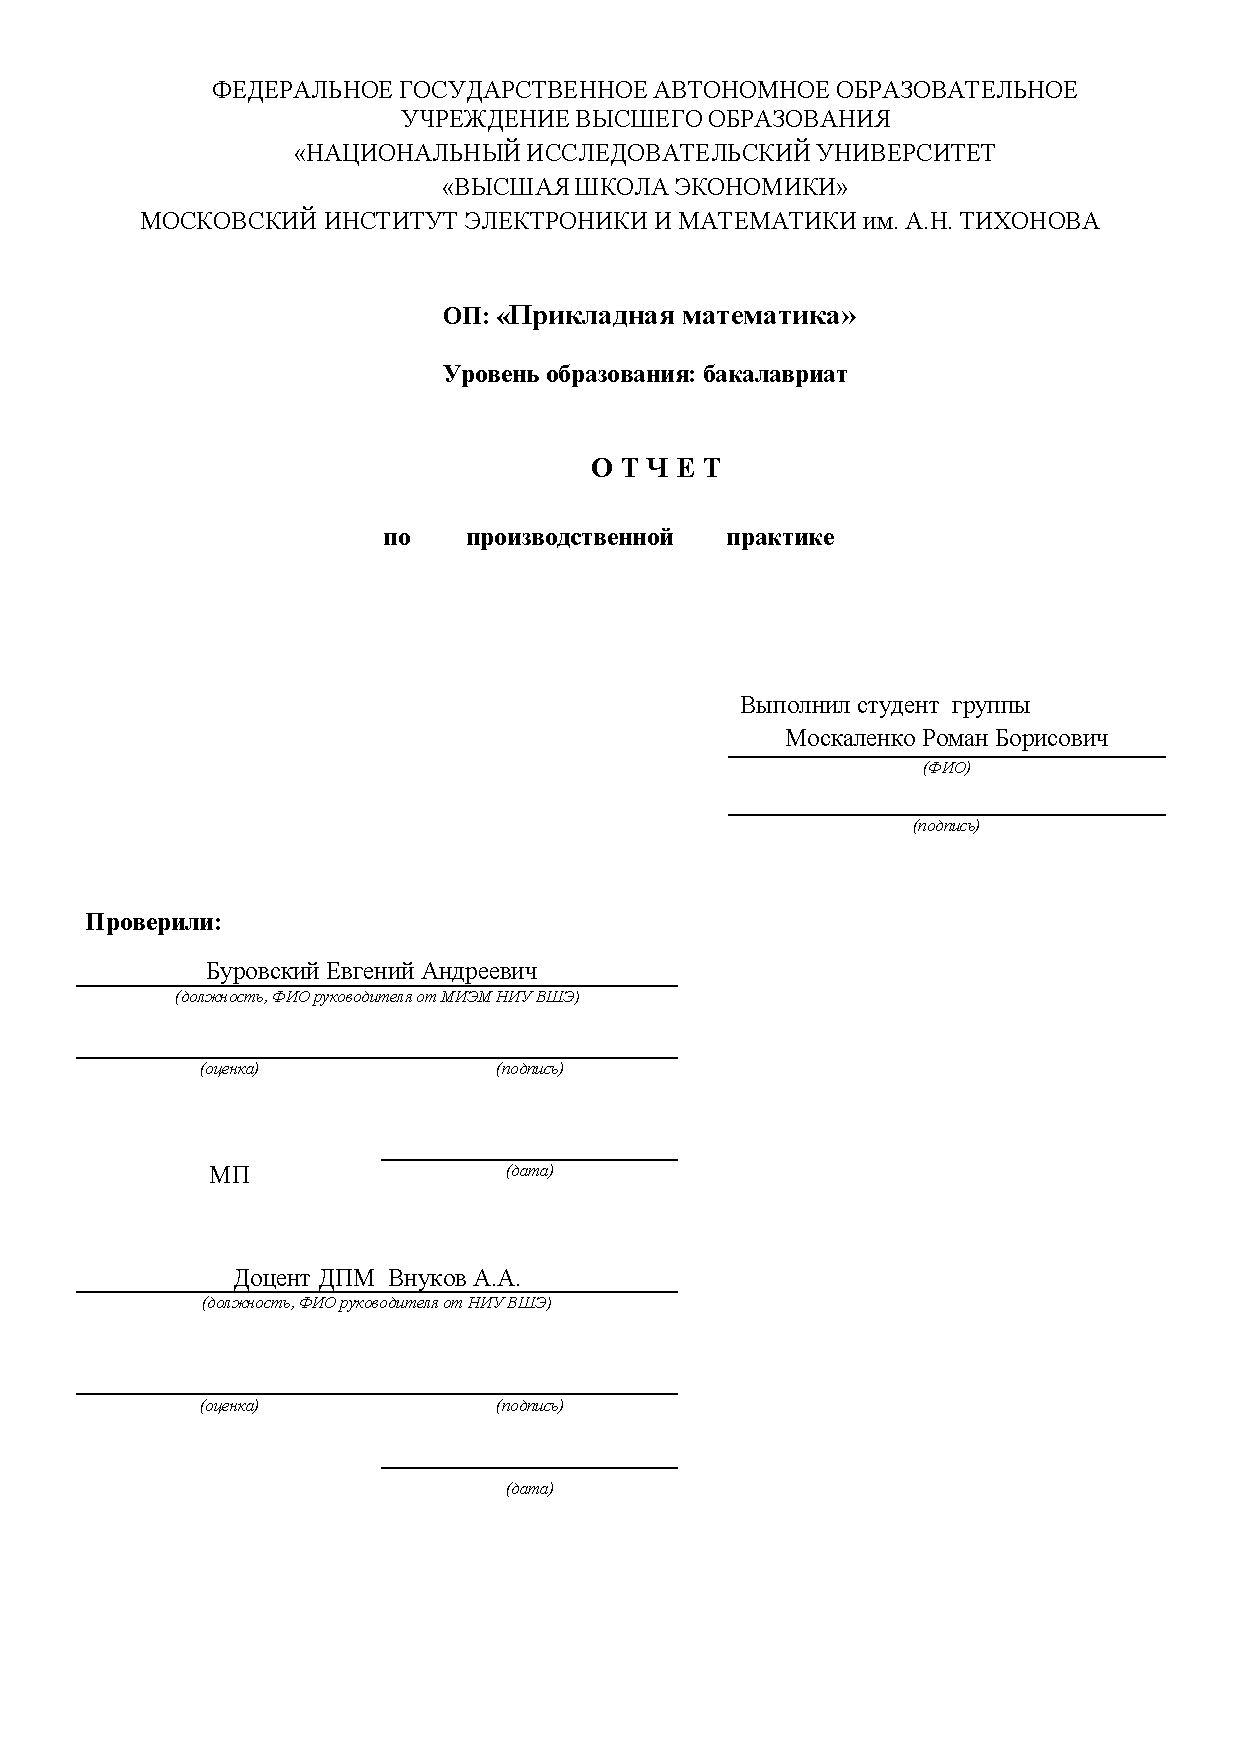
\includepdf[pages=-]{report_header.pdf}


\section{Введение}
%Модель Изинга используется для моделирования и изучения термодинамических свойств. Поведение структуры в модели Изинга сильно зависит от её геометрии. Так например на одно мерных моделях не происходит фазовый переход, но на двумерных моделях переход есть. Но что происходит в промежуточных размерностях? Например если взять какую-то последовательность узлов на двумерной решётке. Именно это и является главным вопросом в данном проекте. 
В данном проекте проводится исследование модели Изинга на фиксированной двумерной конформации. 

Возьмём конформацию(связанную не само пересекающуюся последовательность узлов) на двумерной решётке. Такие конформации можно рассматривать как термодинамическую систему, основанную на модели Изинга, для которых существуют две фазы: плотная(глобулярная) и развёрнутая. Эти фазы соответствуют низким и высоким температурам системы.

\begin{figure}[h]
	\centering
	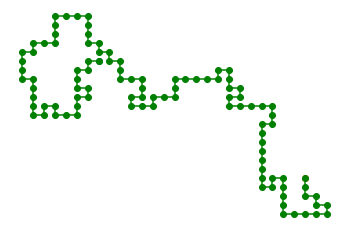
\includegraphics[width=0.45\textwidth]{../images/loose_conf.png}
	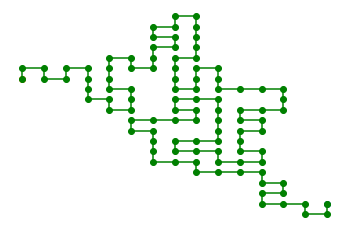
\includegraphics[width=0.45\textwidth]{../images/dense_conf.png} 
	\caption{Пример неплотной и плотной конформации}
\end{figure}

Если посмотреть на изображения конформаций каждого вида, хорошо видно, что плотные конформации по структуре близки с двумерным решёткам, где у каждого узла имеется множество соседей, и развёрнутые конформации наоборот близки к одномерным структурам, где узлы у которых больше 2 соседей встречаются редко. Соответственно можно предположить, что плотные конформации будут иметь свойства схожие с двумерными решётками, а развёрнутые с одномерными.


\subsection{Модель изинга}
Будем рассматривать конформацю как модель Изинга. В каждом узле конформации размещён спин $s_i$ принимающий значения $+1, -1$. Внешнее поле отсутствует. Гамильтониан системы $H = -J\sum_{i, j} s_i s_j$ где $i, j$ индексы соседних узлов, $J$ - коэффициент взаимодействия.

\subsection{Метод Монте-Карло}
Для моделирования системы используется метод Монте-Карло. Мною были реализованы версии с односпиновым и кластернным апдейтом, однако для измерений я использовал кластерную версию. Благодаря отказоустойчивости она работает значительно быстрее, и быстрее сходится, особенно при низких температурах.

На каждой итерации мы выбираем случайный спин и начиная с него начинаем строить кластер из одинаково направленных спинов, добавляя новые спины в кластер с определённой вероятностью. затем мы меняем значения спинов в кластере на противоположные.

\subsection{Цели}
Целью данной работы является исследовать магнитную восприимчивость конформаций, полученных при низких температурах и используя её попробовать определить точку магнитного перехода в конформациях. Так же рассмотреть магнитные свойства конформаций при высоких температурах, и проверить предположение об отсутствии магнитного перехода в них.

\section{Предыдущие результаты}

Ранее при работе на данном проекте был написан программный комплекс для генерации конформаций и расчёта свойств модели Изинга на конформациях. В предыдущих исследованиях мы пытались определить точку магнитного перехода в глобулярных конформациях, для определения точки перехода использовался кумулянт Биндера. Однако оказалось, что только у $60\%$ полученных конформаций намагниченность превышает 0.9 при $\beta = 1$, и большая часть оставшихся конформаций почти не намагничивалась. Из-за большой вариации в значениях намагниченности между конформациями, погрешность при вычислении кумулянта была слишком большой, чтобы точно определить точку перехода. Так же мы пробовали выделить среди полученных конформаций только глобулярные основываясь на их геометрических свойствах, таких как радиус инерции и размеры кластеров вершин (связанных множеств вершин, не имеющих одномерных сегментов внутри себя). Данный подход позволил уменьшить погрешность, но этого оказалось недостаточно для определения точки перехода.

\section{Магнитная восприимчивость} 
Магнитная восприимчивость это отношение намагниченности конформации к напряжённость внешнего поля. Ожидается, что в намагничивающихся конформациях в точке перехода должен наблюдаться пик магнитной восприимчивости, в то время как в не намагничивающихся магнитная восприимчивость не будет иметь пиков.

Получим формулу для магнитной восприимчивости конформации.

По определению
\[
\frac{\partial\langle |M|\rangle}{\partial h}
\]
Подставим формулу намагниченности и продифференцируем.
\[
\frac{\sum_\sigma {|M| e^{-\beta H} \left( -\beta \frac{\partial H}{\partial h}\right)} \cdot Z - \sum_\sigma {|M| e^{-\beta H}} \cdot \sum_\sigma {e^{-\beta H} \left( -\beta \frac{\partial H}{\partial h}\right)}}{Z^2}
\] 

Заметим, что 

\[
\frac{\partial H}{\partial h} = -\sum_i\sigma_i = -|M|
\]
Тогда
\[
\frac{\partial\langle |M|\rangle}{\partial h} = \frac{\sum_\sigma {Z\beta M^2 e^{-\beta H}} - \sum_\sigma {|M| e^{-\beta H}}\cdot \sum_\sigma {\beta |M| e^{-\beta H}}}{Z^2} = \beta \left(\langle M^2\rangle - \langle |M| \rangle^2 \right)
\]


По данной формуле мы можем вычислить магнитную восприимчивость конформаций, используя значения абсолютной намагниченности и квадрата намагниченности, полученные при при расчёте модели Изинга.

\subsection{Результаты замеров}
Для рассмотрения были взяты 10000 конформаций с длинами 250, 500 и 1000. Замеры были сделаны при 10 значениях $\beta$, линейно распределённых от 0.1 до 1.0. 

Все конформации либо имеют единственный пик магнитной восприимчивости, либо магнитная восприимчивость непрерывно возрастает с увеличением $\beta$.

\begin{figure}[htb]
	\centering	
	%% Creator: Matplotlib, PGF backend
%%
%% To include the figure in your LaTeX document, write
%%   \input{<filename>.pgf}
%%
%% Make sure the required packages are loaded in your preamble
%%   \usepackage{pgf}
%%
%% Also ensure that all the required font packages are loaded; for instance,
%% the lmodern package is sometimes necessary when using math font.
%%   \usepackage{lmodern}
%%
%% Figures using additional raster images can only be included by \input if
%% they are in the same directory as the main LaTeX file. For loading figures
%% from other directories you can use the `import` package
%%   \usepackage{import}
%%
%% and then include the figures with
%%   \import{<path to file>}{<filename>.pgf}
%%
%% Matplotlib used the following preamble
%%   
%%   \makeatletter\@ifpackageloaded{underscore}{}{\usepackage[strings]{underscore}}\makeatother
%%
\begingroup%
\makeatletter%
\begin{pgfpicture}%
\pgfpathrectangle{\pgfpointorigin}{\pgfqpoint{4.453681in}{2.871460in}}%
\pgfusepath{use as bounding box, clip}%
\begin{pgfscope}%
\pgfsetbuttcap%
\pgfsetmiterjoin%
\definecolor{currentfill}{rgb}{1.000000,1.000000,1.000000}%
\pgfsetfillcolor{currentfill}%
\pgfsetlinewidth{0.000000pt}%
\definecolor{currentstroke}{rgb}{1.000000,1.000000,1.000000}%
\pgfsetstrokecolor{currentstroke}%
\pgfsetdash{}{0pt}%
\pgfpathmoveto{\pgfqpoint{0.000000in}{0.000000in}}%
\pgfpathlineto{\pgfqpoint{4.453681in}{0.000000in}}%
\pgfpathlineto{\pgfqpoint{4.453681in}{2.871460in}}%
\pgfpathlineto{\pgfqpoint{0.000000in}{2.871460in}}%
\pgfpathlineto{\pgfqpoint{0.000000in}{0.000000in}}%
\pgfpathclose%
\pgfusepath{fill}%
\end{pgfscope}%
\begin{pgfscope}%
\pgfsetbuttcap%
\pgfsetmiterjoin%
\definecolor{currentfill}{rgb}{1.000000,1.000000,1.000000}%
\pgfsetfillcolor{currentfill}%
\pgfsetlinewidth{0.000000pt}%
\definecolor{currentstroke}{rgb}{0.000000,0.000000,0.000000}%
\pgfsetstrokecolor{currentstroke}%
\pgfsetstrokeopacity{0.000000}%
\pgfsetdash{}{0pt}%
\pgfpathmoveto{\pgfqpoint{0.654013in}{0.499691in}}%
\pgfpathlineto{\pgfqpoint{4.353681in}{0.499691in}}%
\pgfpathlineto{\pgfqpoint{4.353681in}{2.771460in}}%
\pgfpathlineto{\pgfqpoint{0.654013in}{2.771460in}}%
\pgfpathlineto{\pgfqpoint{0.654013in}{0.499691in}}%
\pgfpathclose%
\pgfusepath{fill}%
\end{pgfscope}%
\begin{pgfscope}%
\pgfpathrectangle{\pgfqpoint{0.654013in}{0.499691in}}{\pgfqpoint{3.699668in}{2.271769in}}%
\pgfusepath{clip}%
\pgfsetbuttcap%
\pgfsetmiterjoin%
\definecolor{currentfill}{rgb}{0.121569,0.466667,0.705882}%
\pgfsetfillcolor{currentfill}%
\pgfsetlinewidth{0.000000pt}%
\definecolor{currentstroke}{rgb}{0.000000,0.000000,0.000000}%
\pgfsetstrokecolor{currentstroke}%
\pgfsetstrokeopacity{0.000000}%
\pgfsetdash{}{0pt}%
\pgfpathmoveto{\pgfqpoint{0.822180in}{0.499691in}}%
\pgfpathlineto{\pgfqpoint{0.859970in}{0.499691in}}%
\pgfpathlineto{\pgfqpoint{0.859970in}{1.830176in}}%
\pgfpathlineto{\pgfqpoint{0.822180in}{1.830176in}}%
\pgfpathlineto{\pgfqpoint{0.822180in}{0.499691in}}%
\pgfpathclose%
\pgfusepath{fill}%
\end{pgfscope}%
\begin{pgfscope}%
\pgfpathrectangle{\pgfqpoint{0.654013in}{0.499691in}}{\pgfqpoint{3.699668in}{2.271769in}}%
\pgfusepath{clip}%
\pgfsetbuttcap%
\pgfsetmiterjoin%
\definecolor{currentfill}{rgb}{0.121569,0.466667,0.705882}%
\pgfsetfillcolor{currentfill}%
\pgfsetlinewidth{0.000000pt}%
\definecolor{currentstroke}{rgb}{0.000000,0.000000,0.000000}%
\pgfsetstrokecolor{currentstroke}%
\pgfsetstrokeopacity{0.000000}%
\pgfsetdash{}{0pt}%
\pgfpathmoveto{\pgfqpoint{1.011131in}{0.499691in}}%
\pgfpathlineto{\pgfqpoint{1.048921in}{0.499691in}}%
\pgfpathlineto{\pgfqpoint{1.048921in}{0.499691in}}%
\pgfpathlineto{\pgfqpoint{1.011131in}{0.499691in}}%
\pgfpathlineto{\pgfqpoint{1.011131in}{0.499691in}}%
\pgfpathclose%
\pgfusepath{fill}%
\end{pgfscope}%
\begin{pgfscope}%
\pgfpathrectangle{\pgfqpoint{0.654013in}{0.499691in}}{\pgfqpoint{3.699668in}{2.271769in}}%
\pgfusepath{clip}%
\pgfsetbuttcap%
\pgfsetmiterjoin%
\definecolor{currentfill}{rgb}{0.121569,0.466667,0.705882}%
\pgfsetfillcolor{currentfill}%
\pgfsetlinewidth{0.000000pt}%
\definecolor{currentstroke}{rgb}{0.000000,0.000000,0.000000}%
\pgfsetstrokecolor{currentstroke}%
\pgfsetstrokeopacity{0.000000}%
\pgfsetdash{}{0pt}%
\pgfpathmoveto{\pgfqpoint{1.200083in}{0.499691in}}%
\pgfpathlineto{\pgfqpoint{1.237873in}{0.499691in}}%
\pgfpathlineto{\pgfqpoint{1.237873in}{0.499691in}}%
\pgfpathlineto{\pgfqpoint{1.200083in}{0.499691in}}%
\pgfpathlineto{\pgfqpoint{1.200083in}{0.499691in}}%
\pgfpathclose%
\pgfusepath{fill}%
\end{pgfscope}%
\begin{pgfscope}%
\pgfpathrectangle{\pgfqpoint{0.654013in}{0.499691in}}{\pgfqpoint{3.699668in}{2.271769in}}%
\pgfusepath{clip}%
\pgfsetbuttcap%
\pgfsetmiterjoin%
\definecolor{currentfill}{rgb}{0.121569,0.466667,0.705882}%
\pgfsetfillcolor{currentfill}%
\pgfsetlinewidth{0.000000pt}%
\definecolor{currentstroke}{rgb}{0.000000,0.000000,0.000000}%
\pgfsetstrokecolor{currentstroke}%
\pgfsetstrokeopacity{0.000000}%
\pgfsetdash{}{0pt}%
\pgfpathmoveto{\pgfqpoint{1.389034in}{0.499691in}}%
\pgfpathlineto{\pgfqpoint{1.426824in}{0.499691in}}%
\pgfpathlineto{\pgfqpoint{1.426824in}{1.538228in}}%
\pgfpathlineto{\pgfqpoint{1.389034in}{1.538228in}}%
\pgfpathlineto{\pgfqpoint{1.389034in}{0.499691in}}%
\pgfpathclose%
\pgfusepath{fill}%
\end{pgfscope}%
\begin{pgfscope}%
\pgfpathrectangle{\pgfqpoint{0.654013in}{0.499691in}}{\pgfqpoint{3.699668in}{2.271769in}}%
\pgfusepath{clip}%
\pgfsetbuttcap%
\pgfsetmiterjoin%
\definecolor{currentfill}{rgb}{0.121569,0.466667,0.705882}%
\pgfsetfillcolor{currentfill}%
\pgfsetlinewidth{0.000000pt}%
\definecolor{currentstroke}{rgb}{0.000000,0.000000,0.000000}%
\pgfsetstrokecolor{currentstroke}%
\pgfsetstrokeopacity{0.000000}%
\pgfsetdash{}{0pt}%
\pgfpathmoveto{\pgfqpoint{1.577985in}{0.499691in}}%
\pgfpathlineto{\pgfqpoint{1.615776in}{0.499691in}}%
\pgfpathlineto{\pgfqpoint{1.615776in}{0.499691in}}%
\pgfpathlineto{\pgfqpoint{1.577985in}{0.499691in}}%
\pgfpathlineto{\pgfqpoint{1.577985in}{0.499691in}}%
\pgfpathclose%
\pgfusepath{fill}%
\end{pgfscope}%
\begin{pgfscope}%
\pgfpathrectangle{\pgfqpoint{0.654013in}{0.499691in}}{\pgfqpoint{3.699668in}{2.271769in}}%
\pgfusepath{clip}%
\pgfsetbuttcap%
\pgfsetmiterjoin%
\definecolor{currentfill}{rgb}{0.121569,0.466667,0.705882}%
\pgfsetfillcolor{currentfill}%
\pgfsetlinewidth{0.000000pt}%
\definecolor{currentstroke}{rgb}{0.000000,0.000000,0.000000}%
\pgfsetstrokecolor{currentstroke}%
\pgfsetstrokeopacity{0.000000}%
\pgfsetdash{}{0pt}%
\pgfpathmoveto{\pgfqpoint{1.766937in}{0.499691in}}%
\pgfpathlineto{\pgfqpoint{1.804727in}{0.499691in}}%
\pgfpathlineto{\pgfqpoint{1.804727in}{0.499691in}}%
\pgfpathlineto{\pgfqpoint{1.766937in}{0.499691in}}%
\pgfpathlineto{\pgfqpoint{1.766937in}{0.499691in}}%
\pgfpathclose%
\pgfusepath{fill}%
\end{pgfscope}%
\begin{pgfscope}%
\pgfpathrectangle{\pgfqpoint{0.654013in}{0.499691in}}{\pgfqpoint{3.699668in}{2.271769in}}%
\pgfusepath{clip}%
\pgfsetbuttcap%
\pgfsetmiterjoin%
\definecolor{currentfill}{rgb}{0.121569,0.466667,0.705882}%
\pgfsetfillcolor{currentfill}%
\pgfsetlinewidth{0.000000pt}%
\definecolor{currentstroke}{rgb}{0.000000,0.000000,0.000000}%
\pgfsetstrokecolor{currentstroke}%
\pgfsetstrokeopacity{0.000000}%
\pgfsetdash{}{0pt}%
\pgfpathmoveto{\pgfqpoint{1.955888in}{0.499691in}}%
\pgfpathlineto{\pgfqpoint{1.993678in}{0.499691in}}%
\pgfpathlineto{\pgfqpoint{1.993678in}{0.499691in}}%
\pgfpathlineto{\pgfqpoint{1.955888in}{0.499691in}}%
\pgfpathlineto{\pgfqpoint{1.955888in}{0.499691in}}%
\pgfpathclose%
\pgfusepath{fill}%
\end{pgfscope}%
\begin{pgfscope}%
\pgfpathrectangle{\pgfqpoint{0.654013in}{0.499691in}}{\pgfqpoint{3.699668in}{2.271769in}}%
\pgfusepath{clip}%
\pgfsetbuttcap%
\pgfsetmiterjoin%
\definecolor{currentfill}{rgb}{0.121569,0.466667,0.705882}%
\pgfsetfillcolor{currentfill}%
\pgfsetlinewidth{0.000000pt}%
\definecolor{currentstroke}{rgb}{0.000000,0.000000,0.000000}%
\pgfsetstrokecolor{currentstroke}%
\pgfsetstrokeopacity{0.000000}%
\pgfsetdash{}{0pt}%
\pgfpathmoveto{\pgfqpoint{2.144839in}{0.499691in}}%
\pgfpathlineto{\pgfqpoint{2.182630in}{0.499691in}}%
\pgfpathlineto{\pgfqpoint{2.182630in}{0.662038in}}%
\pgfpathlineto{\pgfqpoint{2.144839in}{0.662038in}}%
\pgfpathlineto{\pgfqpoint{2.144839in}{0.499691in}}%
\pgfpathclose%
\pgfusepath{fill}%
\end{pgfscope}%
\begin{pgfscope}%
\pgfpathrectangle{\pgfqpoint{0.654013in}{0.499691in}}{\pgfqpoint{3.699668in}{2.271769in}}%
\pgfusepath{clip}%
\pgfsetbuttcap%
\pgfsetmiterjoin%
\definecolor{currentfill}{rgb}{0.121569,0.466667,0.705882}%
\pgfsetfillcolor{currentfill}%
\pgfsetlinewidth{0.000000pt}%
\definecolor{currentstroke}{rgb}{0.000000,0.000000,0.000000}%
\pgfsetstrokecolor{currentstroke}%
\pgfsetstrokeopacity{0.000000}%
\pgfsetdash{}{0pt}%
\pgfpathmoveto{\pgfqpoint{2.333791in}{0.499691in}}%
\pgfpathlineto{\pgfqpoint{2.371581in}{0.499691in}}%
\pgfpathlineto{\pgfqpoint{2.371581in}{0.499691in}}%
\pgfpathlineto{\pgfqpoint{2.333791in}{0.499691in}}%
\pgfpathlineto{\pgfqpoint{2.333791in}{0.499691in}}%
\pgfpathclose%
\pgfusepath{fill}%
\end{pgfscope}%
\begin{pgfscope}%
\pgfpathrectangle{\pgfqpoint{0.654013in}{0.499691in}}{\pgfqpoint{3.699668in}{2.271769in}}%
\pgfusepath{clip}%
\pgfsetbuttcap%
\pgfsetmiterjoin%
\definecolor{currentfill}{rgb}{0.121569,0.466667,0.705882}%
\pgfsetfillcolor{currentfill}%
\pgfsetlinewidth{0.000000pt}%
\definecolor{currentstroke}{rgb}{0.000000,0.000000,0.000000}%
\pgfsetstrokecolor{currentstroke}%
\pgfsetstrokeopacity{0.000000}%
\pgfsetdash{}{0pt}%
\pgfpathmoveto{\pgfqpoint{2.522742in}{0.499691in}}%
\pgfpathlineto{\pgfqpoint{2.560532in}{0.499691in}}%
\pgfpathlineto{\pgfqpoint{2.560532in}{0.499691in}}%
\pgfpathlineto{\pgfqpoint{2.522742in}{0.499691in}}%
\pgfpathlineto{\pgfqpoint{2.522742in}{0.499691in}}%
\pgfpathclose%
\pgfusepath{fill}%
\end{pgfscope}%
\begin{pgfscope}%
\pgfpathrectangle{\pgfqpoint{0.654013in}{0.499691in}}{\pgfqpoint{3.699668in}{2.271769in}}%
\pgfusepath{clip}%
\pgfsetbuttcap%
\pgfsetmiterjoin%
\definecolor{currentfill}{rgb}{0.121569,0.466667,0.705882}%
\pgfsetfillcolor{currentfill}%
\pgfsetlinewidth{0.000000pt}%
\definecolor{currentstroke}{rgb}{0.000000,0.000000,0.000000}%
\pgfsetstrokecolor{currentstroke}%
\pgfsetstrokeopacity{0.000000}%
\pgfsetdash{}{0pt}%
\pgfpathmoveto{\pgfqpoint{2.711694in}{0.499691in}}%
\pgfpathlineto{\pgfqpoint{2.749484in}{0.499691in}}%
\pgfpathlineto{\pgfqpoint{2.749484in}{0.560700in}}%
\pgfpathlineto{\pgfqpoint{2.711694in}{0.560700in}}%
\pgfpathlineto{\pgfqpoint{2.711694in}{0.499691in}}%
\pgfpathclose%
\pgfusepath{fill}%
\end{pgfscope}%
\begin{pgfscope}%
\pgfpathrectangle{\pgfqpoint{0.654013in}{0.499691in}}{\pgfqpoint{3.699668in}{2.271769in}}%
\pgfusepath{clip}%
\pgfsetbuttcap%
\pgfsetmiterjoin%
\definecolor{currentfill}{rgb}{0.121569,0.466667,0.705882}%
\pgfsetfillcolor{currentfill}%
\pgfsetlinewidth{0.000000pt}%
\definecolor{currentstroke}{rgb}{0.000000,0.000000,0.000000}%
\pgfsetstrokecolor{currentstroke}%
\pgfsetstrokeopacity{0.000000}%
\pgfsetdash{}{0pt}%
\pgfpathmoveto{\pgfqpoint{2.900645in}{0.499691in}}%
\pgfpathlineto{\pgfqpoint{2.938435in}{0.499691in}}%
\pgfpathlineto{\pgfqpoint{2.938435in}{0.499691in}}%
\pgfpathlineto{\pgfqpoint{2.900645in}{0.499691in}}%
\pgfpathlineto{\pgfqpoint{2.900645in}{0.499691in}}%
\pgfpathclose%
\pgfusepath{fill}%
\end{pgfscope}%
\begin{pgfscope}%
\pgfpathrectangle{\pgfqpoint{0.654013in}{0.499691in}}{\pgfqpoint{3.699668in}{2.271769in}}%
\pgfusepath{clip}%
\pgfsetbuttcap%
\pgfsetmiterjoin%
\definecolor{currentfill}{rgb}{0.121569,0.466667,0.705882}%
\pgfsetfillcolor{currentfill}%
\pgfsetlinewidth{0.000000pt}%
\definecolor{currentstroke}{rgb}{0.000000,0.000000,0.000000}%
\pgfsetstrokecolor{currentstroke}%
\pgfsetstrokeopacity{0.000000}%
\pgfsetdash{}{0pt}%
\pgfpathmoveto{\pgfqpoint{3.089596in}{0.499691in}}%
\pgfpathlineto{\pgfqpoint{3.127387in}{0.499691in}}%
\pgfpathlineto{\pgfqpoint{3.127387in}{0.499691in}}%
\pgfpathlineto{\pgfqpoint{3.089596in}{0.499691in}}%
\pgfpathlineto{\pgfqpoint{3.089596in}{0.499691in}}%
\pgfpathclose%
\pgfusepath{fill}%
\end{pgfscope}%
\begin{pgfscope}%
\pgfpathrectangle{\pgfqpoint{0.654013in}{0.499691in}}{\pgfqpoint{3.699668in}{2.271769in}}%
\pgfusepath{clip}%
\pgfsetbuttcap%
\pgfsetmiterjoin%
\definecolor{currentfill}{rgb}{0.121569,0.466667,0.705882}%
\pgfsetfillcolor{currentfill}%
\pgfsetlinewidth{0.000000pt}%
\definecolor{currentstroke}{rgb}{0.000000,0.000000,0.000000}%
\pgfsetstrokecolor{currentstroke}%
\pgfsetstrokeopacity{0.000000}%
\pgfsetdash{}{0pt}%
\pgfpathmoveto{\pgfqpoint{3.278548in}{0.499691in}}%
\pgfpathlineto{\pgfqpoint{3.316338in}{0.499691in}}%
\pgfpathlineto{\pgfqpoint{3.316338in}{0.499691in}}%
\pgfpathlineto{\pgfqpoint{3.278548in}{0.499691in}}%
\pgfpathlineto{\pgfqpoint{3.278548in}{0.499691in}}%
\pgfpathclose%
\pgfusepath{fill}%
\end{pgfscope}%
\begin{pgfscope}%
\pgfpathrectangle{\pgfqpoint{0.654013in}{0.499691in}}{\pgfqpoint{3.699668in}{2.271769in}}%
\pgfusepath{clip}%
\pgfsetbuttcap%
\pgfsetmiterjoin%
\definecolor{currentfill}{rgb}{0.121569,0.466667,0.705882}%
\pgfsetfillcolor{currentfill}%
\pgfsetlinewidth{0.000000pt}%
\definecolor{currentstroke}{rgb}{0.000000,0.000000,0.000000}%
\pgfsetstrokecolor{currentstroke}%
\pgfsetstrokeopacity{0.000000}%
\pgfsetdash{}{0pt}%
\pgfpathmoveto{\pgfqpoint{3.467499in}{0.499691in}}%
\pgfpathlineto{\pgfqpoint{3.505289in}{0.499691in}}%
\pgfpathlineto{\pgfqpoint{3.505289in}{0.546568in}}%
\pgfpathlineto{\pgfqpoint{3.467499in}{0.546568in}}%
\pgfpathlineto{\pgfqpoint{3.467499in}{0.499691in}}%
\pgfpathclose%
\pgfusepath{fill}%
\end{pgfscope}%
\begin{pgfscope}%
\pgfpathrectangle{\pgfqpoint{0.654013in}{0.499691in}}{\pgfqpoint{3.699668in}{2.271769in}}%
\pgfusepath{clip}%
\pgfsetbuttcap%
\pgfsetmiterjoin%
\definecolor{currentfill}{rgb}{0.121569,0.466667,0.705882}%
\pgfsetfillcolor{currentfill}%
\pgfsetlinewidth{0.000000pt}%
\definecolor{currentstroke}{rgb}{0.000000,0.000000,0.000000}%
\pgfsetstrokecolor{currentstroke}%
\pgfsetstrokeopacity{0.000000}%
\pgfsetdash{}{0pt}%
\pgfpathmoveto{\pgfqpoint{3.656450in}{0.499691in}}%
\pgfpathlineto{\pgfqpoint{3.694241in}{0.499691in}}%
\pgfpathlineto{\pgfqpoint{3.694241in}{0.499691in}}%
\pgfpathlineto{\pgfqpoint{3.656450in}{0.499691in}}%
\pgfpathlineto{\pgfqpoint{3.656450in}{0.499691in}}%
\pgfpathclose%
\pgfusepath{fill}%
\end{pgfscope}%
\begin{pgfscope}%
\pgfpathrectangle{\pgfqpoint{0.654013in}{0.499691in}}{\pgfqpoint{3.699668in}{2.271769in}}%
\pgfusepath{clip}%
\pgfsetbuttcap%
\pgfsetmiterjoin%
\definecolor{currentfill}{rgb}{0.121569,0.466667,0.705882}%
\pgfsetfillcolor{currentfill}%
\pgfsetlinewidth{0.000000pt}%
\definecolor{currentstroke}{rgb}{0.000000,0.000000,0.000000}%
\pgfsetstrokecolor{currentstroke}%
\pgfsetstrokeopacity{0.000000}%
\pgfsetdash{}{0pt}%
\pgfpathmoveto{\pgfqpoint{3.845402in}{0.499691in}}%
\pgfpathlineto{\pgfqpoint{3.883192in}{0.499691in}}%
\pgfpathlineto{\pgfqpoint{3.883192in}{0.499691in}}%
\pgfpathlineto{\pgfqpoint{3.845402in}{0.499691in}}%
\pgfpathlineto{\pgfqpoint{3.845402in}{0.499691in}}%
\pgfpathclose%
\pgfusepath{fill}%
\end{pgfscope}%
\begin{pgfscope}%
\pgfpathrectangle{\pgfqpoint{0.654013in}{0.499691in}}{\pgfqpoint{3.699668in}{2.271769in}}%
\pgfusepath{clip}%
\pgfsetbuttcap%
\pgfsetmiterjoin%
\definecolor{currentfill}{rgb}{0.121569,0.466667,0.705882}%
\pgfsetfillcolor{currentfill}%
\pgfsetlinewidth{0.000000pt}%
\definecolor{currentstroke}{rgb}{0.000000,0.000000,0.000000}%
\pgfsetstrokecolor{currentstroke}%
\pgfsetstrokeopacity{0.000000}%
\pgfsetdash{}{0pt}%
\pgfpathmoveto{\pgfqpoint{4.034353in}{0.499691in}}%
\pgfpathlineto{\pgfqpoint{4.072143in}{0.499691in}}%
\pgfpathlineto{\pgfqpoint{4.072143in}{1.307289in}}%
\pgfpathlineto{\pgfqpoint{4.034353in}{1.307289in}}%
\pgfpathlineto{\pgfqpoint{4.034353in}{0.499691in}}%
\pgfpathclose%
\pgfusepath{fill}%
\end{pgfscope}%
\begin{pgfscope}%
\pgfpathrectangle{\pgfqpoint{0.654013in}{0.499691in}}{\pgfqpoint{3.699668in}{2.271769in}}%
\pgfusepath{clip}%
\pgfsetbuttcap%
\pgfsetmiterjoin%
\definecolor{currentfill}{rgb}{1.000000,0.498039,0.054902}%
\pgfsetfillcolor{currentfill}%
\pgfsetlinewidth{0.000000pt}%
\definecolor{currentstroke}{rgb}{0.000000,0.000000,0.000000}%
\pgfsetstrokecolor{currentstroke}%
\pgfsetstrokeopacity{0.000000}%
\pgfsetdash{}{0pt}%
\pgfpathmoveto{\pgfqpoint{0.859970in}{0.499691in}}%
\pgfpathlineto{\pgfqpoint{0.897760in}{0.499691in}}%
\pgfpathlineto{\pgfqpoint{0.897760in}{2.358234in}}%
\pgfpathlineto{\pgfqpoint{0.859970in}{2.358234in}}%
\pgfpathlineto{\pgfqpoint{0.859970in}{0.499691in}}%
\pgfpathclose%
\pgfusepath{fill}%
\end{pgfscope}%
\begin{pgfscope}%
\pgfpathrectangle{\pgfqpoint{0.654013in}{0.499691in}}{\pgfqpoint{3.699668in}{2.271769in}}%
\pgfusepath{clip}%
\pgfsetbuttcap%
\pgfsetmiterjoin%
\definecolor{currentfill}{rgb}{1.000000,0.498039,0.054902}%
\pgfsetfillcolor{currentfill}%
\pgfsetlinewidth{0.000000pt}%
\definecolor{currentstroke}{rgb}{0.000000,0.000000,0.000000}%
\pgfsetstrokecolor{currentstroke}%
\pgfsetstrokeopacity{0.000000}%
\pgfsetdash{}{0pt}%
\pgfpathmoveto{\pgfqpoint{1.048921in}{0.499691in}}%
\pgfpathlineto{\pgfqpoint{1.086712in}{0.499691in}}%
\pgfpathlineto{\pgfqpoint{1.086712in}{0.499691in}}%
\pgfpathlineto{\pgfqpoint{1.048921in}{0.499691in}}%
\pgfpathlineto{\pgfqpoint{1.048921in}{0.499691in}}%
\pgfpathclose%
\pgfusepath{fill}%
\end{pgfscope}%
\begin{pgfscope}%
\pgfpathrectangle{\pgfqpoint{0.654013in}{0.499691in}}{\pgfqpoint{3.699668in}{2.271769in}}%
\pgfusepath{clip}%
\pgfsetbuttcap%
\pgfsetmiterjoin%
\definecolor{currentfill}{rgb}{1.000000,0.498039,0.054902}%
\pgfsetfillcolor{currentfill}%
\pgfsetlinewidth{0.000000pt}%
\definecolor{currentstroke}{rgb}{0.000000,0.000000,0.000000}%
\pgfsetstrokecolor{currentstroke}%
\pgfsetstrokeopacity{0.000000}%
\pgfsetdash{}{0pt}%
\pgfpathmoveto{\pgfqpoint{1.237873in}{0.499691in}}%
\pgfpathlineto{\pgfqpoint{1.275663in}{0.499691in}}%
\pgfpathlineto{\pgfqpoint{1.275663in}{0.499691in}}%
\pgfpathlineto{\pgfqpoint{1.237873in}{0.499691in}}%
\pgfpathlineto{\pgfqpoint{1.237873in}{0.499691in}}%
\pgfpathclose%
\pgfusepath{fill}%
\end{pgfscope}%
\begin{pgfscope}%
\pgfpathrectangle{\pgfqpoint{0.654013in}{0.499691in}}{\pgfqpoint{3.699668in}{2.271769in}}%
\pgfusepath{clip}%
\pgfsetbuttcap%
\pgfsetmiterjoin%
\definecolor{currentfill}{rgb}{1.000000,0.498039,0.054902}%
\pgfsetfillcolor{currentfill}%
\pgfsetlinewidth{0.000000pt}%
\definecolor{currentstroke}{rgb}{0.000000,0.000000,0.000000}%
\pgfsetstrokecolor{currentstroke}%
\pgfsetstrokeopacity{0.000000}%
\pgfsetdash{}{0pt}%
\pgfpathmoveto{\pgfqpoint{1.426824in}{0.499691in}}%
\pgfpathlineto{\pgfqpoint{1.464614in}{0.499691in}}%
\pgfpathlineto{\pgfqpoint{1.464614in}{1.066698in}}%
\pgfpathlineto{\pgfqpoint{1.426824in}{1.066698in}}%
\pgfpathlineto{\pgfqpoint{1.426824in}{0.499691in}}%
\pgfpathclose%
\pgfusepath{fill}%
\end{pgfscope}%
\begin{pgfscope}%
\pgfpathrectangle{\pgfqpoint{0.654013in}{0.499691in}}{\pgfqpoint{3.699668in}{2.271769in}}%
\pgfusepath{clip}%
\pgfsetbuttcap%
\pgfsetmiterjoin%
\definecolor{currentfill}{rgb}{1.000000,0.498039,0.054902}%
\pgfsetfillcolor{currentfill}%
\pgfsetlinewidth{0.000000pt}%
\definecolor{currentstroke}{rgb}{0.000000,0.000000,0.000000}%
\pgfsetstrokecolor{currentstroke}%
\pgfsetstrokeopacity{0.000000}%
\pgfsetdash{}{0pt}%
\pgfpathmoveto{\pgfqpoint{1.615776in}{0.499691in}}%
\pgfpathlineto{\pgfqpoint{1.653566in}{0.499691in}}%
\pgfpathlineto{\pgfqpoint{1.653566in}{0.499691in}}%
\pgfpathlineto{\pgfqpoint{1.615776in}{0.499691in}}%
\pgfpathlineto{\pgfqpoint{1.615776in}{0.499691in}}%
\pgfpathclose%
\pgfusepath{fill}%
\end{pgfscope}%
\begin{pgfscope}%
\pgfpathrectangle{\pgfqpoint{0.654013in}{0.499691in}}{\pgfqpoint{3.699668in}{2.271769in}}%
\pgfusepath{clip}%
\pgfsetbuttcap%
\pgfsetmiterjoin%
\definecolor{currentfill}{rgb}{1.000000,0.498039,0.054902}%
\pgfsetfillcolor{currentfill}%
\pgfsetlinewidth{0.000000pt}%
\definecolor{currentstroke}{rgb}{0.000000,0.000000,0.000000}%
\pgfsetstrokecolor{currentstroke}%
\pgfsetstrokeopacity{0.000000}%
\pgfsetdash{}{0pt}%
\pgfpathmoveto{\pgfqpoint{1.804727in}{0.499691in}}%
\pgfpathlineto{\pgfqpoint{1.842517in}{0.499691in}}%
\pgfpathlineto{\pgfqpoint{1.842517in}{0.499691in}}%
\pgfpathlineto{\pgfqpoint{1.804727in}{0.499691in}}%
\pgfpathlineto{\pgfqpoint{1.804727in}{0.499691in}}%
\pgfpathclose%
\pgfusepath{fill}%
\end{pgfscope}%
\begin{pgfscope}%
\pgfpathrectangle{\pgfqpoint{0.654013in}{0.499691in}}{\pgfqpoint{3.699668in}{2.271769in}}%
\pgfusepath{clip}%
\pgfsetbuttcap%
\pgfsetmiterjoin%
\definecolor{currentfill}{rgb}{1.000000,0.498039,0.054902}%
\pgfsetfillcolor{currentfill}%
\pgfsetlinewidth{0.000000pt}%
\definecolor{currentstroke}{rgb}{0.000000,0.000000,0.000000}%
\pgfsetstrokecolor{currentstroke}%
\pgfsetstrokeopacity{0.000000}%
\pgfsetdash{}{0pt}%
\pgfpathmoveto{\pgfqpoint{1.993678in}{0.499691in}}%
\pgfpathlineto{\pgfqpoint{2.031469in}{0.499691in}}%
\pgfpathlineto{\pgfqpoint{2.031469in}{0.499691in}}%
\pgfpathlineto{\pgfqpoint{1.993678in}{0.499691in}}%
\pgfpathlineto{\pgfqpoint{1.993678in}{0.499691in}}%
\pgfpathclose%
\pgfusepath{fill}%
\end{pgfscope}%
\begin{pgfscope}%
\pgfpathrectangle{\pgfqpoint{0.654013in}{0.499691in}}{\pgfqpoint{3.699668in}{2.271769in}}%
\pgfusepath{clip}%
\pgfsetbuttcap%
\pgfsetmiterjoin%
\definecolor{currentfill}{rgb}{1.000000,0.498039,0.054902}%
\pgfsetfillcolor{currentfill}%
\pgfsetlinewidth{0.000000pt}%
\definecolor{currentstroke}{rgb}{0.000000,0.000000,0.000000}%
\pgfsetstrokecolor{currentstroke}%
\pgfsetstrokeopacity{0.000000}%
\pgfsetdash{}{0pt}%
\pgfpathmoveto{\pgfqpoint{2.182630in}{0.499691in}}%
\pgfpathlineto{\pgfqpoint{2.220420in}{0.499691in}}%
\pgfpathlineto{\pgfqpoint{2.220420in}{0.567939in}}%
\pgfpathlineto{\pgfqpoint{2.182630in}{0.567939in}}%
\pgfpathlineto{\pgfqpoint{2.182630in}{0.499691in}}%
\pgfpathclose%
\pgfusepath{fill}%
\end{pgfscope}%
\begin{pgfscope}%
\pgfpathrectangle{\pgfqpoint{0.654013in}{0.499691in}}{\pgfqpoint{3.699668in}{2.271769in}}%
\pgfusepath{clip}%
\pgfsetbuttcap%
\pgfsetmiterjoin%
\definecolor{currentfill}{rgb}{1.000000,0.498039,0.054902}%
\pgfsetfillcolor{currentfill}%
\pgfsetlinewidth{0.000000pt}%
\definecolor{currentstroke}{rgb}{0.000000,0.000000,0.000000}%
\pgfsetstrokecolor{currentstroke}%
\pgfsetstrokeopacity{0.000000}%
\pgfsetdash{}{0pt}%
\pgfpathmoveto{\pgfqpoint{2.371581in}{0.499691in}}%
\pgfpathlineto{\pgfqpoint{2.409371in}{0.499691in}}%
\pgfpathlineto{\pgfqpoint{2.409371in}{0.499691in}}%
\pgfpathlineto{\pgfqpoint{2.371581in}{0.499691in}}%
\pgfpathlineto{\pgfqpoint{2.371581in}{0.499691in}}%
\pgfpathclose%
\pgfusepath{fill}%
\end{pgfscope}%
\begin{pgfscope}%
\pgfpathrectangle{\pgfqpoint{0.654013in}{0.499691in}}{\pgfqpoint{3.699668in}{2.271769in}}%
\pgfusepath{clip}%
\pgfsetbuttcap%
\pgfsetmiterjoin%
\definecolor{currentfill}{rgb}{1.000000,0.498039,0.054902}%
\pgfsetfillcolor{currentfill}%
\pgfsetlinewidth{0.000000pt}%
\definecolor{currentstroke}{rgb}{0.000000,0.000000,0.000000}%
\pgfsetstrokecolor{currentstroke}%
\pgfsetstrokeopacity{0.000000}%
\pgfsetdash{}{0pt}%
\pgfpathmoveto{\pgfqpoint{2.560532in}{0.499691in}}%
\pgfpathlineto{\pgfqpoint{2.598323in}{0.499691in}}%
\pgfpathlineto{\pgfqpoint{2.598323in}{0.499691in}}%
\pgfpathlineto{\pgfqpoint{2.560532in}{0.499691in}}%
\pgfpathlineto{\pgfqpoint{2.560532in}{0.499691in}}%
\pgfpathclose%
\pgfusepath{fill}%
\end{pgfscope}%
\begin{pgfscope}%
\pgfpathrectangle{\pgfqpoint{0.654013in}{0.499691in}}{\pgfqpoint{3.699668in}{2.271769in}}%
\pgfusepath{clip}%
\pgfsetbuttcap%
\pgfsetmiterjoin%
\definecolor{currentfill}{rgb}{1.000000,0.498039,0.054902}%
\pgfsetfillcolor{currentfill}%
\pgfsetlinewidth{0.000000pt}%
\definecolor{currentstroke}{rgb}{0.000000,0.000000,0.000000}%
\pgfsetstrokecolor{currentstroke}%
\pgfsetstrokeopacity{0.000000}%
\pgfsetdash{}{0pt}%
\pgfpathmoveto{\pgfqpoint{2.749484in}{0.499691in}}%
\pgfpathlineto{\pgfqpoint{2.787274in}{0.499691in}}%
\pgfpathlineto{\pgfqpoint{2.787274in}{0.545879in}}%
\pgfpathlineto{\pgfqpoint{2.749484in}{0.545879in}}%
\pgfpathlineto{\pgfqpoint{2.749484in}{0.499691in}}%
\pgfpathclose%
\pgfusepath{fill}%
\end{pgfscope}%
\begin{pgfscope}%
\pgfpathrectangle{\pgfqpoint{0.654013in}{0.499691in}}{\pgfqpoint{3.699668in}{2.271769in}}%
\pgfusepath{clip}%
\pgfsetbuttcap%
\pgfsetmiterjoin%
\definecolor{currentfill}{rgb}{1.000000,0.498039,0.054902}%
\pgfsetfillcolor{currentfill}%
\pgfsetlinewidth{0.000000pt}%
\definecolor{currentstroke}{rgb}{0.000000,0.000000,0.000000}%
\pgfsetstrokecolor{currentstroke}%
\pgfsetstrokeopacity{0.000000}%
\pgfsetdash{}{0pt}%
\pgfpathmoveto{\pgfqpoint{2.938435in}{0.499691in}}%
\pgfpathlineto{\pgfqpoint{2.976225in}{0.499691in}}%
\pgfpathlineto{\pgfqpoint{2.976225in}{0.499691in}}%
\pgfpathlineto{\pgfqpoint{2.938435in}{0.499691in}}%
\pgfpathlineto{\pgfqpoint{2.938435in}{0.499691in}}%
\pgfpathclose%
\pgfusepath{fill}%
\end{pgfscope}%
\begin{pgfscope}%
\pgfpathrectangle{\pgfqpoint{0.654013in}{0.499691in}}{\pgfqpoint{3.699668in}{2.271769in}}%
\pgfusepath{clip}%
\pgfsetbuttcap%
\pgfsetmiterjoin%
\definecolor{currentfill}{rgb}{1.000000,0.498039,0.054902}%
\pgfsetfillcolor{currentfill}%
\pgfsetlinewidth{0.000000pt}%
\definecolor{currentstroke}{rgb}{0.000000,0.000000,0.000000}%
\pgfsetstrokecolor{currentstroke}%
\pgfsetstrokeopacity{0.000000}%
\pgfsetdash{}{0pt}%
\pgfpathmoveto{\pgfqpoint{3.127387in}{0.499691in}}%
\pgfpathlineto{\pgfqpoint{3.165177in}{0.499691in}}%
\pgfpathlineto{\pgfqpoint{3.165177in}{0.499691in}}%
\pgfpathlineto{\pgfqpoint{3.127387in}{0.499691in}}%
\pgfpathlineto{\pgfqpoint{3.127387in}{0.499691in}}%
\pgfpathclose%
\pgfusepath{fill}%
\end{pgfscope}%
\begin{pgfscope}%
\pgfpathrectangle{\pgfqpoint{0.654013in}{0.499691in}}{\pgfqpoint{3.699668in}{2.271769in}}%
\pgfusepath{clip}%
\pgfsetbuttcap%
\pgfsetmiterjoin%
\definecolor{currentfill}{rgb}{1.000000,0.498039,0.054902}%
\pgfsetfillcolor{currentfill}%
\pgfsetlinewidth{0.000000pt}%
\definecolor{currentstroke}{rgb}{0.000000,0.000000,0.000000}%
\pgfsetstrokecolor{currentstroke}%
\pgfsetstrokeopacity{0.000000}%
\pgfsetdash{}{0pt}%
\pgfpathmoveto{\pgfqpoint{3.316338in}{0.499691in}}%
\pgfpathlineto{\pgfqpoint{3.354128in}{0.499691in}}%
\pgfpathlineto{\pgfqpoint{3.354128in}{0.499691in}}%
\pgfpathlineto{\pgfqpoint{3.316338in}{0.499691in}}%
\pgfpathlineto{\pgfqpoint{3.316338in}{0.499691in}}%
\pgfpathclose%
\pgfusepath{fill}%
\end{pgfscope}%
\begin{pgfscope}%
\pgfpathrectangle{\pgfqpoint{0.654013in}{0.499691in}}{\pgfqpoint{3.699668in}{2.271769in}}%
\pgfusepath{clip}%
\pgfsetbuttcap%
\pgfsetmiterjoin%
\definecolor{currentfill}{rgb}{1.000000,0.498039,0.054902}%
\pgfsetfillcolor{currentfill}%
\pgfsetlinewidth{0.000000pt}%
\definecolor{currentstroke}{rgb}{0.000000,0.000000,0.000000}%
\pgfsetstrokecolor{currentstroke}%
\pgfsetstrokeopacity{0.000000}%
\pgfsetdash{}{0pt}%
\pgfpathmoveto{\pgfqpoint{3.505289in}{0.499691in}}%
\pgfpathlineto{\pgfqpoint{3.543080in}{0.499691in}}%
\pgfpathlineto{\pgfqpoint{3.543080in}{0.535883in}}%
\pgfpathlineto{\pgfqpoint{3.505289in}{0.535883in}}%
\pgfpathlineto{\pgfqpoint{3.505289in}{0.499691in}}%
\pgfpathclose%
\pgfusepath{fill}%
\end{pgfscope}%
\begin{pgfscope}%
\pgfpathrectangle{\pgfqpoint{0.654013in}{0.499691in}}{\pgfqpoint{3.699668in}{2.271769in}}%
\pgfusepath{clip}%
\pgfsetbuttcap%
\pgfsetmiterjoin%
\definecolor{currentfill}{rgb}{1.000000,0.498039,0.054902}%
\pgfsetfillcolor{currentfill}%
\pgfsetlinewidth{0.000000pt}%
\definecolor{currentstroke}{rgb}{0.000000,0.000000,0.000000}%
\pgfsetstrokecolor{currentstroke}%
\pgfsetstrokeopacity{0.000000}%
\pgfsetdash{}{0pt}%
\pgfpathmoveto{\pgfqpoint{3.694241in}{0.499691in}}%
\pgfpathlineto{\pgfqpoint{3.732031in}{0.499691in}}%
\pgfpathlineto{\pgfqpoint{3.732031in}{0.499691in}}%
\pgfpathlineto{\pgfqpoint{3.694241in}{0.499691in}}%
\pgfpathlineto{\pgfqpoint{3.694241in}{0.499691in}}%
\pgfpathclose%
\pgfusepath{fill}%
\end{pgfscope}%
\begin{pgfscope}%
\pgfpathrectangle{\pgfqpoint{0.654013in}{0.499691in}}{\pgfqpoint{3.699668in}{2.271769in}}%
\pgfusepath{clip}%
\pgfsetbuttcap%
\pgfsetmiterjoin%
\definecolor{currentfill}{rgb}{1.000000,0.498039,0.054902}%
\pgfsetfillcolor{currentfill}%
\pgfsetlinewidth{0.000000pt}%
\definecolor{currentstroke}{rgb}{0.000000,0.000000,0.000000}%
\pgfsetstrokecolor{currentstroke}%
\pgfsetstrokeopacity{0.000000}%
\pgfsetdash{}{0pt}%
\pgfpathmoveto{\pgfqpoint{3.883192in}{0.499691in}}%
\pgfpathlineto{\pgfqpoint{3.920982in}{0.499691in}}%
\pgfpathlineto{\pgfqpoint{3.920982in}{0.499691in}}%
\pgfpathlineto{\pgfqpoint{3.883192in}{0.499691in}}%
\pgfpathlineto{\pgfqpoint{3.883192in}{0.499691in}}%
\pgfpathclose%
\pgfusepath{fill}%
\end{pgfscope}%
\begin{pgfscope}%
\pgfpathrectangle{\pgfqpoint{0.654013in}{0.499691in}}{\pgfqpoint{3.699668in}{2.271769in}}%
\pgfusepath{clip}%
\pgfsetbuttcap%
\pgfsetmiterjoin%
\definecolor{currentfill}{rgb}{1.000000,0.498039,0.054902}%
\pgfsetfillcolor{currentfill}%
\pgfsetlinewidth{0.000000pt}%
\definecolor{currentstroke}{rgb}{0.000000,0.000000,0.000000}%
\pgfsetstrokecolor{currentstroke}%
\pgfsetstrokeopacity{0.000000}%
\pgfsetdash{}{0pt}%
\pgfpathmoveto{\pgfqpoint{4.072143in}{0.499691in}}%
\pgfpathlineto{\pgfqpoint{4.109934in}{0.499691in}}%
\pgfpathlineto{\pgfqpoint{4.109934in}{1.370366in}}%
\pgfpathlineto{\pgfqpoint{4.072143in}{1.370366in}}%
\pgfpathlineto{\pgfqpoint{4.072143in}{0.499691in}}%
\pgfpathclose%
\pgfusepath{fill}%
\end{pgfscope}%
\begin{pgfscope}%
\pgfpathrectangle{\pgfqpoint{0.654013in}{0.499691in}}{\pgfqpoint{3.699668in}{2.271769in}}%
\pgfusepath{clip}%
\pgfsetbuttcap%
\pgfsetmiterjoin%
\definecolor{currentfill}{rgb}{0.172549,0.627451,0.172549}%
\pgfsetfillcolor{currentfill}%
\pgfsetlinewidth{0.000000pt}%
\definecolor{currentstroke}{rgb}{0.000000,0.000000,0.000000}%
\pgfsetstrokecolor{currentstroke}%
\pgfsetstrokeopacity{0.000000}%
\pgfsetdash{}{0pt}%
\pgfpathmoveto{\pgfqpoint{0.897760in}{0.499691in}}%
\pgfpathlineto{\pgfqpoint{0.935551in}{0.499691in}}%
\pgfpathlineto{\pgfqpoint{0.935551in}{2.663280in}}%
\pgfpathlineto{\pgfqpoint{0.897760in}{2.663280in}}%
\pgfpathlineto{\pgfqpoint{0.897760in}{0.499691in}}%
\pgfpathclose%
\pgfusepath{fill}%
\end{pgfscope}%
\begin{pgfscope}%
\pgfpathrectangle{\pgfqpoint{0.654013in}{0.499691in}}{\pgfqpoint{3.699668in}{2.271769in}}%
\pgfusepath{clip}%
\pgfsetbuttcap%
\pgfsetmiterjoin%
\definecolor{currentfill}{rgb}{0.172549,0.627451,0.172549}%
\pgfsetfillcolor{currentfill}%
\pgfsetlinewidth{0.000000pt}%
\definecolor{currentstroke}{rgb}{0.000000,0.000000,0.000000}%
\pgfsetstrokecolor{currentstroke}%
\pgfsetstrokeopacity{0.000000}%
\pgfsetdash{}{0pt}%
\pgfpathmoveto{\pgfqpoint{1.086712in}{0.499691in}}%
\pgfpathlineto{\pgfqpoint{1.124502in}{0.499691in}}%
\pgfpathlineto{\pgfqpoint{1.124502in}{0.499691in}}%
\pgfpathlineto{\pgfqpoint{1.086712in}{0.499691in}}%
\pgfpathlineto{\pgfqpoint{1.086712in}{0.499691in}}%
\pgfpathclose%
\pgfusepath{fill}%
\end{pgfscope}%
\begin{pgfscope}%
\pgfpathrectangle{\pgfqpoint{0.654013in}{0.499691in}}{\pgfqpoint{3.699668in}{2.271769in}}%
\pgfusepath{clip}%
\pgfsetbuttcap%
\pgfsetmiterjoin%
\definecolor{currentfill}{rgb}{0.172549,0.627451,0.172549}%
\pgfsetfillcolor{currentfill}%
\pgfsetlinewidth{0.000000pt}%
\definecolor{currentstroke}{rgb}{0.000000,0.000000,0.000000}%
\pgfsetstrokecolor{currentstroke}%
\pgfsetstrokeopacity{0.000000}%
\pgfsetdash{}{0pt}%
\pgfpathmoveto{\pgfqpoint{1.275663in}{0.499691in}}%
\pgfpathlineto{\pgfqpoint{1.313453in}{0.499691in}}%
\pgfpathlineto{\pgfqpoint{1.313453in}{0.499691in}}%
\pgfpathlineto{\pgfqpoint{1.275663in}{0.499691in}}%
\pgfpathlineto{\pgfqpoint{1.275663in}{0.499691in}}%
\pgfpathclose%
\pgfusepath{fill}%
\end{pgfscope}%
\begin{pgfscope}%
\pgfpathrectangle{\pgfqpoint{0.654013in}{0.499691in}}{\pgfqpoint{3.699668in}{2.271769in}}%
\pgfusepath{clip}%
\pgfsetbuttcap%
\pgfsetmiterjoin%
\definecolor{currentfill}{rgb}{0.172549,0.627451,0.172549}%
\pgfsetfillcolor{currentfill}%
\pgfsetlinewidth{0.000000pt}%
\definecolor{currentstroke}{rgb}{0.000000,0.000000,0.000000}%
\pgfsetstrokecolor{currentstroke}%
\pgfsetstrokeopacity{0.000000}%
\pgfsetdash{}{0pt}%
\pgfpathmoveto{\pgfqpoint{1.464614in}{0.499691in}}%
\pgfpathlineto{\pgfqpoint{1.502405in}{0.499691in}}%
\pgfpathlineto{\pgfqpoint{1.502405in}{0.658936in}}%
\pgfpathlineto{\pgfqpoint{1.464614in}{0.658936in}}%
\pgfpathlineto{\pgfqpoint{1.464614in}{0.499691in}}%
\pgfpathclose%
\pgfusepath{fill}%
\end{pgfscope}%
\begin{pgfscope}%
\pgfpathrectangle{\pgfqpoint{0.654013in}{0.499691in}}{\pgfqpoint{3.699668in}{2.271769in}}%
\pgfusepath{clip}%
\pgfsetbuttcap%
\pgfsetmiterjoin%
\definecolor{currentfill}{rgb}{0.172549,0.627451,0.172549}%
\pgfsetfillcolor{currentfill}%
\pgfsetlinewidth{0.000000pt}%
\definecolor{currentstroke}{rgb}{0.000000,0.000000,0.000000}%
\pgfsetstrokecolor{currentstroke}%
\pgfsetstrokeopacity{0.000000}%
\pgfsetdash{}{0pt}%
\pgfpathmoveto{\pgfqpoint{1.653566in}{0.499691in}}%
\pgfpathlineto{\pgfqpoint{1.691356in}{0.499691in}}%
\pgfpathlineto{\pgfqpoint{1.691356in}{0.499691in}}%
\pgfpathlineto{\pgfqpoint{1.653566in}{0.499691in}}%
\pgfpathlineto{\pgfqpoint{1.653566in}{0.499691in}}%
\pgfpathclose%
\pgfusepath{fill}%
\end{pgfscope}%
\begin{pgfscope}%
\pgfpathrectangle{\pgfqpoint{0.654013in}{0.499691in}}{\pgfqpoint{3.699668in}{2.271769in}}%
\pgfusepath{clip}%
\pgfsetbuttcap%
\pgfsetmiterjoin%
\definecolor{currentfill}{rgb}{0.172549,0.627451,0.172549}%
\pgfsetfillcolor{currentfill}%
\pgfsetlinewidth{0.000000pt}%
\definecolor{currentstroke}{rgb}{0.000000,0.000000,0.000000}%
\pgfsetstrokecolor{currentstroke}%
\pgfsetstrokeopacity{0.000000}%
\pgfsetdash{}{0pt}%
\pgfpathmoveto{\pgfqpoint{1.842517in}{0.499691in}}%
\pgfpathlineto{\pgfqpoint{1.880307in}{0.499691in}}%
\pgfpathlineto{\pgfqpoint{1.880307in}{0.499691in}}%
\pgfpathlineto{\pgfqpoint{1.842517in}{0.499691in}}%
\pgfpathlineto{\pgfqpoint{1.842517in}{0.499691in}}%
\pgfpathclose%
\pgfusepath{fill}%
\end{pgfscope}%
\begin{pgfscope}%
\pgfpathrectangle{\pgfqpoint{0.654013in}{0.499691in}}{\pgfqpoint{3.699668in}{2.271769in}}%
\pgfusepath{clip}%
\pgfsetbuttcap%
\pgfsetmiterjoin%
\definecolor{currentfill}{rgb}{0.172549,0.627451,0.172549}%
\pgfsetfillcolor{currentfill}%
\pgfsetlinewidth{0.000000pt}%
\definecolor{currentstroke}{rgb}{0.000000,0.000000,0.000000}%
\pgfsetstrokecolor{currentstroke}%
\pgfsetstrokeopacity{0.000000}%
\pgfsetdash{}{0pt}%
\pgfpathmoveto{\pgfqpoint{2.031469in}{0.499691in}}%
\pgfpathlineto{\pgfqpoint{2.069259in}{0.499691in}}%
\pgfpathlineto{\pgfqpoint{2.069259in}{0.499691in}}%
\pgfpathlineto{\pgfqpoint{2.031469in}{0.499691in}}%
\pgfpathlineto{\pgfqpoint{2.031469in}{0.499691in}}%
\pgfpathclose%
\pgfusepath{fill}%
\end{pgfscope}%
\begin{pgfscope}%
\pgfpathrectangle{\pgfqpoint{0.654013in}{0.499691in}}{\pgfqpoint{3.699668in}{2.271769in}}%
\pgfusepath{clip}%
\pgfsetbuttcap%
\pgfsetmiterjoin%
\definecolor{currentfill}{rgb}{0.172549,0.627451,0.172549}%
\pgfsetfillcolor{currentfill}%
\pgfsetlinewidth{0.000000pt}%
\definecolor{currentstroke}{rgb}{0.000000,0.000000,0.000000}%
\pgfsetstrokecolor{currentstroke}%
\pgfsetstrokeopacity{0.000000}%
\pgfsetdash{}{0pt}%
\pgfpathmoveto{\pgfqpoint{2.220420in}{0.499691in}}%
\pgfpathlineto{\pgfqpoint{2.258210in}{0.499691in}}%
\pgfpathlineto{\pgfqpoint{2.258210in}{0.546913in}}%
\pgfpathlineto{\pgfqpoint{2.220420in}{0.546913in}}%
\pgfpathlineto{\pgfqpoint{2.220420in}{0.499691in}}%
\pgfpathclose%
\pgfusepath{fill}%
\end{pgfscope}%
\begin{pgfscope}%
\pgfpathrectangle{\pgfqpoint{0.654013in}{0.499691in}}{\pgfqpoint{3.699668in}{2.271769in}}%
\pgfusepath{clip}%
\pgfsetbuttcap%
\pgfsetmiterjoin%
\definecolor{currentfill}{rgb}{0.172549,0.627451,0.172549}%
\pgfsetfillcolor{currentfill}%
\pgfsetlinewidth{0.000000pt}%
\definecolor{currentstroke}{rgb}{0.000000,0.000000,0.000000}%
\pgfsetstrokecolor{currentstroke}%
\pgfsetstrokeopacity{0.000000}%
\pgfsetdash{}{0pt}%
\pgfpathmoveto{\pgfqpoint{2.409371in}{0.499691in}}%
\pgfpathlineto{\pgfqpoint{2.447162in}{0.499691in}}%
\pgfpathlineto{\pgfqpoint{2.447162in}{0.499691in}}%
\pgfpathlineto{\pgfqpoint{2.409371in}{0.499691in}}%
\pgfpathlineto{\pgfqpoint{2.409371in}{0.499691in}}%
\pgfpathclose%
\pgfusepath{fill}%
\end{pgfscope}%
\begin{pgfscope}%
\pgfpathrectangle{\pgfqpoint{0.654013in}{0.499691in}}{\pgfqpoint{3.699668in}{2.271769in}}%
\pgfusepath{clip}%
\pgfsetbuttcap%
\pgfsetmiterjoin%
\definecolor{currentfill}{rgb}{0.172549,0.627451,0.172549}%
\pgfsetfillcolor{currentfill}%
\pgfsetlinewidth{0.000000pt}%
\definecolor{currentstroke}{rgb}{0.000000,0.000000,0.000000}%
\pgfsetstrokecolor{currentstroke}%
\pgfsetstrokeopacity{0.000000}%
\pgfsetdash{}{0pt}%
\pgfpathmoveto{\pgfqpoint{2.598323in}{0.499691in}}%
\pgfpathlineto{\pgfqpoint{2.636113in}{0.499691in}}%
\pgfpathlineto{\pgfqpoint{2.636113in}{0.499691in}}%
\pgfpathlineto{\pgfqpoint{2.598323in}{0.499691in}}%
\pgfpathlineto{\pgfqpoint{2.598323in}{0.499691in}}%
\pgfpathclose%
\pgfusepath{fill}%
\end{pgfscope}%
\begin{pgfscope}%
\pgfpathrectangle{\pgfqpoint{0.654013in}{0.499691in}}{\pgfqpoint{3.699668in}{2.271769in}}%
\pgfusepath{clip}%
\pgfsetbuttcap%
\pgfsetmiterjoin%
\definecolor{currentfill}{rgb}{0.172549,0.627451,0.172549}%
\pgfsetfillcolor{currentfill}%
\pgfsetlinewidth{0.000000pt}%
\definecolor{currentstroke}{rgb}{0.000000,0.000000,0.000000}%
\pgfsetstrokecolor{currentstroke}%
\pgfsetstrokeopacity{0.000000}%
\pgfsetdash{}{0pt}%
\pgfpathmoveto{\pgfqpoint{2.787274in}{0.499691in}}%
\pgfpathlineto{\pgfqpoint{2.825064in}{0.499691in}}%
\pgfpathlineto{\pgfqpoint{2.825064in}{0.530023in}}%
\pgfpathlineto{\pgfqpoint{2.787274in}{0.530023in}}%
\pgfpathlineto{\pgfqpoint{2.787274in}{0.499691in}}%
\pgfpathclose%
\pgfusepath{fill}%
\end{pgfscope}%
\begin{pgfscope}%
\pgfpathrectangle{\pgfqpoint{0.654013in}{0.499691in}}{\pgfqpoint{3.699668in}{2.271769in}}%
\pgfusepath{clip}%
\pgfsetbuttcap%
\pgfsetmiterjoin%
\definecolor{currentfill}{rgb}{0.172549,0.627451,0.172549}%
\pgfsetfillcolor{currentfill}%
\pgfsetlinewidth{0.000000pt}%
\definecolor{currentstroke}{rgb}{0.000000,0.000000,0.000000}%
\pgfsetstrokecolor{currentstroke}%
\pgfsetstrokeopacity{0.000000}%
\pgfsetdash{}{0pt}%
\pgfpathmoveto{\pgfqpoint{2.976225in}{0.499691in}}%
\pgfpathlineto{\pgfqpoint{3.014016in}{0.499691in}}%
\pgfpathlineto{\pgfqpoint{3.014016in}{0.499691in}}%
\pgfpathlineto{\pgfqpoint{2.976225in}{0.499691in}}%
\pgfpathlineto{\pgfqpoint{2.976225in}{0.499691in}}%
\pgfpathclose%
\pgfusepath{fill}%
\end{pgfscope}%
\begin{pgfscope}%
\pgfpathrectangle{\pgfqpoint{0.654013in}{0.499691in}}{\pgfqpoint{3.699668in}{2.271769in}}%
\pgfusepath{clip}%
\pgfsetbuttcap%
\pgfsetmiterjoin%
\definecolor{currentfill}{rgb}{0.172549,0.627451,0.172549}%
\pgfsetfillcolor{currentfill}%
\pgfsetlinewidth{0.000000pt}%
\definecolor{currentstroke}{rgb}{0.000000,0.000000,0.000000}%
\pgfsetstrokecolor{currentstroke}%
\pgfsetstrokeopacity{0.000000}%
\pgfsetdash{}{0pt}%
\pgfpathmoveto{\pgfqpoint{3.165177in}{0.499691in}}%
\pgfpathlineto{\pgfqpoint{3.202967in}{0.499691in}}%
\pgfpathlineto{\pgfqpoint{3.202967in}{0.499691in}}%
\pgfpathlineto{\pgfqpoint{3.165177in}{0.499691in}}%
\pgfpathlineto{\pgfqpoint{3.165177in}{0.499691in}}%
\pgfpathclose%
\pgfusepath{fill}%
\end{pgfscope}%
\begin{pgfscope}%
\pgfpathrectangle{\pgfqpoint{0.654013in}{0.499691in}}{\pgfqpoint{3.699668in}{2.271769in}}%
\pgfusepath{clip}%
\pgfsetbuttcap%
\pgfsetmiterjoin%
\definecolor{currentfill}{rgb}{0.172549,0.627451,0.172549}%
\pgfsetfillcolor{currentfill}%
\pgfsetlinewidth{0.000000pt}%
\definecolor{currentstroke}{rgb}{0.000000,0.000000,0.000000}%
\pgfsetstrokecolor{currentstroke}%
\pgfsetstrokeopacity{0.000000}%
\pgfsetdash{}{0pt}%
\pgfpathmoveto{\pgfqpoint{3.354128in}{0.499691in}}%
\pgfpathlineto{\pgfqpoint{3.391918in}{0.499691in}}%
\pgfpathlineto{\pgfqpoint{3.391918in}{0.499691in}}%
\pgfpathlineto{\pgfqpoint{3.354128in}{0.499691in}}%
\pgfpathlineto{\pgfqpoint{3.354128in}{0.499691in}}%
\pgfpathclose%
\pgfusepath{fill}%
\end{pgfscope}%
\begin{pgfscope}%
\pgfpathrectangle{\pgfqpoint{0.654013in}{0.499691in}}{\pgfqpoint{3.699668in}{2.271769in}}%
\pgfusepath{clip}%
\pgfsetbuttcap%
\pgfsetmiterjoin%
\definecolor{currentfill}{rgb}{0.172549,0.627451,0.172549}%
\pgfsetfillcolor{currentfill}%
\pgfsetlinewidth{0.000000pt}%
\definecolor{currentstroke}{rgb}{0.000000,0.000000,0.000000}%
\pgfsetstrokecolor{currentstroke}%
\pgfsetstrokeopacity{0.000000}%
\pgfsetdash{}{0pt}%
\pgfpathmoveto{\pgfqpoint{3.543080in}{0.499691in}}%
\pgfpathlineto{\pgfqpoint{3.580870in}{0.499691in}}%
\pgfpathlineto{\pgfqpoint{3.580870in}{0.530368in}}%
\pgfpathlineto{\pgfqpoint{3.543080in}{0.530368in}}%
\pgfpathlineto{\pgfqpoint{3.543080in}{0.499691in}}%
\pgfpathclose%
\pgfusepath{fill}%
\end{pgfscope}%
\begin{pgfscope}%
\pgfpathrectangle{\pgfqpoint{0.654013in}{0.499691in}}{\pgfqpoint{3.699668in}{2.271769in}}%
\pgfusepath{clip}%
\pgfsetbuttcap%
\pgfsetmiterjoin%
\definecolor{currentfill}{rgb}{0.172549,0.627451,0.172549}%
\pgfsetfillcolor{currentfill}%
\pgfsetlinewidth{0.000000pt}%
\definecolor{currentstroke}{rgb}{0.000000,0.000000,0.000000}%
\pgfsetstrokecolor{currentstroke}%
\pgfsetstrokeopacity{0.000000}%
\pgfsetdash{}{0pt}%
\pgfpathmoveto{\pgfqpoint{3.732031in}{0.499691in}}%
\pgfpathlineto{\pgfqpoint{3.769821in}{0.499691in}}%
\pgfpathlineto{\pgfqpoint{3.769821in}{0.499691in}}%
\pgfpathlineto{\pgfqpoint{3.732031in}{0.499691in}}%
\pgfpathlineto{\pgfqpoint{3.732031in}{0.499691in}}%
\pgfpathclose%
\pgfusepath{fill}%
\end{pgfscope}%
\begin{pgfscope}%
\pgfpathrectangle{\pgfqpoint{0.654013in}{0.499691in}}{\pgfqpoint{3.699668in}{2.271769in}}%
\pgfusepath{clip}%
\pgfsetbuttcap%
\pgfsetmiterjoin%
\definecolor{currentfill}{rgb}{0.172549,0.627451,0.172549}%
\pgfsetfillcolor{currentfill}%
\pgfsetlinewidth{0.000000pt}%
\definecolor{currentstroke}{rgb}{0.000000,0.000000,0.000000}%
\pgfsetstrokecolor{currentstroke}%
\pgfsetstrokeopacity{0.000000}%
\pgfsetdash{}{0pt}%
\pgfpathmoveto{\pgfqpoint{3.920982in}{0.499691in}}%
\pgfpathlineto{\pgfqpoint{3.958773in}{0.499691in}}%
\pgfpathlineto{\pgfqpoint{3.958773in}{0.499691in}}%
\pgfpathlineto{\pgfqpoint{3.920982in}{0.499691in}}%
\pgfpathlineto{\pgfqpoint{3.920982in}{0.499691in}}%
\pgfpathclose%
\pgfusepath{fill}%
\end{pgfscope}%
\begin{pgfscope}%
\pgfpathrectangle{\pgfqpoint{0.654013in}{0.499691in}}{\pgfqpoint{3.699668in}{2.271769in}}%
\pgfusepath{clip}%
\pgfsetbuttcap%
\pgfsetmiterjoin%
\definecolor{currentfill}{rgb}{0.172549,0.627451,0.172549}%
\pgfsetfillcolor{currentfill}%
\pgfsetlinewidth{0.000000pt}%
\definecolor{currentstroke}{rgb}{0.000000,0.000000,0.000000}%
\pgfsetstrokecolor{currentstroke}%
\pgfsetstrokeopacity{0.000000}%
\pgfsetdash{}{0pt}%
\pgfpathmoveto{\pgfqpoint{4.109934in}{0.499691in}}%
\pgfpathlineto{\pgfqpoint{4.147724in}{0.499691in}}%
\pgfpathlineto{\pgfqpoint{4.147724in}{1.515479in}}%
\pgfpathlineto{\pgfqpoint{4.109934in}{1.515479in}}%
\pgfpathlineto{\pgfqpoint{4.109934in}{0.499691in}}%
\pgfpathclose%
\pgfusepath{fill}%
\end{pgfscope}%
\begin{pgfscope}%
\pgfpathrectangle{\pgfqpoint{0.654013in}{0.499691in}}{\pgfqpoint{3.699668in}{2.271769in}}%
\pgfusepath{clip}%
\pgfsetbuttcap%
\pgfsetmiterjoin%
\definecolor{currentfill}{rgb}{0.839216,0.152941,0.156863}%
\pgfsetfillcolor{currentfill}%
\pgfsetlinewidth{0.000000pt}%
\definecolor{currentstroke}{rgb}{0.000000,0.000000,0.000000}%
\pgfsetstrokecolor{currentstroke}%
\pgfsetstrokeopacity{0.000000}%
\pgfsetdash{}{0pt}%
\pgfpathmoveto{\pgfqpoint{0.935551in}{0.499691in}}%
\pgfpathlineto{\pgfqpoint{0.973341in}{0.499691in}}%
\pgfpathlineto{\pgfqpoint{0.973341in}{2.019753in}}%
\pgfpathlineto{\pgfqpoint{0.935551in}{2.019753in}}%
\pgfpathlineto{\pgfqpoint{0.935551in}{0.499691in}}%
\pgfpathclose%
\pgfusepath{fill}%
\end{pgfscope}%
\begin{pgfscope}%
\pgfpathrectangle{\pgfqpoint{0.654013in}{0.499691in}}{\pgfqpoint{3.699668in}{2.271769in}}%
\pgfusepath{clip}%
\pgfsetbuttcap%
\pgfsetmiterjoin%
\definecolor{currentfill}{rgb}{0.839216,0.152941,0.156863}%
\pgfsetfillcolor{currentfill}%
\pgfsetlinewidth{0.000000pt}%
\definecolor{currentstroke}{rgb}{0.000000,0.000000,0.000000}%
\pgfsetstrokecolor{currentstroke}%
\pgfsetstrokeopacity{0.000000}%
\pgfsetdash{}{0pt}%
\pgfpathmoveto{\pgfqpoint{1.124502in}{0.499691in}}%
\pgfpathlineto{\pgfqpoint{1.162292in}{0.499691in}}%
\pgfpathlineto{\pgfqpoint{1.162292in}{0.499691in}}%
\pgfpathlineto{\pgfqpoint{1.124502in}{0.499691in}}%
\pgfpathlineto{\pgfqpoint{1.124502in}{0.499691in}}%
\pgfpathclose%
\pgfusepath{fill}%
\end{pgfscope}%
\begin{pgfscope}%
\pgfpathrectangle{\pgfqpoint{0.654013in}{0.499691in}}{\pgfqpoint{3.699668in}{2.271769in}}%
\pgfusepath{clip}%
\pgfsetbuttcap%
\pgfsetmiterjoin%
\definecolor{currentfill}{rgb}{0.839216,0.152941,0.156863}%
\pgfsetfillcolor{currentfill}%
\pgfsetlinewidth{0.000000pt}%
\definecolor{currentstroke}{rgb}{0.000000,0.000000,0.000000}%
\pgfsetstrokecolor{currentstroke}%
\pgfsetstrokeopacity{0.000000}%
\pgfsetdash{}{0pt}%
\pgfpathmoveto{\pgfqpoint{1.313453in}{0.499691in}}%
\pgfpathlineto{\pgfqpoint{1.351244in}{0.499691in}}%
\pgfpathlineto{\pgfqpoint{1.351244in}{0.499691in}}%
\pgfpathlineto{\pgfqpoint{1.313453in}{0.499691in}}%
\pgfpathlineto{\pgfqpoint{1.313453in}{0.499691in}}%
\pgfpathclose%
\pgfusepath{fill}%
\end{pgfscope}%
\begin{pgfscope}%
\pgfpathrectangle{\pgfqpoint{0.654013in}{0.499691in}}{\pgfqpoint{3.699668in}{2.271769in}}%
\pgfusepath{clip}%
\pgfsetbuttcap%
\pgfsetmiterjoin%
\definecolor{currentfill}{rgb}{0.839216,0.152941,0.156863}%
\pgfsetfillcolor{currentfill}%
\pgfsetlinewidth{0.000000pt}%
\definecolor{currentstroke}{rgb}{0.000000,0.000000,0.000000}%
\pgfsetstrokecolor{currentstroke}%
\pgfsetstrokeopacity{0.000000}%
\pgfsetdash{}{0pt}%
\pgfpathmoveto{\pgfqpoint{1.502405in}{0.499691in}}%
\pgfpathlineto{\pgfqpoint{1.540195in}{0.499691in}}%
\pgfpathlineto{\pgfqpoint{1.540195in}{0.688234in}}%
\pgfpathlineto{\pgfqpoint{1.502405in}{0.688234in}}%
\pgfpathlineto{\pgfqpoint{1.502405in}{0.499691in}}%
\pgfpathclose%
\pgfusepath{fill}%
\end{pgfscope}%
\begin{pgfscope}%
\pgfpathrectangle{\pgfqpoint{0.654013in}{0.499691in}}{\pgfqpoint{3.699668in}{2.271769in}}%
\pgfusepath{clip}%
\pgfsetbuttcap%
\pgfsetmiterjoin%
\definecolor{currentfill}{rgb}{0.839216,0.152941,0.156863}%
\pgfsetfillcolor{currentfill}%
\pgfsetlinewidth{0.000000pt}%
\definecolor{currentstroke}{rgb}{0.000000,0.000000,0.000000}%
\pgfsetstrokecolor{currentstroke}%
\pgfsetstrokeopacity{0.000000}%
\pgfsetdash{}{0pt}%
\pgfpathmoveto{\pgfqpoint{1.691356in}{0.499691in}}%
\pgfpathlineto{\pgfqpoint{1.729146in}{0.499691in}}%
\pgfpathlineto{\pgfqpoint{1.729146in}{0.499691in}}%
\pgfpathlineto{\pgfqpoint{1.691356in}{0.499691in}}%
\pgfpathlineto{\pgfqpoint{1.691356in}{0.499691in}}%
\pgfpathclose%
\pgfusepath{fill}%
\end{pgfscope}%
\begin{pgfscope}%
\pgfpathrectangle{\pgfqpoint{0.654013in}{0.499691in}}{\pgfqpoint{3.699668in}{2.271769in}}%
\pgfusepath{clip}%
\pgfsetbuttcap%
\pgfsetmiterjoin%
\definecolor{currentfill}{rgb}{0.839216,0.152941,0.156863}%
\pgfsetfillcolor{currentfill}%
\pgfsetlinewidth{0.000000pt}%
\definecolor{currentstroke}{rgb}{0.000000,0.000000,0.000000}%
\pgfsetstrokecolor{currentstroke}%
\pgfsetstrokeopacity{0.000000}%
\pgfsetdash{}{0pt}%
\pgfpathmoveto{\pgfqpoint{1.880307in}{0.499691in}}%
\pgfpathlineto{\pgfqpoint{1.918098in}{0.499691in}}%
\pgfpathlineto{\pgfqpoint{1.918098in}{0.499691in}}%
\pgfpathlineto{\pgfqpoint{1.880307in}{0.499691in}}%
\pgfpathlineto{\pgfqpoint{1.880307in}{0.499691in}}%
\pgfpathclose%
\pgfusepath{fill}%
\end{pgfscope}%
\begin{pgfscope}%
\pgfpathrectangle{\pgfqpoint{0.654013in}{0.499691in}}{\pgfqpoint{3.699668in}{2.271769in}}%
\pgfusepath{clip}%
\pgfsetbuttcap%
\pgfsetmiterjoin%
\definecolor{currentfill}{rgb}{0.839216,0.152941,0.156863}%
\pgfsetfillcolor{currentfill}%
\pgfsetlinewidth{0.000000pt}%
\definecolor{currentstroke}{rgb}{0.000000,0.000000,0.000000}%
\pgfsetstrokecolor{currentstroke}%
\pgfsetstrokeopacity{0.000000}%
\pgfsetdash{}{0pt}%
\pgfpathmoveto{\pgfqpoint{2.069259in}{0.499691in}}%
\pgfpathlineto{\pgfqpoint{2.107049in}{0.499691in}}%
\pgfpathlineto{\pgfqpoint{2.107049in}{0.499691in}}%
\pgfpathlineto{\pgfqpoint{2.069259in}{0.499691in}}%
\pgfpathlineto{\pgfqpoint{2.069259in}{0.499691in}}%
\pgfpathclose%
\pgfusepath{fill}%
\end{pgfscope}%
\begin{pgfscope}%
\pgfpathrectangle{\pgfqpoint{0.654013in}{0.499691in}}{\pgfqpoint{3.699668in}{2.271769in}}%
\pgfusepath{clip}%
\pgfsetbuttcap%
\pgfsetmiterjoin%
\definecolor{currentfill}{rgb}{0.839216,0.152941,0.156863}%
\pgfsetfillcolor{currentfill}%
\pgfsetlinewidth{0.000000pt}%
\definecolor{currentstroke}{rgb}{0.000000,0.000000,0.000000}%
\pgfsetstrokecolor{currentstroke}%
\pgfsetstrokeopacity{0.000000}%
\pgfsetdash{}{0pt}%
\pgfpathmoveto{\pgfqpoint{2.258210in}{0.499691in}}%
\pgfpathlineto{\pgfqpoint{2.296000in}{0.499691in}}%
\pgfpathlineto{\pgfqpoint{2.296000in}{0.571041in}}%
\pgfpathlineto{\pgfqpoint{2.258210in}{0.571041in}}%
\pgfpathlineto{\pgfqpoint{2.258210in}{0.499691in}}%
\pgfpathclose%
\pgfusepath{fill}%
\end{pgfscope}%
\begin{pgfscope}%
\pgfpathrectangle{\pgfqpoint{0.654013in}{0.499691in}}{\pgfqpoint{3.699668in}{2.271769in}}%
\pgfusepath{clip}%
\pgfsetbuttcap%
\pgfsetmiterjoin%
\definecolor{currentfill}{rgb}{0.839216,0.152941,0.156863}%
\pgfsetfillcolor{currentfill}%
\pgfsetlinewidth{0.000000pt}%
\definecolor{currentstroke}{rgb}{0.000000,0.000000,0.000000}%
\pgfsetstrokecolor{currentstroke}%
\pgfsetstrokeopacity{0.000000}%
\pgfsetdash{}{0pt}%
\pgfpathmoveto{\pgfqpoint{2.447162in}{0.499691in}}%
\pgfpathlineto{\pgfqpoint{2.484952in}{0.499691in}}%
\pgfpathlineto{\pgfqpoint{2.484952in}{0.499691in}}%
\pgfpathlineto{\pgfqpoint{2.447162in}{0.499691in}}%
\pgfpathlineto{\pgfqpoint{2.447162in}{0.499691in}}%
\pgfpathclose%
\pgfusepath{fill}%
\end{pgfscope}%
\begin{pgfscope}%
\pgfpathrectangle{\pgfqpoint{0.654013in}{0.499691in}}{\pgfqpoint{3.699668in}{2.271769in}}%
\pgfusepath{clip}%
\pgfsetbuttcap%
\pgfsetmiterjoin%
\definecolor{currentfill}{rgb}{0.839216,0.152941,0.156863}%
\pgfsetfillcolor{currentfill}%
\pgfsetlinewidth{0.000000pt}%
\definecolor{currentstroke}{rgb}{0.000000,0.000000,0.000000}%
\pgfsetstrokecolor{currentstroke}%
\pgfsetstrokeopacity{0.000000}%
\pgfsetdash{}{0pt}%
\pgfpathmoveto{\pgfqpoint{2.636113in}{0.499691in}}%
\pgfpathlineto{\pgfqpoint{2.673903in}{0.499691in}}%
\pgfpathlineto{\pgfqpoint{2.673903in}{0.499691in}}%
\pgfpathlineto{\pgfqpoint{2.636113in}{0.499691in}}%
\pgfpathlineto{\pgfqpoint{2.636113in}{0.499691in}}%
\pgfpathclose%
\pgfusepath{fill}%
\end{pgfscope}%
\begin{pgfscope}%
\pgfpathrectangle{\pgfqpoint{0.654013in}{0.499691in}}{\pgfqpoint{3.699668in}{2.271769in}}%
\pgfusepath{clip}%
\pgfsetbuttcap%
\pgfsetmiterjoin%
\definecolor{currentfill}{rgb}{0.839216,0.152941,0.156863}%
\pgfsetfillcolor{currentfill}%
\pgfsetlinewidth{0.000000pt}%
\definecolor{currentstroke}{rgb}{0.000000,0.000000,0.000000}%
\pgfsetstrokecolor{currentstroke}%
\pgfsetstrokeopacity{0.000000}%
\pgfsetdash{}{0pt}%
\pgfpathmoveto{\pgfqpoint{2.825064in}{0.499691in}}%
\pgfpathlineto{\pgfqpoint{2.862855in}{0.499691in}}%
\pgfpathlineto{\pgfqpoint{2.862855in}{0.543811in}}%
\pgfpathlineto{\pgfqpoint{2.825064in}{0.543811in}}%
\pgfpathlineto{\pgfqpoint{2.825064in}{0.499691in}}%
\pgfpathclose%
\pgfusepath{fill}%
\end{pgfscope}%
\begin{pgfscope}%
\pgfpathrectangle{\pgfqpoint{0.654013in}{0.499691in}}{\pgfqpoint{3.699668in}{2.271769in}}%
\pgfusepath{clip}%
\pgfsetbuttcap%
\pgfsetmiterjoin%
\definecolor{currentfill}{rgb}{0.839216,0.152941,0.156863}%
\pgfsetfillcolor{currentfill}%
\pgfsetlinewidth{0.000000pt}%
\definecolor{currentstroke}{rgb}{0.000000,0.000000,0.000000}%
\pgfsetstrokecolor{currentstroke}%
\pgfsetstrokeopacity{0.000000}%
\pgfsetdash{}{0pt}%
\pgfpathmoveto{\pgfqpoint{3.014016in}{0.499691in}}%
\pgfpathlineto{\pgfqpoint{3.051806in}{0.499691in}}%
\pgfpathlineto{\pgfqpoint{3.051806in}{0.499691in}}%
\pgfpathlineto{\pgfqpoint{3.014016in}{0.499691in}}%
\pgfpathlineto{\pgfqpoint{3.014016in}{0.499691in}}%
\pgfpathclose%
\pgfusepath{fill}%
\end{pgfscope}%
\begin{pgfscope}%
\pgfpathrectangle{\pgfqpoint{0.654013in}{0.499691in}}{\pgfqpoint{3.699668in}{2.271769in}}%
\pgfusepath{clip}%
\pgfsetbuttcap%
\pgfsetmiterjoin%
\definecolor{currentfill}{rgb}{0.839216,0.152941,0.156863}%
\pgfsetfillcolor{currentfill}%
\pgfsetlinewidth{0.000000pt}%
\definecolor{currentstroke}{rgb}{0.000000,0.000000,0.000000}%
\pgfsetstrokecolor{currentstroke}%
\pgfsetstrokeopacity{0.000000}%
\pgfsetdash{}{0pt}%
\pgfpathmoveto{\pgfqpoint{3.202967in}{0.499691in}}%
\pgfpathlineto{\pgfqpoint{3.240757in}{0.499691in}}%
\pgfpathlineto{\pgfqpoint{3.240757in}{0.499691in}}%
\pgfpathlineto{\pgfqpoint{3.202967in}{0.499691in}}%
\pgfpathlineto{\pgfqpoint{3.202967in}{0.499691in}}%
\pgfpathclose%
\pgfusepath{fill}%
\end{pgfscope}%
\begin{pgfscope}%
\pgfpathrectangle{\pgfqpoint{0.654013in}{0.499691in}}{\pgfqpoint{3.699668in}{2.271769in}}%
\pgfusepath{clip}%
\pgfsetbuttcap%
\pgfsetmiterjoin%
\definecolor{currentfill}{rgb}{0.839216,0.152941,0.156863}%
\pgfsetfillcolor{currentfill}%
\pgfsetlinewidth{0.000000pt}%
\definecolor{currentstroke}{rgb}{0.000000,0.000000,0.000000}%
\pgfsetstrokecolor{currentstroke}%
\pgfsetstrokeopacity{0.000000}%
\pgfsetdash{}{0pt}%
\pgfpathmoveto{\pgfqpoint{3.391918in}{0.499691in}}%
\pgfpathlineto{\pgfqpoint{3.429709in}{0.499691in}}%
\pgfpathlineto{\pgfqpoint{3.429709in}{0.499691in}}%
\pgfpathlineto{\pgfqpoint{3.391918in}{0.499691in}}%
\pgfpathlineto{\pgfqpoint{3.391918in}{0.499691in}}%
\pgfpathclose%
\pgfusepath{fill}%
\end{pgfscope}%
\begin{pgfscope}%
\pgfpathrectangle{\pgfqpoint{0.654013in}{0.499691in}}{\pgfqpoint{3.699668in}{2.271769in}}%
\pgfusepath{clip}%
\pgfsetbuttcap%
\pgfsetmiterjoin%
\definecolor{currentfill}{rgb}{0.839216,0.152941,0.156863}%
\pgfsetfillcolor{currentfill}%
\pgfsetlinewidth{0.000000pt}%
\definecolor{currentstroke}{rgb}{0.000000,0.000000,0.000000}%
\pgfsetstrokecolor{currentstroke}%
\pgfsetstrokeopacity{0.000000}%
\pgfsetdash{}{0pt}%
\pgfpathmoveto{\pgfqpoint{3.580870in}{0.499691in}}%
\pgfpathlineto{\pgfqpoint{3.618660in}{0.499691in}}%
\pgfpathlineto{\pgfqpoint{3.618660in}{0.541398in}}%
\pgfpathlineto{\pgfqpoint{3.580870in}{0.541398in}}%
\pgfpathlineto{\pgfqpoint{3.580870in}{0.499691in}}%
\pgfpathclose%
\pgfusepath{fill}%
\end{pgfscope}%
\begin{pgfscope}%
\pgfpathrectangle{\pgfqpoint{0.654013in}{0.499691in}}{\pgfqpoint{3.699668in}{2.271769in}}%
\pgfusepath{clip}%
\pgfsetbuttcap%
\pgfsetmiterjoin%
\definecolor{currentfill}{rgb}{0.839216,0.152941,0.156863}%
\pgfsetfillcolor{currentfill}%
\pgfsetlinewidth{0.000000pt}%
\definecolor{currentstroke}{rgb}{0.000000,0.000000,0.000000}%
\pgfsetstrokecolor{currentstroke}%
\pgfsetstrokeopacity{0.000000}%
\pgfsetdash{}{0pt}%
\pgfpathmoveto{\pgfqpoint{3.769821in}{0.499691in}}%
\pgfpathlineto{\pgfqpoint{3.807611in}{0.499691in}}%
\pgfpathlineto{\pgfqpoint{3.807611in}{0.499691in}}%
\pgfpathlineto{\pgfqpoint{3.769821in}{0.499691in}}%
\pgfpathlineto{\pgfqpoint{3.769821in}{0.499691in}}%
\pgfpathclose%
\pgfusepath{fill}%
\end{pgfscope}%
\begin{pgfscope}%
\pgfpathrectangle{\pgfqpoint{0.654013in}{0.499691in}}{\pgfqpoint{3.699668in}{2.271769in}}%
\pgfusepath{clip}%
\pgfsetbuttcap%
\pgfsetmiterjoin%
\definecolor{currentfill}{rgb}{0.839216,0.152941,0.156863}%
\pgfsetfillcolor{currentfill}%
\pgfsetlinewidth{0.000000pt}%
\definecolor{currentstroke}{rgb}{0.000000,0.000000,0.000000}%
\pgfsetstrokecolor{currentstroke}%
\pgfsetstrokeopacity{0.000000}%
\pgfsetdash{}{0pt}%
\pgfpathmoveto{\pgfqpoint{3.958773in}{0.499691in}}%
\pgfpathlineto{\pgfqpoint{3.996563in}{0.499691in}}%
\pgfpathlineto{\pgfqpoint{3.996563in}{0.499691in}}%
\pgfpathlineto{\pgfqpoint{3.958773in}{0.499691in}}%
\pgfpathlineto{\pgfqpoint{3.958773in}{0.499691in}}%
\pgfpathclose%
\pgfusepath{fill}%
\end{pgfscope}%
\begin{pgfscope}%
\pgfpathrectangle{\pgfqpoint{0.654013in}{0.499691in}}{\pgfqpoint{3.699668in}{2.271769in}}%
\pgfusepath{clip}%
\pgfsetbuttcap%
\pgfsetmiterjoin%
\definecolor{currentfill}{rgb}{0.839216,0.152941,0.156863}%
\pgfsetfillcolor{currentfill}%
\pgfsetlinewidth{0.000000pt}%
\definecolor{currentstroke}{rgb}{0.000000,0.000000,0.000000}%
\pgfsetstrokecolor{currentstroke}%
\pgfsetstrokeopacity{0.000000}%
\pgfsetdash{}{0pt}%
\pgfpathmoveto{\pgfqpoint{4.147724in}{0.499691in}}%
\pgfpathlineto{\pgfqpoint{4.185514in}{0.499691in}}%
\pgfpathlineto{\pgfqpoint{4.185514in}{2.080762in}}%
\pgfpathlineto{\pgfqpoint{4.147724in}{2.080762in}}%
\pgfpathlineto{\pgfqpoint{4.147724in}{0.499691in}}%
\pgfpathclose%
\pgfusepath{fill}%
\end{pgfscope}%
\begin{pgfscope}%
\pgfsetbuttcap%
\pgfsetroundjoin%
\definecolor{currentfill}{rgb}{0.000000,0.000000,0.000000}%
\pgfsetfillcolor{currentfill}%
\pgfsetlinewidth{0.803000pt}%
\definecolor{currentstroke}{rgb}{0.000000,0.000000,0.000000}%
\pgfsetstrokecolor{currentstroke}%
\pgfsetdash{}{0pt}%
\pgfsys@defobject{currentmarker}{\pgfqpoint{0.000000in}{-0.048611in}}{\pgfqpoint{0.000000in}{0.000000in}}{%
\pgfpathmoveto{\pgfqpoint{0.000000in}{0.000000in}}%
\pgfpathlineto{\pgfqpoint{0.000000in}{-0.048611in}}%
\pgfusepath{stroke,fill}%
}%
\begin{pgfscope}%
\pgfsys@transformshift{0.803285in}{0.499691in}%
\pgfsys@useobject{currentmarker}{}%
\end{pgfscope}%
\end{pgfscope}%
\begin{pgfscope}%
\definecolor{textcolor}{rgb}{0.000000,0.000000,0.000000}%
\pgfsetstrokecolor{textcolor}%
\pgfsetfillcolor{textcolor}%
\pgftext[x=0.803285in,y=0.402469in,,top]{\color{textcolor}\sffamily\fontsize{10.000000}{12.000000}\selectfont 0.5}%
\end{pgfscope}%
\begin{pgfscope}%
\pgfsetbuttcap%
\pgfsetroundjoin%
\definecolor{currentfill}{rgb}{0.000000,0.000000,0.000000}%
\pgfsetfillcolor{currentfill}%
\pgfsetlinewidth{0.803000pt}%
\definecolor{currentstroke}{rgb}{0.000000,0.000000,0.000000}%
\pgfsetstrokecolor{currentstroke}%
\pgfsetdash{}{0pt}%
\pgfsys@defobject{currentmarker}{\pgfqpoint{0.000000in}{-0.048611in}}{\pgfqpoint{0.000000in}{0.000000in}}{%
\pgfpathmoveto{\pgfqpoint{0.000000in}{0.000000in}}%
\pgfpathlineto{\pgfqpoint{0.000000in}{-0.048611in}}%
\pgfusepath{stroke,fill}%
}%
\begin{pgfscope}%
\pgfsys@transformshift{1.483510in}{0.499691in}%
\pgfsys@useobject{currentmarker}{}%
\end{pgfscope}%
\end{pgfscope}%
\begin{pgfscope}%
\definecolor{textcolor}{rgb}{0.000000,0.000000,0.000000}%
\pgfsetstrokecolor{textcolor}%
\pgfsetfillcolor{textcolor}%
\pgftext[x=1.483510in,y=0.402469in,,top]{\color{textcolor}\sffamily\fontsize{10.000000}{12.000000}\selectfont 0.6}%
\end{pgfscope}%
\begin{pgfscope}%
\pgfsetbuttcap%
\pgfsetroundjoin%
\definecolor{currentfill}{rgb}{0.000000,0.000000,0.000000}%
\pgfsetfillcolor{currentfill}%
\pgfsetlinewidth{0.803000pt}%
\definecolor{currentstroke}{rgb}{0.000000,0.000000,0.000000}%
\pgfsetstrokecolor{currentstroke}%
\pgfsetdash{}{0pt}%
\pgfsys@defobject{currentmarker}{\pgfqpoint{0.000000in}{-0.048611in}}{\pgfqpoint{0.000000in}{0.000000in}}{%
\pgfpathmoveto{\pgfqpoint{0.000000in}{0.000000in}}%
\pgfpathlineto{\pgfqpoint{0.000000in}{-0.048611in}}%
\pgfusepath{stroke,fill}%
}%
\begin{pgfscope}%
\pgfsys@transformshift{2.163735in}{0.499691in}%
\pgfsys@useobject{currentmarker}{}%
\end{pgfscope}%
\end{pgfscope}%
\begin{pgfscope}%
\definecolor{textcolor}{rgb}{0.000000,0.000000,0.000000}%
\pgfsetstrokecolor{textcolor}%
\pgfsetfillcolor{textcolor}%
\pgftext[x=2.163735in,y=0.402469in,,top]{\color{textcolor}\sffamily\fontsize{10.000000}{12.000000}\selectfont 0.7}%
\end{pgfscope}%
\begin{pgfscope}%
\pgfsetbuttcap%
\pgfsetroundjoin%
\definecolor{currentfill}{rgb}{0.000000,0.000000,0.000000}%
\pgfsetfillcolor{currentfill}%
\pgfsetlinewidth{0.803000pt}%
\definecolor{currentstroke}{rgb}{0.000000,0.000000,0.000000}%
\pgfsetstrokecolor{currentstroke}%
\pgfsetdash{}{0pt}%
\pgfsys@defobject{currentmarker}{\pgfqpoint{0.000000in}{-0.048611in}}{\pgfqpoint{0.000000in}{0.000000in}}{%
\pgfpathmoveto{\pgfqpoint{0.000000in}{0.000000in}}%
\pgfpathlineto{\pgfqpoint{0.000000in}{-0.048611in}}%
\pgfusepath{stroke,fill}%
}%
\begin{pgfscope}%
\pgfsys@transformshift{2.843959in}{0.499691in}%
\pgfsys@useobject{currentmarker}{}%
\end{pgfscope}%
\end{pgfscope}%
\begin{pgfscope}%
\definecolor{textcolor}{rgb}{0.000000,0.000000,0.000000}%
\pgfsetstrokecolor{textcolor}%
\pgfsetfillcolor{textcolor}%
\pgftext[x=2.843959in,y=0.402469in,,top]{\color{textcolor}\sffamily\fontsize{10.000000}{12.000000}\selectfont 0.8}%
\end{pgfscope}%
\begin{pgfscope}%
\pgfsetbuttcap%
\pgfsetroundjoin%
\definecolor{currentfill}{rgb}{0.000000,0.000000,0.000000}%
\pgfsetfillcolor{currentfill}%
\pgfsetlinewidth{0.803000pt}%
\definecolor{currentstroke}{rgb}{0.000000,0.000000,0.000000}%
\pgfsetstrokecolor{currentstroke}%
\pgfsetdash{}{0pt}%
\pgfsys@defobject{currentmarker}{\pgfqpoint{0.000000in}{-0.048611in}}{\pgfqpoint{0.000000in}{0.000000in}}{%
\pgfpathmoveto{\pgfqpoint{0.000000in}{0.000000in}}%
\pgfpathlineto{\pgfqpoint{0.000000in}{-0.048611in}}%
\pgfusepath{stroke,fill}%
}%
\begin{pgfscope}%
\pgfsys@transformshift{3.524184in}{0.499691in}%
\pgfsys@useobject{currentmarker}{}%
\end{pgfscope}%
\end{pgfscope}%
\begin{pgfscope}%
\definecolor{textcolor}{rgb}{0.000000,0.000000,0.000000}%
\pgfsetstrokecolor{textcolor}%
\pgfsetfillcolor{textcolor}%
\pgftext[x=3.524184in,y=0.402469in,,top]{\color{textcolor}\sffamily\fontsize{10.000000}{12.000000}\selectfont 0.9}%
\end{pgfscope}%
\begin{pgfscope}%
\pgfsetbuttcap%
\pgfsetroundjoin%
\definecolor{currentfill}{rgb}{0.000000,0.000000,0.000000}%
\pgfsetfillcolor{currentfill}%
\pgfsetlinewidth{0.803000pt}%
\definecolor{currentstroke}{rgb}{0.000000,0.000000,0.000000}%
\pgfsetstrokecolor{currentstroke}%
\pgfsetdash{}{0pt}%
\pgfsys@defobject{currentmarker}{\pgfqpoint{0.000000in}{-0.048611in}}{\pgfqpoint{0.000000in}{0.000000in}}{%
\pgfpathmoveto{\pgfqpoint{0.000000in}{0.000000in}}%
\pgfpathlineto{\pgfqpoint{0.000000in}{-0.048611in}}%
\pgfusepath{stroke,fill}%
}%
\begin{pgfscope}%
\pgfsys@transformshift{4.204409in}{0.499691in}%
\pgfsys@useobject{currentmarker}{}%
\end{pgfscope}%
\end{pgfscope}%
\begin{pgfscope}%
\definecolor{textcolor}{rgb}{0.000000,0.000000,0.000000}%
\pgfsetstrokecolor{textcolor}%
\pgfsetfillcolor{textcolor}%
\pgftext[x=4.204409in,y=0.402469in,,top]{\color{textcolor}\sffamily\fontsize{10.000000}{12.000000}\selectfont 1.0}%
\end{pgfscope}%
\begin{pgfscope}%
\definecolor{textcolor}{rgb}{0.000000,0.000000,0.000000}%
\pgfsetstrokecolor{textcolor}%
\pgfsetfillcolor{textcolor}%
\pgftext[x=2.503847in,y=0.223457in,,top]{\color{textcolor}\sffamily\fontsize{10.000000}{12.000000}\selectfont \(\displaystyle \beta\)}%
\end{pgfscope}%
\begin{pgfscope}%
\pgfsetbuttcap%
\pgfsetroundjoin%
\definecolor{currentfill}{rgb}{0.000000,0.000000,0.000000}%
\pgfsetfillcolor{currentfill}%
\pgfsetlinewidth{0.803000pt}%
\definecolor{currentstroke}{rgb}{0.000000,0.000000,0.000000}%
\pgfsetstrokecolor{currentstroke}%
\pgfsetdash{}{0pt}%
\pgfsys@defobject{currentmarker}{\pgfqpoint{-0.048611in}{0.000000in}}{\pgfqpoint{-0.000000in}{0.000000in}}{%
\pgfpathmoveto{\pgfqpoint{-0.000000in}{0.000000in}}%
\pgfpathlineto{\pgfqpoint{-0.048611in}{0.000000in}}%
\pgfusepath{stroke,fill}%
}%
\begin{pgfscope}%
\pgfsys@transformshift{0.654013in}{0.499691in}%
\pgfsys@useobject{currentmarker}{}%
\end{pgfscope}%
\end{pgfscope}%
\begin{pgfscope}%
\definecolor{textcolor}{rgb}{0.000000,0.000000,0.000000}%
\pgfsetstrokecolor{textcolor}%
\pgfsetfillcolor{textcolor}%
\pgftext[x=0.487346in, y=0.451466in, left, base]{\color{textcolor}\sffamily\fontsize{10.000000}{12.000000}\selectfont 0}%
\end{pgfscope}%
\begin{pgfscope}%
\pgfsetbuttcap%
\pgfsetroundjoin%
\definecolor{currentfill}{rgb}{0.000000,0.000000,0.000000}%
\pgfsetfillcolor{currentfill}%
\pgfsetlinewidth{0.803000pt}%
\definecolor{currentstroke}{rgb}{0.000000,0.000000,0.000000}%
\pgfsetstrokecolor{currentstroke}%
\pgfsetdash{}{0pt}%
\pgfsys@defobject{currentmarker}{\pgfqpoint{-0.048611in}{0.000000in}}{\pgfqpoint{-0.000000in}{0.000000in}}{%
\pgfpathmoveto{\pgfqpoint{-0.000000in}{0.000000in}}%
\pgfpathlineto{\pgfqpoint{-0.048611in}{0.000000in}}%
\pgfusepath{stroke,fill}%
}%
\begin{pgfscope}%
\pgfsys@transformshift{0.654013in}{0.844376in}%
\pgfsys@useobject{currentmarker}{}%
\end{pgfscope}%
\end{pgfscope}%
\begin{pgfscope}%
\definecolor{textcolor}{rgb}{0.000000,0.000000,0.000000}%
\pgfsetstrokecolor{textcolor}%
\pgfsetfillcolor{textcolor}%
\pgftext[x=0.279012in, y=0.796151in, left, base]{\color{textcolor}\sffamily\fontsize{10.000000}{12.000000}\selectfont 1000}%
\end{pgfscope}%
\begin{pgfscope}%
\pgfsetbuttcap%
\pgfsetroundjoin%
\definecolor{currentfill}{rgb}{0.000000,0.000000,0.000000}%
\pgfsetfillcolor{currentfill}%
\pgfsetlinewidth{0.803000pt}%
\definecolor{currentstroke}{rgb}{0.000000,0.000000,0.000000}%
\pgfsetstrokecolor{currentstroke}%
\pgfsetdash{}{0pt}%
\pgfsys@defobject{currentmarker}{\pgfqpoint{-0.048611in}{0.000000in}}{\pgfqpoint{-0.000000in}{0.000000in}}{%
\pgfpathmoveto{\pgfqpoint{-0.000000in}{0.000000in}}%
\pgfpathlineto{\pgfqpoint{-0.048611in}{0.000000in}}%
\pgfusepath{stroke,fill}%
}%
\begin{pgfscope}%
\pgfsys@transformshift{0.654013in}{1.189062in}%
\pgfsys@useobject{currentmarker}{}%
\end{pgfscope}%
\end{pgfscope}%
\begin{pgfscope}%
\definecolor{textcolor}{rgb}{0.000000,0.000000,0.000000}%
\pgfsetstrokecolor{textcolor}%
\pgfsetfillcolor{textcolor}%
\pgftext[x=0.279012in, y=1.140836in, left, base]{\color{textcolor}\sffamily\fontsize{10.000000}{12.000000}\selectfont 2000}%
\end{pgfscope}%
\begin{pgfscope}%
\pgfsetbuttcap%
\pgfsetroundjoin%
\definecolor{currentfill}{rgb}{0.000000,0.000000,0.000000}%
\pgfsetfillcolor{currentfill}%
\pgfsetlinewidth{0.803000pt}%
\definecolor{currentstroke}{rgb}{0.000000,0.000000,0.000000}%
\pgfsetstrokecolor{currentstroke}%
\pgfsetdash{}{0pt}%
\pgfsys@defobject{currentmarker}{\pgfqpoint{-0.048611in}{0.000000in}}{\pgfqpoint{-0.000000in}{0.000000in}}{%
\pgfpathmoveto{\pgfqpoint{-0.000000in}{0.000000in}}%
\pgfpathlineto{\pgfqpoint{-0.048611in}{0.000000in}}%
\pgfusepath{stroke,fill}%
}%
\begin{pgfscope}%
\pgfsys@transformshift{0.654013in}{1.533747in}%
\pgfsys@useobject{currentmarker}{}%
\end{pgfscope}%
\end{pgfscope}%
\begin{pgfscope}%
\definecolor{textcolor}{rgb}{0.000000,0.000000,0.000000}%
\pgfsetstrokecolor{textcolor}%
\pgfsetfillcolor{textcolor}%
\pgftext[x=0.279012in, y=1.485522in, left, base]{\color{textcolor}\sffamily\fontsize{10.000000}{12.000000}\selectfont 3000}%
\end{pgfscope}%
\begin{pgfscope}%
\pgfsetbuttcap%
\pgfsetroundjoin%
\definecolor{currentfill}{rgb}{0.000000,0.000000,0.000000}%
\pgfsetfillcolor{currentfill}%
\pgfsetlinewidth{0.803000pt}%
\definecolor{currentstroke}{rgb}{0.000000,0.000000,0.000000}%
\pgfsetstrokecolor{currentstroke}%
\pgfsetdash{}{0pt}%
\pgfsys@defobject{currentmarker}{\pgfqpoint{-0.048611in}{0.000000in}}{\pgfqpoint{-0.000000in}{0.000000in}}{%
\pgfpathmoveto{\pgfqpoint{-0.000000in}{0.000000in}}%
\pgfpathlineto{\pgfqpoint{-0.048611in}{0.000000in}}%
\pgfusepath{stroke,fill}%
}%
\begin{pgfscope}%
\pgfsys@transformshift{0.654013in}{1.878432in}%
\pgfsys@useobject{currentmarker}{}%
\end{pgfscope}%
\end{pgfscope}%
\begin{pgfscope}%
\definecolor{textcolor}{rgb}{0.000000,0.000000,0.000000}%
\pgfsetstrokecolor{textcolor}%
\pgfsetfillcolor{textcolor}%
\pgftext[x=0.279012in, y=1.830207in, left, base]{\color{textcolor}\sffamily\fontsize{10.000000}{12.000000}\selectfont 4000}%
\end{pgfscope}%
\begin{pgfscope}%
\pgfsetbuttcap%
\pgfsetroundjoin%
\definecolor{currentfill}{rgb}{0.000000,0.000000,0.000000}%
\pgfsetfillcolor{currentfill}%
\pgfsetlinewidth{0.803000pt}%
\definecolor{currentstroke}{rgb}{0.000000,0.000000,0.000000}%
\pgfsetstrokecolor{currentstroke}%
\pgfsetdash{}{0pt}%
\pgfsys@defobject{currentmarker}{\pgfqpoint{-0.048611in}{0.000000in}}{\pgfqpoint{-0.000000in}{0.000000in}}{%
\pgfpathmoveto{\pgfqpoint{-0.000000in}{0.000000in}}%
\pgfpathlineto{\pgfqpoint{-0.048611in}{0.000000in}}%
\pgfusepath{stroke,fill}%
}%
\begin{pgfscope}%
\pgfsys@transformshift{0.654013in}{2.223117in}%
\pgfsys@useobject{currentmarker}{}%
\end{pgfscope}%
\end{pgfscope}%
\begin{pgfscope}%
\definecolor{textcolor}{rgb}{0.000000,0.000000,0.000000}%
\pgfsetstrokecolor{textcolor}%
\pgfsetfillcolor{textcolor}%
\pgftext[x=0.279012in, y=2.174892in, left, base]{\color{textcolor}\sffamily\fontsize{10.000000}{12.000000}\selectfont 5000}%
\end{pgfscope}%
\begin{pgfscope}%
\pgfsetbuttcap%
\pgfsetroundjoin%
\definecolor{currentfill}{rgb}{0.000000,0.000000,0.000000}%
\pgfsetfillcolor{currentfill}%
\pgfsetlinewidth{0.803000pt}%
\definecolor{currentstroke}{rgb}{0.000000,0.000000,0.000000}%
\pgfsetstrokecolor{currentstroke}%
\pgfsetdash{}{0pt}%
\pgfsys@defobject{currentmarker}{\pgfqpoint{-0.048611in}{0.000000in}}{\pgfqpoint{-0.000000in}{0.000000in}}{%
\pgfpathmoveto{\pgfqpoint{-0.000000in}{0.000000in}}%
\pgfpathlineto{\pgfqpoint{-0.048611in}{0.000000in}}%
\pgfusepath{stroke,fill}%
}%
\begin{pgfscope}%
\pgfsys@transformshift{0.654013in}{2.567803in}%
\pgfsys@useobject{currentmarker}{}%
\end{pgfscope}%
\end{pgfscope}%
\begin{pgfscope}%
\definecolor{textcolor}{rgb}{0.000000,0.000000,0.000000}%
\pgfsetstrokecolor{textcolor}%
\pgfsetfillcolor{textcolor}%
\pgftext[x=0.279012in, y=2.519577in, left, base]{\color{textcolor}\sffamily\fontsize{10.000000}{12.000000}\selectfont 6000}%
\end{pgfscope}%
\begin{pgfscope}%
\definecolor{textcolor}{rgb}{0.000000,0.000000,0.000000}%
\pgfsetstrokecolor{textcolor}%
\pgfsetfillcolor{textcolor}%
\pgftext[x=0.223457in,y=1.635575in,,bottom,rotate=90.000000]{\color{textcolor}\sffamily\fontsize{10.000000}{12.000000}\selectfont conformation count}%
\end{pgfscope}%
\begin{pgfscope}%
\pgfsetrectcap%
\pgfsetmiterjoin%
\pgfsetlinewidth{0.803000pt}%
\definecolor{currentstroke}{rgb}{0.000000,0.000000,0.000000}%
\pgfsetstrokecolor{currentstroke}%
\pgfsetdash{}{0pt}%
\pgfpathmoveto{\pgfqpoint{0.654013in}{0.499691in}}%
\pgfpathlineto{\pgfqpoint{0.654013in}{2.771460in}}%
\pgfusepath{stroke}%
\end{pgfscope}%
\begin{pgfscope}%
\pgfsetrectcap%
\pgfsetmiterjoin%
\pgfsetlinewidth{0.803000pt}%
\definecolor{currentstroke}{rgb}{0.000000,0.000000,0.000000}%
\pgfsetstrokecolor{currentstroke}%
\pgfsetdash{}{0pt}%
\pgfpathmoveto{\pgfqpoint{4.353681in}{0.499691in}}%
\pgfpathlineto{\pgfqpoint{4.353681in}{2.771460in}}%
\pgfusepath{stroke}%
\end{pgfscope}%
\begin{pgfscope}%
\pgfsetrectcap%
\pgfsetmiterjoin%
\pgfsetlinewidth{0.803000pt}%
\definecolor{currentstroke}{rgb}{0.000000,0.000000,0.000000}%
\pgfsetstrokecolor{currentstroke}%
\pgfsetdash{}{0pt}%
\pgfpathmoveto{\pgfqpoint{0.654013in}{0.499691in}}%
\pgfpathlineto{\pgfqpoint{4.353681in}{0.499691in}}%
\pgfusepath{stroke}%
\end{pgfscope}%
\begin{pgfscope}%
\pgfsetrectcap%
\pgfsetmiterjoin%
\pgfsetlinewidth{0.803000pt}%
\definecolor{currentstroke}{rgb}{0.000000,0.000000,0.000000}%
\pgfsetstrokecolor{currentstroke}%
\pgfsetdash{}{0pt}%
\pgfpathmoveto{\pgfqpoint{0.654013in}{2.771460in}}%
\pgfpathlineto{\pgfqpoint{4.353681in}{2.771460in}}%
\pgfusepath{stroke}%
\end{pgfscope}%
\begin{pgfscope}%
\pgfsetbuttcap%
\pgfsetmiterjoin%
\definecolor{currentfill}{rgb}{1.000000,1.000000,1.000000}%
\pgfsetfillcolor{currentfill}%
\pgfsetfillopacity{0.800000}%
\pgfsetlinewidth{1.003750pt}%
\definecolor{currentstroke}{rgb}{0.800000,0.800000,0.800000}%
\pgfsetstrokecolor{currentstroke}%
\pgfsetstrokeopacity{0.800000}%
\pgfsetdash{}{0pt}%
\pgfpathmoveto{\pgfqpoint{2.142735in}{1.885658in}}%
\pgfpathlineto{\pgfqpoint{2.864959in}{1.885658in}}%
\pgfpathquadraticcurveto{\pgfqpoint{2.892736in}{1.885658in}}{\pgfqpoint{2.892736in}{1.913435in}}%
\pgfpathlineto{\pgfqpoint{2.892736in}{2.674238in}}%
\pgfpathquadraticcurveto{\pgfqpoint{2.892736in}{2.702015in}}{\pgfqpoint{2.864959in}{2.702015in}}%
\pgfpathlineto{\pgfqpoint{2.142735in}{2.702015in}}%
\pgfpathquadraticcurveto{\pgfqpoint{2.114958in}{2.702015in}}{\pgfqpoint{2.114958in}{2.674238in}}%
\pgfpathlineto{\pgfqpoint{2.114958in}{1.913435in}}%
\pgfpathquadraticcurveto{\pgfqpoint{2.114958in}{1.885658in}}{\pgfqpoint{2.142735in}{1.885658in}}%
\pgfpathlineto{\pgfqpoint{2.142735in}{1.885658in}}%
\pgfpathclose%
\pgfusepath{stroke,fill}%
\end{pgfscope}%
\begin{pgfscope}%
\pgfsetbuttcap%
\pgfsetmiterjoin%
\definecolor{currentfill}{rgb}{0.121569,0.466667,0.705882}%
\pgfsetfillcolor{currentfill}%
\pgfsetlinewidth{0.000000pt}%
\definecolor{currentstroke}{rgb}{0.000000,0.000000,0.000000}%
\pgfsetstrokecolor{currentstroke}%
\pgfsetstrokeopacity{0.000000}%
\pgfsetdash{}{0pt}%
\pgfpathmoveto{\pgfqpoint{2.170513in}{2.549238in}}%
\pgfpathlineto{\pgfqpoint{2.448291in}{2.549238in}}%
\pgfpathlineto{\pgfqpoint{2.448291in}{2.646460in}}%
\pgfpathlineto{\pgfqpoint{2.170513in}{2.646460in}}%
\pgfpathlineto{\pgfqpoint{2.170513in}{2.549238in}}%
\pgfpathclose%
\pgfusepath{fill}%
\end{pgfscope}%
\begin{pgfscope}%
\definecolor{textcolor}{rgb}{0.000000,0.000000,0.000000}%
\pgfsetstrokecolor{textcolor}%
\pgfsetfillcolor{textcolor}%
\pgftext[x=2.559402in,y=2.549238in,left,base]{\color{textcolor}\sffamily\fontsize{10.000000}{12.000000}\selectfont 250}%
\end{pgfscope}%
\begin{pgfscope}%
\pgfsetbuttcap%
\pgfsetmiterjoin%
\definecolor{currentfill}{rgb}{1.000000,0.498039,0.054902}%
\pgfsetfillcolor{currentfill}%
\pgfsetlinewidth{0.000000pt}%
\definecolor{currentstroke}{rgb}{0.000000,0.000000,0.000000}%
\pgfsetstrokecolor{currentstroke}%
\pgfsetstrokeopacity{0.000000}%
\pgfsetdash{}{0pt}%
\pgfpathmoveto{\pgfqpoint{2.170513in}{2.355565in}}%
\pgfpathlineto{\pgfqpoint{2.448291in}{2.355565in}}%
\pgfpathlineto{\pgfqpoint{2.448291in}{2.452787in}}%
\pgfpathlineto{\pgfqpoint{2.170513in}{2.452787in}}%
\pgfpathlineto{\pgfqpoint{2.170513in}{2.355565in}}%
\pgfpathclose%
\pgfusepath{fill}%
\end{pgfscope}%
\begin{pgfscope}%
\definecolor{textcolor}{rgb}{0.000000,0.000000,0.000000}%
\pgfsetstrokecolor{textcolor}%
\pgfsetfillcolor{textcolor}%
\pgftext[x=2.559402in,y=2.355565in,left,base]{\color{textcolor}\sffamily\fontsize{10.000000}{12.000000}\selectfont 500}%
\end{pgfscope}%
\begin{pgfscope}%
\pgfsetbuttcap%
\pgfsetmiterjoin%
\definecolor{currentfill}{rgb}{0.172549,0.627451,0.172549}%
\pgfsetfillcolor{currentfill}%
\pgfsetlinewidth{0.000000pt}%
\definecolor{currentstroke}{rgb}{0.000000,0.000000,0.000000}%
\pgfsetstrokecolor{currentstroke}%
\pgfsetstrokeopacity{0.000000}%
\pgfsetdash{}{0pt}%
\pgfpathmoveto{\pgfqpoint{2.170513in}{2.161892in}}%
\pgfpathlineto{\pgfqpoint{2.448291in}{2.161892in}}%
\pgfpathlineto{\pgfqpoint{2.448291in}{2.259114in}}%
\pgfpathlineto{\pgfqpoint{2.170513in}{2.259114in}}%
\pgfpathlineto{\pgfqpoint{2.170513in}{2.161892in}}%
\pgfpathclose%
\pgfusepath{fill}%
\end{pgfscope}%
\begin{pgfscope}%
\definecolor{textcolor}{rgb}{0.000000,0.000000,0.000000}%
\pgfsetstrokecolor{textcolor}%
\pgfsetfillcolor{textcolor}%
\pgftext[x=2.559402in,y=2.161892in,left,base]{\color{textcolor}\sffamily\fontsize{10.000000}{12.000000}\selectfont 1000}%
\end{pgfscope}%
\begin{pgfscope}%
\pgfsetbuttcap%
\pgfsetmiterjoin%
\definecolor{currentfill}{rgb}{0.839216,0.152941,0.156863}%
\pgfsetfillcolor{currentfill}%
\pgfsetlinewidth{0.000000pt}%
\definecolor{currentstroke}{rgb}{0.000000,0.000000,0.000000}%
\pgfsetstrokecolor{currentstroke}%
\pgfsetstrokeopacity{0.000000}%
\pgfsetdash{}{0pt}%
\pgfpathmoveto{\pgfqpoint{2.170513in}{1.968219in}}%
\pgfpathlineto{\pgfqpoint{2.448291in}{1.968219in}}%
\pgfpathlineto{\pgfqpoint{2.448291in}{2.065442in}}%
\pgfpathlineto{\pgfqpoint{2.170513in}{2.065442in}}%
\pgfpathlineto{\pgfqpoint{2.170513in}{1.968219in}}%
\pgfpathclose%
\pgfusepath{fill}%
\end{pgfscope}%
\begin{pgfscope}%
\definecolor{textcolor}{rgb}{0.000000,0.000000,0.000000}%
\pgfsetstrokecolor{textcolor}%
\pgfsetfillcolor{textcolor}%
\pgftext[x=2.559402in,y=1.968219in,left,base]{\color{textcolor}\sffamily\fontsize{10.000000}{12.000000}\selectfont 2000}%
\end{pgfscope}%
\end{pgfpicture}%
\makeatother%
\endgroup%

	\caption{Распределение пиков магнитной восприимчивости по конформациям. Цветами отмечены разные длины конформаций. Число конформаций каждый длины 10000. }
	\label{fig:ms_peaks}
\end{figure}


\begin{figure}[hbt]
	\centering
	%% Creator: Matplotlib, PGF backend
%%
%% To include the figure in your LaTeX document, write
%%   \input{<filename>.pgf}
%%
%% Make sure the required packages are loaded in your preamble
%%   \usepackage{pgf}
%%
%% Also ensure that all the required font packages are loaded; for instance,
%% the lmodern package is sometimes necessary when using math font.
%%   \usepackage{lmodern}
%%
%% Figures using additional raster images can only be included by \input if
%% they are in the same directory as the main LaTeX file. For loading figures
%% from other directories you can use the `import` package
%%   \usepackage{import}
%%
%% and then include the figures with
%%   \import{<path to file>}{<filename>.pgf}
%%
%% Matplotlib used the following preamble
%%   
%%   \makeatletter\@ifpackageloaded{underscore}{}{\usepackage[strings]{underscore}}\makeatother
%%
\begingroup%
\makeatletter%
\begin{pgfpicture}%
\pgfpathrectangle{\pgfpointorigin}{\pgfqpoint{3.613438in}{2.417106in}}%
\pgfusepath{use as bounding box, clip}%
\begin{pgfscope}%
\pgfsetbuttcap%
\pgfsetmiterjoin%
\definecolor{currentfill}{rgb}{1.000000,1.000000,1.000000}%
\pgfsetfillcolor{currentfill}%
\pgfsetlinewidth{0.000000pt}%
\definecolor{currentstroke}{rgb}{1.000000,1.000000,1.000000}%
\pgfsetstrokecolor{currentstroke}%
\pgfsetdash{}{0pt}%
\pgfpathmoveto{\pgfqpoint{0.000000in}{0.000000in}}%
\pgfpathlineto{\pgfqpoint{3.613438in}{0.000000in}}%
\pgfpathlineto{\pgfqpoint{3.613438in}{2.417106in}}%
\pgfpathlineto{\pgfqpoint{0.000000in}{2.417106in}}%
\pgfpathlineto{\pgfqpoint{0.000000in}{0.000000in}}%
\pgfpathclose%
\pgfusepath{fill}%
\end{pgfscope}%
\begin{pgfscope}%
\pgfsetbuttcap%
\pgfsetmiterjoin%
\definecolor{currentfill}{rgb}{1.000000,1.000000,1.000000}%
\pgfsetfillcolor{currentfill}%
\pgfsetlinewidth{0.000000pt}%
\definecolor{currentstroke}{rgb}{0.000000,0.000000,0.000000}%
\pgfsetstrokecolor{currentstroke}%
\pgfsetstrokeopacity{0.000000}%
\pgfsetdash{}{0pt}%
\pgfpathmoveto{\pgfqpoint{0.553704in}{0.499691in}}%
\pgfpathlineto{\pgfqpoint{3.513438in}{0.499691in}}%
\pgfpathlineto{\pgfqpoint{3.513438in}{2.317106in}}%
\pgfpathlineto{\pgfqpoint{0.553704in}{2.317106in}}%
\pgfpathlineto{\pgfqpoint{0.553704in}{0.499691in}}%
\pgfpathclose%
\pgfusepath{fill}%
\end{pgfscope}%
\begin{pgfscope}%
\pgfpathrectangle{\pgfqpoint{0.553704in}{0.499691in}}{\pgfqpoint{2.959734in}{1.817415in}}%
\pgfusepath{clip}%
\pgfsetrectcap%
\pgfsetroundjoin%
\pgfsetlinewidth{0.803000pt}%
\definecolor{currentstroke}{rgb}{0.690196,0.690196,0.690196}%
\pgfsetstrokecolor{currentstroke}%
\pgfsetdash{}{0pt}%
\pgfpathmoveto{\pgfqpoint{0.987201in}{0.499691in}}%
\pgfpathlineto{\pgfqpoint{0.987201in}{2.317106in}}%
\pgfusepath{stroke}%
\end{pgfscope}%
\begin{pgfscope}%
\pgfsetbuttcap%
\pgfsetroundjoin%
\definecolor{currentfill}{rgb}{0.000000,0.000000,0.000000}%
\pgfsetfillcolor{currentfill}%
\pgfsetlinewidth{0.803000pt}%
\definecolor{currentstroke}{rgb}{0.000000,0.000000,0.000000}%
\pgfsetstrokecolor{currentstroke}%
\pgfsetdash{}{0pt}%
\pgfsys@defobject{currentmarker}{\pgfqpoint{0.000000in}{-0.048611in}}{\pgfqpoint{0.000000in}{0.000000in}}{%
\pgfpathmoveto{\pgfqpoint{0.000000in}{0.000000in}}%
\pgfpathlineto{\pgfqpoint{0.000000in}{-0.048611in}}%
\pgfusepath{stroke,fill}%
}%
\begin{pgfscope}%
\pgfsys@transformshift{0.987201in}{0.499691in}%
\pgfsys@useobject{currentmarker}{}%
\end{pgfscope}%
\end{pgfscope}%
\begin{pgfscope}%
\definecolor{textcolor}{rgb}{0.000000,0.000000,0.000000}%
\pgfsetstrokecolor{textcolor}%
\pgfsetfillcolor{textcolor}%
\pgftext[x=0.987201in,y=0.402469in,,top]{\color{textcolor}\sffamily\fontsize{10.000000}{12.000000}\selectfont 0.2}%
\end{pgfscope}%
\begin{pgfscope}%
\pgfpathrectangle{\pgfqpoint{0.553704in}{0.499691in}}{\pgfqpoint{2.959734in}{1.817415in}}%
\pgfusepath{clip}%
\pgfsetrectcap%
\pgfsetroundjoin%
\pgfsetlinewidth{0.803000pt}%
\definecolor{currentstroke}{rgb}{0.690196,0.690196,0.690196}%
\pgfsetstrokecolor{currentstroke}%
\pgfsetdash{}{0pt}%
\pgfpathmoveto{\pgfqpoint{1.585127in}{0.499691in}}%
\pgfpathlineto{\pgfqpoint{1.585127in}{2.317106in}}%
\pgfusepath{stroke}%
\end{pgfscope}%
\begin{pgfscope}%
\pgfsetbuttcap%
\pgfsetroundjoin%
\definecolor{currentfill}{rgb}{0.000000,0.000000,0.000000}%
\pgfsetfillcolor{currentfill}%
\pgfsetlinewidth{0.803000pt}%
\definecolor{currentstroke}{rgb}{0.000000,0.000000,0.000000}%
\pgfsetstrokecolor{currentstroke}%
\pgfsetdash{}{0pt}%
\pgfsys@defobject{currentmarker}{\pgfqpoint{0.000000in}{-0.048611in}}{\pgfqpoint{0.000000in}{0.000000in}}{%
\pgfpathmoveto{\pgfqpoint{0.000000in}{0.000000in}}%
\pgfpathlineto{\pgfqpoint{0.000000in}{-0.048611in}}%
\pgfusepath{stroke,fill}%
}%
\begin{pgfscope}%
\pgfsys@transformshift{1.585127in}{0.499691in}%
\pgfsys@useobject{currentmarker}{}%
\end{pgfscope}%
\end{pgfscope}%
\begin{pgfscope}%
\definecolor{textcolor}{rgb}{0.000000,0.000000,0.000000}%
\pgfsetstrokecolor{textcolor}%
\pgfsetfillcolor{textcolor}%
\pgftext[x=1.585127in,y=0.402469in,,top]{\color{textcolor}\sffamily\fontsize{10.000000}{12.000000}\selectfont 0.4}%
\end{pgfscope}%
\begin{pgfscope}%
\pgfpathrectangle{\pgfqpoint{0.553704in}{0.499691in}}{\pgfqpoint{2.959734in}{1.817415in}}%
\pgfusepath{clip}%
\pgfsetrectcap%
\pgfsetroundjoin%
\pgfsetlinewidth{0.803000pt}%
\definecolor{currentstroke}{rgb}{0.690196,0.690196,0.690196}%
\pgfsetstrokecolor{currentstroke}%
\pgfsetdash{}{0pt}%
\pgfpathmoveto{\pgfqpoint{2.183053in}{0.499691in}}%
\pgfpathlineto{\pgfqpoint{2.183053in}{2.317106in}}%
\pgfusepath{stroke}%
\end{pgfscope}%
\begin{pgfscope}%
\pgfsetbuttcap%
\pgfsetroundjoin%
\definecolor{currentfill}{rgb}{0.000000,0.000000,0.000000}%
\pgfsetfillcolor{currentfill}%
\pgfsetlinewidth{0.803000pt}%
\definecolor{currentstroke}{rgb}{0.000000,0.000000,0.000000}%
\pgfsetstrokecolor{currentstroke}%
\pgfsetdash{}{0pt}%
\pgfsys@defobject{currentmarker}{\pgfqpoint{0.000000in}{-0.048611in}}{\pgfqpoint{0.000000in}{0.000000in}}{%
\pgfpathmoveto{\pgfqpoint{0.000000in}{0.000000in}}%
\pgfpathlineto{\pgfqpoint{0.000000in}{-0.048611in}}%
\pgfusepath{stroke,fill}%
}%
\begin{pgfscope}%
\pgfsys@transformshift{2.183053in}{0.499691in}%
\pgfsys@useobject{currentmarker}{}%
\end{pgfscope}%
\end{pgfscope}%
\begin{pgfscope}%
\definecolor{textcolor}{rgb}{0.000000,0.000000,0.000000}%
\pgfsetstrokecolor{textcolor}%
\pgfsetfillcolor{textcolor}%
\pgftext[x=2.183053in,y=0.402469in,,top]{\color{textcolor}\sffamily\fontsize{10.000000}{12.000000}\selectfont 0.6}%
\end{pgfscope}%
\begin{pgfscope}%
\pgfpathrectangle{\pgfqpoint{0.553704in}{0.499691in}}{\pgfqpoint{2.959734in}{1.817415in}}%
\pgfusepath{clip}%
\pgfsetrectcap%
\pgfsetroundjoin%
\pgfsetlinewidth{0.803000pt}%
\definecolor{currentstroke}{rgb}{0.690196,0.690196,0.690196}%
\pgfsetstrokecolor{currentstroke}%
\pgfsetdash{}{0pt}%
\pgfpathmoveto{\pgfqpoint{2.780979in}{0.499691in}}%
\pgfpathlineto{\pgfqpoint{2.780979in}{2.317106in}}%
\pgfusepath{stroke}%
\end{pgfscope}%
\begin{pgfscope}%
\pgfsetbuttcap%
\pgfsetroundjoin%
\definecolor{currentfill}{rgb}{0.000000,0.000000,0.000000}%
\pgfsetfillcolor{currentfill}%
\pgfsetlinewidth{0.803000pt}%
\definecolor{currentstroke}{rgb}{0.000000,0.000000,0.000000}%
\pgfsetstrokecolor{currentstroke}%
\pgfsetdash{}{0pt}%
\pgfsys@defobject{currentmarker}{\pgfqpoint{0.000000in}{-0.048611in}}{\pgfqpoint{0.000000in}{0.000000in}}{%
\pgfpathmoveto{\pgfqpoint{0.000000in}{0.000000in}}%
\pgfpathlineto{\pgfqpoint{0.000000in}{-0.048611in}}%
\pgfusepath{stroke,fill}%
}%
\begin{pgfscope}%
\pgfsys@transformshift{2.780979in}{0.499691in}%
\pgfsys@useobject{currentmarker}{}%
\end{pgfscope}%
\end{pgfscope}%
\begin{pgfscope}%
\definecolor{textcolor}{rgb}{0.000000,0.000000,0.000000}%
\pgfsetstrokecolor{textcolor}%
\pgfsetfillcolor{textcolor}%
\pgftext[x=2.780979in,y=0.402469in,,top]{\color{textcolor}\sffamily\fontsize{10.000000}{12.000000}\selectfont 0.8}%
\end{pgfscope}%
\begin{pgfscope}%
\pgfpathrectangle{\pgfqpoint{0.553704in}{0.499691in}}{\pgfqpoint{2.959734in}{1.817415in}}%
\pgfusepath{clip}%
\pgfsetrectcap%
\pgfsetroundjoin%
\pgfsetlinewidth{0.803000pt}%
\definecolor{currentstroke}{rgb}{0.690196,0.690196,0.690196}%
\pgfsetstrokecolor{currentstroke}%
\pgfsetdash{}{0pt}%
\pgfpathmoveto{\pgfqpoint{3.378905in}{0.499691in}}%
\pgfpathlineto{\pgfqpoint{3.378905in}{2.317106in}}%
\pgfusepath{stroke}%
\end{pgfscope}%
\begin{pgfscope}%
\pgfsetbuttcap%
\pgfsetroundjoin%
\definecolor{currentfill}{rgb}{0.000000,0.000000,0.000000}%
\pgfsetfillcolor{currentfill}%
\pgfsetlinewidth{0.803000pt}%
\definecolor{currentstroke}{rgb}{0.000000,0.000000,0.000000}%
\pgfsetstrokecolor{currentstroke}%
\pgfsetdash{}{0pt}%
\pgfsys@defobject{currentmarker}{\pgfqpoint{0.000000in}{-0.048611in}}{\pgfqpoint{0.000000in}{0.000000in}}{%
\pgfpathmoveto{\pgfqpoint{0.000000in}{0.000000in}}%
\pgfpathlineto{\pgfqpoint{0.000000in}{-0.048611in}}%
\pgfusepath{stroke,fill}%
}%
\begin{pgfscope}%
\pgfsys@transformshift{3.378905in}{0.499691in}%
\pgfsys@useobject{currentmarker}{}%
\end{pgfscope}%
\end{pgfscope}%
\begin{pgfscope}%
\definecolor{textcolor}{rgb}{0.000000,0.000000,0.000000}%
\pgfsetstrokecolor{textcolor}%
\pgfsetfillcolor{textcolor}%
\pgftext[x=3.378905in,y=0.402469in,,top]{\color{textcolor}\sffamily\fontsize{10.000000}{12.000000}\selectfont 1.0}%
\end{pgfscope}%
\begin{pgfscope}%
\definecolor{textcolor}{rgb}{0.000000,0.000000,0.000000}%
\pgfsetstrokecolor{textcolor}%
\pgfsetfillcolor{textcolor}%
\pgftext[x=2.033571in,y=0.223457in,,top]{\color{textcolor}\sffamily\fontsize{10.000000}{12.000000}\selectfont \(\displaystyle \beta\)}%
\end{pgfscope}%
\begin{pgfscope}%
\pgfpathrectangle{\pgfqpoint{0.553704in}{0.499691in}}{\pgfqpoint{2.959734in}{1.817415in}}%
\pgfusepath{clip}%
\pgfsetrectcap%
\pgfsetroundjoin%
\pgfsetlinewidth{0.803000pt}%
\definecolor{currentstroke}{rgb}{0.690196,0.690196,0.690196}%
\pgfsetstrokecolor{currentstroke}%
\pgfsetdash{}{0pt}%
\pgfpathmoveto{\pgfqpoint{0.553704in}{0.579046in}}%
\pgfpathlineto{\pgfqpoint{3.513438in}{0.579046in}}%
\pgfusepath{stroke}%
\end{pgfscope}%
\begin{pgfscope}%
\pgfsetbuttcap%
\pgfsetroundjoin%
\definecolor{currentfill}{rgb}{0.000000,0.000000,0.000000}%
\pgfsetfillcolor{currentfill}%
\pgfsetlinewidth{0.803000pt}%
\definecolor{currentstroke}{rgb}{0.000000,0.000000,0.000000}%
\pgfsetstrokecolor{currentstroke}%
\pgfsetdash{}{0pt}%
\pgfsys@defobject{currentmarker}{\pgfqpoint{-0.048611in}{0.000000in}}{\pgfqpoint{-0.000000in}{0.000000in}}{%
\pgfpathmoveto{\pgfqpoint{-0.000000in}{0.000000in}}%
\pgfpathlineto{\pgfqpoint{-0.048611in}{0.000000in}}%
\pgfusepath{stroke,fill}%
}%
\begin{pgfscope}%
\pgfsys@transformshift{0.553704in}{0.579046in}%
\pgfsys@useobject{currentmarker}{}%
\end{pgfscope}%
\end{pgfscope}%
\begin{pgfscope}%
\definecolor{textcolor}{rgb}{0.000000,0.000000,0.000000}%
\pgfsetstrokecolor{textcolor}%
\pgfsetfillcolor{textcolor}%
\pgftext[x=0.279012in, y=0.530821in, left, base]{\color{textcolor}\sffamily\fontsize{10.000000}{12.000000}\selectfont 0.0}%
\end{pgfscope}%
\begin{pgfscope}%
\pgfpathrectangle{\pgfqpoint{0.553704in}{0.499691in}}{\pgfqpoint{2.959734in}{1.817415in}}%
\pgfusepath{clip}%
\pgfsetrectcap%
\pgfsetroundjoin%
\pgfsetlinewidth{0.803000pt}%
\definecolor{currentstroke}{rgb}{0.690196,0.690196,0.690196}%
\pgfsetstrokecolor{currentstroke}%
\pgfsetdash{}{0pt}%
\pgfpathmoveto{\pgfqpoint{0.553704in}{1.036670in}}%
\pgfpathlineto{\pgfqpoint{3.513438in}{1.036670in}}%
\pgfusepath{stroke}%
\end{pgfscope}%
\begin{pgfscope}%
\pgfsetbuttcap%
\pgfsetroundjoin%
\definecolor{currentfill}{rgb}{0.000000,0.000000,0.000000}%
\pgfsetfillcolor{currentfill}%
\pgfsetlinewidth{0.803000pt}%
\definecolor{currentstroke}{rgb}{0.000000,0.000000,0.000000}%
\pgfsetstrokecolor{currentstroke}%
\pgfsetdash{}{0pt}%
\pgfsys@defobject{currentmarker}{\pgfqpoint{-0.048611in}{0.000000in}}{\pgfqpoint{-0.000000in}{0.000000in}}{%
\pgfpathmoveto{\pgfqpoint{-0.000000in}{0.000000in}}%
\pgfpathlineto{\pgfqpoint{-0.048611in}{0.000000in}}%
\pgfusepath{stroke,fill}%
}%
\begin{pgfscope}%
\pgfsys@transformshift{0.553704in}{1.036670in}%
\pgfsys@useobject{currentmarker}{}%
\end{pgfscope}%
\end{pgfscope}%
\begin{pgfscope}%
\definecolor{textcolor}{rgb}{0.000000,0.000000,0.000000}%
\pgfsetstrokecolor{textcolor}%
\pgfsetfillcolor{textcolor}%
\pgftext[x=0.279012in, y=0.988445in, left, base]{\color{textcolor}\sffamily\fontsize{10.000000}{12.000000}\selectfont 0.1}%
\end{pgfscope}%
\begin{pgfscope}%
\pgfpathrectangle{\pgfqpoint{0.553704in}{0.499691in}}{\pgfqpoint{2.959734in}{1.817415in}}%
\pgfusepath{clip}%
\pgfsetrectcap%
\pgfsetroundjoin%
\pgfsetlinewidth{0.803000pt}%
\definecolor{currentstroke}{rgb}{0.690196,0.690196,0.690196}%
\pgfsetstrokecolor{currentstroke}%
\pgfsetdash{}{0pt}%
\pgfpathmoveto{\pgfqpoint{0.553704in}{1.494295in}}%
\pgfpathlineto{\pgfqpoint{3.513438in}{1.494295in}}%
\pgfusepath{stroke}%
\end{pgfscope}%
\begin{pgfscope}%
\pgfsetbuttcap%
\pgfsetroundjoin%
\definecolor{currentfill}{rgb}{0.000000,0.000000,0.000000}%
\pgfsetfillcolor{currentfill}%
\pgfsetlinewidth{0.803000pt}%
\definecolor{currentstroke}{rgb}{0.000000,0.000000,0.000000}%
\pgfsetstrokecolor{currentstroke}%
\pgfsetdash{}{0pt}%
\pgfsys@defobject{currentmarker}{\pgfqpoint{-0.048611in}{0.000000in}}{\pgfqpoint{-0.000000in}{0.000000in}}{%
\pgfpathmoveto{\pgfqpoint{-0.000000in}{0.000000in}}%
\pgfpathlineto{\pgfqpoint{-0.048611in}{0.000000in}}%
\pgfusepath{stroke,fill}%
}%
\begin{pgfscope}%
\pgfsys@transformshift{0.553704in}{1.494295in}%
\pgfsys@useobject{currentmarker}{}%
\end{pgfscope}%
\end{pgfscope}%
\begin{pgfscope}%
\definecolor{textcolor}{rgb}{0.000000,0.000000,0.000000}%
\pgfsetstrokecolor{textcolor}%
\pgfsetfillcolor{textcolor}%
\pgftext[x=0.279012in, y=1.446069in, left, base]{\color{textcolor}\sffamily\fontsize{10.000000}{12.000000}\selectfont 0.2}%
\end{pgfscope}%
\begin{pgfscope}%
\pgfpathrectangle{\pgfqpoint{0.553704in}{0.499691in}}{\pgfqpoint{2.959734in}{1.817415in}}%
\pgfusepath{clip}%
\pgfsetrectcap%
\pgfsetroundjoin%
\pgfsetlinewidth{0.803000pt}%
\definecolor{currentstroke}{rgb}{0.690196,0.690196,0.690196}%
\pgfsetstrokecolor{currentstroke}%
\pgfsetdash{}{0pt}%
\pgfpathmoveto{\pgfqpoint{0.553704in}{1.951919in}}%
\pgfpathlineto{\pgfqpoint{3.513438in}{1.951919in}}%
\pgfusepath{stroke}%
\end{pgfscope}%
\begin{pgfscope}%
\pgfsetbuttcap%
\pgfsetroundjoin%
\definecolor{currentfill}{rgb}{0.000000,0.000000,0.000000}%
\pgfsetfillcolor{currentfill}%
\pgfsetlinewidth{0.803000pt}%
\definecolor{currentstroke}{rgb}{0.000000,0.000000,0.000000}%
\pgfsetstrokecolor{currentstroke}%
\pgfsetdash{}{0pt}%
\pgfsys@defobject{currentmarker}{\pgfqpoint{-0.048611in}{0.000000in}}{\pgfqpoint{-0.000000in}{0.000000in}}{%
\pgfpathmoveto{\pgfqpoint{-0.000000in}{0.000000in}}%
\pgfpathlineto{\pgfqpoint{-0.048611in}{0.000000in}}%
\pgfusepath{stroke,fill}%
}%
\begin{pgfscope}%
\pgfsys@transformshift{0.553704in}{1.951919in}%
\pgfsys@useobject{currentmarker}{}%
\end{pgfscope}%
\end{pgfscope}%
\begin{pgfscope}%
\definecolor{textcolor}{rgb}{0.000000,0.000000,0.000000}%
\pgfsetstrokecolor{textcolor}%
\pgfsetfillcolor{textcolor}%
\pgftext[x=0.279012in, y=1.903693in, left, base]{\color{textcolor}\sffamily\fontsize{10.000000}{12.000000}\selectfont 0.3}%
\end{pgfscope}%
\begin{pgfscope}%
\definecolor{textcolor}{rgb}{0.000000,0.000000,0.000000}%
\pgfsetstrokecolor{textcolor}%
\pgfsetfillcolor{textcolor}%
\pgftext[x=0.223457in,y=1.408399in,,bottom,rotate=90.000000]{\color{textcolor}\sffamily\fontsize{10.000000}{12.000000}\selectfont \(\displaystyle M^2\)}%
\end{pgfscope}%
\begin{pgfscope}%
\pgfpathrectangle{\pgfqpoint{0.553704in}{0.499691in}}{\pgfqpoint{2.959734in}{1.817415in}}%
\pgfusepath{clip}%
\pgfsetbuttcap%
\pgfsetroundjoin%
\pgfsetlinewidth{1.505625pt}%
\definecolor{currentstroke}{rgb}{0.121569,0.466667,0.705882}%
\pgfsetstrokecolor{currentstroke}%
\pgfsetdash{}{0pt}%
\pgfpathmoveto{\pgfqpoint{0.688238in}{0.604079in}}%
\pgfpathlineto{\pgfqpoint{0.688238in}{0.604080in}}%
\pgfusepath{stroke}%
\end{pgfscope}%
\begin{pgfscope}%
\pgfpathrectangle{\pgfqpoint{0.553704in}{0.499691in}}{\pgfqpoint{2.959734in}{1.817415in}}%
\pgfusepath{clip}%
\pgfsetbuttcap%
\pgfsetroundjoin%
\pgfsetlinewidth{1.505625pt}%
\definecolor{currentstroke}{rgb}{0.121569,0.466667,0.705882}%
\pgfsetstrokecolor{currentstroke}%
\pgfsetdash{}{0pt}%
\pgfpathmoveto{\pgfqpoint{0.987201in}{0.615774in}}%
\pgfpathlineto{\pgfqpoint{0.987201in}{0.615776in}}%
\pgfusepath{stroke}%
\end{pgfscope}%
\begin{pgfscope}%
\pgfpathrectangle{\pgfqpoint{0.553704in}{0.499691in}}{\pgfqpoint{2.959734in}{1.817415in}}%
\pgfusepath{clip}%
\pgfsetbuttcap%
\pgfsetroundjoin%
\pgfsetlinewidth{1.505625pt}%
\definecolor{currentstroke}{rgb}{0.121569,0.466667,0.705882}%
\pgfsetstrokecolor{currentstroke}%
\pgfsetdash{}{0pt}%
\pgfpathmoveto{\pgfqpoint{1.286164in}{0.638563in}}%
\pgfpathlineto{\pgfqpoint{1.286164in}{0.638585in}}%
\pgfusepath{stroke}%
\end{pgfscope}%
\begin{pgfscope}%
\pgfpathrectangle{\pgfqpoint{0.553704in}{0.499691in}}{\pgfqpoint{2.959734in}{1.817415in}}%
\pgfusepath{clip}%
\pgfsetbuttcap%
\pgfsetroundjoin%
\pgfsetlinewidth{1.505625pt}%
\definecolor{currentstroke}{rgb}{0.121569,0.466667,0.705882}%
\pgfsetstrokecolor{currentstroke}%
\pgfsetdash{}{0pt}%
\pgfpathmoveto{\pgfqpoint{1.585127in}{0.692502in}}%
\pgfpathlineto{\pgfqpoint{1.585127in}{0.692883in}}%
\pgfusepath{stroke}%
\end{pgfscope}%
\begin{pgfscope}%
\pgfpathrectangle{\pgfqpoint{0.553704in}{0.499691in}}{\pgfqpoint{2.959734in}{1.817415in}}%
\pgfusepath{clip}%
\pgfsetbuttcap%
\pgfsetroundjoin%
\pgfsetlinewidth{1.505625pt}%
\definecolor{currentstroke}{rgb}{0.121569,0.466667,0.705882}%
\pgfsetstrokecolor{currentstroke}%
\pgfsetdash{}{0pt}%
\pgfpathmoveto{\pgfqpoint{1.884090in}{0.831451in}}%
\pgfpathlineto{\pgfqpoint{1.884090in}{0.838909in}}%
\pgfusepath{stroke}%
\end{pgfscope}%
\begin{pgfscope}%
\pgfpathrectangle{\pgfqpoint{0.553704in}{0.499691in}}{\pgfqpoint{2.959734in}{1.817415in}}%
\pgfusepath{clip}%
\pgfsetbuttcap%
\pgfsetroundjoin%
\pgfsetlinewidth{1.505625pt}%
\definecolor{currentstroke}{rgb}{0.121569,0.466667,0.705882}%
\pgfsetstrokecolor{currentstroke}%
\pgfsetdash{}{0pt}%
\pgfpathmoveto{\pgfqpoint{2.183053in}{1.073644in}}%
\pgfpathlineto{\pgfqpoint{2.183053in}{1.117627in}}%
\pgfusepath{stroke}%
\end{pgfscope}%
\begin{pgfscope}%
\pgfpathrectangle{\pgfqpoint{0.553704in}{0.499691in}}{\pgfqpoint{2.959734in}{1.817415in}}%
\pgfusepath{clip}%
\pgfsetbuttcap%
\pgfsetroundjoin%
\pgfsetlinewidth{1.505625pt}%
\definecolor{currentstroke}{rgb}{0.121569,0.466667,0.705882}%
\pgfsetstrokecolor{currentstroke}%
\pgfsetdash{}{0pt}%
\pgfpathmoveto{\pgfqpoint{2.482016in}{1.335844in}}%
\pgfpathlineto{\pgfqpoint{2.482016in}{1.429464in}}%
\pgfusepath{stroke}%
\end{pgfscope}%
\begin{pgfscope}%
\pgfpathrectangle{\pgfqpoint{0.553704in}{0.499691in}}{\pgfqpoint{2.959734in}{1.817415in}}%
\pgfusepath{clip}%
\pgfsetbuttcap%
\pgfsetroundjoin%
\pgfsetlinewidth{1.505625pt}%
\definecolor{currentstroke}{rgb}{0.121569,0.466667,0.705882}%
\pgfsetstrokecolor{currentstroke}%
\pgfsetdash{}{0pt}%
\pgfpathmoveto{\pgfqpoint{2.780979in}{1.580317in}}%
\pgfpathlineto{\pgfqpoint{2.780979in}{1.717387in}}%
\pgfusepath{stroke}%
\end{pgfscope}%
\begin{pgfscope}%
\pgfpathrectangle{\pgfqpoint{0.553704in}{0.499691in}}{\pgfqpoint{2.959734in}{1.817415in}}%
\pgfusepath{clip}%
\pgfsetbuttcap%
\pgfsetroundjoin%
\pgfsetlinewidth{1.505625pt}%
\definecolor{currentstroke}{rgb}{0.121569,0.466667,0.705882}%
\pgfsetstrokecolor{currentstroke}%
\pgfsetdash{}{0pt}%
\pgfpathmoveto{\pgfqpoint{3.079942in}{1.807080in}}%
\pgfpathlineto{\pgfqpoint{3.079942in}{1.982816in}}%
\pgfusepath{stroke}%
\end{pgfscope}%
\begin{pgfscope}%
\pgfpathrectangle{\pgfqpoint{0.553704in}{0.499691in}}{\pgfqpoint{2.959734in}{1.817415in}}%
\pgfusepath{clip}%
\pgfsetbuttcap%
\pgfsetroundjoin%
\pgfsetlinewidth{1.505625pt}%
\definecolor{currentstroke}{rgb}{0.121569,0.466667,0.705882}%
\pgfsetstrokecolor{currentstroke}%
\pgfsetdash{}{0pt}%
\pgfpathmoveto{\pgfqpoint{3.378905in}{2.021898in}}%
\pgfpathlineto{\pgfqpoint{3.378905in}{2.234496in}}%
\pgfusepath{stroke}%
\end{pgfscope}%
\begin{pgfscope}%
\pgfpathrectangle{\pgfqpoint{0.553704in}{0.499691in}}{\pgfqpoint{2.959734in}{1.817415in}}%
\pgfusepath{clip}%
\pgfsetbuttcap%
\pgfsetroundjoin%
\pgfsetlinewidth{1.505625pt}%
\definecolor{currentstroke}{rgb}{1.000000,0.498039,0.054902}%
\pgfsetstrokecolor{currentstroke}%
\pgfsetdash{}{0pt}%
\pgfpathmoveto{\pgfqpoint{0.688238in}{0.591721in}}%
\pgfpathlineto{\pgfqpoint{0.688238in}{0.591721in}}%
\pgfusepath{stroke}%
\end{pgfscope}%
\begin{pgfscope}%
\pgfpathrectangle{\pgfqpoint{0.553704in}{0.499691in}}{\pgfqpoint{2.959734in}{1.817415in}}%
\pgfusepath{clip}%
\pgfsetbuttcap%
\pgfsetroundjoin%
\pgfsetlinewidth{1.505625pt}%
\definecolor{currentstroke}{rgb}{1.000000,0.498039,0.054902}%
\pgfsetstrokecolor{currentstroke}%
\pgfsetdash{}{0pt}%
\pgfpathmoveto{\pgfqpoint{0.987201in}{0.597896in}}%
\pgfpathlineto{\pgfqpoint{0.987201in}{0.597896in}}%
\pgfusepath{stroke}%
\end{pgfscope}%
\begin{pgfscope}%
\pgfpathrectangle{\pgfqpoint{0.553704in}{0.499691in}}{\pgfqpoint{2.959734in}{1.817415in}}%
\pgfusepath{clip}%
\pgfsetbuttcap%
\pgfsetroundjoin%
\pgfsetlinewidth{1.505625pt}%
\definecolor{currentstroke}{rgb}{1.000000,0.498039,0.054902}%
\pgfsetstrokecolor{currentstroke}%
\pgfsetdash{}{0pt}%
\pgfpathmoveto{\pgfqpoint{1.286164in}{0.610480in}}%
\pgfpathlineto{\pgfqpoint{1.286164in}{0.610484in}}%
\pgfusepath{stroke}%
\end{pgfscope}%
\begin{pgfscope}%
\pgfpathrectangle{\pgfqpoint{0.553704in}{0.499691in}}{\pgfqpoint{2.959734in}{1.817415in}}%
\pgfusepath{clip}%
\pgfsetbuttcap%
\pgfsetroundjoin%
\pgfsetlinewidth{1.505625pt}%
\definecolor{currentstroke}{rgb}{1.000000,0.498039,0.054902}%
\pgfsetstrokecolor{currentstroke}%
\pgfsetdash{}{0pt}%
\pgfpathmoveto{\pgfqpoint{1.585127in}{0.643326in}}%
\pgfpathlineto{\pgfqpoint{1.585127in}{0.643412in}}%
\pgfusepath{stroke}%
\end{pgfscope}%
\begin{pgfscope}%
\pgfpathrectangle{\pgfqpoint{0.553704in}{0.499691in}}{\pgfqpoint{2.959734in}{1.817415in}}%
\pgfusepath{clip}%
\pgfsetbuttcap%
\pgfsetroundjoin%
\pgfsetlinewidth{1.505625pt}%
\definecolor{currentstroke}{rgb}{1.000000,0.498039,0.054902}%
\pgfsetstrokecolor{currentstroke}%
\pgfsetdash{}{0pt}%
\pgfpathmoveto{\pgfqpoint{1.884090in}{0.747849in}}%
\pgfpathlineto{\pgfqpoint{1.884090in}{0.751191in}}%
\pgfusepath{stroke}%
\end{pgfscope}%
\begin{pgfscope}%
\pgfpathrectangle{\pgfqpoint{0.553704in}{0.499691in}}{\pgfqpoint{2.959734in}{1.817415in}}%
\pgfusepath{clip}%
\pgfsetbuttcap%
\pgfsetroundjoin%
\pgfsetlinewidth{1.505625pt}%
\definecolor{currentstroke}{rgb}{1.000000,0.498039,0.054902}%
\pgfsetstrokecolor{currentstroke}%
\pgfsetdash{}{0pt}%
\pgfpathmoveto{\pgfqpoint{2.183053in}{0.958140in}}%
\pgfpathlineto{\pgfqpoint{2.183053in}{0.983751in}}%
\pgfusepath{stroke}%
\end{pgfscope}%
\begin{pgfscope}%
\pgfpathrectangle{\pgfqpoint{0.553704in}{0.499691in}}{\pgfqpoint{2.959734in}{1.817415in}}%
\pgfusepath{clip}%
\pgfsetbuttcap%
\pgfsetroundjoin%
\pgfsetlinewidth{1.505625pt}%
\definecolor{currentstroke}{rgb}{1.000000,0.498039,0.054902}%
\pgfsetstrokecolor{currentstroke}%
\pgfsetdash{}{0pt}%
\pgfpathmoveto{\pgfqpoint{2.482016in}{1.192079in}}%
\pgfpathlineto{\pgfqpoint{2.482016in}{1.250933in}}%
\pgfusepath{stroke}%
\end{pgfscope}%
\begin{pgfscope}%
\pgfpathrectangle{\pgfqpoint{0.553704in}{0.499691in}}{\pgfqpoint{2.959734in}{1.817415in}}%
\pgfusepath{clip}%
\pgfsetbuttcap%
\pgfsetroundjoin%
\pgfsetlinewidth{1.505625pt}%
\definecolor{currentstroke}{rgb}{1.000000,0.498039,0.054902}%
\pgfsetstrokecolor{currentstroke}%
\pgfsetdash{}{0pt}%
\pgfpathmoveto{\pgfqpoint{2.780979in}{1.409989in}}%
\pgfpathlineto{\pgfqpoint{2.780979in}{1.501434in}}%
\pgfusepath{stroke}%
\end{pgfscope}%
\begin{pgfscope}%
\pgfpathrectangle{\pgfqpoint{0.553704in}{0.499691in}}{\pgfqpoint{2.959734in}{1.817415in}}%
\pgfusepath{clip}%
\pgfsetbuttcap%
\pgfsetroundjoin%
\pgfsetlinewidth{1.505625pt}%
\definecolor{currentstroke}{rgb}{1.000000,0.498039,0.054902}%
\pgfsetstrokecolor{currentstroke}%
\pgfsetdash{}{0pt}%
\pgfpathmoveto{\pgfqpoint{3.079942in}{1.612011in}}%
\pgfpathlineto{\pgfqpoint{3.079942in}{1.736568in}}%
\pgfusepath{stroke}%
\end{pgfscope}%
\begin{pgfscope}%
\pgfpathrectangle{\pgfqpoint{0.553704in}{0.499691in}}{\pgfqpoint{2.959734in}{1.817415in}}%
\pgfusepath{clip}%
\pgfsetbuttcap%
\pgfsetroundjoin%
\pgfsetlinewidth{1.505625pt}%
\definecolor{currentstroke}{rgb}{1.000000,0.498039,0.054902}%
\pgfsetstrokecolor{currentstroke}%
\pgfsetdash{}{0pt}%
\pgfpathmoveto{\pgfqpoint{3.378905in}{1.803734in}}%
\pgfpathlineto{\pgfqpoint{3.378905in}{1.964087in}}%
\pgfusepath{stroke}%
\end{pgfscope}%
\begin{pgfscope}%
\pgfpathrectangle{\pgfqpoint{0.553704in}{0.499691in}}{\pgfqpoint{2.959734in}{1.817415in}}%
\pgfusepath{clip}%
\pgfsetbuttcap%
\pgfsetroundjoin%
\pgfsetlinewidth{1.505625pt}%
\definecolor{currentstroke}{rgb}{0.172549,0.627451,0.172549}%
\pgfsetstrokecolor{currentstroke}%
\pgfsetdash{}{0pt}%
\pgfpathmoveto{\pgfqpoint{0.688238in}{0.585451in}}%
\pgfpathlineto{\pgfqpoint{0.688238in}{0.585451in}}%
\pgfusepath{stroke}%
\end{pgfscope}%
\begin{pgfscope}%
\pgfpathrectangle{\pgfqpoint{0.553704in}{0.499691in}}{\pgfqpoint{2.959734in}{1.817415in}}%
\pgfusepath{clip}%
\pgfsetbuttcap%
\pgfsetroundjoin%
\pgfsetlinewidth{1.505625pt}%
\definecolor{currentstroke}{rgb}{0.172549,0.627451,0.172549}%
\pgfsetstrokecolor{currentstroke}%
\pgfsetdash{}{0pt}%
\pgfpathmoveto{\pgfqpoint{0.987201in}{0.588736in}}%
\pgfpathlineto{\pgfqpoint{0.987201in}{0.588736in}}%
\pgfusepath{stroke}%
\end{pgfscope}%
\begin{pgfscope}%
\pgfpathrectangle{\pgfqpoint{0.553704in}{0.499691in}}{\pgfqpoint{2.959734in}{1.817415in}}%
\pgfusepath{clip}%
\pgfsetbuttcap%
\pgfsetroundjoin%
\pgfsetlinewidth{1.505625pt}%
\definecolor{currentstroke}{rgb}{0.172549,0.627451,0.172549}%
\pgfsetstrokecolor{currentstroke}%
\pgfsetdash{}{0pt}%
\pgfpathmoveto{\pgfqpoint{1.286164in}{0.595737in}}%
\pgfpathlineto{\pgfqpoint{1.286164in}{0.595738in}}%
\pgfusepath{stroke}%
\end{pgfscope}%
\begin{pgfscope}%
\pgfpathrectangle{\pgfqpoint{0.553704in}{0.499691in}}{\pgfqpoint{2.959734in}{1.817415in}}%
\pgfusepath{clip}%
\pgfsetbuttcap%
\pgfsetroundjoin%
\pgfsetlinewidth{1.505625pt}%
\definecolor{currentstroke}{rgb}{0.172549,0.627451,0.172549}%
\pgfsetstrokecolor{currentstroke}%
\pgfsetdash{}{0pt}%
\pgfpathmoveto{\pgfqpoint{1.585127in}{0.616356in}}%
\pgfpathlineto{\pgfqpoint{1.585127in}{0.616387in}}%
\pgfusepath{stroke}%
\end{pgfscope}%
\begin{pgfscope}%
\pgfpathrectangle{\pgfqpoint{0.553704in}{0.499691in}}{\pgfqpoint{2.959734in}{1.817415in}}%
\pgfusepath{clip}%
\pgfsetbuttcap%
\pgfsetroundjoin%
\pgfsetlinewidth{1.505625pt}%
\definecolor{currentstroke}{rgb}{0.172549,0.627451,0.172549}%
\pgfsetstrokecolor{currentstroke}%
\pgfsetdash{}{0pt}%
\pgfpathmoveto{\pgfqpoint{1.884090in}{0.705091in}}%
\pgfpathlineto{\pgfqpoint{1.884090in}{0.707937in}}%
\pgfusepath{stroke}%
\end{pgfscope}%
\begin{pgfscope}%
\pgfpathrectangle{\pgfqpoint{0.553704in}{0.499691in}}{\pgfqpoint{2.959734in}{1.817415in}}%
\pgfusepath{clip}%
\pgfsetbuttcap%
\pgfsetroundjoin%
\pgfsetlinewidth{1.505625pt}%
\definecolor{currentstroke}{rgb}{0.172549,0.627451,0.172549}%
\pgfsetstrokecolor{currentstroke}%
\pgfsetdash{}{0pt}%
\pgfpathmoveto{\pgfqpoint{2.183053in}{0.910562in}}%
\pgfpathlineto{\pgfqpoint{2.183053in}{0.940017in}}%
\pgfusepath{stroke}%
\end{pgfscope}%
\begin{pgfscope}%
\pgfpathrectangle{\pgfqpoint{0.553704in}{0.499691in}}{\pgfqpoint{2.959734in}{1.817415in}}%
\pgfusepath{clip}%
\pgfsetbuttcap%
\pgfsetroundjoin%
\pgfsetlinewidth{1.505625pt}%
\definecolor{currentstroke}{rgb}{0.172549,0.627451,0.172549}%
\pgfsetstrokecolor{currentstroke}%
\pgfsetdash{}{0pt}%
\pgfpathmoveto{\pgfqpoint{2.482016in}{1.127322in}}%
\pgfpathlineto{\pgfqpoint{2.482016in}{1.192012in}}%
\pgfusepath{stroke}%
\end{pgfscope}%
\begin{pgfscope}%
\pgfpathrectangle{\pgfqpoint{0.553704in}{0.499691in}}{\pgfqpoint{2.959734in}{1.817415in}}%
\pgfusepath{clip}%
\pgfsetbuttcap%
\pgfsetroundjoin%
\pgfsetlinewidth{1.505625pt}%
\definecolor{currentstroke}{rgb}{0.172549,0.627451,0.172549}%
\pgfsetstrokecolor{currentstroke}%
\pgfsetdash{}{0pt}%
\pgfpathmoveto{\pgfqpoint{2.780979in}{1.321462in}}%
\pgfpathlineto{\pgfqpoint{2.780979in}{1.416515in}}%
\pgfusepath{stroke}%
\end{pgfscope}%
\begin{pgfscope}%
\pgfpathrectangle{\pgfqpoint{0.553704in}{0.499691in}}{\pgfqpoint{2.959734in}{1.817415in}}%
\pgfusepath{clip}%
\pgfsetbuttcap%
\pgfsetroundjoin%
\pgfsetlinewidth{1.505625pt}%
\definecolor{currentstroke}{rgb}{0.172549,0.627451,0.172549}%
\pgfsetstrokecolor{currentstroke}%
\pgfsetdash{}{0pt}%
\pgfpathmoveto{\pgfqpoint{3.079942in}{1.497995in}}%
\pgfpathlineto{\pgfqpoint{3.079942in}{1.621938in}}%
\pgfusepath{stroke}%
\end{pgfscope}%
\begin{pgfscope}%
\pgfpathrectangle{\pgfqpoint{0.553704in}{0.499691in}}{\pgfqpoint{2.959734in}{1.817415in}}%
\pgfusepath{clip}%
\pgfsetbuttcap%
\pgfsetroundjoin%
\pgfsetlinewidth{1.505625pt}%
\definecolor{currentstroke}{rgb}{0.172549,0.627451,0.172549}%
\pgfsetstrokecolor{currentstroke}%
\pgfsetdash{}{0pt}%
\pgfpathmoveto{\pgfqpoint{3.378905in}{1.663926in}}%
\pgfpathlineto{\pgfqpoint{3.378905in}{1.819154in}}%
\pgfusepath{stroke}%
\end{pgfscope}%
\begin{pgfscope}%
\pgfpathrectangle{\pgfqpoint{0.553704in}{0.499691in}}{\pgfqpoint{2.959734in}{1.817415in}}%
\pgfusepath{clip}%
\pgfsetbuttcap%
\pgfsetroundjoin%
\pgfsetlinewidth{1.505625pt}%
\definecolor{currentstroke}{rgb}{0.839216,0.152941,0.156863}%
\pgfsetstrokecolor{currentstroke}%
\pgfsetdash{}{0pt}%
\pgfpathmoveto{\pgfqpoint{0.688238in}{0.582301in}}%
\pgfpathlineto{\pgfqpoint{0.688238in}{0.582301in}}%
\pgfusepath{stroke}%
\end{pgfscope}%
\begin{pgfscope}%
\pgfpathrectangle{\pgfqpoint{0.553704in}{0.499691in}}{\pgfqpoint{2.959734in}{1.817415in}}%
\pgfusepath{clip}%
\pgfsetbuttcap%
\pgfsetroundjoin%
\pgfsetlinewidth{1.505625pt}%
\definecolor{currentstroke}{rgb}{0.839216,0.152941,0.156863}%
\pgfsetstrokecolor{currentstroke}%
\pgfsetdash{}{0pt}%
\pgfpathmoveto{\pgfqpoint{0.987201in}{0.584112in}}%
\pgfpathlineto{\pgfqpoint{0.987201in}{0.584113in}}%
\pgfusepath{stroke}%
\end{pgfscope}%
\begin{pgfscope}%
\pgfpathrectangle{\pgfqpoint{0.553704in}{0.499691in}}{\pgfqpoint{2.959734in}{1.817415in}}%
\pgfusepath{clip}%
\pgfsetbuttcap%
\pgfsetroundjoin%
\pgfsetlinewidth{1.505625pt}%
\definecolor{currentstroke}{rgb}{0.839216,0.152941,0.156863}%
\pgfsetstrokecolor{currentstroke}%
\pgfsetdash{}{0pt}%
\pgfpathmoveto{\pgfqpoint{1.286164in}{0.588284in}}%
\pgfpathlineto{\pgfqpoint{1.286164in}{0.588285in}}%
\pgfusepath{stroke}%
\end{pgfscope}%
\begin{pgfscope}%
\pgfpathrectangle{\pgfqpoint{0.553704in}{0.499691in}}{\pgfqpoint{2.959734in}{1.817415in}}%
\pgfusepath{clip}%
\pgfsetbuttcap%
\pgfsetroundjoin%
\pgfsetlinewidth{1.505625pt}%
\definecolor{currentstroke}{rgb}{0.839216,0.152941,0.156863}%
\pgfsetstrokecolor{currentstroke}%
\pgfsetdash{}{0pt}%
\pgfpathmoveto{\pgfqpoint{1.585127in}{0.603060in}}%
\pgfpathlineto{\pgfqpoint{1.585127in}{0.603080in}}%
\pgfusepath{stroke}%
\end{pgfscope}%
\begin{pgfscope}%
\pgfpathrectangle{\pgfqpoint{0.553704in}{0.499691in}}{\pgfqpoint{2.959734in}{1.817415in}}%
\pgfusepath{clip}%
\pgfsetbuttcap%
\pgfsetroundjoin%
\pgfsetlinewidth{1.505625pt}%
\definecolor{currentstroke}{rgb}{0.839216,0.152941,0.156863}%
\pgfsetstrokecolor{currentstroke}%
\pgfsetdash{}{0pt}%
\pgfpathmoveto{\pgfqpoint{1.884090in}{0.720948in}}%
\pgfpathlineto{\pgfqpoint{1.884090in}{0.728038in}}%
\pgfusepath{stroke}%
\end{pgfscope}%
\begin{pgfscope}%
\pgfpathrectangle{\pgfqpoint{0.553704in}{0.499691in}}{\pgfqpoint{2.959734in}{1.817415in}}%
\pgfusepath{clip}%
\pgfsetbuttcap%
\pgfsetroundjoin%
\pgfsetlinewidth{1.505625pt}%
\definecolor{currentstroke}{rgb}{0.839216,0.152941,0.156863}%
\pgfsetstrokecolor{currentstroke}%
\pgfsetdash{}{0pt}%
\pgfpathmoveto{\pgfqpoint{2.183053in}{1.035925in}}%
\pgfpathlineto{\pgfqpoint{2.183053in}{1.136770in}}%
\pgfusepath{stroke}%
\end{pgfscope}%
\begin{pgfscope}%
\pgfpathrectangle{\pgfqpoint{0.553704in}{0.499691in}}{\pgfqpoint{2.959734in}{1.817415in}}%
\pgfusepath{clip}%
\pgfsetbuttcap%
\pgfsetroundjoin%
\pgfsetlinewidth{1.505625pt}%
\definecolor{currentstroke}{rgb}{0.839216,0.152941,0.156863}%
\pgfsetstrokecolor{currentstroke}%
\pgfsetdash{}{0pt}%
\pgfpathmoveto{\pgfqpoint{2.482016in}{1.272119in}}%
\pgfpathlineto{\pgfqpoint{2.482016in}{1.439914in}}%
\pgfusepath{stroke}%
\end{pgfscope}%
\begin{pgfscope}%
\pgfpathrectangle{\pgfqpoint{0.553704in}{0.499691in}}{\pgfqpoint{2.959734in}{1.817415in}}%
\pgfusepath{clip}%
\pgfsetbuttcap%
\pgfsetroundjoin%
\pgfsetlinewidth{1.505625pt}%
\definecolor{currentstroke}{rgb}{0.839216,0.152941,0.156863}%
\pgfsetstrokecolor{currentstroke}%
\pgfsetdash{}{0pt}%
\pgfpathmoveto{\pgfqpoint{2.780979in}{1.455359in}}%
\pgfpathlineto{\pgfqpoint{2.780979in}{1.657026in}}%
\pgfusepath{stroke}%
\end{pgfscope}%
\begin{pgfscope}%
\pgfpathrectangle{\pgfqpoint{0.553704in}{0.499691in}}{\pgfqpoint{2.959734in}{1.817415in}}%
\pgfusepath{clip}%
\pgfsetbuttcap%
\pgfsetroundjoin%
\pgfsetlinewidth{1.505625pt}%
\definecolor{currentstroke}{rgb}{0.839216,0.152941,0.156863}%
\pgfsetstrokecolor{currentstroke}%
\pgfsetdash{}{0pt}%
\pgfpathmoveto{\pgfqpoint{3.079942in}{1.612066in}}%
\pgfpathlineto{\pgfqpoint{3.079942in}{1.835629in}}%
\pgfusepath{stroke}%
\end{pgfscope}%
\begin{pgfscope}%
\pgfpathrectangle{\pgfqpoint{0.553704in}{0.499691in}}{\pgfqpoint{2.959734in}{1.817415in}}%
\pgfusepath{clip}%
\pgfsetbuttcap%
\pgfsetroundjoin%
\pgfsetlinewidth{1.505625pt}%
\definecolor{currentstroke}{rgb}{0.839216,0.152941,0.156863}%
\pgfsetstrokecolor{currentstroke}%
\pgfsetdash{}{0pt}%
\pgfpathmoveto{\pgfqpoint{3.378905in}{1.755042in}}%
\pgfpathlineto{\pgfqpoint{3.378905in}{1.998412in}}%
\pgfusepath{stroke}%
\end{pgfscope}%
\begin{pgfscope}%
\pgfpathrectangle{\pgfqpoint{0.553704in}{0.499691in}}{\pgfqpoint{2.959734in}{1.817415in}}%
\pgfusepath{clip}%
\pgfsetbuttcap%
\pgfsetroundjoin%
\pgfsetlinewidth{1.505625pt}%
\definecolor{currentstroke}{rgb}{0.580392,0.403922,0.741176}%
\pgfsetstrokecolor{currentstroke}%
\pgfsetdash{}{0pt}%
\pgfpathmoveto{\pgfqpoint{0.688238in}{0.582303in}}%
\pgfpathlineto{\pgfqpoint{0.688238in}{0.582303in}}%
\pgfusepath{stroke}%
\end{pgfscope}%
\begin{pgfscope}%
\pgfpathrectangle{\pgfqpoint{0.553704in}{0.499691in}}{\pgfqpoint{2.959734in}{1.817415in}}%
\pgfusepath{clip}%
\pgfsetbuttcap%
\pgfsetroundjoin%
\pgfsetlinewidth{1.505625pt}%
\definecolor{currentstroke}{rgb}{0.580392,0.403922,0.741176}%
\pgfsetstrokecolor{currentstroke}%
\pgfsetdash{}{0pt}%
\pgfpathmoveto{\pgfqpoint{0.987201in}{0.584104in}}%
\pgfpathlineto{\pgfqpoint{0.987201in}{0.584104in}}%
\pgfusepath{stroke}%
\end{pgfscope}%
\begin{pgfscope}%
\pgfpathrectangle{\pgfqpoint{0.553704in}{0.499691in}}{\pgfqpoint{2.959734in}{1.817415in}}%
\pgfusepath{clip}%
\pgfsetbuttcap%
\pgfsetroundjoin%
\pgfsetlinewidth{1.505625pt}%
\definecolor{currentstroke}{rgb}{0.580392,0.403922,0.741176}%
\pgfsetstrokecolor{currentstroke}%
\pgfsetdash{}{0pt}%
\pgfpathmoveto{\pgfqpoint{1.286164in}{0.588290in}}%
\pgfpathlineto{\pgfqpoint{1.286164in}{0.588290in}}%
\pgfusepath{stroke}%
\end{pgfscope}%
\begin{pgfscope}%
\pgfpathrectangle{\pgfqpoint{0.553704in}{0.499691in}}{\pgfqpoint{2.959734in}{1.817415in}}%
\pgfusepath{clip}%
\pgfsetbuttcap%
\pgfsetroundjoin%
\pgfsetlinewidth{1.505625pt}%
\definecolor{currentstroke}{rgb}{0.580392,0.403922,0.741176}%
\pgfsetstrokecolor{currentstroke}%
\pgfsetdash{}{0pt}%
\pgfpathmoveto{\pgfqpoint{1.585127in}{0.603001in}}%
\pgfpathlineto{\pgfqpoint{1.585127in}{0.603019in}}%
\pgfusepath{stroke}%
\end{pgfscope}%
\begin{pgfscope}%
\pgfpathrectangle{\pgfqpoint{0.553704in}{0.499691in}}{\pgfqpoint{2.959734in}{1.817415in}}%
\pgfusepath{clip}%
\pgfsetbuttcap%
\pgfsetroundjoin%
\pgfsetlinewidth{1.505625pt}%
\definecolor{currentstroke}{rgb}{0.580392,0.403922,0.741176}%
\pgfsetstrokecolor{currentstroke}%
\pgfsetdash{}{0pt}%
\pgfpathmoveto{\pgfqpoint{1.884090in}{0.719663in}}%
\pgfpathlineto{\pgfqpoint{1.884090in}{0.726430in}}%
\pgfusepath{stroke}%
\end{pgfscope}%
\begin{pgfscope}%
\pgfpathrectangle{\pgfqpoint{0.553704in}{0.499691in}}{\pgfqpoint{2.959734in}{1.817415in}}%
\pgfusepath{clip}%
\pgfsetbuttcap%
\pgfsetroundjoin%
\pgfsetlinewidth{1.505625pt}%
\definecolor{currentstroke}{rgb}{0.580392,0.403922,0.741176}%
\pgfsetstrokecolor{currentstroke}%
\pgfsetdash{}{0pt}%
\pgfpathmoveto{\pgfqpoint{2.183053in}{1.031451in}}%
\pgfpathlineto{\pgfqpoint{2.183053in}{1.125896in}}%
\pgfusepath{stroke}%
\end{pgfscope}%
\begin{pgfscope}%
\pgfpathrectangle{\pgfqpoint{0.553704in}{0.499691in}}{\pgfqpoint{2.959734in}{1.817415in}}%
\pgfusepath{clip}%
\pgfsetbuttcap%
\pgfsetroundjoin%
\pgfsetlinewidth{1.505625pt}%
\definecolor{currentstroke}{rgb}{0.580392,0.403922,0.741176}%
\pgfsetstrokecolor{currentstroke}%
\pgfsetdash{}{0pt}%
\pgfpathmoveto{\pgfqpoint{2.482016in}{1.269534in}}%
\pgfpathlineto{\pgfqpoint{2.482016in}{1.429638in}}%
\pgfusepath{stroke}%
\end{pgfscope}%
\begin{pgfscope}%
\pgfpathrectangle{\pgfqpoint{0.553704in}{0.499691in}}{\pgfqpoint{2.959734in}{1.817415in}}%
\pgfusepath{clip}%
\pgfsetbuttcap%
\pgfsetroundjoin%
\pgfsetlinewidth{1.505625pt}%
\definecolor{currentstroke}{rgb}{0.580392,0.403922,0.741176}%
\pgfsetstrokecolor{currentstroke}%
\pgfsetdash{}{0pt}%
\pgfpathmoveto{\pgfqpoint{2.780979in}{1.453375in}}%
\pgfpathlineto{\pgfqpoint{2.780979in}{1.646646in}}%
\pgfusepath{stroke}%
\end{pgfscope}%
\begin{pgfscope}%
\pgfpathrectangle{\pgfqpoint{0.553704in}{0.499691in}}{\pgfqpoint{2.959734in}{1.817415in}}%
\pgfusepath{clip}%
\pgfsetbuttcap%
\pgfsetroundjoin%
\pgfsetlinewidth{1.505625pt}%
\definecolor{currentstroke}{rgb}{0.580392,0.403922,0.741176}%
\pgfsetstrokecolor{currentstroke}%
\pgfsetdash{}{0pt}%
\pgfpathmoveto{\pgfqpoint{3.079942in}{1.609922in}}%
\pgfpathlineto{\pgfqpoint{3.079942in}{1.824591in}}%
\pgfusepath{stroke}%
\end{pgfscope}%
\begin{pgfscope}%
\pgfpathrectangle{\pgfqpoint{0.553704in}{0.499691in}}{\pgfqpoint{2.959734in}{1.817415in}}%
\pgfusepath{clip}%
\pgfsetbuttcap%
\pgfsetroundjoin%
\pgfsetlinewidth{1.505625pt}%
\definecolor{currentstroke}{rgb}{0.580392,0.403922,0.741176}%
\pgfsetstrokecolor{currentstroke}%
\pgfsetdash{}{0pt}%
\pgfpathmoveto{\pgfqpoint{3.378905in}{1.752801in}}%
\pgfpathlineto{\pgfqpoint{3.378905in}{1.986791in}}%
\pgfusepath{stroke}%
\end{pgfscope}%
\begin{pgfscope}%
\pgfpathrectangle{\pgfqpoint{0.553704in}{0.499691in}}{\pgfqpoint{2.959734in}{1.817415in}}%
\pgfusepath{clip}%
\pgfsetrectcap%
\pgfsetroundjoin%
\pgfsetlinewidth{1.505625pt}%
\definecolor{currentstroke}{rgb}{0.121569,0.466667,0.705882}%
\pgfsetstrokecolor{currentstroke}%
\pgfsetdash{}{0pt}%
\pgfpathmoveto{\pgfqpoint{0.688238in}{0.604079in}}%
\pgfpathlineto{\pgfqpoint{0.987201in}{0.615775in}}%
\pgfpathlineto{\pgfqpoint{1.286164in}{0.638574in}}%
\pgfpathlineto{\pgfqpoint{1.585127in}{0.692693in}}%
\pgfpathlineto{\pgfqpoint{1.884090in}{0.835180in}}%
\pgfpathlineto{\pgfqpoint{2.183053in}{1.095635in}}%
\pgfpathlineto{\pgfqpoint{2.482016in}{1.382654in}}%
\pgfpathlineto{\pgfqpoint{2.780979in}{1.648852in}}%
\pgfpathlineto{\pgfqpoint{3.079942in}{1.894948in}}%
\pgfpathlineto{\pgfqpoint{3.378905in}{2.128197in}}%
\pgfusepath{stroke}%
\end{pgfscope}%
\begin{pgfscope}%
\pgfpathrectangle{\pgfqpoint{0.553704in}{0.499691in}}{\pgfqpoint{2.959734in}{1.817415in}}%
\pgfusepath{clip}%
\pgfsetrectcap%
\pgfsetroundjoin%
\pgfsetlinewidth{1.505625pt}%
\definecolor{currentstroke}{rgb}{1.000000,0.498039,0.054902}%
\pgfsetstrokecolor{currentstroke}%
\pgfsetdash{}{0pt}%
\pgfpathmoveto{\pgfqpoint{0.688238in}{0.591721in}}%
\pgfpathlineto{\pgfqpoint{0.987201in}{0.597896in}}%
\pgfpathlineto{\pgfqpoint{1.286164in}{0.610482in}}%
\pgfpathlineto{\pgfqpoint{1.585127in}{0.643369in}}%
\pgfpathlineto{\pgfqpoint{1.884090in}{0.749520in}}%
\pgfpathlineto{\pgfqpoint{2.183053in}{0.970946in}}%
\pgfpathlineto{\pgfqpoint{2.482016in}{1.221506in}}%
\pgfpathlineto{\pgfqpoint{2.780979in}{1.455712in}}%
\pgfpathlineto{\pgfqpoint{3.079942in}{1.674289in}}%
\pgfpathlineto{\pgfqpoint{3.378905in}{1.883911in}}%
\pgfusepath{stroke}%
\end{pgfscope}%
\begin{pgfscope}%
\pgfpathrectangle{\pgfqpoint{0.553704in}{0.499691in}}{\pgfqpoint{2.959734in}{1.817415in}}%
\pgfusepath{clip}%
\pgfsetrectcap%
\pgfsetroundjoin%
\pgfsetlinewidth{1.505625pt}%
\definecolor{currentstroke}{rgb}{0.172549,0.627451,0.172549}%
\pgfsetstrokecolor{currentstroke}%
\pgfsetdash{}{0pt}%
\pgfpathmoveto{\pgfqpoint{0.688238in}{0.585451in}}%
\pgfpathlineto{\pgfqpoint{0.987201in}{0.588736in}}%
\pgfpathlineto{\pgfqpoint{1.286164in}{0.595737in}}%
\pgfpathlineto{\pgfqpoint{1.585127in}{0.616371in}}%
\pgfpathlineto{\pgfqpoint{1.884090in}{0.706514in}}%
\pgfpathlineto{\pgfqpoint{2.183053in}{0.925290in}}%
\pgfpathlineto{\pgfqpoint{2.482016in}{1.159667in}}%
\pgfpathlineto{\pgfqpoint{2.780979in}{1.368989in}}%
\pgfpathlineto{\pgfqpoint{3.079942in}{1.559966in}}%
\pgfpathlineto{\pgfqpoint{3.378905in}{1.741540in}}%
\pgfusepath{stroke}%
\end{pgfscope}%
\begin{pgfscope}%
\pgfpathrectangle{\pgfqpoint{0.553704in}{0.499691in}}{\pgfqpoint{2.959734in}{1.817415in}}%
\pgfusepath{clip}%
\pgfsetrectcap%
\pgfsetroundjoin%
\pgfsetlinewidth{1.505625pt}%
\definecolor{currentstroke}{rgb}{0.839216,0.152941,0.156863}%
\pgfsetstrokecolor{currentstroke}%
\pgfsetdash{}{0pt}%
\pgfpathmoveto{\pgfqpoint{0.688238in}{0.582301in}}%
\pgfpathlineto{\pgfqpoint{0.987201in}{0.584113in}}%
\pgfpathlineto{\pgfqpoint{1.286164in}{0.588285in}}%
\pgfpathlineto{\pgfqpoint{1.585127in}{0.603070in}}%
\pgfpathlineto{\pgfqpoint{1.884090in}{0.724493in}}%
\pgfpathlineto{\pgfqpoint{2.183053in}{1.086348in}}%
\pgfpathlineto{\pgfqpoint{2.482016in}{1.356017in}}%
\pgfpathlineto{\pgfqpoint{2.780979in}{1.556193in}}%
\pgfpathlineto{\pgfqpoint{3.079942in}{1.723847in}}%
\pgfpathlineto{\pgfqpoint{3.378905in}{1.876727in}}%
\pgfusepath{stroke}%
\end{pgfscope}%
\begin{pgfscope}%
\pgfpathrectangle{\pgfqpoint{0.553704in}{0.499691in}}{\pgfqpoint{2.959734in}{1.817415in}}%
\pgfusepath{clip}%
\pgfsetrectcap%
\pgfsetroundjoin%
\pgfsetlinewidth{1.505625pt}%
\definecolor{currentstroke}{rgb}{0.580392,0.403922,0.741176}%
\pgfsetstrokecolor{currentstroke}%
\pgfsetdash{}{0pt}%
\pgfpathmoveto{\pgfqpoint{0.688238in}{0.582303in}}%
\pgfpathlineto{\pgfqpoint{0.987201in}{0.584104in}}%
\pgfpathlineto{\pgfqpoint{1.286164in}{0.588290in}}%
\pgfpathlineto{\pgfqpoint{1.585127in}{0.603010in}}%
\pgfpathlineto{\pgfqpoint{1.884090in}{0.723046in}}%
\pgfpathlineto{\pgfqpoint{2.183053in}{1.078673in}}%
\pgfpathlineto{\pgfqpoint{2.482016in}{1.349586in}}%
\pgfpathlineto{\pgfqpoint{2.780979in}{1.550011in}}%
\pgfpathlineto{\pgfqpoint{3.079942in}{1.717257in}}%
\pgfpathlineto{\pgfqpoint{3.378905in}{1.869796in}}%
\pgfusepath{stroke}%
\end{pgfscope}%
\begin{pgfscope}%
\pgfsetrectcap%
\pgfsetmiterjoin%
\pgfsetlinewidth{0.803000pt}%
\definecolor{currentstroke}{rgb}{0.000000,0.000000,0.000000}%
\pgfsetstrokecolor{currentstroke}%
\pgfsetdash{}{0pt}%
\pgfpathmoveto{\pgfqpoint{0.553704in}{0.499691in}}%
\pgfpathlineto{\pgfqpoint{0.553704in}{2.317106in}}%
\pgfusepath{stroke}%
\end{pgfscope}%
\begin{pgfscope}%
\pgfsetrectcap%
\pgfsetmiterjoin%
\pgfsetlinewidth{0.803000pt}%
\definecolor{currentstroke}{rgb}{0.000000,0.000000,0.000000}%
\pgfsetstrokecolor{currentstroke}%
\pgfsetdash{}{0pt}%
\pgfpathmoveto{\pgfqpoint{3.513438in}{0.499691in}}%
\pgfpathlineto{\pgfqpoint{3.513438in}{2.317106in}}%
\pgfusepath{stroke}%
\end{pgfscope}%
\begin{pgfscope}%
\pgfsetrectcap%
\pgfsetmiterjoin%
\pgfsetlinewidth{0.803000pt}%
\definecolor{currentstroke}{rgb}{0.000000,0.000000,0.000000}%
\pgfsetstrokecolor{currentstroke}%
\pgfsetdash{}{0pt}%
\pgfpathmoveto{\pgfqpoint{0.553704in}{0.499691in}}%
\pgfpathlineto{\pgfqpoint{3.513438in}{0.499691in}}%
\pgfusepath{stroke}%
\end{pgfscope}%
\begin{pgfscope}%
\pgfsetrectcap%
\pgfsetmiterjoin%
\pgfsetlinewidth{0.803000pt}%
\definecolor{currentstroke}{rgb}{0.000000,0.000000,0.000000}%
\pgfsetstrokecolor{currentstroke}%
\pgfsetdash{}{0pt}%
\pgfpathmoveto{\pgfqpoint{0.553704in}{2.317106in}}%
\pgfpathlineto{\pgfqpoint{3.513438in}{2.317106in}}%
\pgfusepath{stroke}%
\end{pgfscope}%
\begin{pgfscope}%
\pgfsetbuttcap%
\pgfsetmiterjoin%
\definecolor{currentfill}{rgb}{1.000000,1.000000,1.000000}%
\pgfsetfillcolor{currentfill}%
\pgfsetfillopacity{0.800000}%
\pgfsetlinewidth{1.003750pt}%
\definecolor{currentstroke}{rgb}{0.800000,0.800000,0.800000}%
\pgfsetstrokecolor{currentstroke}%
\pgfsetstrokeopacity{0.800000}%
\pgfsetdash{}{0pt}%
\pgfpathmoveto{\pgfqpoint{0.650926in}{1.237631in}}%
\pgfpathlineto{\pgfqpoint{1.648999in}{1.237631in}}%
\pgfpathquadraticcurveto{\pgfqpoint{1.676776in}{1.237631in}}{\pgfqpoint{1.676776in}{1.265409in}}%
\pgfpathlineto{\pgfqpoint{1.676776in}{2.219884in}}%
\pgfpathquadraticcurveto{\pgfqpoint{1.676776in}{2.247662in}}{\pgfqpoint{1.648999in}{2.247662in}}%
\pgfpathlineto{\pgfqpoint{0.650926in}{2.247662in}}%
\pgfpathquadraticcurveto{\pgfqpoint{0.623149in}{2.247662in}}{\pgfqpoint{0.623149in}{2.219884in}}%
\pgfpathlineto{\pgfqpoint{0.623149in}{1.265409in}}%
\pgfpathquadraticcurveto{\pgfqpoint{0.623149in}{1.237631in}}{\pgfqpoint{0.650926in}{1.237631in}}%
\pgfpathlineto{\pgfqpoint{0.650926in}{1.237631in}}%
\pgfpathclose%
\pgfusepath{stroke,fill}%
\end{pgfscope}%
\begin{pgfscope}%
\pgfsetbuttcap%
\pgfsetroundjoin%
\pgfsetlinewidth{1.505625pt}%
\definecolor{currentstroke}{rgb}{0.121569,0.466667,0.705882}%
\pgfsetstrokecolor{currentstroke}%
\pgfsetdash{}{0pt}%
\pgfpathmoveto{\pgfqpoint{0.817593in}{2.074051in}}%
\pgfpathlineto{\pgfqpoint{0.817593in}{2.212939in}}%
\pgfusepath{stroke}%
\end{pgfscope}%
\begin{pgfscope}%
\pgfsetrectcap%
\pgfsetroundjoin%
\pgfsetlinewidth{1.505625pt}%
\definecolor{currentstroke}{rgb}{0.121569,0.466667,0.705882}%
\pgfsetstrokecolor{currentstroke}%
\pgfsetdash{}{0pt}%
\pgfpathmoveto{\pgfqpoint{0.678704in}{2.143495in}}%
\pgfpathlineto{\pgfqpoint{0.956482in}{2.143495in}}%
\pgfusepath{stroke}%
\end{pgfscope}%
\begin{pgfscope}%
\definecolor{textcolor}{rgb}{0.000000,0.000000,0.000000}%
\pgfsetstrokecolor{textcolor}%
\pgfsetfillcolor{textcolor}%
\pgftext[x=1.067593in,y=2.094884in,left,base]{\color{textcolor}\sffamily\fontsize{10.000000}{12.000000}\selectfont L = 250}%
\end{pgfscope}%
\begin{pgfscope}%
\pgfsetbuttcap%
\pgfsetroundjoin%
\pgfsetlinewidth{1.505625pt}%
\definecolor{currentstroke}{rgb}{1.000000,0.498039,0.054902}%
\pgfsetstrokecolor{currentstroke}%
\pgfsetdash{}{0pt}%
\pgfpathmoveto{\pgfqpoint{0.817593in}{1.880378in}}%
\pgfpathlineto{\pgfqpoint{0.817593in}{2.019267in}}%
\pgfusepath{stroke}%
\end{pgfscope}%
\begin{pgfscope}%
\pgfsetrectcap%
\pgfsetroundjoin%
\pgfsetlinewidth{1.505625pt}%
\definecolor{currentstroke}{rgb}{1.000000,0.498039,0.054902}%
\pgfsetstrokecolor{currentstroke}%
\pgfsetdash{}{0pt}%
\pgfpathmoveto{\pgfqpoint{0.678704in}{1.949822in}}%
\pgfpathlineto{\pgfqpoint{0.956482in}{1.949822in}}%
\pgfusepath{stroke}%
\end{pgfscope}%
\begin{pgfscope}%
\definecolor{textcolor}{rgb}{0.000000,0.000000,0.000000}%
\pgfsetstrokecolor{textcolor}%
\pgfsetfillcolor{textcolor}%
\pgftext[x=1.067593in,y=1.901211in,left,base]{\color{textcolor}\sffamily\fontsize{10.000000}{12.000000}\selectfont L = 500}%
\end{pgfscope}%
\begin{pgfscope}%
\pgfsetbuttcap%
\pgfsetroundjoin%
\pgfsetlinewidth{1.505625pt}%
\definecolor{currentstroke}{rgb}{0.172549,0.627451,0.172549}%
\pgfsetstrokecolor{currentstroke}%
\pgfsetdash{}{0pt}%
\pgfpathmoveto{\pgfqpoint{0.817593in}{1.686705in}}%
\pgfpathlineto{\pgfqpoint{0.817593in}{1.825594in}}%
\pgfusepath{stroke}%
\end{pgfscope}%
\begin{pgfscope}%
\pgfsetrectcap%
\pgfsetroundjoin%
\pgfsetlinewidth{1.505625pt}%
\definecolor{currentstroke}{rgb}{0.172549,0.627451,0.172549}%
\pgfsetstrokecolor{currentstroke}%
\pgfsetdash{}{0pt}%
\pgfpathmoveto{\pgfqpoint{0.678704in}{1.756149in}}%
\pgfpathlineto{\pgfqpoint{0.956482in}{1.756149in}}%
\pgfusepath{stroke}%
\end{pgfscope}%
\begin{pgfscope}%
\definecolor{textcolor}{rgb}{0.000000,0.000000,0.000000}%
\pgfsetstrokecolor{textcolor}%
\pgfsetfillcolor{textcolor}%
\pgftext[x=1.067593in,y=1.707538in,left,base]{\color{textcolor}\sffamily\fontsize{10.000000}{12.000000}\selectfont L = 1000}%
\end{pgfscope}%
\begin{pgfscope}%
\pgfsetbuttcap%
\pgfsetroundjoin%
\pgfsetlinewidth{1.505625pt}%
\definecolor{currentstroke}{rgb}{0.839216,0.152941,0.156863}%
\pgfsetstrokecolor{currentstroke}%
\pgfsetdash{}{0pt}%
\pgfpathmoveto{\pgfqpoint{0.817593in}{1.493032in}}%
\pgfpathlineto{\pgfqpoint{0.817593in}{1.631921in}}%
\pgfusepath{stroke}%
\end{pgfscope}%
\begin{pgfscope}%
\pgfsetrectcap%
\pgfsetroundjoin%
\pgfsetlinewidth{1.505625pt}%
\definecolor{currentstroke}{rgb}{0.839216,0.152941,0.156863}%
\pgfsetstrokecolor{currentstroke}%
\pgfsetdash{}{0pt}%
\pgfpathmoveto{\pgfqpoint{0.678704in}{1.562477in}}%
\pgfpathlineto{\pgfqpoint{0.956482in}{1.562477in}}%
\pgfusepath{stroke}%
\end{pgfscope}%
\begin{pgfscope}%
\definecolor{textcolor}{rgb}{0.000000,0.000000,0.000000}%
\pgfsetstrokecolor{textcolor}%
\pgfsetfillcolor{textcolor}%
\pgftext[x=1.067593in,y=1.513866in,left,base]{\color{textcolor}\sffamily\fontsize{10.000000}{12.000000}\selectfont L = 2000}%
\end{pgfscope}%
\begin{pgfscope}%
\pgfsetbuttcap%
\pgfsetroundjoin%
\pgfsetlinewidth{1.505625pt}%
\definecolor{currentstroke}{rgb}{0.580392,0.403922,0.741176}%
\pgfsetstrokecolor{currentstroke}%
\pgfsetdash{}{0pt}%
\pgfpathmoveto{\pgfqpoint{0.817593in}{1.299359in}}%
\pgfpathlineto{\pgfqpoint{0.817593in}{1.438248in}}%
\pgfusepath{stroke}%
\end{pgfscope}%
\begin{pgfscope}%
\pgfsetrectcap%
\pgfsetroundjoin%
\pgfsetlinewidth{1.505625pt}%
\definecolor{currentstroke}{rgb}{0.580392,0.403922,0.741176}%
\pgfsetstrokecolor{currentstroke}%
\pgfsetdash{}{0pt}%
\pgfpathmoveto{\pgfqpoint{0.678704in}{1.368804in}}%
\pgfpathlineto{\pgfqpoint{0.956482in}{1.368804in}}%
\pgfusepath{stroke}%
\end{pgfscope}%
\begin{pgfscope}%
\definecolor{textcolor}{rgb}{0.000000,0.000000,0.000000}%
\pgfsetstrokecolor{textcolor}%
\pgfsetfillcolor{textcolor}%
\pgftext[x=1.067593in,y=1.320193in,left,base]{\color{textcolor}\sffamily\fontsize{10.000000}{12.000000}\selectfont L = 2000}%
\end{pgfscope}%
\end{pgfpicture}%
\makeatother%
\endgroup%

	\caption{Средняя намагниченность конформаций с пиками магнитной восприимчивости в $\beta = 1$. Цветами отмечены разные длины конформаций.}
	\label{fig:no_peaks_mag2}
\end{figure}


Как видно на Рис.\ref{fig:ms_peaks} при увеличении длины конформаций пики магнитной восприимчивости начинают встречаться либо около $\beta = 0.5$ либо $\beta = 1.0$. Конформации с пиком в $\beta = 1.0$, то есть конформаций, у которых магнитная восприимчивость непрерывно возрастает, являются не намагничивающимися (Рис. \ref{fig:no_peaks_mag2}). Тогда точка перехода должна находиться в окрестности $\beta = 0.5$, что совпадает с предположительным положением точки перехода, полученным при помощи Кумулянта Биндера \cite{binder_cumulant} ранее. 





Для уточнения точки перехода были сделаны замеры в десяти точках на отрезке $[0.4, 0.6]$. Так же рассматривались только конформации, у которых ранее был найден пик при $\beta=0.5$ или $\beta=0.6$. Число рассматриваемых конформаций 6873, 7037, 6739 для длин 250, 500 и 1000 соответственно. Результаты представлены на Рис.\ref{fig:ms_peaks_close}. При увеличении длины конформаций значительно увеличивается количество конформаций с пиками в $\beta = 0.50, \beta = 0.52$, однако так же появляются пики в $\beta = 0.48$ и $ \beta = 0.6$ хотя и сравнительно меньше. Текущих данных ещё недостаточно для точного определения точки перехода.


\begin{figure}[htb]
	\centering
	%% Creator: Matplotlib, PGF backend
%%
%% To include the figure in your LaTeX document, write
%%   \input{<filename>.pgf}
%%
%% Make sure the required packages are loaded in your preamble
%%   \usepackage{pgf}
%%
%% and, on pdftex
%%   \usepackage[utf8]{inputenc}\DeclareUnicodeCharacter{2212}{-}
%%
%% or, on luatex and xetex
%%   \usepackage{unicode-math}
%%
%% Figures using additional raster images can only be included by \input if
%% they are in the same directory as the main LaTeX file. For loading figures
%% from other directories you can use the `import` package
%%   \usepackage{import}
%%
%% and then include the figures with
%%   \import{<path to file>}{<filename>.pgf}
%%
%% Matplotlib used the following preamble
%%   \usepackage{fontspec}
%%   \setmainfont{DejaVuSerif.ttf}[Path=C:/Programs/Anaconda/envs/Latest_version/Lib/site-packages/matplotlib/mpl-data/fonts/ttf/]
%%   \setsansfont{DejaVuSans.ttf}[Path=C:/Programs/Anaconda/envs/Latest_version/Lib/site-packages/matplotlib/mpl-data/fonts/ttf/]
%%   \setmonofont{DejaVuSansMono.ttf}[Path=C:/Programs/Anaconda/envs/Latest_version/Lib/site-packages/matplotlib/mpl-data/fonts/ttf/]
%%
\begingroup%
\makeatletter%
\begin{pgfpicture}%
\pgfpathrectangle{\pgfpointorigin}{\pgfqpoint{4.350352in}{2.849117in}}%
\pgfusepath{use as bounding box, clip}%
\begin{pgfscope}%
\pgfsetbuttcap%
\pgfsetmiterjoin%
\pgfsetlinewidth{0.000000pt}%
\definecolor{currentstroke}{rgb}{1.000000,1.000000,1.000000}%
\pgfsetstrokecolor{currentstroke}%
\pgfsetstrokeopacity{0.000000}%
\pgfsetdash{}{0pt}%
\pgfpathmoveto{\pgfqpoint{0.000000in}{0.000000in}}%
\pgfpathlineto{\pgfqpoint{4.350352in}{0.000000in}}%
\pgfpathlineto{\pgfqpoint{4.350352in}{2.849117in}}%
\pgfpathlineto{\pgfqpoint{0.000000in}{2.849117in}}%
\pgfpathclose%
\pgfusepath{}%
\end{pgfscope}%
\begin{pgfscope}%
\pgfsetbuttcap%
\pgfsetmiterjoin%
\definecolor{currentfill}{rgb}{1.000000,1.000000,1.000000}%
\pgfsetfillcolor{currentfill}%
\pgfsetlinewidth{0.000000pt}%
\definecolor{currentstroke}{rgb}{0.000000,0.000000,0.000000}%
\pgfsetstrokecolor{currentstroke}%
\pgfsetstrokeopacity{0.000000}%
\pgfsetdash{}{0pt}%
\pgfpathmoveto{\pgfqpoint{0.550684in}{0.521603in}}%
\pgfpathlineto{\pgfqpoint{4.250352in}{0.521603in}}%
\pgfpathlineto{\pgfqpoint{4.250352in}{2.749117in}}%
\pgfpathlineto{\pgfqpoint{0.550684in}{2.749117in}}%
\pgfpathclose%
\pgfusepath{fill}%
\end{pgfscope}%
\begin{pgfscope}%
\pgfpathrectangle{\pgfqpoint{0.550684in}{0.521603in}}{\pgfqpoint{3.699668in}{2.227514in}}%
\pgfusepath{clip}%
\pgfsetbuttcap%
\pgfsetmiterjoin%
\definecolor{currentfill}{rgb}{0.121569,0.466667,0.705882}%
\pgfsetfillcolor{currentfill}%
\pgfsetlinewidth{0.000000pt}%
\definecolor{currentstroke}{rgb}{0.000000,0.000000,0.000000}%
\pgfsetstrokecolor{currentstroke}%
\pgfsetstrokeopacity{0.000000}%
\pgfsetdash{}{0pt}%
\pgfpathmoveto{\pgfqpoint{0.718850in}{0.521603in}}%
\pgfpathlineto{\pgfqpoint{0.746195in}{0.521603in}}%
\pgfpathlineto{\pgfqpoint{0.746195in}{0.521603in}}%
\pgfpathlineto{\pgfqpoint{0.718850in}{0.521603in}}%
\pgfpathclose%
\pgfusepath{fill}%
\end{pgfscope}%
\begin{pgfscope}%
\pgfpathrectangle{\pgfqpoint{0.550684in}{0.521603in}}{\pgfqpoint{3.699668in}{2.227514in}}%
\pgfusepath{clip}%
\pgfsetbuttcap%
\pgfsetmiterjoin%
\definecolor{currentfill}{rgb}{0.121569,0.466667,0.705882}%
\pgfsetfillcolor{currentfill}%
\pgfsetlinewidth{0.000000pt}%
\definecolor{currentstroke}{rgb}{0.000000,0.000000,0.000000}%
\pgfsetstrokecolor{currentstroke}%
\pgfsetstrokeopacity{0.000000}%
\pgfsetdash{}{0pt}%
\pgfpathmoveto{\pgfqpoint{0.821391in}{0.521603in}}%
\pgfpathlineto{\pgfqpoint{0.848735in}{0.521603in}}%
\pgfpathlineto{\pgfqpoint{0.848735in}{0.521603in}}%
\pgfpathlineto{\pgfqpoint{0.821391in}{0.521603in}}%
\pgfpathclose%
\pgfusepath{fill}%
\end{pgfscope}%
\begin{pgfscope}%
\pgfpathrectangle{\pgfqpoint{0.550684in}{0.521603in}}{\pgfqpoint{3.699668in}{2.227514in}}%
\pgfusepath{clip}%
\pgfsetbuttcap%
\pgfsetmiterjoin%
\definecolor{currentfill}{rgb}{0.121569,0.466667,0.705882}%
\pgfsetfillcolor{currentfill}%
\pgfsetlinewidth{0.000000pt}%
\definecolor{currentstroke}{rgb}{0.000000,0.000000,0.000000}%
\pgfsetstrokecolor{currentstroke}%
\pgfsetstrokeopacity{0.000000}%
\pgfsetdash{}{0pt}%
\pgfpathmoveto{\pgfqpoint{0.923932in}{0.521603in}}%
\pgfpathlineto{\pgfqpoint{0.951276in}{0.521603in}}%
\pgfpathlineto{\pgfqpoint{0.951276in}{0.521603in}}%
\pgfpathlineto{\pgfqpoint{0.923932in}{0.521603in}}%
\pgfpathclose%
\pgfusepath{fill}%
\end{pgfscope}%
\begin{pgfscope}%
\pgfpathrectangle{\pgfqpoint{0.550684in}{0.521603in}}{\pgfqpoint{3.699668in}{2.227514in}}%
\pgfusepath{clip}%
\pgfsetbuttcap%
\pgfsetmiterjoin%
\definecolor{currentfill}{rgb}{0.121569,0.466667,0.705882}%
\pgfsetfillcolor{currentfill}%
\pgfsetlinewidth{0.000000pt}%
\definecolor{currentstroke}{rgb}{0.000000,0.000000,0.000000}%
\pgfsetstrokecolor{currentstroke}%
\pgfsetstrokeopacity{0.000000}%
\pgfsetdash{}{0pt}%
\pgfpathmoveto{\pgfqpoint{1.026472in}{0.521603in}}%
\pgfpathlineto{\pgfqpoint{1.053817in}{0.521603in}}%
\pgfpathlineto{\pgfqpoint{1.053817in}{0.521603in}}%
\pgfpathlineto{\pgfqpoint{1.026472in}{0.521603in}}%
\pgfpathclose%
\pgfusepath{fill}%
\end{pgfscope}%
\begin{pgfscope}%
\pgfpathrectangle{\pgfqpoint{0.550684in}{0.521603in}}{\pgfqpoint{3.699668in}{2.227514in}}%
\pgfusepath{clip}%
\pgfsetbuttcap%
\pgfsetmiterjoin%
\definecolor{currentfill}{rgb}{0.121569,0.466667,0.705882}%
\pgfsetfillcolor{currentfill}%
\pgfsetlinewidth{0.000000pt}%
\definecolor{currentstroke}{rgb}{0.000000,0.000000,0.000000}%
\pgfsetstrokecolor{currentstroke}%
\pgfsetstrokeopacity{0.000000}%
\pgfsetdash{}{0pt}%
\pgfpathmoveto{\pgfqpoint{1.129013in}{0.521603in}}%
\pgfpathlineto{\pgfqpoint{1.156357in}{0.521603in}}%
\pgfpathlineto{\pgfqpoint{1.156357in}{0.614549in}}%
\pgfpathlineto{\pgfqpoint{1.129013in}{0.614549in}}%
\pgfpathclose%
\pgfusepath{fill}%
\end{pgfscope}%
\begin{pgfscope}%
\pgfpathrectangle{\pgfqpoint{0.550684in}{0.521603in}}{\pgfqpoint{3.699668in}{2.227514in}}%
\pgfusepath{clip}%
\pgfsetbuttcap%
\pgfsetmiterjoin%
\definecolor{currentfill}{rgb}{0.121569,0.466667,0.705882}%
\pgfsetfillcolor{currentfill}%
\pgfsetlinewidth{0.000000pt}%
\definecolor{currentstroke}{rgb}{0.000000,0.000000,0.000000}%
\pgfsetstrokecolor{currentstroke}%
\pgfsetstrokeopacity{0.000000}%
\pgfsetdash{}{0pt}%
\pgfpathmoveto{\pgfqpoint{1.231554in}{0.521603in}}%
\pgfpathlineto{\pgfqpoint{1.258898in}{0.521603in}}%
\pgfpathlineto{\pgfqpoint{1.258898in}{0.521603in}}%
\pgfpathlineto{\pgfqpoint{1.231554in}{0.521603in}}%
\pgfpathclose%
\pgfusepath{fill}%
\end{pgfscope}%
\begin{pgfscope}%
\pgfpathrectangle{\pgfqpoint{0.550684in}{0.521603in}}{\pgfqpoint{3.699668in}{2.227514in}}%
\pgfusepath{clip}%
\pgfsetbuttcap%
\pgfsetmiterjoin%
\definecolor{currentfill}{rgb}{0.121569,0.466667,0.705882}%
\pgfsetfillcolor{currentfill}%
\pgfsetlinewidth{0.000000pt}%
\definecolor{currentstroke}{rgb}{0.000000,0.000000,0.000000}%
\pgfsetstrokecolor{currentstroke}%
\pgfsetstrokeopacity{0.000000}%
\pgfsetdash{}{0pt}%
\pgfpathmoveto{\pgfqpoint{1.334094in}{0.521603in}}%
\pgfpathlineto{\pgfqpoint{1.361439in}{0.521603in}}%
\pgfpathlineto{\pgfqpoint{1.361439in}{0.521603in}}%
\pgfpathlineto{\pgfqpoint{1.334094in}{0.521603in}}%
\pgfpathclose%
\pgfusepath{fill}%
\end{pgfscope}%
\begin{pgfscope}%
\pgfpathrectangle{\pgfqpoint{0.550684in}{0.521603in}}{\pgfqpoint{3.699668in}{2.227514in}}%
\pgfusepath{clip}%
\pgfsetbuttcap%
\pgfsetmiterjoin%
\definecolor{currentfill}{rgb}{0.121569,0.466667,0.705882}%
\pgfsetfillcolor{currentfill}%
\pgfsetlinewidth{0.000000pt}%
\definecolor{currentstroke}{rgb}{0.000000,0.000000,0.000000}%
\pgfsetstrokecolor{currentstroke}%
\pgfsetstrokeopacity{0.000000}%
\pgfsetdash{}{0pt}%
\pgfpathmoveto{\pgfqpoint{1.436635in}{0.521603in}}%
\pgfpathlineto{\pgfqpoint{1.463979in}{0.521603in}}%
\pgfpathlineto{\pgfqpoint{1.463979in}{0.521603in}}%
\pgfpathlineto{\pgfqpoint{1.436635in}{0.521603in}}%
\pgfpathclose%
\pgfusepath{fill}%
\end{pgfscope}%
\begin{pgfscope}%
\pgfpathrectangle{\pgfqpoint{0.550684in}{0.521603in}}{\pgfqpoint{3.699668in}{2.227514in}}%
\pgfusepath{clip}%
\pgfsetbuttcap%
\pgfsetmiterjoin%
\definecolor{currentfill}{rgb}{0.121569,0.466667,0.705882}%
\pgfsetfillcolor{currentfill}%
\pgfsetlinewidth{0.000000pt}%
\definecolor{currentstroke}{rgb}{0.000000,0.000000,0.000000}%
\pgfsetstrokecolor{currentstroke}%
\pgfsetstrokeopacity{0.000000}%
\pgfsetdash{}{0pt}%
\pgfpathmoveto{\pgfqpoint{1.539176in}{0.521603in}}%
\pgfpathlineto{\pgfqpoint{1.566520in}{0.521603in}}%
\pgfpathlineto{\pgfqpoint{1.566520in}{0.521603in}}%
\pgfpathlineto{\pgfqpoint{1.539176in}{0.521603in}}%
\pgfpathclose%
\pgfusepath{fill}%
\end{pgfscope}%
\begin{pgfscope}%
\pgfpathrectangle{\pgfqpoint{0.550684in}{0.521603in}}{\pgfqpoint{3.699668in}{2.227514in}}%
\pgfusepath{clip}%
\pgfsetbuttcap%
\pgfsetmiterjoin%
\definecolor{currentfill}{rgb}{0.121569,0.466667,0.705882}%
\pgfsetfillcolor{currentfill}%
\pgfsetlinewidth{0.000000pt}%
\definecolor{currentstroke}{rgb}{0.000000,0.000000,0.000000}%
\pgfsetstrokecolor{currentstroke}%
\pgfsetstrokeopacity{0.000000}%
\pgfsetdash{}{0pt}%
\pgfpathmoveto{\pgfqpoint{1.641716in}{0.521603in}}%
\pgfpathlineto{\pgfqpoint{1.669061in}{0.521603in}}%
\pgfpathlineto{\pgfqpoint{1.669061in}{1.154285in}}%
\pgfpathlineto{\pgfqpoint{1.641716in}{1.154285in}}%
\pgfpathclose%
\pgfusepath{fill}%
\end{pgfscope}%
\begin{pgfscope}%
\pgfpathrectangle{\pgfqpoint{0.550684in}{0.521603in}}{\pgfqpoint{3.699668in}{2.227514in}}%
\pgfusepath{clip}%
\pgfsetbuttcap%
\pgfsetmiterjoin%
\definecolor{currentfill}{rgb}{0.121569,0.466667,0.705882}%
\pgfsetfillcolor{currentfill}%
\pgfsetlinewidth{0.000000pt}%
\definecolor{currentstroke}{rgb}{0.000000,0.000000,0.000000}%
\pgfsetstrokecolor{currentstroke}%
\pgfsetstrokeopacity{0.000000}%
\pgfsetdash{}{0pt}%
\pgfpathmoveto{\pgfqpoint{1.744257in}{0.521603in}}%
\pgfpathlineto{\pgfqpoint{1.771601in}{0.521603in}}%
\pgfpathlineto{\pgfqpoint{1.771601in}{0.521603in}}%
\pgfpathlineto{\pgfqpoint{1.744257in}{0.521603in}}%
\pgfpathclose%
\pgfusepath{fill}%
\end{pgfscope}%
\begin{pgfscope}%
\pgfpathrectangle{\pgfqpoint{0.550684in}{0.521603in}}{\pgfqpoint{3.699668in}{2.227514in}}%
\pgfusepath{clip}%
\pgfsetbuttcap%
\pgfsetmiterjoin%
\definecolor{currentfill}{rgb}{0.121569,0.466667,0.705882}%
\pgfsetfillcolor{currentfill}%
\pgfsetlinewidth{0.000000pt}%
\definecolor{currentstroke}{rgb}{0.000000,0.000000,0.000000}%
\pgfsetstrokecolor{currentstroke}%
\pgfsetstrokeopacity{0.000000}%
\pgfsetdash{}{0pt}%
\pgfpathmoveto{\pgfqpoint{1.846798in}{0.521603in}}%
\pgfpathlineto{\pgfqpoint{1.874142in}{0.521603in}}%
\pgfpathlineto{\pgfqpoint{1.874142in}{0.521603in}}%
\pgfpathlineto{\pgfqpoint{1.846798in}{0.521603in}}%
\pgfpathclose%
\pgfusepath{fill}%
\end{pgfscope}%
\begin{pgfscope}%
\pgfpathrectangle{\pgfqpoint{0.550684in}{0.521603in}}{\pgfqpoint{3.699668in}{2.227514in}}%
\pgfusepath{clip}%
\pgfsetbuttcap%
\pgfsetmiterjoin%
\definecolor{currentfill}{rgb}{0.121569,0.466667,0.705882}%
\pgfsetfillcolor{currentfill}%
\pgfsetlinewidth{0.000000pt}%
\definecolor{currentstroke}{rgb}{0.000000,0.000000,0.000000}%
\pgfsetstrokecolor{currentstroke}%
\pgfsetstrokeopacity{0.000000}%
\pgfsetdash{}{0pt}%
\pgfpathmoveto{\pgfqpoint{1.949339in}{0.521603in}}%
\pgfpathlineto{\pgfqpoint{1.976683in}{0.521603in}}%
\pgfpathlineto{\pgfqpoint{1.976683in}{0.521603in}}%
\pgfpathlineto{\pgfqpoint{1.949339in}{0.521603in}}%
\pgfpathclose%
\pgfusepath{fill}%
\end{pgfscope}%
\begin{pgfscope}%
\pgfpathrectangle{\pgfqpoint{0.550684in}{0.521603in}}{\pgfqpoint{3.699668in}{2.227514in}}%
\pgfusepath{clip}%
\pgfsetbuttcap%
\pgfsetmiterjoin%
\definecolor{currentfill}{rgb}{0.121569,0.466667,0.705882}%
\pgfsetfillcolor{currentfill}%
\pgfsetlinewidth{0.000000pt}%
\definecolor{currentstroke}{rgb}{0.000000,0.000000,0.000000}%
\pgfsetstrokecolor{currentstroke}%
\pgfsetstrokeopacity{0.000000}%
\pgfsetdash{}{0pt}%
\pgfpathmoveto{\pgfqpoint{2.051879in}{0.521603in}}%
\pgfpathlineto{\pgfqpoint{2.079223in}{0.521603in}}%
\pgfpathlineto{\pgfqpoint{2.079223in}{0.521603in}}%
\pgfpathlineto{\pgfqpoint{2.051879in}{0.521603in}}%
\pgfpathclose%
\pgfusepath{fill}%
\end{pgfscope}%
\begin{pgfscope}%
\pgfpathrectangle{\pgfqpoint{0.550684in}{0.521603in}}{\pgfqpoint{3.699668in}{2.227514in}}%
\pgfusepath{clip}%
\pgfsetbuttcap%
\pgfsetmiterjoin%
\definecolor{currentfill}{rgb}{0.121569,0.466667,0.705882}%
\pgfsetfillcolor{currentfill}%
\pgfsetlinewidth{0.000000pt}%
\definecolor{currentstroke}{rgb}{0.000000,0.000000,0.000000}%
\pgfsetstrokecolor{currentstroke}%
\pgfsetstrokeopacity{0.000000}%
\pgfsetdash{}{0pt}%
\pgfpathmoveto{\pgfqpoint{2.154420in}{0.521603in}}%
\pgfpathlineto{\pgfqpoint{2.181764in}{0.521603in}}%
\pgfpathlineto{\pgfqpoint{2.181764in}{1.641842in}}%
\pgfpathlineto{\pgfqpoint{2.154420in}{1.641842in}}%
\pgfpathclose%
\pgfusepath{fill}%
\end{pgfscope}%
\begin{pgfscope}%
\pgfpathrectangle{\pgfqpoint{0.550684in}{0.521603in}}{\pgfqpoint{3.699668in}{2.227514in}}%
\pgfusepath{clip}%
\pgfsetbuttcap%
\pgfsetmiterjoin%
\definecolor{currentfill}{rgb}{0.121569,0.466667,0.705882}%
\pgfsetfillcolor{currentfill}%
\pgfsetlinewidth{0.000000pt}%
\definecolor{currentstroke}{rgb}{0.000000,0.000000,0.000000}%
\pgfsetstrokecolor{currentstroke}%
\pgfsetstrokeopacity{0.000000}%
\pgfsetdash{}{0pt}%
\pgfpathmoveto{\pgfqpoint{2.256961in}{0.521603in}}%
\pgfpathlineto{\pgfqpoint{2.284305in}{0.521603in}}%
\pgfpathlineto{\pgfqpoint{2.284305in}{0.521603in}}%
\pgfpathlineto{\pgfqpoint{2.256961in}{0.521603in}}%
\pgfpathclose%
\pgfusepath{fill}%
\end{pgfscope}%
\begin{pgfscope}%
\pgfpathrectangle{\pgfqpoint{0.550684in}{0.521603in}}{\pgfqpoint{3.699668in}{2.227514in}}%
\pgfusepath{clip}%
\pgfsetbuttcap%
\pgfsetmiterjoin%
\definecolor{currentfill}{rgb}{0.121569,0.466667,0.705882}%
\pgfsetfillcolor{currentfill}%
\pgfsetlinewidth{0.000000pt}%
\definecolor{currentstroke}{rgb}{0.000000,0.000000,0.000000}%
\pgfsetstrokecolor{currentstroke}%
\pgfsetstrokeopacity{0.000000}%
\pgfsetdash{}{0pt}%
\pgfpathmoveto{\pgfqpoint{2.359501in}{0.521603in}}%
\pgfpathlineto{\pgfqpoint{2.386845in}{0.521603in}}%
\pgfpathlineto{\pgfqpoint{2.386845in}{0.521603in}}%
\pgfpathlineto{\pgfqpoint{2.359501in}{0.521603in}}%
\pgfpathclose%
\pgfusepath{fill}%
\end{pgfscope}%
\begin{pgfscope}%
\pgfpathrectangle{\pgfqpoint{0.550684in}{0.521603in}}{\pgfqpoint{3.699668in}{2.227514in}}%
\pgfusepath{clip}%
\pgfsetbuttcap%
\pgfsetmiterjoin%
\definecolor{currentfill}{rgb}{0.121569,0.466667,0.705882}%
\pgfsetfillcolor{currentfill}%
\pgfsetlinewidth{0.000000pt}%
\definecolor{currentstroke}{rgb}{0.000000,0.000000,0.000000}%
\pgfsetstrokecolor{currentstroke}%
\pgfsetstrokeopacity{0.000000}%
\pgfsetdash{}{0pt}%
\pgfpathmoveto{\pgfqpoint{2.462042in}{0.521603in}}%
\pgfpathlineto{\pgfqpoint{2.489386in}{0.521603in}}%
\pgfpathlineto{\pgfqpoint{2.489386in}{0.521603in}}%
\pgfpathlineto{\pgfqpoint{2.462042in}{0.521603in}}%
\pgfpathclose%
\pgfusepath{fill}%
\end{pgfscope}%
\begin{pgfscope}%
\pgfpathrectangle{\pgfqpoint{0.550684in}{0.521603in}}{\pgfqpoint{3.699668in}{2.227514in}}%
\pgfusepath{clip}%
\pgfsetbuttcap%
\pgfsetmiterjoin%
\definecolor{currentfill}{rgb}{0.121569,0.466667,0.705882}%
\pgfsetfillcolor{currentfill}%
\pgfsetlinewidth{0.000000pt}%
\definecolor{currentstroke}{rgb}{0.000000,0.000000,0.000000}%
\pgfsetstrokecolor{currentstroke}%
\pgfsetstrokeopacity{0.000000}%
\pgfsetdash{}{0pt}%
\pgfpathmoveto{\pgfqpoint{2.564583in}{0.521603in}}%
\pgfpathlineto{\pgfqpoint{2.591927in}{0.521603in}}%
\pgfpathlineto{\pgfqpoint{2.591927in}{1.642657in}}%
\pgfpathlineto{\pgfqpoint{2.564583in}{1.642657in}}%
\pgfpathclose%
\pgfusepath{fill}%
\end{pgfscope}%
\begin{pgfscope}%
\pgfpathrectangle{\pgfqpoint{0.550684in}{0.521603in}}{\pgfqpoint{3.699668in}{2.227514in}}%
\pgfusepath{clip}%
\pgfsetbuttcap%
\pgfsetmiterjoin%
\definecolor{currentfill}{rgb}{0.121569,0.466667,0.705882}%
\pgfsetfillcolor{currentfill}%
\pgfsetlinewidth{0.000000pt}%
\definecolor{currentstroke}{rgb}{0.000000,0.000000,0.000000}%
\pgfsetstrokecolor{currentstroke}%
\pgfsetstrokeopacity{0.000000}%
\pgfsetdash{}{0pt}%
\pgfpathmoveto{\pgfqpoint{2.667123in}{0.521603in}}%
\pgfpathlineto{\pgfqpoint{2.694468in}{0.521603in}}%
\pgfpathlineto{\pgfqpoint{2.694468in}{0.521603in}}%
\pgfpathlineto{\pgfqpoint{2.667123in}{0.521603in}}%
\pgfpathclose%
\pgfusepath{fill}%
\end{pgfscope}%
\begin{pgfscope}%
\pgfpathrectangle{\pgfqpoint{0.550684in}{0.521603in}}{\pgfqpoint{3.699668in}{2.227514in}}%
\pgfusepath{clip}%
\pgfsetbuttcap%
\pgfsetmiterjoin%
\definecolor{currentfill}{rgb}{0.121569,0.466667,0.705882}%
\pgfsetfillcolor{currentfill}%
\pgfsetlinewidth{0.000000pt}%
\definecolor{currentstroke}{rgb}{0.000000,0.000000,0.000000}%
\pgfsetstrokecolor{currentstroke}%
\pgfsetstrokeopacity{0.000000}%
\pgfsetdash{}{0pt}%
\pgfpathmoveto{\pgfqpoint{2.769664in}{0.521603in}}%
\pgfpathlineto{\pgfqpoint{2.797008in}{0.521603in}}%
\pgfpathlineto{\pgfqpoint{2.797008in}{0.521603in}}%
\pgfpathlineto{\pgfqpoint{2.769664in}{0.521603in}}%
\pgfpathclose%
\pgfusepath{fill}%
\end{pgfscope}%
\begin{pgfscope}%
\pgfpathrectangle{\pgfqpoint{0.550684in}{0.521603in}}{\pgfqpoint{3.699668in}{2.227514in}}%
\pgfusepath{clip}%
\pgfsetbuttcap%
\pgfsetmiterjoin%
\definecolor{currentfill}{rgb}{0.121569,0.466667,0.705882}%
\pgfsetfillcolor{currentfill}%
\pgfsetlinewidth{0.000000pt}%
\definecolor{currentstroke}{rgb}{0.000000,0.000000,0.000000}%
\pgfsetstrokecolor{currentstroke}%
\pgfsetstrokeopacity{0.000000}%
\pgfsetdash{}{0pt}%
\pgfpathmoveto{\pgfqpoint{2.872205in}{0.521603in}}%
\pgfpathlineto{\pgfqpoint{2.899549in}{0.521603in}}%
\pgfpathlineto{\pgfqpoint{2.899549in}{0.521603in}}%
\pgfpathlineto{\pgfqpoint{2.872205in}{0.521603in}}%
\pgfpathclose%
\pgfusepath{fill}%
\end{pgfscope}%
\begin{pgfscope}%
\pgfpathrectangle{\pgfqpoint{0.550684in}{0.521603in}}{\pgfqpoint{3.699668in}{2.227514in}}%
\pgfusepath{clip}%
\pgfsetbuttcap%
\pgfsetmiterjoin%
\definecolor{currentfill}{rgb}{0.121569,0.466667,0.705882}%
\pgfsetfillcolor{currentfill}%
\pgfsetlinewidth{0.000000pt}%
\definecolor{currentstroke}{rgb}{0.000000,0.000000,0.000000}%
\pgfsetstrokecolor{currentstroke}%
\pgfsetstrokeopacity{0.000000}%
\pgfsetdash{}{0pt}%
\pgfpathmoveto{\pgfqpoint{2.974745in}{0.521603in}}%
\pgfpathlineto{\pgfqpoint{3.002090in}{0.521603in}}%
\pgfpathlineto{\pgfqpoint{3.002090in}{0.521603in}}%
\pgfpathlineto{\pgfqpoint{2.974745in}{0.521603in}}%
\pgfpathclose%
\pgfusepath{fill}%
\end{pgfscope}%
\begin{pgfscope}%
\pgfpathrectangle{\pgfqpoint{0.550684in}{0.521603in}}{\pgfqpoint{3.699668in}{2.227514in}}%
\pgfusepath{clip}%
\pgfsetbuttcap%
\pgfsetmiterjoin%
\definecolor{currentfill}{rgb}{0.121569,0.466667,0.705882}%
\pgfsetfillcolor{currentfill}%
\pgfsetlinewidth{0.000000pt}%
\definecolor{currentstroke}{rgb}{0.000000,0.000000,0.000000}%
\pgfsetstrokecolor{currentstroke}%
\pgfsetstrokeopacity{0.000000}%
\pgfsetdash{}{0pt}%
\pgfpathmoveto{\pgfqpoint{3.077286in}{0.521603in}}%
\pgfpathlineto{\pgfqpoint{3.104630in}{0.521603in}}%
\pgfpathlineto{\pgfqpoint{3.104630in}{1.438014in}}%
\pgfpathlineto{\pgfqpoint{3.077286in}{1.438014in}}%
\pgfpathclose%
\pgfusepath{fill}%
\end{pgfscope}%
\begin{pgfscope}%
\pgfpathrectangle{\pgfqpoint{0.550684in}{0.521603in}}{\pgfqpoint{3.699668in}{2.227514in}}%
\pgfusepath{clip}%
\pgfsetbuttcap%
\pgfsetmiterjoin%
\definecolor{currentfill}{rgb}{0.121569,0.466667,0.705882}%
\pgfsetfillcolor{currentfill}%
\pgfsetlinewidth{0.000000pt}%
\definecolor{currentstroke}{rgb}{0.000000,0.000000,0.000000}%
\pgfsetstrokecolor{currentstroke}%
\pgfsetstrokeopacity{0.000000}%
\pgfsetdash{}{0pt}%
\pgfpathmoveto{\pgfqpoint{3.179827in}{0.521603in}}%
\pgfpathlineto{\pgfqpoint{3.207171in}{0.521603in}}%
\pgfpathlineto{\pgfqpoint{3.207171in}{0.521603in}}%
\pgfpathlineto{\pgfqpoint{3.179827in}{0.521603in}}%
\pgfpathclose%
\pgfusepath{fill}%
\end{pgfscope}%
\begin{pgfscope}%
\pgfpathrectangle{\pgfqpoint{0.550684in}{0.521603in}}{\pgfqpoint{3.699668in}{2.227514in}}%
\pgfusepath{clip}%
\pgfsetbuttcap%
\pgfsetmiterjoin%
\definecolor{currentfill}{rgb}{0.121569,0.466667,0.705882}%
\pgfsetfillcolor{currentfill}%
\pgfsetlinewidth{0.000000pt}%
\definecolor{currentstroke}{rgb}{0.000000,0.000000,0.000000}%
\pgfsetstrokecolor{currentstroke}%
\pgfsetstrokeopacity{0.000000}%
\pgfsetdash{}{0pt}%
\pgfpathmoveto{\pgfqpoint{3.282367in}{0.521603in}}%
\pgfpathlineto{\pgfqpoint{3.309712in}{0.521603in}}%
\pgfpathlineto{\pgfqpoint{3.309712in}{0.521603in}}%
\pgfpathlineto{\pgfqpoint{3.282367in}{0.521603in}}%
\pgfpathclose%
\pgfusepath{fill}%
\end{pgfscope}%
\begin{pgfscope}%
\pgfpathrectangle{\pgfqpoint{0.550684in}{0.521603in}}{\pgfqpoint{3.699668in}{2.227514in}}%
\pgfusepath{clip}%
\pgfsetbuttcap%
\pgfsetmiterjoin%
\definecolor{currentfill}{rgb}{0.121569,0.466667,0.705882}%
\pgfsetfillcolor{currentfill}%
\pgfsetlinewidth{0.000000pt}%
\definecolor{currentstroke}{rgb}{0.000000,0.000000,0.000000}%
\pgfsetstrokecolor{currentstroke}%
\pgfsetstrokeopacity{0.000000}%
\pgfsetdash{}{0pt}%
\pgfpathmoveto{\pgfqpoint{3.384908in}{0.521603in}}%
\pgfpathlineto{\pgfqpoint{3.412252in}{0.521603in}}%
\pgfpathlineto{\pgfqpoint{3.412252in}{0.521603in}}%
\pgfpathlineto{\pgfqpoint{3.384908in}{0.521603in}}%
\pgfpathclose%
\pgfusepath{fill}%
\end{pgfscope}%
\begin{pgfscope}%
\pgfpathrectangle{\pgfqpoint{0.550684in}{0.521603in}}{\pgfqpoint{3.699668in}{2.227514in}}%
\pgfusepath{clip}%
\pgfsetbuttcap%
\pgfsetmiterjoin%
\definecolor{currentfill}{rgb}{0.121569,0.466667,0.705882}%
\pgfsetfillcolor{currentfill}%
\pgfsetlinewidth{0.000000pt}%
\definecolor{currentstroke}{rgb}{0.000000,0.000000,0.000000}%
\pgfsetstrokecolor{currentstroke}%
\pgfsetstrokeopacity{0.000000}%
\pgfsetdash{}{0pt}%
\pgfpathmoveto{\pgfqpoint{3.487449in}{0.521603in}}%
\pgfpathlineto{\pgfqpoint{3.514793in}{0.521603in}}%
\pgfpathlineto{\pgfqpoint{3.514793in}{0.521603in}}%
\pgfpathlineto{\pgfqpoint{3.487449in}{0.521603in}}%
\pgfpathclose%
\pgfusepath{fill}%
\end{pgfscope}%
\begin{pgfscope}%
\pgfpathrectangle{\pgfqpoint{0.550684in}{0.521603in}}{\pgfqpoint{3.699668in}{2.227514in}}%
\pgfusepath{clip}%
\pgfsetbuttcap%
\pgfsetmiterjoin%
\definecolor{currentfill}{rgb}{0.121569,0.466667,0.705882}%
\pgfsetfillcolor{currentfill}%
\pgfsetlinewidth{0.000000pt}%
\definecolor{currentstroke}{rgb}{0.000000,0.000000,0.000000}%
\pgfsetstrokecolor{currentstroke}%
\pgfsetstrokeopacity{0.000000}%
\pgfsetdash{}{0pt}%
\pgfpathmoveto{\pgfqpoint{3.589990in}{0.521603in}}%
\pgfpathlineto{\pgfqpoint{3.617334in}{0.521603in}}%
\pgfpathlineto{\pgfqpoint{3.617334in}{2.241911in}}%
\pgfpathlineto{\pgfqpoint{3.589990in}{2.241911in}}%
\pgfpathclose%
\pgfusepath{fill}%
\end{pgfscope}%
\begin{pgfscope}%
\pgfpathrectangle{\pgfqpoint{0.550684in}{0.521603in}}{\pgfqpoint{3.699668in}{2.227514in}}%
\pgfusepath{clip}%
\pgfsetbuttcap%
\pgfsetmiterjoin%
\definecolor{currentfill}{rgb}{0.121569,0.466667,0.705882}%
\pgfsetfillcolor{currentfill}%
\pgfsetlinewidth{0.000000pt}%
\definecolor{currentstroke}{rgb}{0.000000,0.000000,0.000000}%
\pgfsetstrokecolor{currentstroke}%
\pgfsetstrokeopacity{0.000000}%
\pgfsetdash{}{0pt}%
\pgfpathmoveto{\pgfqpoint{3.692530in}{0.521603in}}%
\pgfpathlineto{\pgfqpoint{3.719874in}{0.521603in}}%
\pgfpathlineto{\pgfqpoint{3.719874in}{0.521603in}}%
\pgfpathlineto{\pgfqpoint{3.692530in}{0.521603in}}%
\pgfpathclose%
\pgfusepath{fill}%
\end{pgfscope}%
\begin{pgfscope}%
\pgfpathrectangle{\pgfqpoint{0.550684in}{0.521603in}}{\pgfqpoint{3.699668in}{2.227514in}}%
\pgfusepath{clip}%
\pgfsetbuttcap%
\pgfsetmiterjoin%
\definecolor{currentfill}{rgb}{0.121569,0.466667,0.705882}%
\pgfsetfillcolor{currentfill}%
\pgfsetlinewidth{0.000000pt}%
\definecolor{currentstroke}{rgb}{0.000000,0.000000,0.000000}%
\pgfsetstrokecolor{currentstroke}%
\pgfsetstrokeopacity{0.000000}%
\pgfsetdash{}{0pt}%
\pgfpathmoveto{\pgfqpoint{3.795071in}{0.521603in}}%
\pgfpathlineto{\pgfqpoint{3.822415in}{0.521603in}}%
\pgfpathlineto{\pgfqpoint{3.822415in}{0.521603in}}%
\pgfpathlineto{\pgfqpoint{3.795071in}{0.521603in}}%
\pgfpathclose%
\pgfusepath{fill}%
\end{pgfscope}%
\begin{pgfscope}%
\pgfpathrectangle{\pgfqpoint{0.550684in}{0.521603in}}{\pgfqpoint{3.699668in}{2.227514in}}%
\pgfusepath{clip}%
\pgfsetbuttcap%
\pgfsetmiterjoin%
\definecolor{currentfill}{rgb}{0.121569,0.466667,0.705882}%
\pgfsetfillcolor{currentfill}%
\pgfsetlinewidth{0.000000pt}%
\definecolor{currentstroke}{rgb}{0.000000,0.000000,0.000000}%
\pgfsetstrokecolor{currentstroke}%
\pgfsetstrokeopacity{0.000000}%
\pgfsetdash{}{0pt}%
\pgfpathmoveto{\pgfqpoint{3.897612in}{0.521603in}}%
\pgfpathlineto{\pgfqpoint{3.924956in}{0.521603in}}%
\pgfpathlineto{\pgfqpoint{3.924956in}{0.521603in}}%
\pgfpathlineto{\pgfqpoint{3.897612in}{0.521603in}}%
\pgfpathclose%
\pgfusepath{fill}%
\end{pgfscope}%
\begin{pgfscope}%
\pgfpathrectangle{\pgfqpoint{0.550684in}{0.521603in}}{\pgfqpoint{3.699668in}{2.227514in}}%
\pgfusepath{clip}%
\pgfsetbuttcap%
\pgfsetmiterjoin%
\definecolor{currentfill}{rgb}{0.121569,0.466667,0.705882}%
\pgfsetfillcolor{currentfill}%
\pgfsetlinewidth{0.000000pt}%
\definecolor{currentstroke}{rgb}{0.000000,0.000000,0.000000}%
\pgfsetstrokecolor{currentstroke}%
\pgfsetstrokeopacity{0.000000}%
\pgfsetdash{}{0pt}%
\pgfpathmoveto{\pgfqpoint{4.000152in}{0.521603in}}%
\pgfpathlineto{\pgfqpoint{4.027496in}{0.521603in}}%
\pgfpathlineto{\pgfqpoint{4.027496in}{0.521603in}}%
\pgfpathlineto{\pgfqpoint{4.000152in}{0.521603in}}%
\pgfpathclose%
\pgfusepath{fill}%
\end{pgfscope}%
\begin{pgfscope}%
\pgfpathrectangle{\pgfqpoint{0.550684in}{0.521603in}}{\pgfqpoint{3.699668in}{2.227514in}}%
\pgfusepath{clip}%
\pgfsetbuttcap%
\pgfsetmiterjoin%
\definecolor{currentfill}{rgb}{1.000000,0.498039,0.054902}%
\pgfsetfillcolor{currentfill}%
\pgfsetlinewidth{0.000000pt}%
\definecolor{currentstroke}{rgb}{0.000000,0.000000,0.000000}%
\pgfsetstrokecolor{currentstroke}%
\pgfsetstrokeopacity{0.000000}%
\pgfsetdash{}{0pt}%
\pgfpathmoveto{\pgfqpoint{0.746195in}{0.521603in}}%
\pgfpathlineto{\pgfqpoint{0.773539in}{0.521603in}}%
\pgfpathlineto{\pgfqpoint{0.773539in}{0.521603in}}%
\pgfpathlineto{\pgfqpoint{0.746195in}{0.521603in}}%
\pgfpathclose%
\pgfusepath{fill}%
\end{pgfscope}%
\begin{pgfscope}%
\pgfpathrectangle{\pgfqpoint{0.550684in}{0.521603in}}{\pgfqpoint{3.699668in}{2.227514in}}%
\pgfusepath{clip}%
\pgfsetbuttcap%
\pgfsetmiterjoin%
\definecolor{currentfill}{rgb}{1.000000,0.498039,0.054902}%
\pgfsetfillcolor{currentfill}%
\pgfsetlinewidth{0.000000pt}%
\definecolor{currentstroke}{rgb}{0.000000,0.000000,0.000000}%
\pgfsetstrokecolor{currentstroke}%
\pgfsetstrokeopacity{0.000000}%
\pgfsetdash{}{0pt}%
\pgfpathmoveto{\pgfqpoint{0.848735in}{0.521603in}}%
\pgfpathlineto{\pgfqpoint{0.876079in}{0.521603in}}%
\pgfpathlineto{\pgfqpoint{0.876079in}{0.521603in}}%
\pgfpathlineto{\pgfqpoint{0.848735in}{0.521603in}}%
\pgfpathclose%
\pgfusepath{fill}%
\end{pgfscope}%
\begin{pgfscope}%
\pgfpathrectangle{\pgfqpoint{0.550684in}{0.521603in}}{\pgfqpoint{3.699668in}{2.227514in}}%
\pgfusepath{clip}%
\pgfsetbuttcap%
\pgfsetmiterjoin%
\definecolor{currentfill}{rgb}{1.000000,0.498039,0.054902}%
\pgfsetfillcolor{currentfill}%
\pgfsetlinewidth{0.000000pt}%
\definecolor{currentstroke}{rgb}{0.000000,0.000000,0.000000}%
\pgfsetstrokecolor{currentstroke}%
\pgfsetstrokeopacity{0.000000}%
\pgfsetdash{}{0pt}%
\pgfpathmoveto{\pgfqpoint{0.951276in}{0.521603in}}%
\pgfpathlineto{\pgfqpoint{0.978620in}{0.521603in}}%
\pgfpathlineto{\pgfqpoint{0.978620in}{0.521603in}}%
\pgfpathlineto{\pgfqpoint{0.951276in}{0.521603in}}%
\pgfpathclose%
\pgfusepath{fill}%
\end{pgfscope}%
\begin{pgfscope}%
\pgfpathrectangle{\pgfqpoint{0.550684in}{0.521603in}}{\pgfqpoint{3.699668in}{2.227514in}}%
\pgfusepath{clip}%
\pgfsetbuttcap%
\pgfsetmiterjoin%
\definecolor{currentfill}{rgb}{1.000000,0.498039,0.054902}%
\pgfsetfillcolor{currentfill}%
\pgfsetlinewidth{0.000000pt}%
\definecolor{currentstroke}{rgb}{0.000000,0.000000,0.000000}%
\pgfsetstrokecolor{currentstroke}%
\pgfsetstrokeopacity{0.000000}%
\pgfsetdash{}{0pt}%
\pgfpathmoveto{\pgfqpoint{1.053817in}{0.521603in}}%
\pgfpathlineto{\pgfqpoint{1.081161in}{0.521603in}}%
\pgfpathlineto{\pgfqpoint{1.081161in}{0.521603in}}%
\pgfpathlineto{\pgfqpoint{1.053817in}{0.521603in}}%
\pgfpathclose%
\pgfusepath{fill}%
\end{pgfscope}%
\begin{pgfscope}%
\pgfpathrectangle{\pgfqpoint{0.550684in}{0.521603in}}{\pgfqpoint{3.699668in}{2.227514in}}%
\pgfusepath{clip}%
\pgfsetbuttcap%
\pgfsetmiterjoin%
\definecolor{currentfill}{rgb}{1.000000,0.498039,0.054902}%
\pgfsetfillcolor{currentfill}%
\pgfsetlinewidth{0.000000pt}%
\definecolor{currentstroke}{rgb}{0.000000,0.000000,0.000000}%
\pgfsetstrokecolor{currentstroke}%
\pgfsetstrokeopacity{0.000000}%
\pgfsetdash{}{0pt}%
\pgfpathmoveto{\pgfqpoint{1.156357in}{0.521603in}}%
\pgfpathlineto{\pgfqpoint{1.183701in}{0.521603in}}%
\pgfpathlineto{\pgfqpoint{1.183701in}{0.697711in}}%
\pgfpathlineto{\pgfqpoint{1.156357in}{0.697711in}}%
\pgfpathclose%
\pgfusepath{fill}%
\end{pgfscope}%
\begin{pgfscope}%
\pgfpathrectangle{\pgfqpoint{0.550684in}{0.521603in}}{\pgfqpoint{3.699668in}{2.227514in}}%
\pgfusepath{clip}%
\pgfsetbuttcap%
\pgfsetmiterjoin%
\definecolor{currentfill}{rgb}{1.000000,0.498039,0.054902}%
\pgfsetfillcolor{currentfill}%
\pgfsetlinewidth{0.000000pt}%
\definecolor{currentstroke}{rgb}{0.000000,0.000000,0.000000}%
\pgfsetstrokecolor{currentstroke}%
\pgfsetstrokeopacity{0.000000}%
\pgfsetdash{}{0pt}%
\pgfpathmoveto{\pgfqpoint{1.258898in}{0.521603in}}%
\pgfpathlineto{\pgfqpoint{1.286242in}{0.521603in}}%
\pgfpathlineto{\pgfqpoint{1.286242in}{0.521603in}}%
\pgfpathlineto{\pgfqpoint{1.258898in}{0.521603in}}%
\pgfpathclose%
\pgfusepath{fill}%
\end{pgfscope}%
\begin{pgfscope}%
\pgfpathrectangle{\pgfqpoint{0.550684in}{0.521603in}}{\pgfqpoint{3.699668in}{2.227514in}}%
\pgfusepath{clip}%
\pgfsetbuttcap%
\pgfsetmiterjoin%
\definecolor{currentfill}{rgb}{1.000000,0.498039,0.054902}%
\pgfsetfillcolor{currentfill}%
\pgfsetlinewidth{0.000000pt}%
\definecolor{currentstroke}{rgb}{0.000000,0.000000,0.000000}%
\pgfsetstrokecolor{currentstroke}%
\pgfsetstrokeopacity{0.000000}%
\pgfsetdash{}{0pt}%
\pgfpathmoveto{\pgfqpoint{1.361439in}{0.521603in}}%
\pgfpathlineto{\pgfqpoint{1.388783in}{0.521603in}}%
\pgfpathlineto{\pgfqpoint{1.388783in}{0.521603in}}%
\pgfpathlineto{\pgfqpoint{1.361439in}{0.521603in}}%
\pgfpathclose%
\pgfusepath{fill}%
\end{pgfscope}%
\begin{pgfscope}%
\pgfpathrectangle{\pgfqpoint{0.550684in}{0.521603in}}{\pgfqpoint{3.699668in}{2.227514in}}%
\pgfusepath{clip}%
\pgfsetbuttcap%
\pgfsetmiterjoin%
\definecolor{currentfill}{rgb}{1.000000,0.498039,0.054902}%
\pgfsetfillcolor{currentfill}%
\pgfsetlinewidth{0.000000pt}%
\definecolor{currentstroke}{rgb}{0.000000,0.000000,0.000000}%
\pgfsetstrokecolor{currentstroke}%
\pgfsetstrokeopacity{0.000000}%
\pgfsetdash{}{0pt}%
\pgfpathmoveto{\pgfqpoint{1.463979in}{0.521603in}}%
\pgfpathlineto{\pgfqpoint{1.491323in}{0.521603in}}%
\pgfpathlineto{\pgfqpoint{1.491323in}{0.521603in}}%
\pgfpathlineto{\pgfqpoint{1.463979in}{0.521603in}}%
\pgfpathclose%
\pgfusepath{fill}%
\end{pgfscope}%
\begin{pgfscope}%
\pgfpathrectangle{\pgfqpoint{0.550684in}{0.521603in}}{\pgfqpoint{3.699668in}{2.227514in}}%
\pgfusepath{clip}%
\pgfsetbuttcap%
\pgfsetmiterjoin%
\definecolor{currentfill}{rgb}{1.000000,0.498039,0.054902}%
\pgfsetfillcolor{currentfill}%
\pgfsetlinewidth{0.000000pt}%
\definecolor{currentstroke}{rgb}{0.000000,0.000000,0.000000}%
\pgfsetstrokecolor{currentstroke}%
\pgfsetstrokeopacity{0.000000}%
\pgfsetdash{}{0pt}%
\pgfpathmoveto{\pgfqpoint{1.566520in}{0.521603in}}%
\pgfpathlineto{\pgfqpoint{1.593864in}{0.521603in}}%
\pgfpathlineto{\pgfqpoint{1.593864in}{0.521603in}}%
\pgfpathlineto{\pgfqpoint{1.566520in}{0.521603in}}%
\pgfpathclose%
\pgfusepath{fill}%
\end{pgfscope}%
\begin{pgfscope}%
\pgfpathrectangle{\pgfqpoint{0.550684in}{0.521603in}}{\pgfqpoint{3.699668in}{2.227514in}}%
\pgfusepath{clip}%
\pgfsetbuttcap%
\pgfsetmiterjoin%
\definecolor{currentfill}{rgb}{1.000000,0.498039,0.054902}%
\pgfsetfillcolor{currentfill}%
\pgfsetlinewidth{0.000000pt}%
\definecolor{currentstroke}{rgb}{0.000000,0.000000,0.000000}%
\pgfsetstrokecolor{currentstroke}%
\pgfsetstrokeopacity{0.000000}%
\pgfsetdash{}{0pt}%
\pgfpathmoveto{\pgfqpoint{1.669061in}{0.521603in}}%
\pgfpathlineto{\pgfqpoint{1.696405in}{0.521603in}}%
\pgfpathlineto{\pgfqpoint{1.696405in}{1.725004in}}%
\pgfpathlineto{\pgfqpoint{1.669061in}{1.725004in}}%
\pgfpathclose%
\pgfusepath{fill}%
\end{pgfscope}%
\begin{pgfscope}%
\pgfpathrectangle{\pgfqpoint{0.550684in}{0.521603in}}{\pgfqpoint{3.699668in}{2.227514in}}%
\pgfusepath{clip}%
\pgfsetbuttcap%
\pgfsetmiterjoin%
\definecolor{currentfill}{rgb}{1.000000,0.498039,0.054902}%
\pgfsetfillcolor{currentfill}%
\pgfsetlinewidth{0.000000pt}%
\definecolor{currentstroke}{rgb}{0.000000,0.000000,0.000000}%
\pgfsetstrokecolor{currentstroke}%
\pgfsetstrokeopacity{0.000000}%
\pgfsetdash{}{0pt}%
\pgfpathmoveto{\pgfqpoint{1.771601in}{0.521603in}}%
\pgfpathlineto{\pgfqpoint{1.798946in}{0.521603in}}%
\pgfpathlineto{\pgfqpoint{1.798946in}{0.521603in}}%
\pgfpathlineto{\pgfqpoint{1.771601in}{0.521603in}}%
\pgfpathclose%
\pgfusepath{fill}%
\end{pgfscope}%
\begin{pgfscope}%
\pgfpathrectangle{\pgfqpoint{0.550684in}{0.521603in}}{\pgfqpoint{3.699668in}{2.227514in}}%
\pgfusepath{clip}%
\pgfsetbuttcap%
\pgfsetmiterjoin%
\definecolor{currentfill}{rgb}{1.000000,0.498039,0.054902}%
\pgfsetfillcolor{currentfill}%
\pgfsetlinewidth{0.000000pt}%
\definecolor{currentstroke}{rgb}{0.000000,0.000000,0.000000}%
\pgfsetstrokecolor{currentstroke}%
\pgfsetstrokeopacity{0.000000}%
\pgfsetdash{}{0pt}%
\pgfpathmoveto{\pgfqpoint{1.874142in}{0.521603in}}%
\pgfpathlineto{\pgfqpoint{1.901486in}{0.521603in}}%
\pgfpathlineto{\pgfqpoint{1.901486in}{0.521603in}}%
\pgfpathlineto{\pgfqpoint{1.874142in}{0.521603in}}%
\pgfpathclose%
\pgfusepath{fill}%
\end{pgfscope}%
\begin{pgfscope}%
\pgfpathrectangle{\pgfqpoint{0.550684in}{0.521603in}}{\pgfqpoint{3.699668in}{2.227514in}}%
\pgfusepath{clip}%
\pgfsetbuttcap%
\pgfsetmiterjoin%
\definecolor{currentfill}{rgb}{1.000000,0.498039,0.054902}%
\pgfsetfillcolor{currentfill}%
\pgfsetlinewidth{0.000000pt}%
\definecolor{currentstroke}{rgb}{0.000000,0.000000,0.000000}%
\pgfsetstrokecolor{currentstroke}%
\pgfsetstrokeopacity{0.000000}%
\pgfsetdash{}{0pt}%
\pgfpathmoveto{\pgfqpoint{1.976683in}{0.521603in}}%
\pgfpathlineto{\pgfqpoint{2.004027in}{0.521603in}}%
\pgfpathlineto{\pgfqpoint{2.004027in}{0.521603in}}%
\pgfpathlineto{\pgfqpoint{1.976683in}{0.521603in}}%
\pgfpathclose%
\pgfusepath{fill}%
\end{pgfscope}%
\begin{pgfscope}%
\pgfpathrectangle{\pgfqpoint{0.550684in}{0.521603in}}{\pgfqpoint{3.699668in}{2.227514in}}%
\pgfusepath{clip}%
\pgfsetbuttcap%
\pgfsetmiterjoin%
\definecolor{currentfill}{rgb}{1.000000,0.498039,0.054902}%
\pgfsetfillcolor{currentfill}%
\pgfsetlinewidth{0.000000pt}%
\definecolor{currentstroke}{rgb}{0.000000,0.000000,0.000000}%
\pgfsetstrokecolor{currentstroke}%
\pgfsetstrokeopacity{0.000000}%
\pgfsetdash{}{0pt}%
\pgfpathmoveto{\pgfqpoint{2.079223in}{0.521603in}}%
\pgfpathlineto{\pgfqpoint{2.106568in}{0.521603in}}%
\pgfpathlineto{\pgfqpoint{2.106568in}{0.521603in}}%
\pgfpathlineto{\pgfqpoint{2.079223in}{0.521603in}}%
\pgfpathclose%
\pgfusepath{fill}%
\end{pgfscope}%
\begin{pgfscope}%
\pgfpathrectangle{\pgfqpoint{0.550684in}{0.521603in}}{\pgfqpoint{3.699668in}{2.227514in}}%
\pgfusepath{clip}%
\pgfsetbuttcap%
\pgfsetmiterjoin%
\definecolor{currentfill}{rgb}{1.000000,0.498039,0.054902}%
\pgfsetfillcolor{currentfill}%
\pgfsetlinewidth{0.000000pt}%
\definecolor{currentstroke}{rgb}{0.000000,0.000000,0.000000}%
\pgfsetstrokecolor{currentstroke}%
\pgfsetstrokeopacity{0.000000}%
\pgfsetdash{}{0pt}%
\pgfpathmoveto{\pgfqpoint{2.181764in}{0.521603in}}%
\pgfpathlineto{\pgfqpoint{2.209108in}{0.521603in}}%
\pgfpathlineto{\pgfqpoint{2.209108in}{2.265555in}}%
\pgfpathlineto{\pgfqpoint{2.181764in}{2.265555in}}%
\pgfpathclose%
\pgfusepath{fill}%
\end{pgfscope}%
\begin{pgfscope}%
\pgfpathrectangle{\pgfqpoint{0.550684in}{0.521603in}}{\pgfqpoint{3.699668in}{2.227514in}}%
\pgfusepath{clip}%
\pgfsetbuttcap%
\pgfsetmiterjoin%
\definecolor{currentfill}{rgb}{1.000000,0.498039,0.054902}%
\pgfsetfillcolor{currentfill}%
\pgfsetlinewidth{0.000000pt}%
\definecolor{currentstroke}{rgb}{0.000000,0.000000,0.000000}%
\pgfsetstrokecolor{currentstroke}%
\pgfsetstrokeopacity{0.000000}%
\pgfsetdash{}{0pt}%
\pgfpathmoveto{\pgfqpoint{2.284305in}{0.521603in}}%
\pgfpathlineto{\pgfqpoint{2.311649in}{0.521603in}}%
\pgfpathlineto{\pgfqpoint{2.311649in}{0.521603in}}%
\pgfpathlineto{\pgfqpoint{2.284305in}{0.521603in}}%
\pgfpathclose%
\pgfusepath{fill}%
\end{pgfscope}%
\begin{pgfscope}%
\pgfpathrectangle{\pgfqpoint{0.550684in}{0.521603in}}{\pgfqpoint{3.699668in}{2.227514in}}%
\pgfusepath{clip}%
\pgfsetbuttcap%
\pgfsetmiterjoin%
\definecolor{currentfill}{rgb}{1.000000,0.498039,0.054902}%
\pgfsetfillcolor{currentfill}%
\pgfsetlinewidth{0.000000pt}%
\definecolor{currentstroke}{rgb}{0.000000,0.000000,0.000000}%
\pgfsetstrokecolor{currentstroke}%
\pgfsetstrokeopacity{0.000000}%
\pgfsetdash{}{0pt}%
\pgfpathmoveto{\pgfqpoint{2.386845in}{0.521603in}}%
\pgfpathlineto{\pgfqpoint{2.414190in}{0.521603in}}%
\pgfpathlineto{\pgfqpoint{2.414190in}{0.521603in}}%
\pgfpathlineto{\pgfqpoint{2.386845in}{0.521603in}}%
\pgfpathclose%
\pgfusepath{fill}%
\end{pgfscope}%
\begin{pgfscope}%
\pgfpathrectangle{\pgfqpoint{0.550684in}{0.521603in}}{\pgfqpoint{3.699668in}{2.227514in}}%
\pgfusepath{clip}%
\pgfsetbuttcap%
\pgfsetmiterjoin%
\definecolor{currentfill}{rgb}{1.000000,0.498039,0.054902}%
\pgfsetfillcolor{currentfill}%
\pgfsetlinewidth{0.000000pt}%
\definecolor{currentstroke}{rgb}{0.000000,0.000000,0.000000}%
\pgfsetstrokecolor{currentstroke}%
\pgfsetstrokeopacity{0.000000}%
\pgfsetdash{}{0pt}%
\pgfpathmoveto{\pgfqpoint{2.489386in}{0.521603in}}%
\pgfpathlineto{\pgfqpoint{2.516730in}{0.521603in}}%
\pgfpathlineto{\pgfqpoint{2.516730in}{0.521603in}}%
\pgfpathlineto{\pgfqpoint{2.489386in}{0.521603in}}%
\pgfpathclose%
\pgfusepath{fill}%
\end{pgfscope}%
\begin{pgfscope}%
\pgfpathrectangle{\pgfqpoint{0.550684in}{0.521603in}}{\pgfqpoint{3.699668in}{2.227514in}}%
\pgfusepath{clip}%
\pgfsetbuttcap%
\pgfsetmiterjoin%
\definecolor{currentfill}{rgb}{1.000000,0.498039,0.054902}%
\pgfsetfillcolor{currentfill}%
\pgfsetlinewidth{0.000000pt}%
\definecolor{currentstroke}{rgb}{0.000000,0.000000,0.000000}%
\pgfsetstrokecolor{currentstroke}%
\pgfsetstrokeopacity{0.000000}%
\pgfsetdash{}{0pt}%
\pgfpathmoveto{\pgfqpoint{2.591927in}{0.521603in}}%
\pgfpathlineto{\pgfqpoint{2.619271in}{0.521603in}}%
\pgfpathlineto{\pgfqpoint{2.619271in}{1.806535in}}%
\pgfpathlineto{\pgfqpoint{2.591927in}{1.806535in}}%
\pgfpathclose%
\pgfusepath{fill}%
\end{pgfscope}%
\begin{pgfscope}%
\pgfpathrectangle{\pgfqpoint{0.550684in}{0.521603in}}{\pgfqpoint{3.699668in}{2.227514in}}%
\pgfusepath{clip}%
\pgfsetbuttcap%
\pgfsetmiterjoin%
\definecolor{currentfill}{rgb}{1.000000,0.498039,0.054902}%
\pgfsetfillcolor{currentfill}%
\pgfsetlinewidth{0.000000pt}%
\definecolor{currentstroke}{rgb}{0.000000,0.000000,0.000000}%
\pgfsetstrokecolor{currentstroke}%
\pgfsetstrokeopacity{0.000000}%
\pgfsetdash{}{0pt}%
\pgfpathmoveto{\pgfqpoint{2.694468in}{0.521603in}}%
\pgfpathlineto{\pgfqpoint{2.721812in}{0.521603in}}%
\pgfpathlineto{\pgfqpoint{2.721812in}{0.521603in}}%
\pgfpathlineto{\pgfqpoint{2.694468in}{0.521603in}}%
\pgfpathclose%
\pgfusepath{fill}%
\end{pgfscope}%
\begin{pgfscope}%
\pgfpathrectangle{\pgfqpoint{0.550684in}{0.521603in}}{\pgfqpoint{3.699668in}{2.227514in}}%
\pgfusepath{clip}%
\pgfsetbuttcap%
\pgfsetmiterjoin%
\definecolor{currentfill}{rgb}{1.000000,0.498039,0.054902}%
\pgfsetfillcolor{currentfill}%
\pgfsetlinewidth{0.000000pt}%
\definecolor{currentstroke}{rgb}{0.000000,0.000000,0.000000}%
\pgfsetstrokecolor{currentstroke}%
\pgfsetstrokeopacity{0.000000}%
\pgfsetdash{}{0pt}%
\pgfpathmoveto{\pgfqpoint{2.797008in}{0.521603in}}%
\pgfpathlineto{\pgfqpoint{2.824352in}{0.521603in}}%
\pgfpathlineto{\pgfqpoint{2.824352in}{0.521603in}}%
\pgfpathlineto{\pgfqpoint{2.797008in}{0.521603in}}%
\pgfpathclose%
\pgfusepath{fill}%
\end{pgfscope}%
\begin{pgfscope}%
\pgfpathrectangle{\pgfqpoint{0.550684in}{0.521603in}}{\pgfqpoint{3.699668in}{2.227514in}}%
\pgfusepath{clip}%
\pgfsetbuttcap%
\pgfsetmiterjoin%
\definecolor{currentfill}{rgb}{1.000000,0.498039,0.054902}%
\pgfsetfillcolor{currentfill}%
\pgfsetlinewidth{0.000000pt}%
\definecolor{currentstroke}{rgb}{0.000000,0.000000,0.000000}%
\pgfsetstrokecolor{currentstroke}%
\pgfsetstrokeopacity{0.000000}%
\pgfsetdash{}{0pt}%
\pgfpathmoveto{\pgfqpoint{2.899549in}{0.521603in}}%
\pgfpathlineto{\pgfqpoint{2.926893in}{0.521603in}}%
\pgfpathlineto{\pgfqpoint{2.926893in}{0.521603in}}%
\pgfpathlineto{\pgfqpoint{2.899549in}{0.521603in}}%
\pgfpathclose%
\pgfusepath{fill}%
\end{pgfscope}%
\begin{pgfscope}%
\pgfpathrectangle{\pgfqpoint{0.550684in}{0.521603in}}{\pgfqpoint{3.699668in}{2.227514in}}%
\pgfusepath{clip}%
\pgfsetbuttcap%
\pgfsetmiterjoin%
\definecolor{currentfill}{rgb}{1.000000,0.498039,0.054902}%
\pgfsetfillcolor{currentfill}%
\pgfsetlinewidth{0.000000pt}%
\definecolor{currentstroke}{rgb}{0.000000,0.000000,0.000000}%
\pgfsetstrokecolor{currentstroke}%
\pgfsetstrokeopacity{0.000000}%
\pgfsetdash{}{0pt}%
\pgfpathmoveto{\pgfqpoint{3.002090in}{0.521603in}}%
\pgfpathlineto{\pgfqpoint{3.029434in}{0.521603in}}%
\pgfpathlineto{\pgfqpoint{3.029434in}{0.521603in}}%
\pgfpathlineto{\pgfqpoint{3.002090in}{0.521603in}}%
\pgfpathclose%
\pgfusepath{fill}%
\end{pgfscope}%
\begin{pgfscope}%
\pgfpathrectangle{\pgfqpoint{0.550684in}{0.521603in}}{\pgfqpoint{3.699668in}{2.227514in}}%
\pgfusepath{clip}%
\pgfsetbuttcap%
\pgfsetmiterjoin%
\definecolor{currentfill}{rgb}{1.000000,0.498039,0.054902}%
\pgfsetfillcolor{currentfill}%
\pgfsetlinewidth{0.000000pt}%
\definecolor{currentstroke}{rgb}{0.000000,0.000000,0.000000}%
\pgfsetstrokecolor{currentstroke}%
\pgfsetstrokeopacity{0.000000}%
\pgfsetdash{}{0pt}%
\pgfpathmoveto{\pgfqpoint{3.104630in}{0.521603in}}%
\pgfpathlineto{\pgfqpoint{3.131974in}{0.521603in}}%
\pgfpathlineto{\pgfqpoint{3.131974in}{1.177114in}}%
\pgfpathlineto{\pgfqpoint{3.104630in}{1.177114in}}%
\pgfpathclose%
\pgfusepath{fill}%
\end{pgfscope}%
\begin{pgfscope}%
\pgfpathrectangle{\pgfqpoint{0.550684in}{0.521603in}}{\pgfqpoint{3.699668in}{2.227514in}}%
\pgfusepath{clip}%
\pgfsetbuttcap%
\pgfsetmiterjoin%
\definecolor{currentfill}{rgb}{1.000000,0.498039,0.054902}%
\pgfsetfillcolor{currentfill}%
\pgfsetlinewidth{0.000000pt}%
\definecolor{currentstroke}{rgb}{0.000000,0.000000,0.000000}%
\pgfsetstrokecolor{currentstroke}%
\pgfsetstrokeopacity{0.000000}%
\pgfsetdash{}{0pt}%
\pgfpathmoveto{\pgfqpoint{3.207171in}{0.521603in}}%
\pgfpathlineto{\pgfqpoint{3.234515in}{0.521603in}}%
\pgfpathlineto{\pgfqpoint{3.234515in}{0.521603in}}%
\pgfpathlineto{\pgfqpoint{3.207171in}{0.521603in}}%
\pgfpathclose%
\pgfusepath{fill}%
\end{pgfscope}%
\begin{pgfscope}%
\pgfpathrectangle{\pgfqpoint{0.550684in}{0.521603in}}{\pgfqpoint{3.699668in}{2.227514in}}%
\pgfusepath{clip}%
\pgfsetbuttcap%
\pgfsetmiterjoin%
\definecolor{currentfill}{rgb}{1.000000,0.498039,0.054902}%
\pgfsetfillcolor{currentfill}%
\pgfsetlinewidth{0.000000pt}%
\definecolor{currentstroke}{rgb}{0.000000,0.000000,0.000000}%
\pgfsetstrokecolor{currentstroke}%
\pgfsetstrokeopacity{0.000000}%
\pgfsetdash{}{0pt}%
\pgfpathmoveto{\pgfqpoint{3.309712in}{0.521603in}}%
\pgfpathlineto{\pgfqpoint{3.337056in}{0.521603in}}%
\pgfpathlineto{\pgfqpoint{3.337056in}{0.521603in}}%
\pgfpathlineto{\pgfqpoint{3.309712in}{0.521603in}}%
\pgfpathclose%
\pgfusepath{fill}%
\end{pgfscope}%
\begin{pgfscope}%
\pgfpathrectangle{\pgfqpoint{0.550684in}{0.521603in}}{\pgfqpoint{3.699668in}{2.227514in}}%
\pgfusepath{clip}%
\pgfsetbuttcap%
\pgfsetmiterjoin%
\definecolor{currentfill}{rgb}{1.000000,0.498039,0.054902}%
\pgfsetfillcolor{currentfill}%
\pgfsetlinewidth{0.000000pt}%
\definecolor{currentstroke}{rgb}{0.000000,0.000000,0.000000}%
\pgfsetstrokecolor{currentstroke}%
\pgfsetstrokeopacity{0.000000}%
\pgfsetdash{}{0pt}%
\pgfpathmoveto{\pgfqpoint{3.412252in}{0.521603in}}%
\pgfpathlineto{\pgfqpoint{3.439597in}{0.521603in}}%
\pgfpathlineto{\pgfqpoint{3.439597in}{0.521603in}}%
\pgfpathlineto{\pgfqpoint{3.412252in}{0.521603in}}%
\pgfpathclose%
\pgfusepath{fill}%
\end{pgfscope}%
\begin{pgfscope}%
\pgfpathrectangle{\pgfqpoint{0.550684in}{0.521603in}}{\pgfqpoint{3.699668in}{2.227514in}}%
\pgfusepath{clip}%
\pgfsetbuttcap%
\pgfsetmiterjoin%
\definecolor{currentfill}{rgb}{1.000000,0.498039,0.054902}%
\pgfsetfillcolor{currentfill}%
\pgfsetlinewidth{0.000000pt}%
\definecolor{currentstroke}{rgb}{0.000000,0.000000,0.000000}%
\pgfsetstrokecolor{currentstroke}%
\pgfsetstrokeopacity{0.000000}%
\pgfsetdash{}{0pt}%
\pgfpathmoveto{\pgfqpoint{3.514793in}{0.521603in}}%
\pgfpathlineto{\pgfqpoint{3.542137in}{0.521603in}}%
\pgfpathlineto{\pgfqpoint{3.542137in}{0.521603in}}%
\pgfpathlineto{\pgfqpoint{3.514793in}{0.521603in}}%
\pgfpathclose%
\pgfusepath{fill}%
\end{pgfscope}%
\begin{pgfscope}%
\pgfpathrectangle{\pgfqpoint{0.550684in}{0.521603in}}{\pgfqpoint{3.699668in}{2.227514in}}%
\pgfusepath{clip}%
\pgfsetbuttcap%
\pgfsetmiterjoin%
\definecolor{currentfill}{rgb}{1.000000,0.498039,0.054902}%
\pgfsetfillcolor{currentfill}%
\pgfsetlinewidth{0.000000pt}%
\definecolor{currentstroke}{rgb}{0.000000,0.000000,0.000000}%
\pgfsetstrokecolor{currentstroke}%
\pgfsetstrokeopacity{0.000000}%
\pgfsetdash{}{0pt}%
\pgfpathmoveto{\pgfqpoint{3.617334in}{0.521603in}}%
\pgfpathlineto{\pgfqpoint{3.644678in}{0.521603in}}%
\pgfpathlineto{\pgfqpoint{3.644678in}{1.195051in}}%
\pgfpathlineto{\pgfqpoint{3.617334in}{1.195051in}}%
\pgfpathclose%
\pgfusepath{fill}%
\end{pgfscope}%
\begin{pgfscope}%
\pgfpathrectangle{\pgfqpoint{0.550684in}{0.521603in}}{\pgfqpoint{3.699668in}{2.227514in}}%
\pgfusepath{clip}%
\pgfsetbuttcap%
\pgfsetmiterjoin%
\definecolor{currentfill}{rgb}{1.000000,0.498039,0.054902}%
\pgfsetfillcolor{currentfill}%
\pgfsetlinewidth{0.000000pt}%
\definecolor{currentstroke}{rgb}{0.000000,0.000000,0.000000}%
\pgfsetstrokecolor{currentstroke}%
\pgfsetstrokeopacity{0.000000}%
\pgfsetdash{}{0pt}%
\pgfpathmoveto{\pgfqpoint{3.719874in}{0.521603in}}%
\pgfpathlineto{\pgfqpoint{3.747219in}{0.521603in}}%
\pgfpathlineto{\pgfqpoint{3.747219in}{0.521603in}}%
\pgfpathlineto{\pgfqpoint{3.719874in}{0.521603in}}%
\pgfpathclose%
\pgfusepath{fill}%
\end{pgfscope}%
\begin{pgfscope}%
\pgfpathrectangle{\pgfqpoint{0.550684in}{0.521603in}}{\pgfqpoint{3.699668in}{2.227514in}}%
\pgfusepath{clip}%
\pgfsetbuttcap%
\pgfsetmiterjoin%
\definecolor{currentfill}{rgb}{1.000000,0.498039,0.054902}%
\pgfsetfillcolor{currentfill}%
\pgfsetlinewidth{0.000000pt}%
\definecolor{currentstroke}{rgb}{0.000000,0.000000,0.000000}%
\pgfsetstrokecolor{currentstroke}%
\pgfsetstrokeopacity{0.000000}%
\pgfsetdash{}{0pt}%
\pgfpathmoveto{\pgfqpoint{3.822415in}{0.521603in}}%
\pgfpathlineto{\pgfqpoint{3.849759in}{0.521603in}}%
\pgfpathlineto{\pgfqpoint{3.849759in}{0.521603in}}%
\pgfpathlineto{\pgfqpoint{3.822415in}{0.521603in}}%
\pgfpathclose%
\pgfusepath{fill}%
\end{pgfscope}%
\begin{pgfscope}%
\pgfpathrectangle{\pgfqpoint{0.550684in}{0.521603in}}{\pgfqpoint{3.699668in}{2.227514in}}%
\pgfusepath{clip}%
\pgfsetbuttcap%
\pgfsetmiterjoin%
\definecolor{currentfill}{rgb}{1.000000,0.498039,0.054902}%
\pgfsetfillcolor{currentfill}%
\pgfsetlinewidth{0.000000pt}%
\definecolor{currentstroke}{rgb}{0.000000,0.000000,0.000000}%
\pgfsetstrokecolor{currentstroke}%
\pgfsetstrokeopacity{0.000000}%
\pgfsetdash{}{0pt}%
\pgfpathmoveto{\pgfqpoint{3.924956in}{0.521603in}}%
\pgfpathlineto{\pgfqpoint{3.952300in}{0.521603in}}%
\pgfpathlineto{\pgfqpoint{3.952300in}{0.521603in}}%
\pgfpathlineto{\pgfqpoint{3.924956in}{0.521603in}}%
\pgfpathclose%
\pgfusepath{fill}%
\end{pgfscope}%
\begin{pgfscope}%
\pgfpathrectangle{\pgfqpoint{0.550684in}{0.521603in}}{\pgfqpoint{3.699668in}{2.227514in}}%
\pgfusepath{clip}%
\pgfsetbuttcap%
\pgfsetmiterjoin%
\definecolor{currentfill}{rgb}{1.000000,0.498039,0.054902}%
\pgfsetfillcolor{currentfill}%
\pgfsetlinewidth{0.000000pt}%
\definecolor{currentstroke}{rgb}{0.000000,0.000000,0.000000}%
\pgfsetstrokecolor{currentstroke}%
\pgfsetstrokeopacity{0.000000}%
\pgfsetdash{}{0pt}%
\pgfpathmoveto{\pgfqpoint{4.027496in}{0.521603in}}%
\pgfpathlineto{\pgfqpoint{4.054841in}{0.521603in}}%
\pgfpathlineto{\pgfqpoint{4.054841in}{0.521603in}}%
\pgfpathlineto{\pgfqpoint{4.027496in}{0.521603in}}%
\pgfpathclose%
\pgfusepath{fill}%
\end{pgfscope}%
\begin{pgfscope}%
\pgfpathrectangle{\pgfqpoint{0.550684in}{0.521603in}}{\pgfqpoint{3.699668in}{2.227514in}}%
\pgfusepath{clip}%
\pgfsetbuttcap%
\pgfsetmiterjoin%
\definecolor{currentfill}{rgb}{0.172549,0.627451,0.172549}%
\pgfsetfillcolor{currentfill}%
\pgfsetlinewidth{0.000000pt}%
\definecolor{currentstroke}{rgb}{0.000000,0.000000,0.000000}%
\pgfsetstrokecolor{currentstroke}%
\pgfsetstrokeopacity{0.000000}%
\pgfsetdash{}{0pt}%
\pgfpathmoveto{\pgfqpoint{0.773539in}{0.521603in}}%
\pgfpathlineto{\pgfqpoint{0.800883in}{0.521603in}}%
\pgfpathlineto{\pgfqpoint{0.800883in}{0.522419in}}%
\pgfpathlineto{\pgfqpoint{0.773539in}{0.522419in}}%
\pgfpathclose%
\pgfusepath{fill}%
\end{pgfscope}%
\begin{pgfscope}%
\pgfpathrectangle{\pgfqpoint{0.550684in}{0.521603in}}{\pgfqpoint{3.699668in}{2.227514in}}%
\pgfusepath{clip}%
\pgfsetbuttcap%
\pgfsetmiterjoin%
\definecolor{currentfill}{rgb}{0.172549,0.627451,0.172549}%
\pgfsetfillcolor{currentfill}%
\pgfsetlinewidth{0.000000pt}%
\definecolor{currentstroke}{rgb}{0.000000,0.000000,0.000000}%
\pgfsetstrokecolor{currentstroke}%
\pgfsetstrokeopacity{0.000000}%
\pgfsetdash{}{0pt}%
\pgfpathmoveto{\pgfqpoint{0.876079in}{0.521603in}}%
\pgfpathlineto{\pgfqpoint{0.903424in}{0.521603in}}%
\pgfpathlineto{\pgfqpoint{0.903424in}{0.521603in}}%
\pgfpathlineto{\pgfqpoint{0.876079in}{0.521603in}}%
\pgfpathclose%
\pgfusepath{fill}%
\end{pgfscope}%
\begin{pgfscope}%
\pgfpathrectangle{\pgfqpoint{0.550684in}{0.521603in}}{\pgfqpoint{3.699668in}{2.227514in}}%
\pgfusepath{clip}%
\pgfsetbuttcap%
\pgfsetmiterjoin%
\definecolor{currentfill}{rgb}{0.172549,0.627451,0.172549}%
\pgfsetfillcolor{currentfill}%
\pgfsetlinewidth{0.000000pt}%
\definecolor{currentstroke}{rgb}{0.000000,0.000000,0.000000}%
\pgfsetstrokecolor{currentstroke}%
\pgfsetstrokeopacity{0.000000}%
\pgfsetdash{}{0pt}%
\pgfpathmoveto{\pgfqpoint{0.978620in}{0.521603in}}%
\pgfpathlineto{\pgfqpoint{1.005964in}{0.521603in}}%
\pgfpathlineto{\pgfqpoint{1.005964in}{0.521603in}}%
\pgfpathlineto{\pgfqpoint{0.978620in}{0.521603in}}%
\pgfpathclose%
\pgfusepath{fill}%
\end{pgfscope}%
\begin{pgfscope}%
\pgfpathrectangle{\pgfqpoint{0.550684in}{0.521603in}}{\pgfqpoint{3.699668in}{2.227514in}}%
\pgfusepath{clip}%
\pgfsetbuttcap%
\pgfsetmiterjoin%
\definecolor{currentfill}{rgb}{0.172549,0.627451,0.172549}%
\pgfsetfillcolor{currentfill}%
\pgfsetlinewidth{0.000000pt}%
\definecolor{currentstroke}{rgb}{0.000000,0.000000,0.000000}%
\pgfsetstrokecolor{currentstroke}%
\pgfsetstrokeopacity{0.000000}%
\pgfsetdash{}{0pt}%
\pgfpathmoveto{\pgfqpoint{1.081161in}{0.521603in}}%
\pgfpathlineto{\pgfqpoint{1.108505in}{0.521603in}}%
\pgfpathlineto{\pgfqpoint{1.108505in}{0.521603in}}%
\pgfpathlineto{\pgfqpoint{1.081161in}{0.521603in}}%
\pgfpathclose%
\pgfusepath{fill}%
\end{pgfscope}%
\begin{pgfscope}%
\pgfpathrectangle{\pgfqpoint{0.550684in}{0.521603in}}{\pgfqpoint{3.699668in}{2.227514in}}%
\pgfusepath{clip}%
\pgfsetbuttcap%
\pgfsetmiterjoin%
\definecolor{currentfill}{rgb}{0.172549,0.627451,0.172549}%
\pgfsetfillcolor{currentfill}%
\pgfsetlinewidth{0.000000pt}%
\definecolor{currentstroke}{rgb}{0.000000,0.000000,0.000000}%
\pgfsetstrokecolor{currentstroke}%
\pgfsetstrokeopacity{0.000000}%
\pgfsetdash{}{0pt}%
\pgfpathmoveto{\pgfqpoint{1.183701in}{0.521603in}}%
\pgfpathlineto{\pgfqpoint{1.211046in}{0.521603in}}%
\pgfpathlineto{\pgfqpoint{1.211046in}{0.749891in}}%
\pgfpathlineto{\pgfqpoint{1.183701in}{0.749891in}}%
\pgfpathclose%
\pgfusepath{fill}%
\end{pgfscope}%
\begin{pgfscope}%
\pgfpathrectangle{\pgfqpoint{0.550684in}{0.521603in}}{\pgfqpoint{3.699668in}{2.227514in}}%
\pgfusepath{clip}%
\pgfsetbuttcap%
\pgfsetmiterjoin%
\definecolor{currentfill}{rgb}{0.172549,0.627451,0.172549}%
\pgfsetfillcolor{currentfill}%
\pgfsetlinewidth{0.000000pt}%
\definecolor{currentstroke}{rgb}{0.000000,0.000000,0.000000}%
\pgfsetstrokecolor{currentstroke}%
\pgfsetstrokeopacity{0.000000}%
\pgfsetdash{}{0pt}%
\pgfpathmoveto{\pgfqpoint{1.286242in}{0.521603in}}%
\pgfpathlineto{\pgfqpoint{1.313586in}{0.521603in}}%
\pgfpathlineto{\pgfqpoint{1.313586in}{0.521603in}}%
\pgfpathlineto{\pgfqpoint{1.286242in}{0.521603in}}%
\pgfpathclose%
\pgfusepath{fill}%
\end{pgfscope}%
\begin{pgfscope}%
\pgfpathrectangle{\pgfqpoint{0.550684in}{0.521603in}}{\pgfqpoint{3.699668in}{2.227514in}}%
\pgfusepath{clip}%
\pgfsetbuttcap%
\pgfsetmiterjoin%
\definecolor{currentfill}{rgb}{0.172549,0.627451,0.172549}%
\pgfsetfillcolor{currentfill}%
\pgfsetlinewidth{0.000000pt}%
\definecolor{currentstroke}{rgb}{0.000000,0.000000,0.000000}%
\pgfsetstrokecolor{currentstroke}%
\pgfsetstrokeopacity{0.000000}%
\pgfsetdash{}{0pt}%
\pgfpathmoveto{\pgfqpoint{1.388783in}{0.521603in}}%
\pgfpathlineto{\pgfqpoint{1.416127in}{0.521603in}}%
\pgfpathlineto{\pgfqpoint{1.416127in}{0.521603in}}%
\pgfpathlineto{\pgfqpoint{1.388783in}{0.521603in}}%
\pgfpathclose%
\pgfusepath{fill}%
\end{pgfscope}%
\begin{pgfscope}%
\pgfpathrectangle{\pgfqpoint{0.550684in}{0.521603in}}{\pgfqpoint{3.699668in}{2.227514in}}%
\pgfusepath{clip}%
\pgfsetbuttcap%
\pgfsetmiterjoin%
\definecolor{currentfill}{rgb}{0.172549,0.627451,0.172549}%
\pgfsetfillcolor{currentfill}%
\pgfsetlinewidth{0.000000pt}%
\definecolor{currentstroke}{rgb}{0.000000,0.000000,0.000000}%
\pgfsetstrokecolor{currentstroke}%
\pgfsetstrokeopacity{0.000000}%
\pgfsetdash{}{0pt}%
\pgfpathmoveto{\pgfqpoint{1.491323in}{0.521603in}}%
\pgfpathlineto{\pgfqpoint{1.518668in}{0.521603in}}%
\pgfpathlineto{\pgfqpoint{1.518668in}{0.521603in}}%
\pgfpathlineto{\pgfqpoint{1.491323in}{0.521603in}}%
\pgfpathclose%
\pgfusepath{fill}%
\end{pgfscope}%
\begin{pgfscope}%
\pgfpathrectangle{\pgfqpoint{0.550684in}{0.521603in}}{\pgfqpoint{3.699668in}{2.227514in}}%
\pgfusepath{clip}%
\pgfsetbuttcap%
\pgfsetmiterjoin%
\definecolor{currentfill}{rgb}{0.172549,0.627451,0.172549}%
\pgfsetfillcolor{currentfill}%
\pgfsetlinewidth{0.000000pt}%
\definecolor{currentstroke}{rgb}{0.000000,0.000000,0.000000}%
\pgfsetstrokecolor{currentstroke}%
\pgfsetstrokeopacity{0.000000}%
\pgfsetdash{}{0pt}%
\pgfpathmoveto{\pgfqpoint{1.593864in}{0.521603in}}%
\pgfpathlineto{\pgfqpoint{1.621208in}{0.521603in}}%
\pgfpathlineto{\pgfqpoint{1.621208in}{0.521603in}}%
\pgfpathlineto{\pgfqpoint{1.593864in}{0.521603in}}%
\pgfpathclose%
\pgfusepath{fill}%
\end{pgfscope}%
\begin{pgfscope}%
\pgfpathrectangle{\pgfqpoint{0.550684in}{0.521603in}}{\pgfqpoint{3.699668in}{2.227514in}}%
\pgfusepath{clip}%
\pgfsetbuttcap%
\pgfsetmiterjoin%
\definecolor{currentfill}{rgb}{0.172549,0.627451,0.172549}%
\pgfsetfillcolor{currentfill}%
\pgfsetlinewidth{0.000000pt}%
\definecolor{currentstroke}{rgb}{0.000000,0.000000,0.000000}%
\pgfsetstrokecolor{currentstroke}%
\pgfsetstrokeopacity{0.000000}%
\pgfsetdash{}{0pt}%
\pgfpathmoveto{\pgfqpoint{1.696405in}{0.521603in}}%
\pgfpathlineto{\pgfqpoint{1.723749in}{0.521603in}}%
\pgfpathlineto{\pgfqpoint{1.723749in}{2.447370in}}%
\pgfpathlineto{\pgfqpoint{1.696405in}{2.447370in}}%
\pgfpathclose%
\pgfusepath{fill}%
\end{pgfscope}%
\begin{pgfscope}%
\pgfpathrectangle{\pgfqpoint{0.550684in}{0.521603in}}{\pgfqpoint{3.699668in}{2.227514in}}%
\pgfusepath{clip}%
\pgfsetbuttcap%
\pgfsetmiterjoin%
\definecolor{currentfill}{rgb}{0.172549,0.627451,0.172549}%
\pgfsetfillcolor{currentfill}%
\pgfsetlinewidth{0.000000pt}%
\definecolor{currentstroke}{rgb}{0.000000,0.000000,0.000000}%
\pgfsetstrokecolor{currentstroke}%
\pgfsetstrokeopacity{0.000000}%
\pgfsetdash{}{0pt}%
\pgfpathmoveto{\pgfqpoint{1.798946in}{0.521603in}}%
\pgfpathlineto{\pgfqpoint{1.826290in}{0.521603in}}%
\pgfpathlineto{\pgfqpoint{1.826290in}{0.521603in}}%
\pgfpathlineto{\pgfqpoint{1.798946in}{0.521603in}}%
\pgfpathclose%
\pgfusepath{fill}%
\end{pgfscope}%
\begin{pgfscope}%
\pgfpathrectangle{\pgfqpoint{0.550684in}{0.521603in}}{\pgfqpoint{3.699668in}{2.227514in}}%
\pgfusepath{clip}%
\pgfsetbuttcap%
\pgfsetmiterjoin%
\definecolor{currentfill}{rgb}{0.172549,0.627451,0.172549}%
\pgfsetfillcolor{currentfill}%
\pgfsetlinewidth{0.000000pt}%
\definecolor{currentstroke}{rgb}{0.000000,0.000000,0.000000}%
\pgfsetstrokecolor{currentstroke}%
\pgfsetstrokeopacity{0.000000}%
\pgfsetdash{}{0pt}%
\pgfpathmoveto{\pgfqpoint{1.901486in}{0.521603in}}%
\pgfpathlineto{\pgfqpoint{1.928830in}{0.521603in}}%
\pgfpathlineto{\pgfqpoint{1.928830in}{0.521603in}}%
\pgfpathlineto{\pgfqpoint{1.901486in}{0.521603in}}%
\pgfpathclose%
\pgfusepath{fill}%
\end{pgfscope}%
\begin{pgfscope}%
\pgfpathrectangle{\pgfqpoint{0.550684in}{0.521603in}}{\pgfqpoint{3.699668in}{2.227514in}}%
\pgfusepath{clip}%
\pgfsetbuttcap%
\pgfsetmiterjoin%
\definecolor{currentfill}{rgb}{0.172549,0.627451,0.172549}%
\pgfsetfillcolor{currentfill}%
\pgfsetlinewidth{0.000000pt}%
\definecolor{currentstroke}{rgb}{0.000000,0.000000,0.000000}%
\pgfsetstrokecolor{currentstroke}%
\pgfsetstrokeopacity{0.000000}%
\pgfsetdash{}{0pt}%
\pgfpathmoveto{\pgfqpoint{2.004027in}{0.521603in}}%
\pgfpathlineto{\pgfqpoint{2.031371in}{0.521603in}}%
\pgfpathlineto{\pgfqpoint{2.031371in}{0.521603in}}%
\pgfpathlineto{\pgfqpoint{2.004027in}{0.521603in}}%
\pgfpathclose%
\pgfusepath{fill}%
\end{pgfscope}%
\begin{pgfscope}%
\pgfpathrectangle{\pgfqpoint{0.550684in}{0.521603in}}{\pgfqpoint{3.699668in}{2.227514in}}%
\pgfusepath{clip}%
\pgfsetbuttcap%
\pgfsetmiterjoin%
\definecolor{currentfill}{rgb}{0.172549,0.627451,0.172549}%
\pgfsetfillcolor{currentfill}%
\pgfsetlinewidth{0.000000pt}%
\definecolor{currentstroke}{rgb}{0.000000,0.000000,0.000000}%
\pgfsetstrokecolor{currentstroke}%
\pgfsetstrokeopacity{0.000000}%
\pgfsetdash{}{0pt}%
\pgfpathmoveto{\pgfqpoint{2.106568in}{0.521603in}}%
\pgfpathlineto{\pgfqpoint{2.133912in}{0.521603in}}%
\pgfpathlineto{\pgfqpoint{2.133912in}{0.521603in}}%
\pgfpathlineto{\pgfqpoint{2.106568in}{0.521603in}}%
\pgfpathclose%
\pgfusepath{fill}%
\end{pgfscope}%
\begin{pgfscope}%
\pgfpathrectangle{\pgfqpoint{0.550684in}{0.521603in}}{\pgfqpoint{3.699668in}{2.227514in}}%
\pgfusepath{clip}%
\pgfsetbuttcap%
\pgfsetmiterjoin%
\definecolor{currentfill}{rgb}{0.172549,0.627451,0.172549}%
\pgfsetfillcolor{currentfill}%
\pgfsetlinewidth{0.000000pt}%
\definecolor{currentstroke}{rgb}{0.000000,0.000000,0.000000}%
\pgfsetstrokecolor{currentstroke}%
\pgfsetstrokeopacity{0.000000}%
\pgfsetdash{}{0pt}%
\pgfpathmoveto{\pgfqpoint{2.209108in}{0.521603in}}%
\pgfpathlineto{\pgfqpoint{2.236452in}{0.521603in}}%
\pgfpathlineto{\pgfqpoint{2.236452in}{2.643045in}}%
\pgfpathlineto{\pgfqpoint{2.209108in}{2.643045in}}%
\pgfpathclose%
\pgfusepath{fill}%
\end{pgfscope}%
\begin{pgfscope}%
\pgfpathrectangle{\pgfqpoint{0.550684in}{0.521603in}}{\pgfqpoint{3.699668in}{2.227514in}}%
\pgfusepath{clip}%
\pgfsetbuttcap%
\pgfsetmiterjoin%
\definecolor{currentfill}{rgb}{0.172549,0.627451,0.172549}%
\pgfsetfillcolor{currentfill}%
\pgfsetlinewidth{0.000000pt}%
\definecolor{currentstroke}{rgb}{0.000000,0.000000,0.000000}%
\pgfsetstrokecolor{currentstroke}%
\pgfsetstrokeopacity{0.000000}%
\pgfsetdash{}{0pt}%
\pgfpathmoveto{\pgfqpoint{2.311649in}{0.521603in}}%
\pgfpathlineto{\pgfqpoint{2.338993in}{0.521603in}}%
\pgfpathlineto{\pgfqpoint{2.338993in}{0.521603in}}%
\pgfpathlineto{\pgfqpoint{2.311649in}{0.521603in}}%
\pgfpathclose%
\pgfusepath{fill}%
\end{pgfscope}%
\begin{pgfscope}%
\pgfpathrectangle{\pgfqpoint{0.550684in}{0.521603in}}{\pgfqpoint{3.699668in}{2.227514in}}%
\pgfusepath{clip}%
\pgfsetbuttcap%
\pgfsetmiterjoin%
\definecolor{currentfill}{rgb}{0.172549,0.627451,0.172549}%
\pgfsetfillcolor{currentfill}%
\pgfsetlinewidth{0.000000pt}%
\definecolor{currentstroke}{rgb}{0.000000,0.000000,0.000000}%
\pgfsetstrokecolor{currentstroke}%
\pgfsetstrokeopacity{0.000000}%
\pgfsetdash{}{0pt}%
\pgfpathmoveto{\pgfqpoint{2.414190in}{0.521603in}}%
\pgfpathlineto{\pgfqpoint{2.441534in}{0.521603in}}%
\pgfpathlineto{\pgfqpoint{2.441534in}{0.521603in}}%
\pgfpathlineto{\pgfqpoint{2.414190in}{0.521603in}}%
\pgfpathclose%
\pgfusepath{fill}%
\end{pgfscope}%
\begin{pgfscope}%
\pgfpathrectangle{\pgfqpoint{0.550684in}{0.521603in}}{\pgfqpoint{3.699668in}{2.227514in}}%
\pgfusepath{clip}%
\pgfsetbuttcap%
\pgfsetmiterjoin%
\definecolor{currentfill}{rgb}{0.172549,0.627451,0.172549}%
\pgfsetfillcolor{currentfill}%
\pgfsetlinewidth{0.000000pt}%
\definecolor{currentstroke}{rgb}{0.000000,0.000000,0.000000}%
\pgfsetstrokecolor{currentstroke}%
\pgfsetstrokeopacity{0.000000}%
\pgfsetdash{}{0pt}%
\pgfpathmoveto{\pgfqpoint{2.516730in}{0.521603in}}%
\pgfpathlineto{\pgfqpoint{2.544075in}{0.521603in}}%
\pgfpathlineto{\pgfqpoint{2.544075in}{0.521603in}}%
\pgfpathlineto{\pgfqpoint{2.516730in}{0.521603in}}%
\pgfpathclose%
\pgfusepath{fill}%
\end{pgfscope}%
\begin{pgfscope}%
\pgfpathrectangle{\pgfqpoint{0.550684in}{0.521603in}}{\pgfqpoint{3.699668in}{2.227514in}}%
\pgfusepath{clip}%
\pgfsetbuttcap%
\pgfsetmiterjoin%
\definecolor{currentfill}{rgb}{0.172549,0.627451,0.172549}%
\pgfsetfillcolor{currentfill}%
\pgfsetlinewidth{0.000000pt}%
\definecolor{currentstroke}{rgb}{0.000000,0.000000,0.000000}%
\pgfsetstrokecolor{currentstroke}%
\pgfsetstrokeopacity{0.000000}%
\pgfsetdash{}{0pt}%
\pgfpathmoveto{\pgfqpoint{2.619271in}{0.521603in}}%
\pgfpathlineto{\pgfqpoint{2.646615in}{0.521603in}}%
\pgfpathlineto{\pgfqpoint{2.646615in}{1.364636in}}%
\pgfpathlineto{\pgfqpoint{2.619271in}{1.364636in}}%
\pgfpathclose%
\pgfusepath{fill}%
\end{pgfscope}%
\begin{pgfscope}%
\pgfpathrectangle{\pgfqpoint{0.550684in}{0.521603in}}{\pgfqpoint{3.699668in}{2.227514in}}%
\pgfusepath{clip}%
\pgfsetbuttcap%
\pgfsetmiterjoin%
\definecolor{currentfill}{rgb}{0.172549,0.627451,0.172549}%
\pgfsetfillcolor{currentfill}%
\pgfsetlinewidth{0.000000pt}%
\definecolor{currentstroke}{rgb}{0.000000,0.000000,0.000000}%
\pgfsetstrokecolor{currentstroke}%
\pgfsetstrokeopacity{0.000000}%
\pgfsetdash{}{0pt}%
\pgfpathmoveto{\pgfqpoint{2.721812in}{0.521603in}}%
\pgfpathlineto{\pgfqpoint{2.749156in}{0.521603in}}%
\pgfpathlineto{\pgfqpoint{2.749156in}{0.521603in}}%
\pgfpathlineto{\pgfqpoint{2.721812in}{0.521603in}}%
\pgfpathclose%
\pgfusepath{fill}%
\end{pgfscope}%
\begin{pgfscope}%
\pgfpathrectangle{\pgfqpoint{0.550684in}{0.521603in}}{\pgfqpoint{3.699668in}{2.227514in}}%
\pgfusepath{clip}%
\pgfsetbuttcap%
\pgfsetmiterjoin%
\definecolor{currentfill}{rgb}{0.172549,0.627451,0.172549}%
\pgfsetfillcolor{currentfill}%
\pgfsetlinewidth{0.000000pt}%
\definecolor{currentstroke}{rgb}{0.000000,0.000000,0.000000}%
\pgfsetstrokecolor{currentstroke}%
\pgfsetstrokeopacity{0.000000}%
\pgfsetdash{}{0pt}%
\pgfpathmoveto{\pgfqpoint{2.824352in}{0.521603in}}%
\pgfpathlineto{\pgfqpoint{2.851697in}{0.521603in}}%
\pgfpathlineto{\pgfqpoint{2.851697in}{0.521603in}}%
\pgfpathlineto{\pgfqpoint{2.824352in}{0.521603in}}%
\pgfpathclose%
\pgfusepath{fill}%
\end{pgfscope}%
\begin{pgfscope}%
\pgfpathrectangle{\pgfqpoint{0.550684in}{0.521603in}}{\pgfqpoint{3.699668in}{2.227514in}}%
\pgfusepath{clip}%
\pgfsetbuttcap%
\pgfsetmiterjoin%
\definecolor{currentfill}{rgb}{0.172549,0.627451,0.172549}%
\pgfsetfillcolor{currentfill}%
\pgfsetlinewidth{0.000000pt}%
\definecolor{currentstroke}{rgb}{0.000000,0.000000,0.000000}%
\pgfsetstrokecolor{currentstroke}%
\pgfsetstrokeopacity{0.000000}%
\pgfsetdash{}{0pt}%
\pgfpathmoveto{\pgfqpoint{2.926893in}{0.521603in}}%
\pgfpathlineto{\pgfqpoint{2.954237in}{0.521603in}}%
\pgfpathlineto{\pgfqpoint{2.954237in}{0.521603in}}%
\pgfpathlineto{\pgfqpoint{2.926893in}{0.521603in}}%
\pgfpathclose%
\pgfusepath{fill}%
\end{pgfscope}%
\begin{pgfscope}%
\pgfpathrectangle{\pgfqpoint{0.550684in}{0.521603in}}{\pgfqpoint{3.699668in}{2.227514in}}%
\pgfusepath{clip}%
\pgfsetbuttcap%
\pgfsetmiterjoin%
\definecolor{currentfill}{rgb}{0.172549,0.627451,0.172549}%
\pgfsetfillcolor{currentfill}%
\pgfsetlinewidth{0.000000pt}%
\definecolor{currentstroke}{rgb}{0.000000,0.000000,0.000000}%
\pgfsetstrokecolor{currentstroke}%
\pgfsetstrokeopacity{0.000000}%
\pgfsetdash{}{0pt}%
\pgfpathmoveto{\pgfqpoint{3.029434in}{0.521603in}}%
\pgfpathlineto{\pgfqpoint{3.056778in}{0.521603in}}%
\pgfpathlineto{\pgfqpoint{3.056778in}{0.521603in}}%
\pgfpathlineto{\pgfqpoint{3.029434in}{0.521603in}}%
\pgfpathclose%
\pgfusepath{fill}%
\end{pgfscope}%
\begin{pgfscope}%
\pgfpathrectangle{\pgfqpoint{0.550684in}{0.521603in}}{\pgfqpoint{3.699668in}{2.227514in}}%
\pgfusepath{clip}%
\pgfsetbuttcap%
\pgfsetmiterjoin%
\definecolor{currentfill}{rgb}{0.172549,0.627451,0.172549}%
\pgfsetfillcolor{currentfill}%
\pgfsetlinewidth{0.000000pt}%
\definecolor{currentstroke}{rgb}{0.000000,0.000000,0.000000}%
\pgfsetstrokecolor{currentstroke}%
\pgfsetstrokeopacity{0.000000}%
\pgfsetdash{}{0pt}%
\pgfpathmoveto{\pgfqpoint{3.131974in}{0.521603in}}%
\pgfpathlineto{\pgfqpoint{3.159319in}{0.521603in}}%
\pgfpathlineto{\pgfqpoint{3.159319in}{0.745814in}}%
\pgfpathlineto{\pgfqpoint{3.131974in}{0.745814in}}%
\pgfpathclose%
\pgfusepath{fill}%
\end{pgfscope}%
\begin{pgfscope}%
\pgfpathrectangle{\pgfqpoint{0.550684in}{0.521603in}}{\pgfqpoint{3.699668in}{2.227514in}}%
\pgfusepath{clip}%
\pgfsetbuttcap%
\pgfsetmiterjoin%
\definecolor{currentfill}{rgb}{0.172549,0.627451,0.172549}%
\pgfsetfillcolor{currentfill}%
\pgfsetlinewidth{0.000000pt}%
\definecolor{currentstroke}{rgb}{0.000000,0.000000,0.000000}%
\pgfsetstrokecolor{currentstroke}%
\pgfsetstrokeopacity{0.000000}%
\pgfsetdash{}{0pt}%
\pgfpathmoveto{\pgfqpoint{3.234515in}{0.521603in}}%
\pgfpathlineto{\pgfqpoint{3.261859in}{0.521603in}}%
\pgfpathlineto{\pgfqpoint{3.261859in}{0.521603in}}%
\pgfpathlineto{\pgfqpoint{3.234515in}{0.521603in}}%
\pgfpathclose%
\pgfusepath{fill}%
\end{pgfscope}%
\begin{pgfscope}%
\pgfpathrectangle{\pgfqpoint{0.550684in}{0.521603in}}{\pgfqpoint{3.699668in}{2.227514in}}%
\pgfusepath{clip}%
\pgfsetbuttcap%
\pgfsetmiterjoin%
\definecolor{currentfill}{rgb}{0.172549,0.627451,0.172549}%
\pgfsetfillcolor{currentfill}%
\pgfsetlinewidth{0.000000pt}%
\definecolor{currentstroke}{rgb}{0.000000,0.000000,0.000000}%
\pgfsetstrokecolor{currentstroke}%
\pgfsetstrokeopacity{0.000000}%
\pgfsetdash{}{0pt}%
\pgfpathmoveto{\pgfqpoint{3.337056in}{0.521603in}}%
\pgfpathlineto{\pgfqpoint{3.364400in}{0.521603in}}%
\pgfpathlineto{\pgfqpoint{3.364400in}{0.521603in}}%
\pgfpathlineto{\pgfqpoint{3.337056in}{0.521603in}}%
\pgfpathclose%
\pgfusepath{fill}%
\end{pgfscope}%
\begin{pgfscope}%
\pgfpathrectangle{\pgfqpoint{0.550684in}{0.521603in}}{\pgfqpoint{3.699668in}{2.227514in}}%
\pgfusepath{clip}%
\pgfsetbuttcap%
\pgfsetmiterjoin%
\definecolor{currentfill}{rgb}{0.172549,0.627451,0.172549}%
\pgfsetfillcolor{currentfill}%
\pgfsetlinewidth{0.000000pt}%
\definecolor{currentstroke}{rgb}{0.000000,0.000000,0.000000}%
\pgfsetstrokecolor{currentstroke}%
\pgfsetstrokeopacity{0.000000}%
\pgfsetdash{}{0pt}%
\pgfpathmoveto{\pgfqpoint{3.439597in}{0.521603in}}%
\pgfpathlineto{\pgfqpoint{3.466941in}{0.521603in}}%
\pgfpathlineto{\pgfqpoint{3.466941in}{0.521603in}}%
\pgfpathlineto{\pgfqpoint{3.439597in}{0.521603in}}%
\pgfpathclose%
\pgfusepath{fill}%
\end{pgfscope}%
\begin{pgfscope}%
\pgfpathrectangle{\pgfqpoint{0.550684in}{0.521603in}}{\pgfqpoint{3.699668in}{2.227514in}}%
\pgfusepath{clip}%
\pgfsetbuttcap%
\pgfsetmiterjoin%
\definecolor{currentfill}{rgb}{0.172549,0.627451,0.172549}%
\pgfsetfillcolor{currentfill}%
\pgfsetlinewidth{0.000000pt}%
\definecolor{currentstroke}{rgb}{0.000000,0.000000,0.000000}%
\pgfsetstrokecolor{currentstroke}%
\pgfsetstrokeopacity{0.000000}%
\pgfsetdash{}{0pt}%
\pgfpathmoveto{\pgfqpoint{3.542137in}{0.521603in}}%
\pgfpathlineto{\pgfqpoint{3.569481in}{0.521603in}}%
\pgfpathlineto{\pgfqpoint{3.569481in}{0.521603in}}%
\pgfpathlineto{\pgfqpoint{3.542137in}{0.521603in}}%
\pgfpathclose%
\pgfusepath{fill}%
\end{pgfscope}%
\begin{pgfscope}%
\pgfpathrectangle{\pgfqpoint{0.550684in}{0.521603in}}{\pgfqpoint{3.699668in}{2.227514in}}%
\pgfusepath{clip}%
\pgfsetbuttcap%
\pgfsetmiterjoin%
\definecolor{currentfill}{rgb}{0.172549,0.627451,0.172549}%
\pgfsetfillcolor{currentfill}%
\pgfsetlinewidth{0.000000pt}%
\definecolor{currentstroke}{rgb}{0.000000,0.000000,0.000000}%
\pgfsetstrokecolor{currentstroke}%
\pgfsetstrokeopacity{0.000000}%
\pgfsetdash{}{0pt}%
\pgfpathmoveto{\pgfqpoint{3.644678in}{0.521603in}}%
\pgfpathlineto{\pgfqpoint{3.672022in}{0.521603in}}%
\pgfpathlineto{\pgfqpoint{3.672022in}{0.592535in}}%
\pgfpathlineto{\pgfqpoint{3.644678in}{0.592535in}}%
\pgfpathclose%
\pgfusepath{fill}%
\end{pgfscope}%
\begin{pgfscope}%
\pgfpathrectangle{\pgfqpoint{0.550684in}{0.521603in}}{\pgfqpoint{3.699668in}{2.227514in}}%
\pgfusepath{clip}%
\pgfsetbuttcap%
\pgfsetmiterjoin%
\definecolor{currentfill}{rgb}{0.172549,0.627451,0.172549}%
\pgfsetfillcolor{currentfill}%
\pgfsetlinewidth{0.000000pt}%
\definecolor{currentstroke}{rgb}{0.000000,0.000000,0.000000}%
\pgfsetstrokecolor{currentstroke}%
\pgfsetstrokeopacity{0.000000}%
\pgfsetdash{}{0pt}%
\pgfpathmoveto{\pgfqpoint{3.747219in}{0.521603in}}%
\pgfpathlineto{\pgfqpoint{3.774563in}{0.521603in}}%
\pgfpathlineto{\pgfqpoint{3.774563in}{0.521603in}}%
\pgfpathlineto{\pgfqpoint{3.747219in}{0.521603in}}%
\pgfpathclose%
\pgfusepath{fill}%
\end{pgfscope}%
\begin{pgfscope}%
\pgfpathrectangle{\pgfqpoint{0.550684in}{0.521603in}}{\pgfqpoint{3.699668in}{2.227514in}}%
\pgfusepath{clip}%
\pgfsetbuttcap%
\pgfsetmiterjoin%
\definecolor{currentfill}{rgb}{0.172549,0.627451,0.172549}%
\pgfsetfillcolor{currentfill}%
\pgfsetlinewidth{0.000000pt}%
\definecolor{currentstroke}{rgb}{0.000000,0.000000,0.000000}%
\pgfsetstrokecolor{currentstroke}%
\pgfsetstrokeopacity{0.000000}%
\pgfsetdash{}{0pt}%
\pgfpathmoveto{\pgfqpoint{3.849759in}{0.521603in}}%
\pgfpathlineto{\pgfqpoint{3.877103in}{0.521603in}}%
\pgfpathlineto{\pgfqpoint{3.877103in}{0.521603in}}%
\pgfpathlineto{\pgfqpoint{3.849759in}{0.521603in}}%
\pgfpathclose%
\pgfusepath{fill}%
\end{pgfscope}%
\begin{pgfscope}%
\pgfpathrectangle{\pgfqpoint{0.550684in}{0.521603in}}{\pgfqpoint{3.699668in}{2.227514in}}%
\pgfusepath{clip}%
\pgfsetbuttcap%
\pgfsetmiterjoin%
\definecolor{currentfill}{rgb}{0.172549,0.627451,0.172549}%
\pgfsetfillcolor{currentfill}%
\pgfsetlinewidth{0.000000pt}%
\definecolor{currentstroke}{rgb}{0.000000,0.000000,0.000000}%
\pgfsetstrokecolor{currentstroke}%
\pgfsetstrokeopacity{0.000000}%
\pgfsetdash{}{0pt}%
\pgfpathmoveto{\pgfqpoint{3.952300in}{0.521603in}}%
\pgfpathlineto{\pgfqpoint{3.979644in}{0.521603in}}%
\pgfpathlineto{\pgfqpoint{3.979644in}{0.521603in}}%
\pgfpathlineto{\pgfqpoint{3.952300in}{0.521603in}}%
\pgfpathclose%
\pgfusepath{fill}%
\end{pgfscope}%
\begin{pgfscope}%
\pgfpathrectangle{\pgfqpoint{0.550684in}{0.521603in}}{\pgfqpoint{3.699668in}{2.227514in}}%
\pgfusepath{clip}%
\pgfsetbuttcap%
\pgfsetmiterjoin%
\definecolor{currentfill}{rgb}{0.172549,0.627451,0.172549}%
\pgfsetfillcolor{currentfill}%
\pgfsetlinewidth{0.000000pt}%
\definecolor{currentstroke}{rgb}{0.000000,0.000000,0.000000}%
\pgfsetstrokecolor{currentstroke}%
\pgfsetstrokeopacity{0.000000}%
\pgfsetdash{}{0pt}%
\pgfpathmoveto{\pgfqpoint{4.054841in}{0.521603in}}%
\pgfpathlineto{\pgfqpoint{4.082185in}{0.521603in}}%
\pgfpathlineto{\pgfqpoint{4.082185in}{0.601504in}}%
\pgfpathlineto{\pgfqpoint{4.054841in}{0.601504in}}%
\pgfpathclose%
\pgfusepath{fill}%
\end{pgfscope}%
\begin{pgfscope}%
\pgfpathrectangle{\pgfqpoint{0.550684in}{0.521603in}}{\pgfqpoint{3.699668in}{2.227514in}}%
\pgfusepath{clip}%
\pgfsetrectcap%
\pgfsetroundjoin%
\pgfsetlinewidth{0.803000pt}%
\definecolor{currentstroke}{rgb}{0.690196,0.690196,0.690196}%
\pgfsetstrokecolor{currentstroke}%
\pgfsetdash{}{0pt}%
\pgfpathmoveto{\pgfqpoint{0.708596in}{0.521603in}}%
\pgfpathlineto{\pgfqpoint{0.708596in}{2.749117in}}%
\pgfusepath{stroke}%
\end{pgfscope}%
\begin{pgfscope}%
\pgfsetbuttcap%
\pgfsetroundjoin%
\definecolor{currentfill}{rgb}{0.000000,0.000000,0.000000}%
\pgfsetfillcolor{currentfill}%
\pgfsetlinewidth{0.803000pt}%
\definecolor{currentstroke}{rgb}{0.000000,0.000000,0.000000}%
\pgfsetstrokecolor{currentstroke}%
\pgfsetdash{}{0pt}%
\pgfsys@defobject{currentmarker}{\pgfqpoint{0.000000in}{-0.048611in}}{\pgfqpoint{0.000000in}{0.000000in}}{%
\pgfpathmoveto{\pgfqpoint{0.000000in}{0.000000in}}%
\pgfpathlineto{\pgfqpoint{0.000000in}{-0.048611in}}%
\pgfusepath{stroke,fill}%
}%
\begin{pgfscope}%
\pgfsys@transformshift{0.708596in}{0.521603in}%
\pgfsys@useobject{currentmarker}{}%
\end{pgfscope}%
\end{pgfscope}%
\begin{pgfscope}%
\definecolor{textcolor}{rgb}{0.000000,0.000000,0.000000}%
\pgfsetstrokecolor{textcolor}%
\pgfsetfillcolor{textcolor}%
\pgftext[x=0.708596in,y=0.424381in,,top]{\color{textcolor}\sffamily\fontsize{10.000000}{12.000000}\selectfont 0.46}%
\end{pgfscope}%
\begin{pgfscope}%
\pgfpathrectangle{\pgfqpoint{0.550684in}{0.521603in}}{\pgfqpoint{3.699668in}{2.227514in}}%
\pgfusepath{clip}%
\pgfsetrectcap%
\pgfsetroundjoin%
\pgfsetlinewidth{0.803000pt}%
\definecolor{currentstroke}{rgb}{0.690196,0.690196,0.690196}%
\pgfsetstrokecolor{currentstroke}%
\pgfsetdash{}{0pt}%
\pgfpathmoveto{\pgfqpoint{1.192002in}{0.521603in}}%
\pgfpathlineto{\pgfqpoint{1.192002in}{2.749117in}}%
\pgfusepath{stroke}%
\end{pgfscope}%
\begin{pgfscope}%
\pgfsetbuttcap%
\pgfsetroundjoin%
\definecolor{currentfill}{rgb}{0.000000,0.000000,0.000000}%
\pgfsetfillcolor{currentfill}%
\pgfsetlinewidth{0.803000pt}%
\definecolor{currentstroke}{rgb}{0.000000,0.000000,0.000000}%
\pgfsetstrokecolor{currentstroke}%
\pgfsetdash{}{0pt}%
\pgfsys@defobject{currentmarker}{\pgfqpoint{0.000000in}{-0.048611in}}{\pgfqpoint{0.000000in}{0.000000in}}{%
\pgfpathmoveto{\pgfqpoint{0.000000in}{0.000000in}}%
\pgfpathlineto{\pgfqpoint{0.000000in}{-0.048611in}}%
\pgfusepath{stroke,fill}%
}%
\begin{pgfscope}%
\pgfsys@transformshift{1.192002in}{0.521603in}%
\pgfsys@useobject{currentmarker}{}%
\end{pgfscope}%
\end{pgfscope}%
\begin{pgfscope}%
\definecolor{textcolor}{rgb}{0.000000,0.000000,0.000000}%
\pgfsetstrokecolor{textcolor}%
\pgfsetfillcolor{textcolor}%
\pgftext[x=1.192002in,y=0.424381in,,top]{\color{textcolor}\sffamily\fontsize{10.000000}{12.000000}\selectfont 0.48}%
\end{pgfscope}%
\begin{pgfscope}%
\pgfpathrectangle{\pgfqpoint{0.550684in}{0.521603in}}{\pgfqpoint{3.699668in}{2.227514in}}%
\pgfusepath{clip}%
\pgfsetrectcap%
\pgfsetroundjoin%
\pgfsetlinewidth{0.803000pt}%
\definecolor{currentstroke}{rgb}{0.690196,0.690196,0.690196}%
\pgfsetstrokecolor{currentstroke}%
\pgfsetdash{}{0pt}%
\pgfpathmoveto{\pgfqpoint{1.675408in}{0.521603in}}%
\pgfpathlineto{\pgfqpoint{1.675408in}{2.749117in}}%
\pgfusepath{stroke}%
\end{pgfscope}%
\begin{pgfscope}%
\pgfsetbuttcap%
\pgfsetroundjoin%
\definecolor{currentfill}{rgb}{0.000000,0.000000,0.000000}%
\pgfsetfillcolor{currentfill}%
\pgfsetlinewidth{0.803000pt}%
\definecolor{currentstroke}{rgb}{0.000000,0.000000,0.000000}%
\pgfsetstrokecolor{currentstroke}%
\pgfsetdash{}{0pt}%
\pgfsys@defobject{currentmarker}{\pgfqpoint{0.000000in}{-0.048611in}}{\pgfqpoint{0.000000in}{0.000000in}}{%
\pgfpathmoveto{\pgfqpoint{0.000000in}{0.000000in}}%
\pgfpathlineto{\pgfqpoint{0.000000in}{-0.048611in}}%
\pgfusepath{stroke,fill}%
}%
\begin{pgfscope}%
\pgfsys@transformshift{1.675408in}{0.521603in}%
\pgfsys@useobject{currentmarker}{}%
\end{pgfscope}%
\end{pgfscope}%
\begin{pgfscope}%
\definecolor{textcolor}{rgb}{0.000000,0.000000,0.000000}%
\pgfsetstrokecolor{textcolor}%
\pgfsetfillcolor{textcolor}%
\pgftext[x=1.675408in,y=0.424381in,,top]{\color{textcolor}\sffamily\fontsize{10.000000}{12.000000}\selectfont 0.50}%
\end{pgfscope}%
\begin{pgfscope}%
\pgfpathrectangle{\pgfqpoint{0.550684in}{0.521603in}}{\pgfqpoint{3.699668in}{2.227514in}}%
\pgfusepath{clip}%
\pgfsetrectcap%
\pgfsetroundjoin%
\pgfsetlinewidth{0.803000pt}%
\definecolor{currentstroke}{rgb}{0.690196,0.690196,0.690196}%
\pgfsetstrokecolor{currentstroke}%
\pgfsetdash{}{0pt}%
\pgfpathmoveto{\pgfqpoint{2.158815in}{0.521603in}}%
\pgfpathlineto{\pgfqpoint{2.158815in}{2.749117in}}%
\pgfusepath{stroke}%
\end{pgfscope}%
\begin{pgfscope}%
\pgfsetbuttcap%
\pgfsetroundjoin%
\definecolor{currentfill}{rgb}{0.000000,0.000000,0.000000}%
\pgfsetfillcolor{currentfill}%
\pgfsetlinewidth{0.803000pt}%
\definecolor{currentstroke}{rgb}{0.000000,0.000000,0.000000}%
\pgfsetstrokecolor{currentstroke}%
\pgfsetdash{}{0pt}%
\pgfsys@defobject{currentmarker}{\pgfqpoint{0.000000in}{-0.048611in}}{\pgfqpoint{0.000000in}{0.000000in}}{%
\pgfpathmoveto{\pgfqpoint{0.000000in}{0.000000in}}%
\pgfpathlineto{\pgfqpoint{0.000000in}{-0.048611in}}%
\pgfusepath{stroke,fill}%
}%
\begin{pgfscope}%
\pgfsys@transformshift{2.158815in}{0.521603in}%
\pgfsys@useobject{currentmarker}{}%
\end{pgfscope}%
\end{pgfscope}%
\begin{pgfscope}%
\definecolor{textcolor}{rgb}{0.000000,0.000000,0.000000}%
\pgfsetstrokecolor{textcolor}%
\pgfsetfillcolor{textcolor}%
\pgftext[x=2.158815in,y=0.424381in,,top]{\color{textcolor}\sffamily\fontsize{10.000000}{12.000000}\selectfont 0.52}%
\end{pgfscope}%
\begin{pgfscope}%
\pgfpathrectangle{\pgfqpoint{0.550684in}{0.521603in}}{\pgfqpoint{3.699668in}{2.227514in}}%
\pgfusepath{clip}%
\pgfsetrectcap%
\pgfsetroundjoin%
\pgfsetlinewidth{0.803000pt}%
\definecolor{currentstroke}{rgb}{0.690196,0.690196,0.690196}%
\pgfsetstrokecolor{currentstroke}%
\pgfsetdash{}{0pt}%
\pgfpathmoveto{\pgfqpoint{2.642221in}{0.521603in}}%
\pgfpathlineto{\pgfqpoint{2.642221in}{2.749117in}}%
\pgfusepath{stroke}%
\end{pgfscope}%
\begin{pgfscope}%
\pgfsetbuttcap%
\pgfsetroundjoin%
\definecolor{currentfill}{rgb}{0.000000,0.000000,0.000000}%
\pgfsetfillcolor{currentfill}%
\pgfsetlinewidth{0.803000pt}%
\definecolor{currentstroke}{rgb}{0.000000,0.000000,0.000000}%
\pgfsetstrokecolor{currentstroke}%
\pgfsetdash{}{0pt}%
\pgfsys@defobject{currentmarker}{\pgfqpoint{0.000000in}{-0.048611in}}{\pgfqpoint{0.000000in}{0.000000in}}{%
\pgfpathmoveto{\pgfqpoint{0.000000in}{0.000000in}}%
\pgfpathlineto{\pgfqpoint{0.000000in}{-0.048611in}}%
\pgfusepath{stroke,fill}%
}%
\begin{pgfscope}%
\pgfsys@transformshift{2.642221in}{0.521603in}%
\pgfsys@useobject{currentmarker}{}%
\end{pgfscope}%
\end{pgfscope}%
\begin{pgfscope}%
\definecolor{textcolor}{rgb}{0.000000,0.000000,0.000000}%
\pgfsetstrokecolor{textcolor}%
\pgfsetfillcolor{textcolor}%
\pgftext[x=2.642221in,y=0.424381in,,top]{\color{textcolor}\sffamily\fontsize{10.000000}{12.000000}\selectfont 0.54}%
\end{pgfscope}%
\begin{pgfscope}%
\pgfpathrectangle{\pgfqpoint{0.550684in}{0.521603in}}{\pgfqpoint{3.699668in}{2.227514in}}%
\pgfusepath{clip}%
\pgfsetrectcap%
\pgfsetroundjoin%
\pgfsetlinewidth{0.803000pt}%
\definecolor{currentstroke}{rgb}{0.690196,0.690196,0.690196}%
\pgfsetstrokecolor{currentstroke}%
\pgfsetdash{}{0pt}%
\pgfpathmoveto{\pgfqpoint{3.125627in}{0.521603in}}%
\pgfpathlineto{\pgfqpoint{3.125627in}{2.749117in}}%
\pgfusepath{stroke}%
\end{pgfscope}%
\begin{pgfscope}%
\pgfsetbuttcap%
\pgfsetroundjoin%
\definecolor{currentfill}{rgb}{0.000000,0.000000,0.000000}%
\pgfsetfillcolor{currentfill}%
\pgfsetlinewidth{0.803000pt}%
\definecolor{currentstroke}{rgb}{0.000000,0.000000,0.000000}%
\pgfsetstrokecolor{currentstroke}%
\pgfsetdash{}{0pt}%
\pgfsys@defobject{currentmarker}{\pgfqpoint{0.000000in}{-0.048611in}}{\pgfqpoint{0.000000in}{0.000000in}}{%
\pgfpathmoveto{\pgfqpoint{0.000000in}{0.000000in}}%
\pgfpathlineto{\pgfqpoint{0.000000in}{-0.048611in}}%
\pgfusepath{stroke,fill}%
}%
\begin{pgfscope}%
\pgfsys@transformshift{3.125627in}{0.521603in}%
\pgfsys@useobject{currentmarker}{}%
\end{pgfscope}%
\end{pgfscope}%
\begin{pgfscope}%
\definecolor{textcolor}{rgb}{0.000000,0.000000,0.000000}%
\pgfsetstrokecolor{textcolor}%
\pgfsetfillcolor{textcolor}%
\pgftext[x=3.125627in,y=0.424381in,,top]{\color{textcolor}\sffamily\fontsize{10.000000}{12.000000}\selectfont 0.56}%
\end{pgfscope}%
\begin{pgfscope}%
\pgfpathrectangle{\pgfqpoint{0.550684in}{0.521603in}}{\pgfqpoint{3.699668in}{2.227514in}}%
\pgfusepath{clip}%
\pgfsetrectcap%
\pgfsetroundjoin%
\pgfsetlinewidth{0.803000pt}%
\definecolor{currentstroke}{rgb}{0.690196,0.690196,0.690196}%
\pgfsetstrokecolor{currentstroke}%
\pgfsetdash{}{0pt}%
\pgfpathmoveto{\pgfqpoint{3.609033in}{0.521603in}}%
\pgfpathlineto{\pgfqpoint{3.609033in}{2.749117in}}%
\pgfusepath{stroke}%
\end{pgfscope}%
\begin{pgfscope}%
\pgfsetbuttcap%
\pgfsetroundjoin%
\definecolor{currentfill}{rgb}{0.000000,0.000000,0.000000}%
\pgfsetfillcolor{currentfill}%
\pgfsetlinewidth{0.803000pt}%
\definecolor{currentstroke}{rgb}{0.000000,0.000000,0.000000}%
\pgfsetstrokecolor{currentstroke}%
\pgfsetdash{}{0pt}%
\pgfsys@defobject{currentmarker}{\pgfqpoint{0.000000in}{-0.048611in}}{\pgfqpoint{0.000000in}{0.000000in}}{%
\pgfpathmoveto{\pgfqpoint{0.000000in}{0.000000in}}%
\pgfpathlineto{\pgfqpoint{0.000000in}{-0.048611in}}%
\pgfusepath{stroke,fill}%
}%
\begin{pgfscope}%
\pgfsys@transformshift{3.609033in}{0.521603in}%
\pgfsys@useobject{currentmarker}{}%
\end{pgfscope}%
\end{pgfscope}%
\begin{pgfscope}%
\definecolor{textcolor}{rgb}{0.000000,0.000000,0.000000}%
\pgfsetstrokecolor{textcolor}%
\pgfsetfillcolor{textcolor}%
\pgftext[x=3.609033in,y=0.424381in,,top]{\color{textcolor}\sffamily\fontsize{10.000000}{12.000000}\selectfont 0.58}%
\end{pgfscope}%
\begin{pgfscope}%
\pgfpathrectangle{\pgfqpoint{0.550684in}{0.521603in}}{\pgfqpoint{3.699668in}{2.227514in}}%
\pgfusepath{clip}%
\pgfsetrectcap%
\pgfsetroundjoin%
\pgfsetlinewidth{0.803000pt}%
\definecolor{currentstroke}{rgb}{0.690196,0.690196,0.690196}%
\pgfsetstrokecolor{currentstroke}%
\pgfsetdash{}{0pt}%
\pgfpathmoveto{\pgfqpoint{4.092439in}{0.521603in}}%
\pgfpathlineto{\pgfqpoint{4.092439in}{2.749117in}}%
\pgfusepath{stroke}%
\end{pgfscope}%
\begin{pgfscope}%
\pgfsetbuttcap%
\pgfsetroundjoin%
\definecolor{currentfill}{rgb}{0.000000,0.000000,0.000000}%
\pgfsetfillcolor{currentfill}%
\pgfsetlinewidth{0.803000pt}%
\definecolor{currentstroke}{rgb}{0.000000,0.000000,0.000000}%
\pgfsetstrokecolor{currentstroke}%
\pgfsetdash{}{0pt}%
\pgfsys@defobject{currentmarker}{\pgfqpoint{0.000000in}{-0.048611in}}{\pgfqpoint{0.000000in}{0.000000in}}{%
\pgfpathmoveto{\pgfqpoint{0.000000in}{0.000000in}}%
\pgfpathlineto{\pgfqpoint{0.000000in}{-0.048611in}}%
\pgfusepath{stroke,fill}%
}%
\begin{pgfscope}%
\pgfsys@transformshift{4.092439in}{0.521603in}%
\pgfsys@useobject{currentmarker}{}%
\end{pgfscope}%
\end{pgfscope}%
\begin{pgfscope}%
\definecolor{textcolor}{rgb}{0.000000,0.000000,0.000000}%
\pgfsetstrokecolor{textcolor}%
\pgfsetfillcolor{textcolor}%
\pgftext[x=4.092439in,y=0.424381in,,top]{\color{textcolor}\sffamily\fontsize{10.000000}{12.000000}\selectfont 0.60}%
\end{pgfscope}%
\begin{pgfscope}%
\definecolor{textcolor}{rgb}{0.000000,0.000000,0.000000}%
\pgfsetstrokecolor{textcolor}%
\pgfsetfillcolor{textcolor}%
\pgftext[x=2.400518in,y=0.234413in,,top]{\color{textcolor}\sffamily\fontsize{10.000000}{12.000000}\selectfont \(\displaystyle \beta\)}%
\end{pgfscope}%
\begin{pgfscope}%
\pgfpathrectangle{\pgfqpoint{0.550684in}{0.521603in}}{\pgfqpoint{3.699668in}{2.227514in}}%
\pgfusepath{clip}%
\pgfsetrectcap%
\pgfsetroundjoin%
\pgfsetlinewidth{0.803000pt}%
\definecolor{currentstroke}{rgb}{0.690196,0.690196,0.690196}%
\pgfsetstrokecolor{currentstroke}%
\pgfsetdash{}{0pt}%
\pgfpathmoveto{\pgfqpoint{0.550684in}{0.521603in}}%
\pgfpathlineto{\pgfqpoint{4.250352in}{0.521603in}}%
\pgfusepath{stroke}%
\end{pgfscope}%
\begin{pgfscope}%
\pgfsetbuttcap%
\pgfsetroundjoin%
\definecolor{currentfill}{rgb}{0.000000,0.000000,0.000000}%
\pgfsetfillcolor{currentfill}%
\pgfsetlinewidth{0.803000pt}%
\definecolor{currentstroke}{rgb}{0.000000,0.000000,0.000000}%
\pgfsetstrokecolor{currentstroke}%
\pgfsetdash{}{0pt}%
\pgfsys@defobject{currentmarker}{\pgfqpoint{-0.048611in}{0.000000in}}{\pgfqpoint{-0.000000in}{0.000000in}}{%
\pgfpathmoveto{\pgfqpoint{-0.000000in}{0.000000in}}%
\pgfpathlineto{\pgfqpoint{-0.048611in}{0.000000in}}%
\pgfusepath{stroke,fill}%
}%
\begin{pgfscope}%
\pgfsys@transformshift{0.550684in}{0.521603in}%
\pgfsys@useobject{currentmarker}{}%
\end{pgfscope}%
\end{pgfscope}%
\begin{pgfscope}%
\definecolor{textcolor}{rgb}{0.000000,0.000000,0.000000}%
\pgfsetstrokecolor{textcolor}%
\pgfsetfillcolor{textcolor}%
\pgftext[x=0.365096in, y=0.468842in, left, base]{\color{textcolor}\sffamily\fontsize{10.000000}{12.000000}\selectfont 0}%
\end{pgfscope}%
\begin{pgfscope}%
\pgfpathrectangle{\pgfqpoint{0.550684in}{0.521603in}}{\pgfqpoint{3.699668in}{2.227514in}}%
\pgfusepath{clip}%
\pgfsetrectcap%
\pgfsetroundjoin%
\pgfsetlinewidth{0.803000pt}%
\definecolor{currentstroke}{rgb}{0.690196,0.690196,0.690196}%
\pgfsetstrokecolor{currentstroke}%
\pgfsetdash{}{0pt}%
\pgfpathmoveto{\pgfqpoint{0.550684in}{0.929259in}}%
\pgfpathlineto{\pgfqpoint{4.250352in}{0.929259in}}%
\pgfusepath{stroke}%
\end{pgfscope}%
\begin{pgfscope}%
\pgfsetbuttcap%
\pgfsetroundjoin%
\definecolor{currentfill}{rgb}{0.000000,0.000000,0.000000}%
\pgfsetfillcolor{currentfill}%
\pgfsetlinewidth{0.803000pt}%
\definecolor{currentstroke}{rgb}{0.000000,0.000000,0.000000}%
\pgfsetstrokecolor{currentstroke}%
\pgfsetdash{}{0pt}%
\pgfsys@defobject{currentmarker}{\pgfqpoint{-0.048611in}{0.000000in}}{\pgfqpoint{-0.000000in}{0.000000in}}{%
\pgfpathmoveto{\pgfqpoint{-0.000000in}{0.000000in}}%
\pgfpathlineto{\pgfqpoint{-0.048611in}{0.000000in}}%
\pgfusepath{stroke,fill}%
}%
\begin{pgfscope}%
\pgfsys@transformshift{0.550684in}{0.929259in}%
\pgfsys@useobject{currentmarker}{}%
\end{pgfscope}%
\end{pgfscope}%
\begin{pgfscope}%
\definecolor{textcolor}{rgb}{0.000000,0.000000,0.000000}%
\pgfsetstrokecolor{textcolor}%
\pgfsetfillcolor{textcolor}%
\pgftext[x=0.188365in, y=0.876498in, left, base]{\color{textcolor}\sffamily\fontsize{10.000000}{12.000000}\selectfont 500}%
\end{pgfscope}%
\begin{pgfscope}%
\pgfpathrectangle{\pgfqpoint{0.550684in}{0.521603in}}{\pgfqpoint{3.699668in}{2.227514in}}%
\pgfusepath{clip}%
\pgfsetrectcap%
\pgfsetroundjoin%
\pgfsetlinewidth{0.803000pt}%
\definecolor{currentstroke}{rgb}{0.690196,0.690196,0.690196}%
\pgfsetstrokecolor{currentstroke}%
\pgfsetdash{}{0pt}%
\pgfpathmoveto{\pgfqpoint{0.550684in}{1.336915in}}%
\pgfpathlineto{\pgfqpoint{4.250352in}{1.336915in}}%
\pgfusepath{stroke}%
\end{pgfscope}%
\begin{pgfscope}%
\pgfsetbuttcap%
\pgfsetroundjoin%
\definecolor{currentfill}{rgb}{0.000000,0.000000,0.000000}%
\pgfsetfillcolor{currentfill}%
\pgfsetlinewidth{0.803000pt}%
\definecolor{currentstroke}{rgb}{0.000000,0.000000,0.000000}%
\pgfsetstrokecolor{currentstroke}%
\pgfsetdash{}{0pt}%
\pgfsys@defobject{currentmarker}{\pgfqpoint{-0.048611in}{0.000000in}}{\pgfqpoint{-0.000000in}{0.000000in}}{%
\pgfpathmoveto{\pgfqpoint{-0.000000in}{0.000000in}}%
\pgfpathlineto{\pgfqpoint{-0.048611in}{0.000000in}}%
\pgfusepath{stroke,fill}%
}%
\begin{pgfscope}%
\pgfsys@transformshift{0.550684in}{1.336915in}%
\pgfsys@useobject{currentmarker}{}%
\end{pgfscope}%
\end{pgfscope}%
\begin{pgfscope}%
\definecolor{textcolor}{rgb}{0.000000,0.000000,0.000000}%
\pgfsetstrokecolor{textcolor}%
\pgfsetfillcolor{textcolor}%
\pgftext[x=0.100000in, y=1.284154in, left, base]{\color{textcolor}\sffamily\fontsize{10.000000}{12.000000}\selectfont 1000}%
\end{pgfscope}%
\begin{pgfscope}%
\pgfpathrectangle{\pgfqpoint{0.550684in}{0.521603in}}{\pgfqpoint{3.699668in}{2.227514in}}%
\pgfusepath{clip}%
\pgfsetrectcap%
\pgfsetroundjoin%
\pgfsetlinewidth{0.803000pt}%
\definecolor{currentstroke}{rgb}{0.690196,0.690196,0.690196}%
\pgfsetstrokecolor{currentstroke}%
\pgfsetdash{}{0pt}%
\pgfpathmoveto{\pgfqpoint{0.550684in}{1.744571in}}%
\pgfpathlineto{\pgfqpoint{4.250352in}{1.744571in}}%
\pgfusepath{stroke}%
\end{pgfscope}%
\begin{pgfscope}%
\pgfsetbuttcap%
\pgfsetroundjoin%
\definecolor{currentfill}{rgb}{0.000000,0.000000,0.000000}%
\pgfsetfillcolor{currentfill}%
\pgfsetlinewidth{0.803000pt}%
\definecolor{currentstroke}{rgb}{0.000000,0.000000,0.000000}%
\pgfsetstrokecolor{currentstroke}%
\pgfsetdash{}{0pt}%
\pgfsys@defobject{currentmarker}{\pgfqpoint{-0.048611in}{0.000000in}}{\pgfqpoint{-0.000000in}{0.000000in}}{%
\pgfpathmoveto{\pgfqpoint{-0.000000in}{0.000000in}}%
\pgfpathlineto{\pgfqpoint{-0.048611in}{0.000000in}}%
\pgfusepath{stroke,fill}%
}%
\begin{pgfscope}%
\pgfsys@transformshift{0.550684in}{1.744571in}%
\pgfsys@useobject{currentmarker}{}%
\end{pgfscope}%
\end{pgfscope}%
\begin{pgfscope}%
\definecolor{textcolor}{rgb}{0.000000,0.000000,0.000000}%
\pgfsetstrokecolor{textcolor}%
\pgfsetfillcolor{textcolor}%
\pgftext[x=0.100000in, y=1.691810in, left, base]{\color{textcolor}\sffamily\fontsize{10.000000}{12.000000}\selectfont 1500}%
\end{pgfscope}%
\begin{pgfscope}%
\pgfpathrectangle{\pgfqpoint{0.550684in}{0.521603in}}{\pgfqpoint{3.699668in}{2.227514in}}%
\pgfusepath{clip}%
\pgfsetrectcap%
\pgfsetroundjoin%
\pgfsetlinewidth{0.803000pt}%
\definecolor{currentstroke}{rgb}{0.690196,0.690196,0.690196}%
\pgfsetstrokecolor{currentstroke}%
\pgfsetdash{}{0pt}%
\pgfpathmoveto{\pgfqpoint{0.550684in}{2.152227in}}%
\pgfpathlineto{\pgfqpoint{4.250352in}{2.152227in}}%
\pgfusepath{stroke}%
\end{pgfscope}%
\begin{pgfscope}%
\pgfsetbuttcap%
\pgfsetroundjoin%
\definecolor{currentfill}{rgb}{0.000000,0.000000,0.000000}%
\pgfsetfillcolor{currentfill}%
\pgfsetlinewidth{0.803000pt}%
\definecolor{currentstroke}{rgb}{0.000000,0.000000,0.000000}%
\pgfsetstrokecolor{currentstroke}%
\pgfsetdash{}{0pt}%
\pgfsys@defobject{currentmarker}{\pgfqpoint{-0.048611in}{0.000000in}}{\pgfqpoint{-0.000000in}{0.000000in}}{%
\pgfpathmoveto{\pgfqpoint{-0.000000in}{0.000000in}}%
\pgfpathlineto{\pgfqpoint{-0.048611in}{0.000000in}}%
\pgfusepath{stroke,fill}%
}%
\begin{pgfscope}%
\pgfsys@transformshift{0.550684in}{2.152227in}%
\pgfsys@useobject{currentmarker}{}%
\end{pgfscope}%
\end{pgfscope}%
\begin{pgfscope}%
\definecolor{textcolor}{rgb}{0.000000,0.000000,0.000000}%
\pgfsetstrokecolor{textcolor}%
\pgfsetfillcolor{textcolor}%
\pgftext[x=0.100000in, y=2.099466in, left, base]{\color{textcolor}\sffamily\fontsize{10.000000}{12.000000}\selectfont 2000}%
\end{pgfscope}%
\begin{pgfscope}%
\pgfpathrectangle{\pgfqpoint{0.550684in}{0.521603in}}{\pgfqpoint{3.699668in}{2.227514in}}%
\pgfusepath{clip}%
\pgfsetrectcap%
\pgfsetroundjoin%
\pgfsetlinewidth{0.803000pt}%
\definecolor{currentstroke}{rgb}{0.690196,0.690196,0.690196}%
\pgfsetstrokecolor{currentstroke}%
\pgfsetdash{}{0pt}%
\pgfpathmoveto{\pgfqpoint{0.550684in}{2.559883in}}%
\pgfpathlineto{\pgfqpoint{4.250352in}{2.559883in}}%
\pgfusepath{stroke}%
\end{pgfscope}%
\begin{pgfscope}%
\pgfsetbuttcap%
\pgfsetroundjoin%
\definecolor{currentfill}{rgb}{0.000000,0.000000,0.000000}%
\pgfsetfillcolor{currentfill}%
\pgfsetlinewidth{0.803000pt}%
\definecolor{currentstroke}{rgb}{0.000000,0.000000,0.000000}%
\pgfsetstrokecolor{currentstroke}%
\pgfsetdash{}{0pt}%
\pgfsys@defobject{currentmarker}{\pgfqpoint{-0.048611in}{0.000000in}}{\pgfqpoint{-0.000000in}{0.000000in}}{%
\pgfpathmoveto{\pgfqpoint{-0.000000in}{0.000000in}}%
\pgfpathlineto{\pgfqpoint{-0.048611in}{0.000000in}}%
\pgfusepath{stroke,fill}%
}%
\begin{pgfscope}%
\pgfsys@transformshift{0.550684in}{2.559883in}%
\pgfsys@useobject{currentmarker}{}%
\end{pgfscope}%
\end{pgfscope}%
\begin{pgfscope}%
\definecolor{textcolor}{rgb}{0.000000,0.000000,0.000000}%
\pgfsetstrokecolor{textcolor}%
\pgfsetfillcolor{textcolor}%
\pgftext[x=0.100000in, y=2.507121in, left, base]{\color{textcolor}\sffamily\fontsize{10.000000}{12.000000}\selectfont 2500}%
\end{pgfscope}%
\begin{pgfscope}%
\pgfsetrectcap%
\pgfsetmiterjoin%
\pgfsetlinewidth{0.803000pt}%
\definecolor{currentstroke}{rgb}{0.000000,0.000000,0.000000}%
\pgfsetstrokecolor{currentstroke}%
\pgfsetdash{}{0pt}%
\pgfpathmoveto{\pgfqpoint{0.550684in}{0.521603in}}%
\pgfpathlineto{\pgfqpoint{0.550684in}{2.749117in}}%
\pgfusepath{stroke}%
\end{pgfscope}%
\begin{pgfscope}%
\pgfsetrectcap%
\pgfsetmiterjoin%
\pgfsetlinewidth{0.803000pt}%
\definecolor{currentstroke}{rgb}{0.000000,0.000000,0.000000}%
\pgfsetstrokecolor{currentstroke}%
\pgfsetdash{}{0pt}%
\pgfpathmoveto{\pgfqpoint{4.250352in}{0.521603in}}%
\pgfpathlineto{\pgfqpoint{4.250352in}{2.749117in}}%
\pgfusepath{stroke}%
\end{pgfscope}%
\begin{pgfscope}%
\pgfsetrectcap%
\pgfsetmiterjoin%
\pgfsetlinewidth{0.803000pt}%
\definecolor{currentstroke}{rgb}{0.000000,0.000000,0.000000}%
\pgfsetstrokecolor{currentstroke}%
\pgfsetdash{}{0pt}%
\pgfpathmoveto{\pgfqpoint{0.550684in}{0.521603in}}%
\pgfpathlineto{\pgfqpoint{4.250352in}{0.521603in}}%
\pgfusepath{stroke}%
\end{pgfscope}%
\begin{pgfscope}%
\pgfsetrectcap%
\pgfsetmiterjoin%
\pgfsetlinewidth{0.803000pt}%
\definecolor{currentstroke}{rgb}{0.000000,0.000000,0.000000}%
\pgfsetstrokecolor{currentstroke}%
\pgfsetdash{}{0pt}%
\pgfpathmoveto{\pgfqpoint{0.550684in}{2.749117in}}%
\pgfpathlineto{\pgfqpoint{4.250352in}{2.749117in}}%
\pgfusepath{stroke}%
\end{pgfscope}%
\begin{pgfscope}%
\pgfsetbuttcap%
\pgfsetmiterjoin%
\definecolor{currentfill}{rgb}{1.000000,1.000000,1.000000}%
\pgfsetfillcolor{currentfill}%
\pgfsetfillopacity{0.800000}%
\pgfsetlinewidth{1.003750pt}%
\definecolor{currentstroke}{rgb}{0.800000,0.800000,0.800000}%
\pgfsetstrokecolor{currentstroke}%
\pgfsetstrokeopacity{0.800000}%
\pgfsetdash{}{0pt}%
\pgfpathmoveto{\pgfqpoint{0.647906in}{2.026434in}}%
\pgfpathlineto{\pgfqpoint{1.445812in}{2.026434in}}%
\pgfpathquadraticcurveto{\pgfqpoint{1.473589in}{2.026434in}}{\pgfqpoint{1.473589in}{2.054212in}}%
\pgfpathlineto{\pgfqpoint{1.473589in}{2.651895in}}%
\pgfpathquadraticcurveto{\pgfqpoint{1.473589in}{2.679672in}}{\pgfqpoint{1.445812in}{2.679672in}}%
\pgfpathlineto{\pgfqpoint{0.647906in}{2.679672in}}%
\pgfpathquadraticcurveto{\pgfqpoint{0.620128in}{2.679672in}}{\pgfqpoint{0.620128in}{2.651895in}}%
\pgfpathlineto{\pgfqpoint{0.620128in}{2.054212in}}%
\pgfpathquadraticcurveto{\pgfqpoint{0.620128in}{2.026434in}}{\pgfqpoint{0.647906in}{2.026434in}}%
\pgfpathclose%
\pgfusepath{stroke,fill}%
\end{pgfscope}%
\begin{pgfscope}%
\pgfsetbuttcap%
\pgfsetmiterjoin%
\definecolor{currentfill}{rgb}{0.121569,0.466667,0.705882}%
\pgfsetfillcolor{currentfill}%
\pgfsetlinewidth{0.000000pt}%
\definecolor{currentstroke}{rgb}{0.000000,0.000000,0.000000}%
\pgfsetstrokecolor{currentstroke}%
\pgfsetstrokeopacity{0.000000}%
\pgfsetdash{}{0pt}%
\pgfpathmoveto{\pgfqpoint{0.675684in}{2.518594in}}%
\pgfpathlineto{\pgfqpoint{0.953461in}{2.518594in}}%
\pgfpathlineto{\pgfqpoint{0.953461in}{2.615816in}}%
\pgfpathlineto{\pgfqpoint{0.675684in}{2.615816in}}%
\pgfpathclose%
\pgfusepath{fill}%
\end{pgfscope}%
\begin{pgfscope}%
\definecolor{textcolor}{rgb}{0.000000,0.000000,0.000000}%
\pgfsetstrokecolor{textcolor}%
\pgfsetfillcolor{textcolor}%
\pgftext[x=1.064572in,y=2.518594in,left,base]{\color{textcolor}\sffamily\fontsize{10.000000}{12.000000}\selectfont 250}%
\end{pgfscope}%
\begin{pgfscope}%
\pgfsetbuttcap%
\pgfsetmiterjoin%
\definecolor{currentfill}{rgb}{1.000000,0.498039,0.054902}%
\pgfsetfillcolor{currentfill}%
\pgfsetlinewidth{0.000000pt}%
\definecolor{currentstroke}{rgb}{0.000000,0.000000,0.000000}%
\pgfsetstrokecolor{currentstroke}%
\pgfsetstrokeopacity{0.000000}%
\pgfsetdash{}{0pt}%
\pgfpathmoveto{\pgfqpoint{0.675684in}{2.314737in}}%
\pgfpathlineto{\pgfqpoint{0.953461in}{2.314737in}}%
\pgfpathlineto{\pgfqpoint{0.953461in}{2.411959in}}%
\pgfpathlineto{\pgfqpoint{0.675684in}{2.411959in}}%
\pgfpathclose%
\pgfusepath{fill}%
\end{pgfscope}%
\begin{pgfscope}%
\definecolor{textcolor}{rgb}{0.000000,0.000000,0.000000}%
\pgfsetstrokecolor{textcolor}%
\pgfsetfillcolor{textcolor}%
\pgftext[x=1.064572in,y=2.314737in,left,base]{\color{textcolor}\sffamily\fontsize{10.000000}{12.000000}\selectfont 500}%
\end{pgfscope}%
\begin{pgfscope}%
\pgfsetbuttcap%
\pgfsetmiterjoin%
\definecolor{currentfill}{rgb}{0.172549,0.627451,0.172549}%
\pgfsetfillcolor{currentfill}%
\pgfsetlinewidth{0.000000pt}%
\definecolor{currentstroke}{rgb}{0.000000,0.000000,0.000000}%
\pgfsetstrokecolor{currentstroke}%
\pgfsetstrokeopacity{0.000000}%
\pgfsetdash{}{0pt}%
\pgfpathmoveto{\pgfqpoint{0.675684in}{2.110879in}}%
\pgfpathlineto{\pgfqpoint{0.953461in}{2.110879in}}%
\pgfpathlineto{\pgfqpoint{0.953461in}{2.208102in}}%
\pgfpathlineto{\pgfqpoint{0.675684in}{2.208102in}}%
\pgfpathclose%
\pgfusepath{fill}%
\end{pgfscope}%
\begin{pgfscope}%
\definecolor{textcolor}{rgb}{0.000000,0.000000,0.000000}%
\pgfsetstrokecolor{textcolor}%
\pgfsetfillcolor{textcolor}%
\pgftext[x=1.064572in,y=2.110879in,left,base]{\color{textcolor}\sffamily\fontsize{10.000000}{12.000000}\selectfont 1000}%
\end{pgfscope}%
\end{pgfpicture}%
\makeatother%
\endgroup%

	\caption{Распределение пиков магнитной восприимчивости для конформаций c пиком около $\beta = 0.5$. Цветом отмечены длины конформаций.}
	\label{fig:ms_peaks_close}
\end{figure}

\section{Конформации при низких температурах}
До этого мы рассматривали только конформации полученные при низких температурах, где мы хотим определить точку перехода. Другая часть этого исследования заключается в проверке того, что у конформаций, полученных при низкой температуре, магнитный фазовый переход не отсутствует.

Для этого были cгенерированы 4 набора конформаций с длинами 250, 500, 1000, 2000 по 1000 конформаций в каждом наборе. Как и ожидалось средняя намагниченность по конформациям значительно меньше, чем у конформаций при $U = 1$(сравнение на Рис. \ref{fig:U0.1_mean_mag2}). 

\begin{figure}[htb]
	\centering
	%% Creator: Matplotlib, PGF backend
%%
%% To include the figure in your LaTeX document, write
%%   \input{<filename>.pgf}
%%
%% Make sure the required packages are loaded in your preamble
%%   \usepackage{pgf}
%%
%% Also ensure that all the required font packages are loaded; for instance,
%% the lmodern package is sometimes necessary when using math font.
%%   \usepackage{lmodern}
%%
%% Figures using additional raster images can only be included by \input if
%% they are in the same directory as the main LaTeX file. For loading figures
%% from other directories you can use the `import` package
%%   \usepackage{import}
%%
%% and then include the figures with
%%   \import{<path to file>}{<filename>.pgf}
%%
%% Matplotlib used the following preamble
%%   
%%   \makeatletter\@ifpackageloaded{underscore}{}{\usepackage[strings]{underscore}}\makeatother
%%
\begingroup%
\makeatletter%
\begin{pgfpicture}%
\pgfpathrectangle{\pgfpointorigin}{\pgfqpoint{4.353372in}{2.871460in}}%
\pgfusepath{use as bounding box, clip}%
\begin{pgfscope}%
\pgfsetbuttcap%
\pgfsetmiterjoin%
\definecolor{currentfill}{rgb}{1.000000,1.000000,1.000000}%
\pgfsetfillcolor{currentfill}%
\pgfsetlinewidth{0.000000pt}%
\definecolor{currentstroke}{rgb}{1.000000,1.000000,1.000000}%
\pgfsetstrokecolor{currentstroke}%
\pgfsetdash{}{0pt}%
\pgfpathmoveto{\pgfqpoint{0.000000in}{0.000000in}}%
\pgfpathlineto{\pgfqpoint{4.353372in}{0.000000in}}%
\pgfpathlineto{\pgfqpoint{4.353372in}{2.871460in}}%
\pgfpathlineto{\pgfqpoint{0.000000in}{2.871460in}}%
\pgfpathlineto{\pgfqpoint{0.000000in}{0.000000in}}%
\pgfpathclose%
\pgfusepath{fill}%
\end{pgfscope}%
\begin{pgfscope}%
\pgfsetbuttcap%
\pgfsetmiterjoin%
\definecolor{currentfill}{rgb}{1.000000,1.000000,1.000000}%
\pgfsetfillcolor{currentfill}%
\pgfsetlinewidth{0.000000pt}%
\definecolor{currentstroke}{rgb}{0.000000,0.000000,0.000000}%
\pgfsetstrokecolor{currentstroke}%
\pgfsetstrokeopacity{0.000000}%
\pgfsetdash{}{0pt}%
\pgfpathmoveto{\pgfqpoint{0.553704in}{0.499691in}}%
\pgfpathlineto{\pgfqpoint{4.253372in}{0.499691in}}%
\pgfpathlineto{\pgfqpoint{4.253372in}{2.771460in}}%
\pgfpathlineto{\pgfqpoint{0.553704in}{2.771460in}}%
\pgfpathlineto{\pgfqpoint{0.553704in}{0.499691in}}%
\pgfpathclose%
\pgfusepath{fill}%
\end{pgfscope}%
\begin{pgfscope}%
\pgfpathrectangle{\pgfqpoint{0.553704in}{0.499691in}}{\pgfqpoint{3.699668in}{2.271769in}}%
\pgfusepath{clip}%
\pgfsetrectcap%
\pgfsetroundjoin%
\pgfsetlinewidth{0.803000pt}%
\definecolor{currentstroke}{rgb}{0.690196,0.690196,0.690196}%
\pgfsetstrokecolor{currentstroke}%
\pgfsetdash{}{0pt}%
\pgfpathmoveto{\pgfqpoint{1.102801in}{0.499691in}}%
\pgfpathlineto{\pgfqpoint{1.102801in}{2.771460in}}%
\pgfusepath{stroke}%
\end{pgfscope}%
\begin{pgfscope}%
\pgfsetbuttcap%
\pgfsetroundjoin%
\definecolor{currentfill}{rgb}{0.000000,0.000000,0.000000}%
\pgfsetfillcolor{currentfill}%
\pgfsetlinewidth{0.803000pt}%
\definecolor{currentstroke}{rgb}{0.000000,0.000000,0.000000}%
\pgfsetstrokecolor{currentstroke}%
\pgfsetdash{}{0pt}%
\pgfsys@defobject{currentmarker}{\pgfqpoint{0.000000in}{-0.048611in}}{\pgfqpoint{0.000000in}{0.000000in}}{%
\pgfpathmoveto{\pgfqpoint{0.000000in}{0.000000in}}%
\pgfpathlineto{\pgfqpoint{0.000000in}{-0.048611in}}%
\pgfusepath{stroke,fill}%
}%
\begin{pgfscope}%
\pgfsys@transformshift{1.102801in}{0.499691in}%
\pgfsys@useobject{currentmarker}{}%
\end{pgfscope}%
\end{pgfscope}%
\begin{pgfscope}%
\definecolor{textcolor}{rgb}{0.000000,0.000000,0.000000}%
\pgfsetstrokecolor{textcolor}%
\pgfsetfillcolor{textcolor}%
\pgftext[x=1.102801in,y=0.402469in,,top]{\color{textcolor}\sffamily\fontsize{10.000000}{12.000000}\selectfont 0.2}%
\end{pgfscope}%
\begin{pgfscope}%
\pgfpathrectangle{\pgfqpoint{0.553704in}{0.499691in}}{\pgfqpoint{3.699668in}{2.271769in}}%
\pgfusepath{clip}%
\pgfsetrectcap%
\pgfsetroundjoin%
\pgfsetlinewidth{0.803000pt}%
\definecolor{currentstroke}{rgb}{0.690196,0.690196,0.690196}%
\pgfsetstrokecolor{currentstroke}%
\pgfsetdash{}{0pt}%
\pgfpathmoveto{\pgfqpoint{1.846079in}{0.499691in}}%
\pgfpathlineto{\pgfqpoint{1.846079in}{2.771460in}}%
\pgfusepath{stroke}%
\end{pgfscope}%
\begin{pgfscope}%
\pgfsetbuttcap%
\pgfsetroundjoin%
\definecolor{currentfill}{rgb}{0.000000,0.000000,0.000000}%
\pgfsetfillcolor{currentfill}%
\pgfsetlinewidth{0.803000pt}%
\definecolor{currentstroke}{rgb}{0.000000,0.000000,0.000000}%
\pgfsetstrokecolor{currentstroke}%
\pgfsetdash{}{0pt}%
\pgfsys@defobject{currentmarker}{\pgfqpoint{0.000000in}{-0.048611in}}{\pgfqpoint{0.000000in}{0.000000in}}{%
\pgfpathmoveto{\pgfqpoint{0.000000in}{0.000000in}}%
\pgfpathlineto{\pgfqpoint{0.000000in}{-0.048611in}}%
\pgfusepath{stroke,fill}%
}%
\begin{pgfscope}%
\pgfsys@transformshift{1.846079in}{0.499691in}%
\pgfsys@useobject{currentmarker}{}%
\end{pgfscope}%
\end{pgfscope}%
\begin{pgfscope}%
\definecolor{textcolor}{rgb}{0.000000,0.000000,0.000000}%
\pgfsetstrokecolor{textcolor}%
\pgfsetfillcolor{textcolor}%
\pgftext[x=1.846079in,y=0.402469in,,top]{\color{textcolor}\sffamily\fontsize{10.000000}{12.000000}\selectfont 0.4}%
\end{pgfscope}%
\begin{pgfscope}%
\pgfpathrectangle{\pgfqpoint{0.553704in}{0.499691in}}{\pgfqpoint{3.699668in}{2.271769in}}%
\pgfusepath{clip}%
\pgfsetrectcap%
\pgfsetroundjoin%
\pgfsetlinewidth{0.803000pt}%
\definecolor{currentstroke}{rgb}{0.690196,0.690196,0.690196}%
\pgfsetstrokecolor{currentstroke}%
\pgfsetdash{}{0pt}%
\pgfpathmoveto{\pgfqpoint{2.589358in}{0.499691in}}%
\pgfpathlineto{\pgfqpoint{2.589358in}{2.771460in}}%
\pgfusepath{stroke}%
\end{pgfscope}%
\begin{pgfscope}%
\pgfsetbuttcap%
\pgfsetroundjoin%
\definecolor{currentfill}{rgb}{0.000000,0.000000,0.000000}%
\pgfsetfillcolor{currentfill}%
\pgfsetlinewidth{0.803000pt}%
\definecolor{currentstroke}{rgb}{0.000000,0.000000,0.000000}%
\pgfsetstrokecolor{currentstroke}%
\pgfsetdash{}{0pt}%
\pgfsys@defobject{currentmarker}{\pgfqpoint{0.000000in}{-0.048611in}}{\pgfqpoint{0.000000in}{0.000000in}}{%
\pgfpathmoveto{\pgfqpoint{0.000000in}{0.000000in}}%
\pgfpathlineto{\pgfqpoint{0.000000in}{-0.048611in}}%
\pgfusepath{stroke,fill}%
}%
\begin{pgfscope}%
\pgfsys@transformshift{2.589358in}{0.499691in}%
\pgfsys@useobject{currentmarker}{}%
\end{pgfscope}%
\end{pgfscope}%
\begin{pgfscope}%
\definecolor{textcolor}{rgb}{0.000000,0.000000,0.000000}%
\pgfsetstrokecolor{textcolor}%
\pgfsetfillcolor{textcolor}%
\pgftext[x=2.589358in,y=0.402469in,,top]{\color{textcolor}\sffamily\fontsize{10.000000}{12.000000}\selectfont 0.6}%
\end{pgfscope}%
\begin{pgfscope}%
\pgfpathrectangle{\pgfqpoint{0.553704in}{0.499691in}}{\pgfqpoint{3.699668in}{2.271769in}}%
\pgfusepath{clip}%
\pgfsetrectcap%
\pgfsetroundjoin%
\pgfsetlinewidth{0.803000pt}%
\definecolor{currentstroke}{rgb}{0.690196,0.690196,0.690196}%
\pgfsetstrokecolor{currentstroke}%
\pgfsetdash{}{0pt}%
\pgfpathmoveto{\pgfqpoint{3.332636in}{0.499691in}}%
\pgfpathlineto{\pgfqpoint{3.332636in}{2.771460in}}%
\pgfusepath{stroke}%
\end{pgfscope}%
\begin{pgfscope}%
\pgfsetbuttcap%
\pgfsetroundjoin%
\definecolor{currentfill}{rgb}{0.000000,0.000000,0.000000}%
\pgfsetfillcolor{currentfill}%
\pgfsetlinewidth{0.803000pt}%
\definecolor{currentstroke}{rgb}{0.000000,0.000000,0.000000}%
\pgfsetstrokecolor{currentstroke}%
\pgfsetdash{}{0pt}%
\pgfsys@defobject{currentmarker}{\pgfqpoint{0.000000in}{-0.048611in}}{\pgfqpoint{0.000000in}{0.000000in}}{%
\pgfpathmoveto{\pgfqpoint{0.000000in}{0.000000in}}%
\pgfpathlineto{\pgfqpoint{0.000000in}{-0.048611in}}%
\pgfusepath{stroke,fill}%
}%
\begin{pgfscope}%
\pgfsys@transformshift{3.332636in}{0.499691in}%
\pgfsys@useobject{currentmarker}{}%
\end{pgfscope}%
\end{pgfscope}%
\begin{pgfscope}%
\definecolor{textcolor}{rgb}{0.000000,0.000000,0.000000}%
\pgfsetstrokecolor{textcolor}%
\pgfsetfillcolor{textcolor}%
\pgftext[x=3.332636in,y=0.402469in,,top]{\color{textcolor}\sffamily\fontsize{10.000000}{12.000000}\selectfont 0.8}%
\end{pgfscope}%
\begin{pgfscope}%
\pgfpathrectangle{\pgfqpoint{0.553704in}{0.499691in}}{\pgfqpoint{3.699668in}{2.271769in}}%
\pgfusepath{clip}%
\pgfsetrectcap%
\pgfsetroundjoin%
\pgfsetlinewidth{0.803000pt}%
\definecolor{currentstroke}{rgb}{0.690196,0.690196,0.690196}%
\pgfsetstrokecolor{currentstroke}%
\pgfsetdash{}{0pt}%
\pgfpathmoveto{\pgfqpoint{4.075914in}{0.499691in}}%
\pgfpathlineto{\pgfqpoint{4.075914in}{2.771460in}}%
\pgfusepath{stroke}%
\end{pgfscope}%
\begin{pgfscope}%
\pgfsetbuttcap%
\pgfsetroundjoin%
\definecolor{currentfill}{rgb}{0.000000,0.000000,0.000000}%
\pgfsetfillcolor{currentfill}%
\pgfsetlinewidth{0.803000pt}%
\definecolor{currentstroke}{rgb}{0.000000,0.000000,0.000000}%
\pgfsetstrokecolor{currentstroke}%
\pgfsetdash{}{0pt}%
\pgfsys@defobject{currentmarker}{\pgfqpoint{0.000000in}{-0.048611in}}{\pgfqpoint{0.000000in}{0.000000in}}{%
\pgfpathmoveto{\pgfqpoint{0.000000in}{0.000000in}}%
\pgfpathlineto{\pgfqpoint{0.000000in}{-0.048611in}}%
\pgfusepath{stroke,fill}%
}%
\begin{pgfscope}%
\pgfsys@transformshift{4.075914in}{0.499691in}%
\pgfsys@useobject{currentmarker}{}%
\end{pgfscope}%
\end{pgfscope}%
\begin{pgfscope}%
\definecolor{textcolor}{rgb}{0.000000,0.000000,0.000000}%
\pgfsetstrokecolor{textcolor}%
\pgfsetfillcolor{textcolor}%
\pgftext[x=4.075914in,y=0.402469in,,top]{\color{textcolor}\sffamily\fontsize{10.000000}{12.000000}\selectfont 1.0}%
\end{pgfscope}%
\begin{pgfscope}%
\definecolor{textcolor}{rgb}{0.000000,0.000000,0.000000}%
\pgfsetstrokecolor{textcolor}%
\pgfsetfillcolor{textcolor}%
\pgftext[x=2.403538in,y=0.223457in,,top]{\color{textcolor}\sffamily\fontsize{10.000000}{12.000000}\selectfont \(\displaystyle \beta\)}%
\end{pgfscope}%
\begin{pgfscope}%
\pgfpathrectangle{\pgfqpoint{0.553704in}{0.499691in}}{\pgfqpoint{3.699668in}{2.271769in}}%
\pgfusepath{clip}%
\pgfsetrectcap%
\pgfsetroundjoin%
\pgfsetlinewidth{0.803000pt}%
\definecolor{currentstroke}{rgb}{0.690196,0.690196,0.690196}%
\pgfsetstrokecolor{currentstroke}%
\pgfsetdash{}{0pt}%
\pgfpathmoveto{\pgfqpoint{0.553704in}{0.747434in}}%
\pgfpathlineto{\pgfqpoint{4.253372in}{0.747434in}}%
\pgfusepath{stroke}%
\end{pgfscope}%
\begin{pgfscope}%
\pgfsetbuttcap%
\pgfsetroundjoin%
\definecolor{currentfill}{rgb}{0.000000,0.000000,0.000000}%
\pgfsetfillcolor{currentfill}%
\pgfsetlinewidth{0.803000pt}%
\definecolor{currentstroke}{rgb}{0.000000,0.000000,0.000000}%
\pgfsetstrokecolor{currentstroke}%
\pgfsetdash{}{0pt}%
\pgfsys@defobject{currentmarker}{\pgfqpoint{-0.048611in}{0.000000in}}{\pgfqpoint{-0.000000in}{0.000000in}}{%
\pgfpathmoveto{\pgfqpoint{-0.000000in}{0.000000in}}%
\pgfpathlineto{\pgfqpoint{-0.048611in}{0.000000in}}%
\pgfusepath{stroke,fill}%
}%
\begin{pgfscope}%
\pgfsys@transformshift{0.553704in}{0.747434in}%
\pgfsys@useobject{currentmarker}{}%
\end{pgfscope}%
\end{pgfscope}%
\begin{pgfscope}%
\definecolor{textcolor}{rgb}{0.000000,0.000000,0.000000}%
\pgfsetstrokecolor{textcolor}%
\pgfsetfillcolor{textcolor}%
\pgftext[x=0.279012in, y=0.699208in, left, base]{\color{textcolor}\sffamily\fontsize{10.000000}{12.000000}\selectfont 0.0}%
\end{pgfscope}%
\begin{pgfscope}%
\pgfpathrectangle{\pgfqpoint{0.553704in}{0.499691in}}{\pgfqpoint{3.699668in}{2.271769in}}%
\pgfusepath{clip}%
\pgfsetrectcap%
\pgfsetroundjoin%
\pgfsetlinewidth{0.803000pt}%
\definecolor{currentstroke}{rgb}{0.690196,0.690196,0.690196}%
\pgfsetstrokecolor{currentstroke}%
\pgfsetdash{}{0pt}%
\pgfpathmoveto{\pgfqpoint{0.553704in}{1.274009in}}%
\pgfpathlineto{\pgfqpoint{4.253372in}{1.274009in}}%
\pgfusepath{stroke}%
\end{pgfscope}%
\begin{pgfscope}%
\pgfsetbuttcap%
\pgfsetroundjoin%
\definecolor{currentfill}{rgb}{0.000000,0.000000,0.000000}%
\pgfsetfillcolor{currentfill}%
\pgfsetlinewidth{0.803000pt}%
\definecolor{currentstroke}{rgb}{0.000000,0.000000,0.000000}%
\pgfsetstrokecolor{currentstroke}%
\pgfsetdash{}{0pt}%
\pgfsys@defobject{currentmarker}{\pgfqpoint{-0.048611in}{0.000000in}}{\pgfqpoint{-0.000000in}{0.000000in}}{%
\pgfpathmoveto{\pgfqpoint{-0.000000in}{0.000000in}}%
\pgfpathlineto{\pgfqpoint{-0.048611in}{0.000000in}}%
\pgfusepath{stroke,fill}%
}%
\begin{pgfscope}%
\pgfsys@transformshift{0.553704in}{1.274009in}%
\pgfsys@useobject{currentmarker}{}%
\end{pgfscope}%
\end{pgfscope}%
\begin{pgfscope}%
\definecolor{textcolor}{rgb}{0.000000,0.000000,0.000000}%
\pgfsetstrokecolor{textcolor}%
\pgfsetfillcolor{textcolor}%
\pgftext[x=0.279012in, y=1.225783in, left, base]{\color{textcolor}\sffamily\fontsize{10.000000}{12.000000}\selectfont 0.2}%
\end{pgfscope}%
\begin{pgfscope}%
\pgfpathrectangle{\pgfqpoint{0.553704in}{0.499691in}}{\pgfqpoint{3.699668in}{2.271769in}}%
\pgfusepath{clip}%
\pgfsetrectcap%
\pgfsetroundjoin%
\pgfsetlinewidth{0.803000pt}%
\definecolor{currentstroke}{rgb}{0.690196,0.690196,0.690196}%
\pgfsetstrokecolor{currentstroke}%
\pgfsetdash{}{0pt}%
\pgfpathmoveto{\pgfqpoint{0.553704in}{1.800584in}}%
\pgfpathlineto{\pgfqpoint{4.253372in}{1.800584in}}%
\pgfusepath{stroke}%
\end{pgfscope}%
\begin{pgfscope}%
\pgfsetbuttcap%
\pgfsetroundjoin%
\definecolor{currentfill}{rgb}{0.000000,0.000000,0.000000}%
\pgfsetfillcolor{currentfill}%
\pgfsetlinewidth{0.803000pt}%
\definecolor{currentstroke}{rgb}{0.000000,0.000000,0.000000}%
\pgfsetstrokecolor{currentstroke}%
\pgfsetdash{}{0pt}%
\pgfsys@defobject{currentmarker}{\pgfqpoint{-0.048611in}{0.000000in}}{\pgfqpoint{-0.000000in}{0.000000in}}{%
\pgfpathmoveto{\pgfqpoint{-0.000000in}{0.000000in}}%
\pgfpathlineto{\pgfqpoint{-0.048611in}{0.000000in}}%
\pgfusepath{stroke,fill}%
}%
\begin{pgfscope}%
\pgfsys@transformshift{0.553704in}{1.800584in}%
\pgfsys@useobject{currentmarker}{}%
\end{pgfscope}%
\end{pgfscope}%
\begin{pgfscope}%
\definecolor{textcolor}{rgb}{0.000000,0.000000,0.000000}%
\pgfsetstrokecolor{textcolor}%
\pgfsetfillcolor{textcolor}%
\pgftext[x=0.279012in, y=1.752358in, left, base]{\color{textcolor}\sffamily\fontsize{10.000000}{12.000000}\selectfont 0.4}%
\end{pgfscope}%
\begin{pgfscope}%
\pgfpathrectangle{\pgfqpoint{0.553704in}{0.499691in}}{\pgfqpoint{3.699668in}{2.271769in}}%
\pgfusepath{clip}%
\pgfsetrectcap%
\pgfsetroundjoin%
\pgfsetlinewidth{0.803000pt}%
\definecolor{currentstroke}{rgb}{0.690196,0.690196,0.690196}%
\pgfsetstrokecolor{currentstroke}%
\pgfsetdash{}{0pt}%
\pgfpathmoveto{\pgfqpoint{0.553704in}{2.327159in}}%
\pgfpathlineto{\pgfqpoint{4.253372in}{2.327159in}}%
\pgfusepath{stroke}%
\end{pgfscope}%
\begin{pgfscope}%
\pgfsetbuttcap%
\pgfsetroundjoin%
\definecolor{currentfill}{rgb}{0.000000,0.000000,0.000000}%
\pgfsetfillcolor{currentfill}%
\pgfsetlinewidth{0.803000pt}%
\definecolor{currentstroke}{rgb}{0.000000,0.000000,0.000000}%
\pgfsetstrokecolor{currentstroke}%
\pgfsetdash{}{0pt}%
\pgfsys@defobject{currentmarker}{\pgfqpoint{-0.048611in}{0.000000in}}{\pgfqpoint{-0.000000in}{0.000000in}}{%
\pgfpathmoveto{\pgfqpoint{-0.000000in}{0.000000in}}%
\pgfpathlineto{\pgfqpoint{-0.048611in}{0.000000in}}%
\pgfusepath{stroke,fill}%
}%
\begin{pgfscope}%
\pgfsys@transformshift{0.553704in}{2.327159in}%
\pgfsys@useobject{currentmarker}{}%
\end{pgfscope}%
\end{pgfscope}%
\begin{pgfscope}%
\definecolor{textcolor}{rgb}{0.000000,0.000000,0.000000}%
\pgfsetstrokecolor{textcolor}%
\pgfsetfillcolor{textcolor}%
\pgftext[x=0.279012in, y=2.278933in, left, base]{\color{textcolor}\sffamily\fontsize{10.000000}{12.000000}\selectfont 0.6}%
\end{pgfscope}%
\begin{pgfscope}%
\definecolor{textcolor}{rgb}{0.000000,0.000000,0.000000}%
\pgfsetstrokecolor{textcolor}%
\pgfsetfillcolor{textcolor}%
\pgftext[x=0.223457in,y=1.635575in,,bottom,rotate=90.000000]{\color{textcolor}\sffamily\fontsize{10.000000}{12.000000}\selectfont \(\displaystyle M^2\)}%
\end{pgfscope}%
\begin{pgfscope}%
\pgfpathrectangle{\pgfqpoint{0.553704in}{0.499691in}}{\pgfqpoint{3.699668in}{2.271769in}}%
\pgfusepath{clip}%
\pgfsetbuttcap%
\pgfsetroundjoin%
\pgfsetlinewidth{1.505625pt}%
\definecolor{currentstroke}{rgb}{0.121569,0.466667,0.705882}%
\pgfsetstrokecolor{currentstroke}%
\pgfsetdash{}{0pt}%
\pgfpathmoveto{\pgfqpoint{0.721871in}{0.760549in}}%
\pgfpathlineto{\pgfqpoint{0.721871in}{0.761740in}}%
\pgfusepath{stroke}%
\end{pgfscope}%
\begin{pgfscope}%
\pgfpathrectangle{\pgfqpoint{0.553704in}{0.499691in}}{\pgfqpoint{3.699668in}{2.271769in}}%
\pgfusepath{clip}%
\pgfsetbuttcap%
\pgfsetroundjoin%
\pgfsetlinewidth{1.505625pt}%
\definecolor{currentstroke}{rgb}{0.121569,0.466667,0.705882}%
\pgfsetstrokecolor{currentstroke}%
\pgfsetdash{}{0pt}%
\pgfpathmoveto{\pgfqpoint{1.093510in}{0.764153in}}%
\pgfpathlineto{\pgfqpoint{1.093510in}{0.767878in}}%
\pgfusepath{stroke}%
\end{pgfscope}%
\begin{pgfscope}%
\pgfpathrectangle{\pgfqpoint{0.553704in}{0.499691in}}{\pgfqpoint{3.699668in}{2.271769in}}%
\pgfusepath{clip}%
\pgfsetbuttcap%
\pgfsetroundjoin%
\pgfsetlinewidth{1.505625pt}%
\definecolor{currentstroke}{rgb}{0.121569,0.466667,0.705882}%
\pgfsetstrokecolor{currentstroke}%
\pgfsetdash{}{0pt}%
\pgfpathmoveto{\pgfqpoint{1.465149in}{0.768371in}}%
\pgfpathlineto{\pgfqpoint{1.465149in}{0.779693in}}%
\pgfusepath{stroke}%
\end{pgfscope}%
\begin{pgfscope}%
\pgfpathrectangle{\pgfqpoint{0.553704in}{0.499691in}}{\pgfqpoint{3.699668in}{2.271769in}}%
\pgfusepath{clip}%
\pgfsetbuttcap%
\pgfsetroundjoin%
\pgfsetlinewidth{1.505625pt}%
\definecolor{currentstroke}{rgb}{0.121569,0.466667,0.705882}%
\pgfsetstrokecolor{currentstroke}%
\pgfsetdash{}{0pt}%
\pgfpathmoveto{\pgfqpoint{1.836788in}{0.770978in}}%
\pgfpathlineto{\pgfqpoint{1.836788in}{0.807845in}}%
\pgfusepath{stroke}%
\end{pgfscope}%
\begin{pgfscope}%
\pgfpathrectangle{\pgfqpoint{0.553704in}{0.499691in}}{\pgfqpoint{3.699668in}{2.271769in}}%
\pgfusepath{clip}%
\pgfsetbuttcap%
\pgfsetroundjoin%
\pgfsetlinewidth{1.505625pt}%
\definecolor{currentstroke}{rgb}{0.121569,0.466667,0.705882}%
\pgfsetstrokecolor{currentstroke}%
\pgfsetdash{}{0pt}%
\pgfpathmoveto{\pgfqpoint{2.208428in}{0.758303in}}%
\pgfpathlineto{\pgfqpoint{2.208428in}{0.888628in}}%
\pgfusepath{stroke}%
\end{pgfscope}%
\begin{pgfscope}%
\pgfpathrectangle{\pgfqpoint{0.553704in}{0.499691in}}{\pgfqpoint{3.699668in}{2.271769in}}%
\pgfusepath{clip}%
\pgfsetbuttcap%
\pgfsetroundjoin%
\pgfsetlinewidth{1.505625pt}%
\definecolor{currentstroke}{rgb}{0.121569,0.466667,0.705882}%
\pgfsetstrokecolor{currentstroke}%
\pgfsetdash{}{0pt}%
\pgfpathmoveto{\pgfqpoint{2.580067in}{0.719644in}}%
\pgfpathlineto{\pgfqpoint{2.580067in}{1.050782in}}%
\pgfusepath{stroke}%
\end{pgfscope}%
\begin{pgfscope}%
\pgfpathrectangle{\pgfqpoint{0.553704in}{0.499691in}}{\pgfqpoint{3.699668in}{2.271769in}}%
\pgfusepath{clip}%
\pgfsetbuttcap%
\pgfsetroundjoin%
\pgfsetlinewidth{1.505625pt}%
\definecolor{currentstroke}{rgb}{0.121569,0.466667,0.705882}%
\pgfsetstrokecolor{currentstroke}%
\pgfsetdash{}{0pt}%
\pgfpathmoveto{\pgfqpoint{2.951706in}{0.683333in}}%
\pgfpathlineto{\pgfqpoint{2.951706in}{1.233252in}}%
\pgfusepath{stroke}%
\end{pgfscope}%
\begin{pgfscope}%
\pgfpathrectangle{\pgfqpoint{0.553704in}{0.499691in}}{\pgfqpoint{3.699668in}{2.271769in}}%
\pgfusepath{clip}%
\pgfsetbuttcap%
\pgfsetroundjoin%
\pgfsetlinewidth{1.505625pt}%
\definecolor{currentstroke}{rgb}{0.121569,0.466667,0.705882}%
\pgfsetstrokecolor{currentstroke}%
\pgfsetdash{}{0pt}%
\pgfpathmoveto{\pgfqpoint{3.323345in}{0.666644in}}%
\pgfpathlineto{\pgfqpoint{3.323345in}{1.390987in}}%
\pgfusepath{stroke}%
\end{pgfscope}%
\begin{pgfscope}%
\pgfpathrectangle{\pgfqpoint{0.553704in}{0.499691in}}{\pgfqpoint{3.699668in}{2.271769in}}%
\pgfusepath{clip}%
\pgfsetbuttcap%
\pgfsetroundjoin%
\pgfsetlinewidth{1.505625pt}%
\definecolor{currentstroke}{rgb}{0.121569,0.466667,0.705882}%
\pgfsetstrokecolor{currentstroke}%
\pgfsetdash{}{0pt}%
\pgfpathmoveto{\pgfqpoint{3.694984in}{0.665905in}}%
\pgfpathlineto{\pgfqpoint{3.694984in}{1.524878in}}%
\pgfusepath{stroke}%
\end{pgfscope}%
\begin{pgfscope}%
\pgfpathrectangle{\pgfqpoint{0.553704in}{0.499691in}}{\pgfqpoint{3.699668in}{2.271769in}}%
\pgfusepath{clip}%
\pgfsetbuttcap%
\pgfsetroundjoin%
\pgfsetlinewidth{1.505625pt}%
\definecolor{currentstroke}{rgb}{0.121569,0.466667,0.705882}%
\pgfsetstrokecolor{currentstroke}%
\pgfsetdash{}{0pt}%
\pgfpathmoveto{\pgfqpoint{4.066623in}{0.677349in}}%
\pgfpathlineto{\pgfqpoint{4.066623in}{1.643496in}}%
\pgfusepath{stroke}%
\end{pgfscope}%
\begin{pgfscope}%
\pgfpathrectangle{\pgfqpoint{0.553704in}{0.499691in}}{\pgfqpoint{3.699668in}{2.271769in}}%
\pgfusepath{clip}%
\pgfsetbuttcap%
\pgfsetroundjoin%
\pgfsetlinewidth{1.505625pt}%
\definecolor{currentstroke}{rgb}{1.000000,0.498039,0.054902}%
\pgfsetstrokecolor{currentstroke}%
\pgfsetdash{}{0pt}%
\pgfpathmoveto{\pgfqpoint{0.731162in}{0.750680in}}%
\pgfpathlineto{\pgfqpoint{0.731162in}{0.751145in}}%
\pgfusepath{stroke}%
\end{pgfscope}%
\begin{pgfscope}%
\pgfpathrectangle{\pgfqpoint{0.553704in}{0.499691in}}{\pgfqpoint{3.699668in}{2.271769in}}%
\pgfusepath{clip}%
\pgfsetbuttcap%
\pgfsetroundjoin%
\pgfsetlinewidth{1.505625pt}%
\definecolor{currentstroke}{rgb}{1.000000,0.498039,0.054902}%
\pgfsetstrokecolor{currentstroke}%
\pgfsetdash{}{0pt}%
\pgfpathmoveto{\pgfqpoint{1.102801in}{0.751640in}}%
\pgfpathlineto{\pgfqpoint{1.102801in}{0.752866in}}%
\pgfusepath{stroke}%
\end{pgfscope}%
\begin{pgfscope}%
\pgfpathrectangle{\pgfqpoint{0.553704in}{0.499691in}}{\pgfqpoint{3.699668in}{2.271769in}}%
\pgfusepath{clip}%
\pgfsetbuttcap%
\pgfsetroundjoin%
\pgfsetlinewidth{1.505625pt}%
\definecolor{currentstroke}{rgb}{1.000000,0.498039,0.054902}%
\pgfsetstrokecolor{currentstroke}%
\pgfsetdash{}{0pt}%
\pgfpathmoveto{\pgfqpoint{1.474440in}{0.752699in}}%
\pgfpathlineto{\pgfqpoint{1.474440in}{0.756521in}}%
\pgfusepath{stroke}%
\end{pgfscope}%
\begin{pgfscope}%
\pgfpathrectangle{\pgfqpoint{0.553704in}{0.499691in}}{\pgfqpoint{3.699668in}{2.271769in}}%
\pgfusepath{clip}%
\pgfsetbuttcap%
\pgfsetroundjoin%
\pgfsetlinewidth{1.505625pt}%
\definecolor{currentstroke}{rgb}{1.000000,0.498039,0.054902}%
\pgfsetstrokecolor{currentstroke}%
\pgfsetdash{}{0pt}%
\pgfpathmoveto{\pgfqpoint{1.846079in}{0.752930in}}%
\pgfpathlineto{\pgfqpoint{1.846079in}{0.767666in}}%
\pgfusepath{stroke}%
\end{pgfscope}%
\begin{pgfscope}%
\pgfpathrectangle{\pgfqpoint{0.553704in}{0.499691in}}{\pgfqpoint{3.699668in}{2.271769in}}%
\pgfusepath{clip}%
\pgfsetbuttcap%
\pgfsetroundjoin%
\pgfsetlinewidth{1.505625pt}%
\definecolor{currentstroke}{rgb}{1.000000,0.498039,0.054902}%
\pgfsetstrokecolor{currentstroke}%
\pgfsetdash{}{0pt}%
\pgfpathmoveto{\pgfqpoint{2.217719in}{0.735359in}}%
\pgfpathlineto{\pgfqpoint{2.217719in}{0.829521in}}%
\pgfusepath{stroke}%
\end{pgfscope}%
\begin{pgfscope}%
\pgfpathrectangle{\pgfqpoint{0.553704in}{0.499691in}}{\pgfqpoint{3.699668in}{2.271769in}}%
\pgfusepath{clip}%
\pgfsetbuttcap%
\pgfsetroundjoin%
\pgfsetlinewidth{1.505625pt}%
\definecolor{currentstroke}{rgb}{1.000000,0.498039,0.054902}%
\pgfsetstrokecolor{currentstroke}%
\pgfsetdash{}{0pt}%
\pgfpathmoveto{\pgfqpoint{2.589358in}{0.687380in}}%
\pgfpathlineto{\pgfqpoint{2.589358in}{0.983839in}}%
\pgfusepath{stroke}%
\end{pgfscope}%
\begin{pgfscope}%
\pgfpathrectangle{\pgfqpoint{0.553704in}{0.499691in}}{\pgfqpoint{3.699668in}{2.271769in}}%
\pgfusepath{clip}%
\pgfsetbuttcap%
\pgfsetroundjoin%
\pgfsetlinewidth{1.505625pt}%
\definecolor{currentstroke}{rgb}{1.000000,0.498039,0.054902}%
\pgfsetstrokecolor{currentstroke}%
\pgfsetdash{}{0pt}%
\pgfpathmoveto{\pgfqpoint{2.960997in}{0.652628in}}%
\pgfpathlineto{\pgfqpoint{2.960997in}{1.134556in}}%
\pgfusepath{stroke}%
\end{pgfscope}%
\begin{pgfscope}%
\pgfpathrectangle{\pgfqpoint{0.553704in}{0.499691in}}{\pgfqpoint{3.699668in}{2.271769in}}%
\pgfusepath{clip}%
\pgfsetbuttcap%
\pgfsetroundjoin%
\pgfsetlinewidth{1.505625pt}%
\definecolor{currentstroke}{rgb}{1.000000,0.498039,0.054902}%
\pgfsetstrokecolor{currentstroke}%
\pgfsetdash{}{0pt}%
\pgfpathmoveto{\pgfqpoint{3.332636in}{0.629780in}}%
\pgfpathlineto{\pgfqpoint{3.332636in}{1.263651in}}%
\pgfusepath{stroke}%
\end{pgfscope}%
\begin{pgfscope}%
\pgfpathrectangle{\pgfqpoint{0.553704in}{0.499691in}}{\pgfqpoint{3.699668in}{2.271769in}}%
\pgfusepath{clip}%
\pgfsetbuttcap%
\pgfsetroundjoin%
\pgfsetlinewidth{1.505625pt}%
\definecolor{currentstroke}{rgb}{1.000000,0.498039,0.054902}%
\pgfsetstrokecolor{currentstroke}%
\pgfsetdash{}{0pt}%
\pgfpathmoveto{\pgfqpoint{3.704275in}{0.614004in}}%
\pgfpathlineto{\pgfqpoint{3.704275in}{1.376778in}}%
\pgfusepath{stroke}%
\end{pgfscope}%
\begin{pgfscope}%
\pgfpathrectangle{\pgfqpoint{0.553704in}{0.499691in}}{\pgfqpoint{3.699668in}{2.271769in}}%
\pgfusepath{clip}%
\pgfsetbuttcap%
\pgfsetroundjoin%
\pgfsetlinewidth{1.505625pt}%
\definecolor{currentstroke}{rgb}{1.000000,0.498039,0.054902}%
\pgfsetstrokecolor{currentstroke}%
\pgfsetdash{}{0pt}%
\pgfpathmoveto{\pgfqpoint{4.075914in}{0.602953in}}%
\pgfpathlineto{\pgfqpoint{4.075914in}{1.479698in}}%
\pgfusepath{stroke}%
\end{pgfscope}%
\begin{pgfscope}%
\pgfpathrectangle{\pgfqpoint{0.553704in}{0.499691in}}{\pgfqpoint{3.699668in}{2.271769in}}%
\pgfusepath{clip}%
\pgfsetbuttcap%
\pgfsetroundjoin%
\pgfsetlinewidth{1.505625pt}%
\definecolor{currentstroke}{rgb}{0.172549,0.627451,0.172549}%
\pgfsetstrokecolor{currentstroke}%
\pgfsetdash{}{0pt}%
\pgfpathmoveto{\pgfqpoint{0.740453in}{0.749035in}}%
\pgfpathlineto{\pgfqpoint{0.740453in}{0.749320in}}%
\pgfusepath{stroke}%
\end{pgfscope}%
\begin{pgfscope}%
\pgfpathrectangle{\pgfqpoint{0.553704in}{0.499691in}}{\pgfqpoint{3.699668in}{2.271769in}}%
\pgfusepath{clip}%
\pgfsetbuttcap%
\pgfsetroundjoin%
\pgfsetlinewidth{1.505625pt}%
\definecolor{currentstroke}{rgb}{0.172549,0.627451,0.172549}%
\pgfsetstrokecolor{currentstroke}%
\pgfsetdash{}{0pt}%
\pgfpathmoveto{\pgfqpoint{1.112092in}{0.749530in}}%
\pgfpathlineto{\pgfqpoint{1.112092in}{0.750220in}}%
\pgfusepath{stroke}%
\end{pgfscope}%
\begin{pgfscope}%
\pgfpathrectangle{\pgfqpoint{0.553704in}{0.499691in}}{\pgfqpoint{3.699668in}{2.271769in}}%
\pgfusepath{clip}%
\pgfsetbuttcap%
\pgfsetroundjoin%
\pgfsetlinewidth{1.505625pt}%
\definecolor{currentstroke}{rgb}{0.172549,0.627451,0.172549}%
\pgfsetstrokecolor{currentstroke}%
\pgfsetdash{}{0pt}%
\pgfpathmoveto{\pgfqpoint{1.483731in}{0.750095in}}%
\pgfpathlineto{\pgfqpoint{1.483731in}{0.752190in}}%
\pgfusepath{stroke}%
\end{pgfscope}%
\begin{pgfscope}%
\pgfpathrectangle{\pgfqpoint{0.553704in}{0.499691in}}{\pgfqpoint{3.699668in}{2.271769in}}%
\pgfusepath{clip}%
\pgfsetbuttcap%
\pgfsetroundjoin%
\pgfsetlinewidth{1.505625pt}%
\definecolor{currentstroke}{rgb}{0.172549,0.627451,0.172549}%
\pgfsetstrokecolor{currentstroke}%
\pgfsetdash{}{0pt}%
\pgfpathmoveto{\pgfqpoint{1.855370in}{0.750237in}}%
\pgfpathlineto{\pgfqpoint{1.855370in}{0.758645in}}%
\pgfusepath{stroke}%
\end{pgfscope}%
\begin{pgfscope}%
\pgfpathrectangle{\pgfqpoint{0.553704in}{0.499691in}}{\pgfqpoint{3.699668in}{2.271769in}}%
\pgfusepath{clip}%
\pgfsetbuttcap%
\pgfsetroundjoin%
\pgfsetlinewidth{1.505625pt}%
\definecolor{currentstroke}{rgb}{0.172549,0.627451,0.172549}%
\pgfsetstrokecolor{currentstroke}%
\pgfsetdash{}{0pt}%
\pgfpathmoveto{\pgfqpoint{2.227010in}{0.736896in}}%
\pgfpathlineto{\pgfqpoint{2.227010in}{0.805739in}}%
\pgfusepath{stroke}%
\end{pgfscope}%
\begin{pgfscope}%
\pgfpathrectangle{\pgfqpoint{0.553704in}{0.499691in}}{\pgfqpoint{3.699668in}{2.271769in}}%
\pgfusepath{clip}%
\pgfsetbuttcap%
\pgfsetroundjoin%
\pgfsetlinewidth{1.505625pt}%
\definecolor{currentstroke}{rgb}{0.172549,0.627451,0.172549}%
\pgfsetstrokecolor{currentstroke}%
\pgfsetdash{}{0pt}%
\pgfpathmoveto{\pgfqpoint{2.598649in}{0.695684in}}%
\pgfpathlineto{\pgfqpoint{2.598649in}{0.940576in}}%
\pgfusepath{stroke}%
\end{pgfscope}%
\begin{pgfscope}%
\pgfpathrectangle{\pgfqpoint{0.553704in}{0.499691in}}{\pgfqpoint{3.699668in}{2.271769in}}%
\pgfusepath{clip}%
\pgfsetbuttcap%
\pgfsetroundjoin%
\pgfsetlinewidth{1.505625pt}%
\definecolor{currentstroke}{rgb}{0.172549,0.627451,0.172549}%
\pgfsetstrokecolor{currentstroke}%
\pgfsetdash{}{0pt}%
\pgfpathmoveto{\pgfqpoint{2.970288in}{0.663187in}}%
\pgfpathlineto{\pgfqpoint{2.970288in}{1.076640in}}%
\pgfusepath{stroke}%
\end{pgfscope}%
\begin{pgfscope}%
\pgfpathrectangle{\pgfqpoint{0.553704in}{0.499691in}}{\pgfqpoint{3.699668in}{2.271769in}}%
\pgfusepath{clip}%
\pgfsetbuttcap%
\pgfsetroundjoin%
\pgfsetlinewidth{1.505625pt}%
\definecolor{currentstroke}{rgb}{0.172549,0.627451,0.172549}%
\pgfsetstrokecolor{currentstroke}%
\pgfsetdash{}{0pt}%
\pgfpathmoveto{\pgfqpoint{3.341927in}{0.639758in}}%
\pgfpathlineto{\pgfqpoint{3.341927in}{1.194584in}}%
\pgfusepath{stroke}%
\end{pgfscope}%
\begin{pgfscope}%
\pgfpathrectangle{\pgfqpoint{0.553704in}{0.499691in}}{\pgfqpoint{3.699668in}{2.271769in}}%
\pgfusepath{clip}%
\pgfsetbuttcap%
\pgfsetroundjoin%
\pgfsetlinewidth{1.505625pt}%
\definecolor{currentstroke}{rgb}{0.172549,0.627451,0.172549}%
\pgfsetstrokecolor{currentstroke}%
\pgfsetdash{}{0pt}%
\pgfpathmoveto{\pgfqpoint{3.713566in}{0.623579in}}%
\pgfpathlineto{\pgfqpoint{3.713566in}{1.296077in}}%
\pgfusepath{stroke}%
\end{pgfscope}%
\begin{pgfscope}%
\pgfpathrectangle{\pgfqpoint{0.553704in}{0.499691in}}{\pgfqpoint{3.699668in}{2.271769in}}%
\pgfusepath{clip}%
\pgfsetbuttcap%
\pgfsetroundjoin%
\pgfsetlinewidth{1.505625pt}%
\definecolor{currentstroke}{rgb}{0.172549,0.627451,0.172549}%
\pgfsetstrokecolor{currentstroke}%
\pgfsetdash{}{0pt}%
\pgfpathmoveto{\pgfqpoint{4.085205in}{0.611649in}}%
\pgfpathlineto{\pgfqpoint{4.085205in}{1.387923in}}%
\pgfusepath{stroke}%
\end{pgfscope}%
\begin{pgfscope}%
\pgfpathrectangle{\pgfqpoint{0.553704in}{0.499691in}}{\pgfqpoint{3.699668in}{2.271769in}}%
\pgfusepath{clip}%
\pgfsetrectcap%
\pgfsetroundjoin%
\pgfsetlinewidth{1.505625pt}%
\definecolor{currentstroke}{rgb}{0.839216,0.152941,0.156863}%
\pgfsetstrokecolor{currentstroke}%
\pgfsetdash{}{0pt}%
\pgfpathmoveto{\pgfqpoint{0.731162in}{0.751267in}}%
\pgfpathlineto{\pgfqpoint{1.102801in}{0.753631in}}%
\pgfpathlineto{\pgfqpoint{1.474440in}{0.759622in}}%
\pgfpathlineto{\pgfqpoint{1.846079in}{0.785410in}}%
\pgfpathlineto{\pgfqpoint{2.217719in}{1.119167in}}%
\pgfpathlineto{\pgfqpoint{2.589358in}{1.983889in}}%
\pgfpathlineto{\pgfqpoint{2.960997in}{2.333774in}}%
\pgfpathlineto{\pgfqpoint{3.332636in}{2.498270in}}%
\pgfpathlineto{\pgfqpoint{3.704275in}{2.597860in}}%
\pgfpathlineto{\pgfqpoint{4.075914in}{2.668198in}}%
\pgfusepath{stroke}%
\end{pgfscope}%
\begin{pgfscope}%
\pgfpathrectangle{\pgfqpoint{0.553704in}{0.499691in}}{\pgfqpoint{3.699668in}{2.271769in}}%
\pgfusepath{clip}%
\pgfsetrectcap%
\pgfsetroundjoin%
\pgfsetlinewidth{1.505625pt}%
\definecolor{currentstroke}{rgb}{0.121569,0.466667,0.705882}%
\pgfsetstrokecolor{currentstroke}%
\pgfsetdash{}{0pt}%
\pgfpathmoveto{\pgfqpoint{0.721871in}{0.761144in}}%
\pgfpathlineto{\pgfqpoint{1.093510in}{0.766015in}}%
\pgfpathlineto{\pgfqpoint{1.465149in}{0.774032in}}%
\pgfpathlineto{\pgfqpoint{1.836788in}{0.789412in}}%
\pgfpathlineto{\pgfqpoint{2.208428in}{0.823465in}}%
\pgfpathlineto{\pgfqpoint{2.580067in}{0.885213in}}%
\pgfpathlineto{\pgfqpoint{2.951706in}{0.958293in}}%
\pgfpathlineto{\pgfqpoint{3.323345in}{1.028815in}}%
\pgfpathlineto{\pgfqpoint{3.694984in}{1.095391in}}%
\pgfpathlineto{\pgfqpoint{4.066623in}{1.160422in}}%
\pgfusepath{stroke}%
\end{pgfscope}%
\begin{pgfscope}%
\pgfpathrectangle{\pgfqpoint{0.553704in}{0.499691in}}{\pgfqpoint{3.699668in}{2.271769in}}%
\pgfusepath{clip}%
\pgfsetrectcap%
\pgfsetroundjoin%
\pgfsetlinewidth{1.505625pt}%
\definecolor{currentstroke}{rgb}{1.000000,0.498039,0.054902}%
\pgfsetstrokecolor{currentstroke}%
\pgfsetdash{}{0pt}%
\pgfpathmoveto{\pgfqpoint{0.731162in}{0.750912in}}%
\pgfpathlineto{\pgfqpoint{1.102801in}{0.752253in}}%
\pgfpathlineto{\pgfqpoint{1.474440in}{0.754610in}}%
\pgfpathlineto{\pgfqpoint{1.846079in}{0.760298in}}%
\pgfpathlineto{\pgfqpoint{2.217719in}{0.782440in}}%
\pgfpathlineto{\pgfqpoint{2.589358in}{0.835610in}}%
\pgfpathlineto{\pgfqpoint{2.960997in}{0.893592in}}%
\pgfpathlineto{\pgfqpoint{3.332636in}{0.946715in}}%
\pgfpathlineto{\pgfqpoint{3.704275in}{0.995391in}}%
\pgfpathlineto{\pgfqpoint{4.075914in}{1.041325in}}%
\pgfusepath{stroke}%
\end{pgfscope}%
\begin{pgfscope}%
\pgfpathrectangle{\pgfqpoint{0.553704in}{0.499691in}}{\pgfqpoint{3.699668in}{2.271769in}}%
\pgfusepath{clip}%
\pgfsetrectcap%
\pgfsetroundjoin%
\pgfsetlinewidth{1.505625pt}%
\definecolor{currentstroke}{rgb}{0.172549,0.627451,0.172549}%
\pgfsetstrokecolor{currentstroke}%
\pgfsetdash{}{0pt}%
\pgfpathmoveto{\pgfqpoint{0.740453in}{0.749177in}}%
\pgfpathlineto{\pgfqpoint{1.112092in}{0.749875in}}%
\pgfpathlineto{\pgfqpoint{1.483731in}{0.751142in}}%
\pgfpathlineto{\pgfqpoint{1.855370in}{0.754441in}}%
\pgfpathlineto{\pgfqpoint{2.227010in}{0.771317in}}%
\pgfpathlineto{\pgfqpoint{2.598649in}{0.818130in}}%
\pgfpathlineto{\pgfqpoint{2.970288in}{0.869913in}}%
\pgfpathlineto{\pgfqpoint{3.341927in}{0.917171in}}%
\pgfpathlineto{\pgfqpoint{3.713566in}{0.959828in}}%
\pgfpathlineto{\pgfqpoint{4.085205in}{0.999786in}}%
\pgfusepath{stroke}%
\end{pgfscope}%
\begin{pgfscope}%
\pgfsetrectcap%
\pgfsetmiterjoin%
\pgfsetlinewidth{0.803000pt}%
\definecolor{currentstroke}{rgb}{0.000000,0.000000,0.000000}%
\pgfsetstrokecolor{currentstroke}%
\pgfsetdash{}{0pt}%
\pgfpathmoveto{\pgfqpoint{0.553704in}{0.499691in}}%
\pgfpathlineto{\pgfqpoint{0.553704in}{2.771460in}}%
\pgfusepath{stroke}%
\end{pgfscope}%
\begin{pgfscope}%
\pgfsetrectcap%
\pgfsetmiterjoin%
\pgfsetlinewidth{0.803000pt}%
\definecolor{currentstroke}{rgb}{0.000000,0.000000,0.000000}%
\pgfsetstrokecolor{currentstroke}%
\pgfsetdash{}{0pt}%
\pgfpathmoveto{\pgfqpoint{4.253372in}{0.499691in}}%
\pgfpathlineto{\pgfqpoint{4.253372in}{2.771460in}}%
\pgfusepath{stroke}%
\end{pgfscope}%
\begin{pgfscope}%
\pgfsetrectcap%
\pgfsetmiterjoin%
\pgfsetlinewidth{0.803000pt}%
\definecolor{currentstroke}{rgb}{0.000000,0.000000,0.000000}%
\pgfsetstrokecolor{currentstroke}%
\pgfsetdash{}{0pt}%
\pgfpathmoveto{\pgfqpoint{0.553704in}{0.499691in}}%
\pgfpathlineto{\pgfqpoint{4.253372in}{0.499691in}}%
\pgfusepath{stroke}%
\end{pgfscope}%
\begin{pgfscope}%
\pgfsetrectcap%
\pgfsetmiterjoin%
\pgfsetlinewidth{0.803000pt}%
\definecolor{currentstroke}{rgb}{0.000000,0.000000,0.000000}%
\pgfsetstrokecolor{currentstroke}%
\pgfsetdash{}{0pt}%
\pgfpathmoveto{\pgfqpoint{0.553704in}{2.771460in}}%
\pgfpathlineto{\pgfqpoint{4.253372in}{2.771460in}}%
\pgfusepath{stroke}%
\end{pgfscope}%
\begin{pgfscope}%
\pgfsetbuttcap%
\pgfsetmiterjoin%
\definecolor{currentfill}{rgb}{1.000000,1.000000,1.000000}%
\pgfsetfillcolor{currentfill}%
\pgfsetfillopacity{0.800000}%
\pgfsetlinewidth{1.003750pt}%
\definecolor{currentstroke}{rgb}{0.800000,0.800000,0.800000}%
\pgfsetstrokecolor{currentstroke}%
\pgfsetstrokeopacity{0.800000}%
\pgfsetdash{}{0pt}%
\pgfpathmoveto{\pgfqpoint{0.650926in}{1.885658in}}%
\pgfpathlineto{\pgfqpoint{1.914239in}{1.885658in}}%
\pgfpathquadraticcurveto{\pgfqpoint{1.942017in}{1.885658in}}{\pgfqpoint{1.942017in}{1.913435in}}%
\pgfpathlineto{\pgfqpoint{1.942017in}{2.674238in}}%
\pgfpathquadraticcurveto{\pgfqpoint{1.942017in}{2.702015in}}{\pgfqpoint{1.914239in}{2.702015in}}%
\pgfpathlineto{\pgfqpoint{0.650926in}{2.702015in}}%
\pgfpathquadraticcurveto{\pgfqpoint{0.623149in}{2.702015in}}{\pgfqpoint{0.623149in}{2.674238in}}%
\pgfpathlineto{\pgfqpoint{0.623149in}{1.913435in}}%
\pgfpathquadraticcurveto{\pgfqpoint{0.623149in}{1.885658in}}{\pgfqpoint{0.650926in}{1.885658in}}%
\pgfpathlineto{\pgfqpoint{0.650926in}{1.885658in}}%
\pgfpathclose%
\pgfusepath{stroke,fill}%
\end{pgfscope}%
\begin{pgfscope}%
\pgfsetrectcap%
\pgfsetroundjoin%
\pgfsetlinewidth{1.505625pt}%
\definecolor{currentstroke}{rgb}{0.839216,0.152941,0.156863}%
\pgfsetstrokecolor{currentstroke}%
\pgfsetdash{}{0pt}%
\pgfpathmoveto{\pgfqpoint{0.678704in}{2.597849in}}%
\pgfpathlineto{\pgfqpoint{0.817593in}{2.597849in}}%
\pgfpathlineto{\pgfqpoint{0.956482in}{2.597849in}}%
\pgfusepath{stroke}%
\end{pgfscope}%
\begin{pgfscope}%
\definecolor{textcolor}{rgb}{0.000000,0.000000,0.000000}%
\pgfsetstrokecolor{textcolor}%
\pgfsetfillcolor{textcolor}%
\pgftext[x=1.067593in,y=2.549238in,left,base]{\color{textcolor}\sffamily\fontsize{10.000000}{12.000000}\selectfont U=1, L=1000}%
\end{pgfscope}%
\begin{pgfscope}%
\pgfsetbuttcap%
\pgfsetroundjoin%
\pgfsetlinewidth{1.505625pt}%
\definecolor{currentstroke}{rgb}{0.121569,0.466667,0.705882}%
\pgfsetstrokecolor{currentstroke}%
\pgfsetdash{}{0pt}%
\pgfpathmoveto{\pgfqpoint{0.817593in}{2.334732in}}%
\pgfpathlineto{\pgfqpoint{0.817593in}{2.473620in}}%
\pgfusepath{stroke}%
\end{pgfscope}%
\begin{pgfscope}%
\pgfsetrectcap%
\pgfsetroundjoin%
\pgfsetlinewidth{1.505625pt}%
\definecolor{currentstroke}{rgb}{0.121569,0.466667,0.705882}%
\pgfsetstrokecolor{currentstroke}%
\pgfsetdash{}{0pt}%
\pgfpathmoveto{\pgfqpoint{0.678704in}{2.404176in}}%
\pgfpathlineto{\pgfqpoint{0.956482in}{2.404176in}}%
\pgfusepath{stroke}%
\end{pgfscope}%
\begin{pgfscope}%
\definecolor{textcolor}{rgb}{0.000000,0.000000,0.000000}%
\pgfsetstrokecolor{textcolor}%
\pgfsetfillcolor{textcolor}%
\pgftext[x=1.067593in,y=2.355565in,left,base]{\color{textcolor}\sffamily\fontsize{10.000000}{12.000000}\selectfont 250}%
\end{pgfscope}%
\begin{pgfscope}%
\pgfsetbuttcap%
\pgfsetroundjoin%
\pgfsetlinewidth{1.505625pt}%
\definecolor{currentstroke}{rgb}{1.000000,0.498039,0.054902}%
\pgfsetstrokecolor{currentstroke}%
\pgfsetdash{}{0pt}%
\pgfpathmoveto{\pgfqpoint{0.817593in}{2.141059in}}%
\pgfpathlineto{\pgfqpoint{0.817593in}{2.279948in}}%
\pgfusepath{stroke}%
\end{pgfscope}%
\begin{pgfscope}%
\pgfsetrectcap%
\pgfsetroundjoin%
\pgfsetlinewidth{1.505625pt}%
\definecolor{currentstroke}{rgb}{1.000000,0.498039,0.054902}%
\pgfsetstrokecolor{currentstroke}%
\pgfsetdash{}{0pt}%
\pgfpathmoveto{\pgfqpoint{0.678704in}{2.210503in}}%
\pgfpathlineto{\pgfqpoint{0.956482in}{2.210503in}}%
\pgfusepath{stroke}%
\end{pgfscope}%
\begin{pgfscope}%
\definecolor{textcolor}{rgb}{0.000000,0.000000,0.000000}%
\pgfsetstrokecolor{textcolor}%
\pgfsetfillcolor{textcolor}%
\pgftext[x=1.067593in,y=2.161892in,left,base]{\color{textcolor}\sffamily\fontsize{10.000000}{12.000000}\selectfont 1000}%
\end{pgfscope}%
\begin{pgfscope}%
\pgfsetbuttcap%
\pgfsetroundjoin%
\pgfsetlinewidth{1.505625pt}%
\definecolor{currentstroke}{rgb}{0.172549,0.627451,0.172549}%
\pgfsetstrokecolor{currentstroke}%
\pgfsetdash{}{0pt}%
\pgfpathmoveto{\pgfqpoint{0.817593in}{1.947386in}}%
\pgfpathlineto{\pgfqpoint{0.817593in}{2.086275in}}%
\pgfusepath{stroke}%
\end{pgfscope}%
\begin{pgfscope}%
\pgfsetrectcap%
\pgfsetroundjoin%
\pgfsetlinewidth{1.505625pt}%
\definecolor{currentstroke}{rgb}{0.172549,0.627451,0.172549}%
\pgfsetstrokecolor{currentstroke}%
\pgfsetdash{}{0pt}%
\pgfpathmoveto{\pgfqpoint{0.678704in}{2.016830in}}%
\pgfpathlineto{\pgfqpoint{0.956482in}{2.016830in}}%
\pgfusepath{stroke}%
\end{pgfscope}%
\begin{pgfscope}%
\definecolor{textcolor}{rgb}{0.000000,0.000000,0.000000}%
\pgfsetstrokecolor{textcolor}%
\pgfsetfillcolor{textcolor}%
\pgftext[x=1.067593in,y=1.968219in,left,base]{\color{textcolor}\sffamily\fontsize{10.000000}{12.000000}\selectfont 2000}%
\end{pgfscope}%
\end{pgfpicture}%
\makeatother%
\endgroup%

    
    \caption{Средняя намагниченность конформаций при $U=0.1$. Цветами отмечены конформации разной длины, число конформаций каждой длины - 1000. Красный график намагниченности конформаций при $U=1$, длины 1000.}
    \label{fig:U0.1_mean_mag2}
\end{figure}

Среди полученных конформаций так же встречаются намагничивающиеся. Однако если мы посмотрим на намагниченность конформаций при $\beta = 1$ то среди конформаций длины 250 будет только 4 конформации с намагниченностью больше 0.9, среди конформаций длиной 500 их 2, и в наборах с длинами 1000 и 2000 таких конформаций нет. На рис.\ref{fig:fraction_magnetization} видно, что не намагничивающиеся конформации составляют большую часть всех конформаций, и что при увеличении длины конформаций, доля намагничивающихся конформаций уменьшается. Максимальная намагниченность, достигаемая конформациями: 0.950, 0.947, 0.799, 0.788 - для длин 250, 500, 1000, 2000 соответственно.



\begin{figure}[htb]
	\centering
	%% Creator: Matplotlib, PGF backend
%%
%% To include the figure in your LaTeX document, write
%%   \input{<filename>.pgf}
%%
%% Make sure the required packages are loaded in your preamble
%%   \usepackage{pgf}
%%
%% Also ensure that all the required font packages are loaded; for instance,
%% the lmodern package is sometimes necessary when using math font.
%%   \usepackage{lmodern}
%%
%% Figures using additional raster images can only be included by \input if
%% they are in the same directory as the main LaTeX file. For loading figures
%% from other directories you can use the `import` package
%%   \usepackage{import}
%%
%% and then include the figures with
%%   \import{<path to file>}{<filename>.pgf}
%%
%% Matplotlib used the following preamble
%%   
%%   \makeatletter\@ifpackageloaded{underscore}{}{\usepackage[strings]{underscore}}\makeatother
%%
\begingroup%
\makeatletter%
\begin{pgfpicture}%
\pgfpathrectangle{\pgfpointorigin}{\pgfqpoint{4.472716in}{2.959970in}}%
\pgfusepath{use as bounding box, clip}%
\begin{pgfscope}%
\pgfsetbuttcap%
\pgfsetmiterjoin%
\definecolor{currentfill}{rgb}{1.000000,1.000000,1.000000}%
\pgfsetfillcolor{currentfill}%
\pgfsetlinewidth{0.000000pt}%
\definecolor{currentstroke}{rgb}{1.000000,1.000000,1.000000}%
\pgfsetstrokecolor{currentstroke}%
\pgfsetdash{}{0pt}%
\pgfpathmoveto{\pgfqpoint{0.000000in}{0.000000in}}%
\pgfpathlineto{\pgfqpoint{4.472716in}{0.000000in}}%
\pgfpathlineto{\pgfqpoint{4.472716in}{2.959970in}}%
\pgfpathlineto{\pgfqpoint{0.000000in}{2.959970in}}%
\pgfpathlineto{\pgfqpoint{0.000000in}{0.000000in}}%
\pgfpathclose%
\pgfusepath{fill}%
\end{pgfscope}%
\begin{pgfscope}%
\pgfsetbuttcap%
\pgfsetmiterjoin%
\definecolor{currentfill}{rgb}{1.000000,1.000000,1.000000}%
\pgfsetfillcolor{currentfill}%
\pgfsetlinewidth{0.000000pt}%
\definecolor{currentstroke}{rgb}{0.000000,0.000000,0.000000}%
\pgfsetstrokecolor{currentstroke}%
\pgfsetstrokeopacity{0.000000}%
\pgfsetdash{}{0pt}%
\pgfpathmoveto{\pgfqpoint{0.553704in}{0.499691in}}%
\pgfpathlineto{\pgfqpoint{4.372716in}{0.499691in}}%
\pgfpathlineto{\pgfqpoint{4.372716in}{2.859970in}}%
\pgfpathlineto{\pgfqpoint{0.553704in}{2.859970in}}%
\pgfpathlineto{\pgfqpoint{0.553704in}{0.499691in}}%
\pgfpathclose%
\pgfusepath{fill}%
\end{pgfscope}%
\begin{pgfscope}%
\pgfpathrectangle{\pgfqpoint{0.553704in}{0.499691in}}{\pgfqpoint{3.819012in}{2.360279in}}%
\pgfusepath{clip}%
\pgfsetrectcap%
\pgfsetroundjoin%
\pgfsetlinewidth{0.803000pt}%
\definecolor{currentstroke}{rgb}{0.690196,0.690196,0.690196}%
\pgfsetstrokecolor{currentstroke}%
\pgfsetdash{}{0pt}%
\pgfpathmoveto{\pgfqpoint{0.727296in}{0.499691in}}%
\pgfpathlineto{\pgfqpoint{0.727296in}{2.859970in}}%
\pgfusepath{stroke}%
\end{pgfscope}%
\begin{pgfscope}%
\pgfsetbuttcap%
\pgfsetroundjoin%
\definecolor{currentfill}{rgb}{0.000000,0.000000,0.000000}%
\pgfsetfillcolor{currentfill}%
\pgfsetlinewidth{0.803000pt}%
\definecolor{currentstroke}{rgb}{0.000000,0.000000,0.000000}%
\pgfsetstrokecolor{currentstroke}%
\pgfsetdash{}{0pt}%
\pgfsys@defobject{currentmarker}{\pgfqpoint{0.000000in}{-0.048611in}}{\pgfqpoint{0.000000in}{0.000000in}}{%
\pgfpathmoveto{\pgfqpoint{0.000000in}{0.000000in}}%
\pgfpathlineto{\pgfqpoint{0.000000in}{-0.048611in}}%
\pgfusepath{stroke,fill}%
}%
\begin{pgfscope}%
\pgfsys@transformshift{0.727296in}{0.499691in}%
\pgfsys@useobject{currentmarker}{}%
\end{pgfscope}%
\end{pgfscope}%
\begin{pgfscope}%
\definecolor{textcolor}{rgb}{0.000000,0.000000,0.000000}%
\pgfsetstrokecolor{textcolor}%
\pgfsetfillcolor{textcolor}%
\pgftext[x=0.727296in,y=0.402469in,,top]{\color{textcolor}\rmfamily\fontsize{10.000000}{12.000000}\selectfont \(\displaystyle {0.0}\)}%
\end{pgfscope}%
\begin{pgfscope}%
\pgfpathrectangle{\pgfqpoint{0.553704in}{0.499691in}}{\pgfqpoint{3.819012in}{2.360279in}}%
\pgfusepath{clip}%
\pgfsetrectcap%
\pgfsetroundjoin%
\pgfsetlinewidth{0.803000pt}%
\definecolor{currentstroke}{rgb}{0.690196,0.690196,0.690196}%
\pgfsetstrokecolor{currentstroke}%
\pgfsetdash{}{0pt}%
\pgfpathmoveto{\pgfqpoint{1.421661in}{0.499691in}}%
\pgfpathlineto{\pgfqpoint{1.421661in}{2.859970in}}%
\pgfusepath{stroke}%
\end{pgfscope}%
\begin{pgfscope}%
\pgfsetbuttcap%
\pgfsetroundjoin%
\definecolor{currentfill}{rgb}{0.000000,0.000000,0.000000}%
\pgfsetfillcolor{currentfill}%
\pgfsetlinewidth{0.803000pt}%
\definecolor{currentstroke}{rgb}{0.000000,0.000000,0.000000}%
\pgfsetstrokecolor{currentstroke}%
\pgfsetdash{}{0pt}%
\pgfsys@defobject{currentmarker}{\pgfqpoint{0.000000in}{-0.048611in}}{\pgfqpoint{0.000000in}{0.000000in}}{%
\pgfpathmoveto{\pgfqpoint{0.000000in}{0.000000in}}%
\pgfpathlineto{\pgfqpoint{0.000000in}{-0.048611in}}%
\pgfusepath{stroke,fill}%
}%
\begin{pgfscope}%
\pgfsys@transformshift{1.421661in}{0.499691in}%
\pgfsys@useobject{currentmarker}{}%
\end{pgfscope}%
\end{pgfscope}%
\begin{pgfscope}%
\definecolor{textcolor}{rgb}{0.000000,0.000000,0.000000}%
\pgfsetstrokecolor{textcolor}%
\pgfsetfillcolor{textcolor}%
\pgftext[x=1.421661in,y=0.402469in,,top]{\color{textcolor}\rmfamily\fontsize{10.000000}{12.000000}\selectfont \(\displaystyle {0.2}\)}%
\end{pgfscope}%
\begin{pgfscope}%
\pgfpathrectangle{\pgfqpoint{0.553704in}{0.499691in}}{\pgfqpoint{3.819012in}{2.360279in}}%
\pgfusepath{clip}%
\pgfsetrectcap%
\pgfsetroundjoin%
\pgfsetlinewidth{0.803000pt}%
\definecolor{currentstroke}{rgb}{0.690196,0.690196,0.690196}%
\pgfsetstrokecolor{currentstroke}%
\pgfsetdash{}{0pt}%
\pgfpathmoveto{\pgfqpoint{2.116027in}{0.499691in}}%
\pgfpathlineto{\pgfqpoint{2.116027in}{2.859970in}}%
\pgfusepath{stroke}%
\end{pgfscope}%
\begin{pgfscope}%
\pgfsetbuttcap%
\pgfsetroundjoin%
\definecolor{currentfill}{rgb}{0.000000,0.000000,0.000000}%
\pgfsetfillcolor{currentfill}%
\pgfsetlinewidth{0.803000pt}%
\definecolor{currentstroke}{rgb}{0.000000,0.000000,0.000000}%
\pgfsetstrokecolor{currentstroke}%
\pgfsetdash{}{0pt}%
\pgfsys@defobject{currentmarker}{\pgfqpoint{0.000000in}{-0.048611in}}{\pgfqpoint{0.000000in}{0.000000in}}{%
\pgfpathmoveto{\pgfqpoint{0.000000in}{0.000000in}}%
\pgfpathlineto{\pgfqpoint{0.000000in}{-0.048611in}}%
\pgfusepath{stroke,fill}%
}%
\begin{pgfscope}%
\pgfsys@transformshift{2.116027in}{0.499691in}%
\pgfsys@useobject{currentmarker}{}%
\end{pgfscope}%
\end{pgfscope}%
\begin{pgfscope}%
\definecolor{textcolor}{rgb}{0.000000,0.000000,0.000000}%
\pgfsetstrokecolor{textcolor}%
\pgfsetfillcolor{textcolor}%
\pgftext[x=2.116027in,y=0.402469in,,top]{\color{textcolor}\rmfamily\fontsize{10.000000}{12.000000}\selectfont \(\displaystyle {0.4}\)}%
\end{pgfscope}%
\begin{pgfscope}%
\pgfpathrectangle{\pgfqpoint{0.553704in}{0.499691in}}{\pgfqpoint{3.819012in}{2.360279in}}%
\pgfusepath{clip}%
\pgfsetrectcap%
\pgfsetroundjoin%
\pgfsetlinewidth{0.803000pt}%
\definecolor{currentstroke}{rgb}{0.690196,0.690196,0.690196}%
\pgfsetstrokecolor{currentstroke}%
\pgfsetdash{}{0pt}%
\pgfpathmoveto{\pgfqpoint{2.810393in}{0.499691in}}%
\pgfpathlineto{\pgfqpoint{2.810393in}{2.859970in}}%
\pgfusepath{stroke}%
\end{pgfscope}%
\begin{pgfscope}%
\pgfsetbuttcap%
\pgfsetroundjoin%
\definecolor{currentfill}{rgb}{0.000000,0.000000,0.000000}%
\pgfsetfillcolor{currentfill}%
\pgfsetlinewidth{0.803000pt}%
\definecolor{currentstroke}{rgb}{0.000000,0.000000,0.000000}%
\pgfsetstrokecolor{currentstroke}%
\pgfsetdash{}{0pt}%
\pgfsys@defobject{currentmarker}{\pgfqpoint{0.000000in}{-0.048611in}}{\pgfqpoint{0.000000in}{0.000000in}}{%
\pgfpathmoveto{\pgfqpoint{0.000000in}{0.000000in}}%
\pgfpathlineto{\pgfqpoint{0.000000in}{-0.048611in}}%
\pgfusepath{stroke,fill}%
}%
\begin{pgfscope}%
\pgfsys@transformshift{2.810393in}{0.499691in}%
\pgfsys@useobject{currentmarker}{}%
\end{pgfscope}%
\end{pgfscope}%
\begin{pgfscope}%
\definecolor{textcolor}{rgb}{0.000000,0.000000,0.000000}%
\pgfsetstrokecolor{textcolor}%
\pgfsetfillcolor{textcolor}%
\pgftext[x=2.810393in,y=0.402469in,,top]{\color{textcolor}\rmfamily\fontsize{10.000000}{12.000000}\selectfont \(\displaystyle {0.6}\)}%
\end{pgfscope}%
\begin{pgfscope}%
\pgfpathrectangle{\pgfqpoint{0.553704in}{0.499691in}}{\pgfqpoint{3.819012in}{2.360279in}}%
\pgfusepath{clip}%
\pgfsetrectcap%
\pgfsetroundjoin%
\pgfsetlinewidth{0.803000pt}%
\definecolor{currentstroke}{rgb}{0.690196,0.690196,0.690196}%
\pgfsetstrokecolor{currentstroke}%
\pgfsetdash{}{0pt}%
\pgfpathmoveto{\pgfqpoint{3.504759in}{0.499691in}}%
\pgfpathlineto{\pgfqpoint{3.504759in}{2.859970in}}%
\pgfusepath{stroke}%
\end{pgfscope}%
\begin{pgfscope}%
\pgfsetbuttcap%
\pgfsetroundjoin%
\definecolor{currentfill}{rgb}{0.000000,0.000000,0.000000}%
\pgfsetfillcolor{currentfill}%
\pgfsetlinewidth{0.803000pt}%
\definecolor{currentstroke}{rgb}{0.000000,0.000000,0.000000}%
\pgfsetstrokecolor{currentstroke}%
\pgfsetdash{}{0pt}%
\pgfsys@defobject{currentmarker}{\pgfqpoint{0.000000in}{-0.048611in}}{\pgfqpoint{0.000000in}{0.000000in}}{%
\pgfpathmoveto{\pgfqpoint{0.000000in}{0.000000in}}%
\pgfpathlineto{\pgfqpoint{0.000000in}{-0.048611in}}%
\pgfusepath{stroke,fill}%
}%
\begin{pgfscope}%
\pgfsys@transformshift{3.504759in}{0.499691in}%
\pgfsys@useobject{currentmarker}{}%
\end{pgfscope}%
\end{pgfscope}%
\begin{pgfscope}%
\definecolor{textcolor}{rgb}{0.000000,0.000000,0.000000}%
\pgfsetstrokecolor{textcolor}%
\pgfsetfillcolor{textcolor}%
\pgftext[x=3.504759in,y=0.402469in,,top]{\color{textcolor}\rmfamily\fontsize{10.000000}{12.000000}\selectfont \(\displaystyle {0.8}\)}%
\end{pgfscope}%
\begin{pgfscope}%
\pgfpathrectangle{\pgfqpoint{0.553704in}{0.499691in}}{\pgfqpoint{3.819012in}{2.360279in}}%
\pgfusepath{clip}%
\pgfsetrectcap%
\pgfsetroundjoin%
\pgfsetlinewidth{0.803000pt}%
\definecolor{currentstroke}{rgb}{0.690196,0.690196,0.690196}%
\pgfsetstrokecolor{currentstroke}%
\pgfsetdash{}{0pt}%
\pgfpathmoveto{\pgfqpoint{4.199125in}{0.499691in}}%
\pgfpathlineto{\pgfqpoint{4.199125in}{2.859970in}}%
\pgfusepath{stroke}%
\end{pgfscope}%
\begin{pgfscope}%
\pgfsetbuttcap%
\pgfsetroundjoin%
\definecolor{currentfill}{rgb}{0.000000,0.000000,0.000000}%
\pgfsetfillcolor{currentfill}%
\pgfsetlinewidth{0.803000pt}%
\definecolor{currentstroke}{rgb}{0.000000,0.000000,0.000000}%
\pgfsetstrokecolor{currentstroke}%
\pgfsetdash{}{0pt}%
\pgfsys@defobject{currentmarker}{\pgfqpoint{0.000000in}{-0.048611in}}{\pgfqpoint{0.000000in}{0.000000in}}{%
\pgfpathmoveto{\pgfqpoint{0.000000in}{0.000000in}}%
\pgfpathlineto{\pgfqpoint{0.000000in}{-0.048611in}}%
\pgfusepath{stroke,fill}%
}%
\begin{pgfscope}%
\pgfsys@transformshift{4.199125in}{0.499691in}%
\pgfsys@useobject{currentmarker}{}%
\end{pgfscope}%
\end{pgfscope}%
\begin{pgfscope}%
\definecolor{textcolor}{rgb}{0.000000,0.000000,0.000000}%
\pgfsetstrokecolor{textcolor}%
\pgfsetfillcolor{textcolor}%
\pgftext[x=4.199125in,y=0.402469in,,top]{\color{textcolor}\rmfamily\fontsize{10.000000}{12.000000}\selectfont \(\displaystyle {1.0}\)}%
\end{pgfscope}%
\begin{pgfscope}%
\definecolor{textcolor}{rgb}{0.000000,0.000000,0.000000}%
\pgfsetstrokecolor{textcolor}%
\pgfsetfillcolor{textcolor}%
\pgftext[x=2.463210in,y=0.223457in,,top]{\color{textcolor}\rmfamily\fontsize{10.000000}{12.000000}\selectfont \(\displaystyle M^2\)}%
\end{pgfscope}%
\begin{pgfscope}%
\pgfpathrectangle{\pgfqpoint{0.553704in}{0.499691in}}{\pgfqpoint{3.819012in}{2.360279in}}%
\pgfusepath{clip}%
\pgfsetrectcap%
\pgfsetroundjoin%
\pgfsetlinewidth{0.803000pt}%
\definecolor{currentstroke}{rgb}{0.690196,0.690196,0.690196}%
\pgfsetstrokecolor{currentstroke}%
\pgfsetdash{}{0pt}%
\pgfpathmoveto{\pgfqpoint{0.553704in}{0.606977in}}%
\pgfpathlineto{\pgfqpoint{4.372716in}{0.606977in}}%
\pgfusepath{stroke}%
\end{pgfscope}%
\begin{pgfscope}%
\pgfsetbuttcap%
\pgfsetroundjoin%
\definecolor{currentfill}{rgb}{0.000000,0.000000,0.000000}%
\pgfsetfillcolor{currentfill}%
\pgfsetlinewidth{0.803000pt}%
\definecolor{currentstroke}{rgb}{0.000000,0.000000,0.000000}%
\pgfsetstrokecolor{currentstroke}%
\pgfsetdash{}{0pt}%
\pgfsys@defobject{currentmarker}{\pgfqpoint{-0.048611in}{0.000000in}}{\pgfqpoint{-0.000000in}{0.000000in}}{%
\pgfpathmoveto{\pgfqpoint{-0.000000in}{0.000000in}}%
\pgfpathlineto{\pgfqpoint{-0.048611in}{0.000000in}}%
\pgfusepath{stroke,fill}%
}%
\begin{pgfscope}%
\pgfsys@transformshift{0.553704in}{0.606977in}%
\pgfsys@useobject{currentmarker}{}%
\end{pgfscope}%
\end{pgfscope}%
\begin{pgfscope}%
\definecolor{textcolor}{rgb}{0.000000,0.000000,0.000000}%
\pgfsetstrokecolor{textcolor}%
\pgfsetfillcolor{textcolor}%
\pgftext[x=0.279012in, y=0.558751in, left, base]{\color{textcolor}\rmfamily\fontsize{10.000000}{12.000000}\selectfont \(\displaystyle {0.0}\)}%
\end{pgfscope}%
\begin{pgfscope}%
\pgfpathrectangle{\pgfqpoint{0.553704in}{0.499691in}}{\pgfqpoint{3.819012in}{2.360279in}}%
\pgfusepath{clip}%
\pgfsetrectcap%
\pgfsetroundjoin%
\pgfsetlinewidth{0.803000pt}%
\definecolor{currentstroke}{rgb}{0.690196,0.690196,0.690196}%
\pgfsetstrokecolor{currentstroke}%
\pgfsetdash{}{0pt}%
\pgfpathmoveto{\pgfqpoint{0.553704in}{1.036118in}}%
\pgfpathlineto{\pgfqpoint{4.372716in}{1.036118in}}%
\pgfusepath{stroke}%
\end{pgfscope}%
\begin{pgfscope}%
\pgfsetbuttcap%
\pgfsetroundjoin%
\definecolor{currentfill}{rgb}{0.000000,0.000000,0.000000}%
\pgfsetfillcolor{currentfill}%
\pgfsetlinewidth{0.803000pt}%
\definecolor{currentstroke}{rgb}{0.000000,0.000000,0.000000}%
\pgfsetstrokecolor{currentstroke}%
\pgfsetdash{}{0pt}%
\pgfsys@defobject{currentmarker}{\pgfqpoint{-0.048611in}{0.000000in}}{\pgfqpoint{-0.000000in}{0.000000in}}{%
\pgfpathmoveto{\pgfqpoint{-0.000000in}{0.000000in}}%
\pgfpathlineto{\pgfqpoint{-0.048611in}{0.000000in}}%
\pgfusepath{stroke,fill}%
}%
\begin{pgfscope}%
\pgfsys@transformshift{0.553704in}{1.036118in}%
\pgfsys@useobject{currentmarker}{}%
\end{pgfscope}%
\end{pgfscope}%
\begin{pgfscope}%
\definecolor{textcolor}{rgb}{0.000000,0.000000,0.000000}%
\pgfsetstrokecolor{textcolor}%
\pgfsetfillcolor{textcolor}%
\pgftext[x=0.279012in, y=0.987893in, left, base]{\color{textcolor}\rmfamily\fontsize{10.000000}{12.000000}\selectfont \(\displaystyle {0.2}\)}%
\end{pgfscope}%
\begin{pgfscope}%
\pgfpathrectangle{\pgfqpoint{0.553704in}{0.499691in}}{\pgfqpoint{3.819012in}{2.360279in}}%
\pgfusepath{clip}%
\pgfsetrectcap%
\pgfsetroundjoin%
\pgfsetlinewidth{0.803000pt}%
\definecolor{currentstroke}{rgb}{0.690196,0.690196,0.690196}%
\pgfsetstrokecolor{currentstroke}%
\pgfsetdash{}{0pt}%
\pgfpathmoveto{\pgfqpoint{0.553704in}{1.465260in}}%
\pgfpathlineto{\pgfqpoint{4.372716in}{1.465260in}}%
\pgfusepath{stroke}%
\end{pgfscope}%
\begin{pgfscope}%
\pgfsetbuttcap%
\pgfsetroundjoin%
\definecolor{currentfill}{rgb}{0.000000,0.000000,0.000000}%
\pgfsetfillcolor{currentfill}%
\pgfsetlinewidth{0.803000pt}%
\definecolor{currentstroke}{rgb}{0.000000,0.000000,0.000000}%
\pgfsetstrokecolor{currentstroke}%
\pgfsetdash{}{0pt}%
\pgfsys@defobject{currentmarker}{\pgfqpoint{-0.048611in}{0.000000in}}{\pgfqpoint{-0.000000in}{0.000000in}}{%
\pgfpathmoveto{\pgfqpoint{-0.000000in}{0.000000in}}%
\pgfpathlineto{\pgfqpoint{-0.048611in}{0.000000in}}%
\pgfusepath{stroke,fill}%
}%
\begin{pgfscope}%
\pgfsys@transformshift{0.553704in}{1.465260in}%
\pgfsys@useobject{currentmarker}{}%
\end{pgfscope}%
\end{pgfscope}%
\begin{pgfscope}%
\definecolor{textcolor}{rgb}{0.000000,0.000000,0.000000}%
\pgfsetstrokecolor{textcolor}%
\pgfsetfillcolor{textcolor}%
\pgftext[x=0.279012in, y=1.417035in, left, base]{\color{textcolor}\rmfamily\fontsize{10.000000}{12.000000}\selectfont \(\displaystyle {0.4}\)}%
\end{pgfscope}%
\begin{pgfscope}%
\pgfpathrectangle{\pgfqpoint{0.553704in}{0.499691in}}{\pgfqpoint{3.819012in}{2.360279in}}%
\pgfusepath{clip}%
\pgfsetrectcap%
\pgfsetroundjoin%
\pgfsetlinewidth{0.803000pt}%
\definecolor{currentstroke}{rgb}{0.690196,0.690196,0.690196}%
\pgfsetstrokecolor{currentstroke}%
\pgfsetdash{}{0pt}%
\pgfpathmoveto{\pgfqpoint{0.553704in}{1.894402in}}%
\pgfpathlineto{\pgfqpoint{4.372716in}{1.894402in}}%
\pgfusepath{stroke}%
\end{pgfscope}%
\begin{pgfscope}%
\pgfsetbuttcap%
\pgfsetroundjoin%
\definecolor{currentfill}{rgb}{0.000000,0.000000,0.000000}%
\pgfsetfillcolor{currentfill}%
\pgfsetlinewidth{0.803000pt}%
\definecolor{currentstroke}{rgb}{0.000000,0.000000,0.000000}%
\pgfsetstrokecolor{currentstroke}%
\pgfsetdash{}{0pt}%
\pgfsys@defobject{currentmarker}{\pgfqpoint{-0.048611in}{0.000000in}}{\pgfqpoint{-0.000000in}{0.000000in}}{%
\pgfpathmoveto{\pgfqpoint{-0.000000in}{0.000000in}}%
\pgfpathlineto{\pgfqpoint{-0.048611in}{0.000000in}}%
\pgfusepath{stroke,fill}%
}%
\begin{pgfscope}%
\pgfsys@transformshift{0.553704in}{1.894402in}%
\pgfsys@useobject{currentmarker}{}%
\end{pgfscope}%
\end{pgfscope}%
\begin{pgfscope}%
\definecolor{textcolor}{rgb}{0.000000,0.000000,0.000000}%
\pgfsetstrokecolor{textcolor}%
\pgfsetfillcolor{textcolor}%
\pgftext[x=0.279012in, y=1.846176in, left, base]{\color{textcolor}\rmfamily\fontsize{10.000000}{12.000000}\selectfont \(\displaystyle {0.6}\)}%
\end{pgfscope}%
\begin{pgfscope}%
\pgfpathrectangle{\pgfqpoint{0.553704in}{0.499691in}}{\pgfqpoint{3.819012in}{2.360279in}}%
\pgfusepath{clip}%
\pgfsetrectcap%
\pgfsetroundjoin%
\pgfsetlinewidth{0.803000pt}%
\definecolor{currentstroke}{rgb}{0.690196,0.690196,0.690196}%
\pgfsetstrokecolor{currentstroke}%
\pgfsetdash{}{0pt}%
\pgfpathmoveto{\pgfqpoint{0.553704in}{2.323543in}}%
\pgfpathlineto{\pgfqpoint{4.372716in}{2.323543in}}%
\pgfusepath{stroke}%
\end{pgfscope}%
\begin{pgfscope}%
\pgfsetbuttcap%
\pgfsetroundjoin%
\definecolor{currentfill}{rgb}{0.000000,0.000000,0.000000}%
\pgfsetfillcolor{currentfill}%
\pgfsetlinewidth{0.803000pt}%
\definecolor{currentstroke}{rgb}{0.000000,0.000000,0.000000}%
\pgfsetstrokecolor{currentstroke}%
\pgfsetdash{}{0pt}%
\pgfsys@defobject{currentmarker}{\pgfqpoint{-0.048611in}{0.000000in}}{\pgfqpoint{-0.000000in}{0.000000in}}{%
\pgfpathmoveto{\pgfqpoint{-0.000000in}{0.000000in}}%
\pgfpathlineto{\pgfqpoint{-0.048611in}{0.000000in}}%
\pgfusepath{stroke,fill}%
}%
\begin{pgfscope}%
\pgfsys@transformshift{0.553704in}{2.323543in}%
\pgfsys@useobject{currentmarker}{}%
\end{pgfscope}%
\end{pgfscope}%
\begin{pgfscope}%
\definecolor{textcolor}{rgb}{0.000000,0.000000,0.000000}%
\pgfsetstrokecolor{textcolor}%
\pgfsetfillcolor{textcolor}%
\pgftext[x=0.279012in, y=2.275318in, left, base]{\color{textcolor}\rmfamily\fontsize{10.000000}{12.000000}\selectfont \(\displaystyle {0.8}\)}%
\end{pgfscope}%
\begin{pgfscope}%
\pgfpathrectangle{\pgfqpoint{0.553704in}{0.499691in}}{\pgfqpoint{3.819012in}{2.360279in}}%
\pgfusepath{clip}%
\pgfsetrectcap%
\pgfsetroundjoin%
\pgfsetlinewidth{0.803000pt}%
\definecolor{currentstroke}{rgb}{0.690196,0.690196,0.690196}%
\pgfsetstrokecolor{currentstroke}%
\pgfsetdash{}{0pt}%
\pgfpathmoveto{\pgfqpoint{0.553704in}{2.752685in}}%
\pgfpathlineto{\pgfqpoint{4.372716in}{2.752685in}}%
\pgfusepath{stroke}%
\end{pgfscope}%
\begin{pgfscope}%
\pgfsetbuttcap%
\pgfsetroundjoin%
\definecolor{currentfill}{rgb}{0.000000,0.000000,0.000000}%
\pgfsetfillcolor{currentfill}%
\pgfsetlinewidth{0.803000pt}%
\definecolor{currentstroke}{rgb}{0.000000,0.000000,0.000000}%
\pgfsetstrokecolor{currentstroke}%
\pgfsetdash{}{0pt}%
\pgfsys@defobject{currentmarker}{\pgfqpoint{-0.048611in}{0.000000in}}{\pgfqpoint{-0.000000in}{0.000000in}}{%
\pgfpathmoveto{\pgfqpoint{-0.000000in}{0.000000in}}%
\pgfpathlineto{\pgfqpoint{-0.048611in}{0.000000in}}%
\pgfusepath{stroke,fill}%
}%
\begin{pgfscope}%
\pgfsys@transformshift{0.553704in}{2.752685in}%
\pgfsys@useobject{currentmarker}{}%
\end{pgfscope}%
\end{pgfscope}%
\begin{pgfscope}%
\definecolor{textcolor}{rgb}{0.000000,0.000000,0.000000}%
\pgfsetstrokecolor{textcolor}%
\pgfsetfillcolor{textcolor}%
\pgftext[x=0.279012in, y=2.704460in, left, base]{\color{textcolor}\rmfamily\fontsize{10.000000}{12.000000}\selectfont \(\displaystyle {1.0}\)}%
\end{pgfscope}%
\begin{pgfscope}%
\definecolor{textcolor}{rgb}{0.000000,0.000000,0.000000}%
\pgfsetstrokecolor{textcolor}%
\pgfsetfillcolor{textcolor}%
\pgftext[x=0.223457in,y=1.679831in,,bottom,rotate=90.000000]{\color{textcolor}\rmfamily\fontsize{10.000000}{12.000000}\selectfont proportion of conformations}%
\end{pgfscope}%
\begin{pgfscope}%
\pgfpathrectangle{\pgfqpoint{0.553704in}{0.499691in}}{\pgfqpoint{3.819012in}{2.360279in}}%
\pgfusepath{clip}%
\pgfsetrectcap%
\pgfsetroundjoin%
\pgfsetlinewidth{1.505625pt}%
\definecolor{currentstroke}{rgb}{0.121569,0.466667,0.705882}%
\pgfsetstrokecolor{currentstroke}%
\pgfsetdash{}{0pt}%
\pgfpathmoveto{\pgfqpoint{0.727296in}{2.752685in}}%
\pgfpathlineto{\pgfqpoint{0.762365in}{2.752685in}}%
\pgfpathlineto{\pgfqpoint{0.797434in}{2.752685in}}%
\pgfpathlineto{\pgfqpoint{0.832503in}{2.752685in}}%
\pgfpathlineto{\pgfqpoint{0.867572in}{2.752685in}}%
\pgfpathlineto{\pgfqpoint{0.902641in}{2.550988in}}%
\pgfpathlineto{\pgfqpoint{0.937710in}{1.945899in}}%
\pgfpathlineto{\pgfqpoint{0.972778in}{1.521048in}}%
\pgfpathlineto{\pgfqpoint{1.007847in}{1.330080in}}%
\pgfpathlineto{\pgfqpoint{1.042916in}{1.265709in}}%
\pgfpathlineto{\pgfqpoint{1.077985in}{1.229232in}}%
\pgfpathlineto{\pgfqpoint{1.113054in}{1.222795in}}%
\pgfpathlineto{\pgfqpoint{1.148123in}{1.212066in}}%
\pgfpathlineto{\pgfqpoint{1.183192in}{1.207775in}}%
\pgfpathlineto{\pgfqpoint{1.218261in}{1.205629in}}%
\pgfpathlineto{\pgfqpoint{1.253330in}{1.184172in}}%
\pgfpathlineto{\pgfqpoint{1.288399in}{1.173444in}}%
\pgfpathlineto{\pgfqpoint{1.323468in}{1.154132in}}%
\pgfpathlineto{\pgfqpoint{1.358537in}{1.145549in}}%
\pgfpathlineto{\pgfqpoint{1.393606in}{1.134821in}}%
\pgfpathlineto{\pgfqpoint{1.428675in}{1.117655in}}%
\pgfpathlineto{\pgfqpoint{1.463744in}{1.104781in}}%
\pgfpathlineto{\pgfqpoint{1.498813in}{1.089761in}}%
\pgfpathlineto{\pgfqpoint{1.533882in}{1.074741in}}%
\pgfpathlineto{\pgfqpoint{1.568951in}{1.064012in}}%
\pgfpathlineto{\pgfqpoint{1.604020in}{1.048992in}}%
\pgfpathlineto{\pgfqpoint{1.639089in}{1.029681in}}%
\pgfpathlineto{\pgfqpoint{1.674158in}{1.014661in}}%
\pgfpathlineto{\pgfqpoint{1.709227in}{1.001787in}}%
\pgfpathlineto{\pgfqpoint{1.744296in}{0.986767in}}%
\pgfpathlineto{\pgfqpoint{1.779365in}{0.971747in}}%
\pgfpathlineto{\pgfqpoint{1.814434in}{0.965310in}}%
\pgfpathlineto{\pgfqpoint{1.849503in}{0.954581in}}%
\pgfpathlineto{\pgfqpoint{1.884572in}{0.933124in}}%
\pgfpathlineto{\pgfqpoint{1.919641in}{0.922396in}}%
\pgfpathlineto{\pgfqpoint{1.954710in}{0.907376in}}%
\pgfpathlineto{\pgfqpoint{1.989779in}{0.890210in}}%
\pgfpathlineto{\pgfqpoint{2.024848in}{0.877336in}}%
\pgfpathlineto{\pgfqpoint{2.059917in}{0.866607in}}%
\pgfpathlineto{\pgfqpoint{2.094986in}{0.864462in}}%
\pgfpathlineto{\pgfqpoint{2.130055in}{0.847296in}}%
\pgfpathlineto{\pgfqpoint{2.165124in}{0.843004in}}%
\pgfpathlineto{\pgfqpoint{2.200193in}{0.834422in}}%
\pgfpathlineto{\pgfqpoint{2.235262in}{0.827984in}}%
\pgfpathlineto{\pgfqpoint{2.270331in}{0.817256in}}%
\pgfpathlineto{\pgfqpoint{2.305400in}{0.812965in}}%
\pgfpathlineto{\pgfqpoint{2.340469in}{0.806527in}}%
\pgfpathlineto{\pgfqpoint{2.375538in}{0.789362in}}%
\pgfpathlineto{\pgfqpoint{2.410607in}{0.787216in}}%
\pgfpathlineto{\pgfqpoint{2.445676in}{0.782925in}}%
\pgfpathlineto{\pgfqpoint{2.480745in}{0.765759in}}%
\pgfpathlineto{\pgfqpoint{2.515814in}{0.759322in}}%
\pgfpathlineto{\pgfqpoint{2.550883in}{0.750739in}}%
\pgfpathlineto{\pgfqpoint{2.585952in}{0.746448in}}%
\pgfpathlineto{\pgfqpoint{2.621021in}{0.737865in}}%
\pgfpathlineto{\pgfqpoint{2.656090in}{0.720699in}}%
\pgfpathlineto{\pgfqpoint{2.691159in}{0.714262in}}%
\pgfpathlineto{\pgfqpoint{2.726228in}{0.712116in}}%
\pgfpathlineto{\pgfqpoint{2.761297in}{0.703533in}}%
\pgfpathlineto{\pgfqpoint{2.796366in}{0.701388in}}%
\pgfpathlineto{\pgfqpoint{2.831434in}{0.694951in}}%
\pgfpathlineto{\pgfqpoint{2.866503in}{0.688513in}}%
\pgfpathlineto{\pgfqpoint{2.901572in}{0.686368in}}%
\pgfpathlineto{\pgfqpoint{2.936641in}{0.686368in}}%
\pgfpathlineto{\pgfqpoint{2.971710in}{0.684222in}}%
\pgfpathlineto{\pgfqpoint{3.006779in}{0.682076in}}%
\pgfpathlineto{\pgfqpoint{3.041848in}{0.675639in}}%
\pgfpathlineto{\pgfqpoint{3.076917in}{0.675639in}}%
\pgfpathlineto{\pgfqpoint{3.111986in}{0.673493in}}%
\pgfpathlineto{\pgfqpoint{3.147055in}{0.673493in}}%
\pgfpathlineto{\pgfqpoint{3.182124in}{0.671348in}}%
\pgfpathlineto{\pgfqpoint{3.217193in}{0.669202in}}%
\pgfpathlineto{\pgfqpoint{3.252262in}{0.669202in}}%
\pgfpathlineto{\pgfqpoint{3.287331in}{0.664911in}}%
\pgfpathlineto{\pgfqpoint{3.322400in}{0.656328in}}%
\pgfpathlineto{\pgfqpoint{3.357469in}{0.652036in}}%
\pgfpathlineto{\pgfqpoint{3.392538in}{0.643454in}}%
\pgfpathlineto{\pgfqpoint{3.427607in}{0.641308in}}%
\pgfpathlineto{\pgfqpoint{3.462676in}{0.639162in}}%
\pgfpathlineto{\pgfqpoint{3.497745in}{0.637016in}}%
\pgfpathlineto{\pgfqpoint{3.532814in}{0.637016in}}%
\pgfpathlineto{\pgfqpoint{3.567883in}{0.634871in}}%
\pgfpathlineto{\pgfqpoint{3.602952in}{0.634871in}}%
\pgfpathlineto{\pgfqpoint{3.638021in}{0.628434in}}%
\pgfpathlineto{\pgfqpoint{3.673090in}{0.621996in}}%
\pgfpathlineto{\pgfqpoint{3.708159in}{0.621996in}}%
\pgfpathlineto{\pgfqpoint{3.743228in}{0.621996in}}%
\pgfpathlineto{\pgfqpoint{3.778297in}{0.619851in}}%
\pgfpathlineto{\pgfqpoint{3.813366in}{0.619851in}}%
\pgfpathlineto{\pgfqpoint{3.848435in}{0.615559in}}%
\pgfpathlineto{\pgfqpoint{3.883504in}{0.611268in}}%
\pgfpathlineto{\pgfqpoint{3.918573in}{0.611268in}}%
\pgfpathlineto{\pgfqpoint{3.953642in}{0.611268in}}%
\pgfpathlineto{\pgfqpoint{3.988711in}{0.611268in}}%
\pgfpathlineto{\pgfqpoint{4.023780in}{0.609122in}}%
\pgfpathlineto{\pgfqpoint{4.058849in}{0.606977in}}%
\pgfpathlineto{\pgfqpoint{4.093918in}{0.606977in}}%
\pgfpathlineto{\pgfqpoint{4.128987in}{0.606977in}}%
\pgfpathlineto{\pgfqpoint{4.164056in}{0.606977in}}%
\pgfpathlineto{\pgfqpoint{4.199125in}{0.606977in}}%
\pgfusepath{stroke}%
\end{pgfscope}%
\begin{pgfscope}%
\pgfpathrectangle{\pgfqpoint{0.553704in}{0.499691in}}{\pgfqpoint{3.819012in}{2.360279in}}%
\pgfusepath{clip}%
\pgfsetrectcap%
\pgfsetroundjoin%
\pgfsetlinewidth{1.505625pt}%
\definecolor{currentstroke}{rgb}{1.000000,0.498039,0.054902}%
\pgfsetstrokecolor{currentstroke}%
\pgfsetdash{}{0pt}%
\pgfpathmoveto{\pgfqpoint{0.727296in}{2.752685in}}%
\pgfpathlineto{\pgfqpoint{0.762365in}{2.752685in}}%
\pgfpathlineto{\pgfqpoint{0.797434in}{2.752685in}}%
\pgfpathlineto{\pgfqpoint{0.832503in}{2.128284in}}%
\pgfpathlineto{\pgfqpoint{0.867572in}{1.353683in}}%
\pgfpathlineto{\pgfqpoint{0.902641in}{1.306477in}}%
\pgfpathlineto{\pgfqpoint{0.937710in}{1.306477in}}%
\pgfpathlineto{\pgfqpoint{0.972778in}{1.304332in}}%
\pgfpathlineto{\pgfqpoint{1.007847in}{1.302186in}}%
\pgfpathlineto{\pgfqpoint{1.042916in}{1.300040in}}%
\pgfpathlineto{\pgfqpoint{1.077985in}{1.289312in}}%
\pgfpathlineto{\pgfqpoint{1.113054in}{1.285020in}}%
\pgfpathlineto{\pgfqpoint{1.148123in}{1.270000in}}%
\pgfpathlineto{\pgfqpoint{1.183192in}{1.263563in}}%
\pgfpathlineto{\pgfqpoint{1.218261in}{1.252835in}}%
\pgfpathlineto{\pgfqpoint{1.253330in}{1.244252in}}%
\pgfpathlineto{\pgfqpoint{1.288399in}{1.216358in}}%
\pgfpathlineto{\pgfqpoint{1.323468in}{1.199192in}}%
\pgfpathlineto{\pgfqpoint{1.358537in}{1.162715in}}%
\pgfpathlineto{\pgfqpoint{1.393606in}{1.147695in}}%
\pgfpathlineto{\pgfqpoint{1.428675in}{1.126238in}}%
\pgfpathlineto{\pgfqpoint{1.463744in}{1.109072in}}%
\pgfpathlineto{\pgfqpoint{1.498813in}{1.089761in}}%
\pgfpathlineto{\pgfqpoint{1.533882in}{1.070450in}}%
\pgfpathlineto{\pgfqpoint{1.568951in}{1.057575in}}%
\pgfpathlineto{\pgfqpoint{1.604020in}{1.042555in}}%
\pgfpathlineto{\pgfqpoint{1.639089in}{1.027535in}}%
\pgfpathlineto{\pgfqpoint{1.674158in}{1.003933in}}%
\pgfpathlineto{\pgfqpoint{1.709227in}{0.978184in}}%
\pgfpathlineto{\pgfqpoint{1.744296in}{0.952436in}}%
\pgfpathlineto{\pgfqpoint{1.779365in}{0.941707in}}%
\pgfpathlineto{\pgfqpoint{1.814434in}{0.930979in}}%
\pgfpathlineto{\pgfqpoint{1.849503in}{0.918104in}}%
\pgfpathlineto{\pgfqpoint{1.884572in}{0.911667in}}%
\pgfpathlineto{\pgfqpoint{1.919641in}{0.903084in}}%
\pgfpathlineto{\pgfqpoint{1.954710in}{0.888064in}}%
\pgfpathlineto{\pgfqpoint{1.989779in}{0.873044in}}%
\pgfpathlineto{\pgfqpoint{2.024848in}{0.864462in}}%
\pgfpathlineto{\pgfqpoint{2.059917in}{0.860170in}}%
\pgfpathlineto{\pgfqpoint{2.094986in}{0.845150in}}%
\pgfpathlineto{\pgfqpoint{2.130055in}{0.838713in}}%
\pgfpathlineto{\pgfqpoint{2.165124in}{0.832276in}}%
\pgfpathlineto{\pgfqpoint{2.200193in}{0.817256in}}%
\pgfpathlineto{\pgfqpoint{2.235262in}{0.808673in}}%
\pgfpathlineto{\pgfqpoint{2.270331in}{0.797945in}}%
\pgfpathlineto{\pgfqpoint{2.305400in}{0.791507in}}%
\pgfpathlineto{\pgfqpoint{2.340469in}{0.776487in}}%
\pgfpathlineto{\pgfqpoint{2.375538in}{0.765759in}}%
\pgfpathlineto{\pgfqpoint{2.410607in}{0.761468in}}%
\pgfpathlineto{\pgfqpoint{2.445676in}{0.755030in}}%
\pgfpathlineto{\pgfqpoint{2.480745in}{0.746448in}}%
\pgfpathlineto{\pgfqpoint{2.515814in}{0.737865in}}%
\pgfpathlineto{\pgfqpoint{2.550883in}{0.729282in}}%
\pgfpathlineto{\pgfqpoint{2.585952in}{0.727136in}}%
\pgfpathlineto{\pgfqpoint{2.621021in}{0.722845in}}%
\pgfpathlineto{\pgfqpoint{2.656090in}{0.722845in}}%
\pgfpathlineto{\pgfqpoint{2.691159in}{0.720699in}}%
\pgfpathlineto{\pgfqpoint{2.726228in}{0.716408in}}%
\pgfpathlineto{\pgfqpoint{2.761297in}{0.712116in}}%
\pgfpathlineto{\pgfqpoint{2.796366in}{0.705679in}}%
\pgfpathlineto{\pgfqpoint{2.831434in}{0.703533in}}%
\pgfpathlineto{\pgfqpoint{2.866503in}{0.688513in}}%
\pgfpathlineto{\pgfqpoint{2.901572in}{0.686368in}}%
\pgfpathlineto{\pgfqpoint{2.936641in}{0.682076in}}%
\pgfpathlineto{\pgfqpoint{2.971710in}{0.675639in}}%
\pgfpathlineto{\pgfqpoint{3.006779in}{0.673493in}}%
\pgfpathlineto{\pgfqpoint{3.041848in}{0.669202in}}%
\pgfpathlineto{\pgfqpoint{3.076917in}{0.664911in}}%
\pgfpathlineto{\pgfqpoint{3.111986in}{0.658474in}}%
\pgfpathlineto{\pgfqpoint{3.147055in}{0.652036in}}%
\pgfpathlineto{\pgfqpoint{3.182124in}{0.649891in}}%
\pgfpathlineto{\pgfqpoint{3.217193in}{0.649891in}}%
\pgfpathlineto{\pgfqpoint{3.252262in}{0.647745in}}%
\pgfpathlineto{\pgfqpoint{3.287331in}{0.647745in}}%
\pgfpathlineto{\pgfqpoint{3.322400in}{0.645599in}}%
\pgfpathlineto{\pgfqpoint{3.357469in}{0.643454in}}%
\pgfpathlineto{\pgfqpoint{3.392538in}{0.641308in}}%
\pgfpathlineto{\pgfqpoint{3.427607in}{0.641308in}}%
\pgfpathlineto{\pgfqpoint{3.462676in}{0.637016in}}%
\pgfpathlineto{\pgfqpoint{3.497745in}{0.630579in}}%
\pgfpathlineto{\pgfqpoint{3.532814in}{0.630579in}}%
\pgfpathlineto{\pgfqpoint{3.567883in}{0.630579in}}%
\pgfpathlineto{\pgfqpoint{3.602952in}{0.628434in}}%
\pgfpathlineto{\pgfqpoint{3.638021in}{0.626288in}}%
\pgfpathlineto{\pgfqpoint{3.673090in}{0.626288in}}%
\pgfpathlineto{\pgfqpoint{3.708159in}{0.621996in}}%
\pgfpathlineto{\pgfqpoint{3.743228in}{0.619851in}}%
\pgfpathlineto{\pgfqpoint{3.778297in}{0.617705in}}%
\pgfpathlineto{\pgfqpoint{3.813366in}{0.613414in}}%
\pgfpathlineto{\pgfqpoint{3.848435in}{0.611268in}}%
\pgfpathlineto{\pgfqpoint{3.883504in}{0.609122in}}%
\pgfpathlineto{\pgfqpoint{3.918573in}{0.609122in}}%
\pgfpathlineto{\pgfqpoint{3.953642in}{0.609122in}}%
\pgfpathlineto{\pgfqpoint{3.988711in}{0.609122in}}%
\pgfpathlineto{\pgfqpoint{4.023780in}{0.606977in}}%
\pgfpathlineto{\pgfqpoint{4.058849in}{0.606977in}}%
\pgfpathlineto{\pgfqpoint{4.093918in}{0.606977in}}%
\pgfpathlineto{\pgfqpoint{4.128987in}{0.606977in}}%
\pgfpathlineto{\pgfqpoint{4.164056in}{0.606977in}}%
\pgfpathlineto{\pgfqpoint{4.199125in}{0.606977in}}%
\pgfusepath{stroke}%
\end{pgfscope}%
\begin{pgfscope}%
\pgfpathrectangle{\pgfqpoint{0.553704in}{0.499691in}}{\pgfqpoint{3.819012in}{2.360279in}}%
\pgfusepath{clip}%
\pgfsetrectcap%
\pgfsetroundjoin%
\pgfsetlinewidth{1.505625pt}%
\definecolor{currentstroke}{rgb}{0.172549,0.627451,0.172549}%
\pgfsetstrokecolor{currentstroke}%
\pgfsetdash{}{0pt}%
\pgfpathmoveto{\pgfqpoint{0.727296in}{2.752685in}}%
\pgfpathlineto{\pgfqpoint{0.762365in}{2.752685in}}%
\pgfpathlineto{\pgfqpoint{0.797434in}{1.370849in}}%
\pgfpathlineto{\pgfqpoint{0.832503in}{1.357974in}}%
\pgfpathlineto{\pgfqpoint{0.867572in}{1.357974in}}%
\pgfpathlineto{\pgfqpoint{0.902641in}{1.353683in}}%
\pgfpathlineto{\pgfqpoint{0.937710in}{1.353683in}}%
\pgfpathlineto{\pgfqpoint{0.972778in}{1.353683in}}%
\pgfpathlineto{\pgfqpoint{1.007847in}{1.336517in}}%
\pgfpathlineto{\pgfqpoint{1.042916in}{1.330080in}}%
\pgfpathlineto{\pgfqpoint{1.077985in}{1.315060in}}%
\pgfpathlineto{\pgfqpoint{1.113054in}{1.282875in}}%
\pgfpathlineto{\pgfqpoint{1.148123in}{1.254980in}}%
\pgfpathlineto{\pgfqpoint{1.183192in}{1.231378in}}%
\pgfpathlineto{\pgfqpoint{1.218261in}{1.197046in}}%
\pgfpathlineto{\pgfqpoint{1.253330in}{1.175589in}}%
\pgfpathlineto{\pgfqpoint{1.288399in}{1.151986in}}%
\pgfpathlineto{\pgfqpoint{1.323468in}{1.130529in}}%
\pgfpathlineto{\pgfqpoint{1.358537in}{1.109072in}}%
\pgfpathlineto{\pgfqpoint{1.393606in}{1.087615in}}%
\pgfpathlineto{\pgfqpoint{1.428675in}{1.057575in}}%
\pgfpathlineto{\pgfqpoint{1.463744in}{1.040410in}}%
\pgfpathlineto{\pgfqpoint{1.498813in}{1.016807in}}%
\pgfpathlineto{\pgfqpoint{1.533882in}{0.993204in}}%
\pgfpathlineto{\pgfqpoint{1.568951in}{0.967456in}}%
\pgfpathlineto{\pgfqpoint{1.604020in}{0.952436in}}%
\pgfpathlineto{\pgfqpoint{1.639089in}{0.928833in}}%
\pgfpathlineto{\pgfqpoint{1.674158in}{0.922396in}}%
\pgfpathlineto{\pgfqpoint{1.709227in}{0.894501in}}%
\pgfpathlineto{\pgfqpoint{1.744296in}{0.879481in}}%
\pgfpathlineto{\pgfqpoint{1.779365in}{0.870899in}}%
\pgfpathlineto{\pgfqpoint{1.814434in}{0.855879in}}%
\pgfpathlineto{\pgfqpoint{1.849503in}{0.853733in}}%
\pgfpathlineto{\pgfqpoint{1.884572in}{0.836567in}}%
\pgfpathlineto{\pgfqpoint{1.919641in}{0.823693in}}%
\pgfpathlineto{\pgfqpoint{1.954710in}{0.817256in}}%
\pgfpathlineto{\pgfqpoint{1.989779in}{0.812965in}}%
\pgfpathlineto{\pgfqpoint{2.024848in}{0.800090in}}%
\pgfpathlineto{\pgfqpoint{2.059917in}{0.793653in}}%
\pgfpathlineto{\pgfqpoint{2.094986in}{0.782925in}}%
\pgfpathlineto{\pgfqpoint{2.130055in}{0.776487in}}%
\pgfpathlineto{\pgfqpoint{2.165124in}{0.772196in}}%
\pgfpathlineto{\pgfqpoint{2.200193in}{0.770050in}}%
\pgfpathlineto{\pgfqpoint{2.235262in}{0.767905in}}%
\pgfpathlineto{\pgfqpoint{2.270331in}{0.763613in}}%
\pgfpathlineto{\pgfqpoint{2.305400in}{0.752885in}}%
\pgfpathlineto{\pgfqpoint{2.340469in}{0.746448in}}%
\pgfpathlineto{\pgfqpoint{2.375538in}{0.740010in}}%
\pgfpathlineto{\pgfqpoint{2.410607in}{0.731428in}}%
\pgfpathlineto{\pgfqpoint{2.445676in}{0.722845in}}%
\pgfpathlineto{\pgfqpoint{2.480745in}{0.714262in}}%
\pgfpathlineto{\pgfqpoint{2.515814in}{0.707825in}}%
\pgfpathlineto{\pgfqpoint{2.550883in}{0.701388in}}%
\pgfpathlineto{\pgfqpoint{2.585952in}{0.694951in}}%
\pgfpathlineto{\pgfqpoint{2.621021in}{0.688513in}}%
\pgfpathlineto{\pgfqpoint{2.656090in}{0.686368in}}%
\pgfpathlineto{\pgfqpoint{2.691159in}{0.679931in}}%
\pgfpathlineto{\pgfqpoint{2.726228in}{0.675639in}}%
\pgfpathlineto{\pgfqpoint{2.761297in}{0.669202in}}%
\pgfpathlineto{\pgfqpoint{2.796366in}{0.664911in}}%
\pgfpathlineto{\pgfqpoint{2.831434in}{0.660619in}}%
\pgfpathlineto{\pgfqpoint{2.866503in}{0.652036in}}%
\pgfpathlineto{\pgfqpoint{2.901572in}{0.652036in}}%
\pgfpathlineto{\pgfqpoint{2.936641in}{0.652036in}}%
\pgfpathlineto{\pgfqpoint{2.971710in}{0.649891in}}%
\pgfpathlineto{\pgfqpoint{3.006779in}{0.647745in}}%
\pgfpathlineto{\pgfqpoint{3.041848in}{0.643454in}}%
\pgfpathlineto{\pgfqpoint{3.076917in}{0.641308in}}%
\pgfpathlineto{\pgfqpoint{3.111986in}{0.637016in}}%
\pgfpathlineto{\pgfqpoint{3.147055in}{0.637016in}}%
\pgfpathlineto{\pgfqpoint{3.182124in}{0.632725in}}%
\pgfpathlineto{\pgfqpoint{3.217193in}{0.628434in}}%
\pgfpathlineto{\pgfqpoint{3.252262in}{0.626288in}}%
\pgfpathlineto{\pgfqpoint{3.287331in}{0.621996in}}%
\pgfpathlineto{\pgfqpoint{3.322400in}{0.617705in}}%
\pgfpathlineto{\pgfqpoint{3.357469in}{0.617705in}}%
\pgfpathlineto{\pgfqpoint{3.392538in}{0.617705in}}%
\pgfpathlineto{\pgfqpoint{3.427607in}{0.617705in}}%
\pgfpathlineto{\pgfqpoint{3.462676in}{0.609122in}}%
\pgfpathlineto{\pgfqpoint{3.497745in}{0.609122in}}%
\pgfpathlineto{\pgfqpoint{3.532814in}{0.606977in}}%
\pgfpathlineto{\pgfqpoint{3.567883in}{0.606977in}}%
\pgfpathlineto{\pgfqpoint{3.602952in}{0.606977in}}%
\pgfpathlineto{\pgfqpoint{3.638021in}{0.606977in}}%
\pgfpathlineto{\pgfqpoint{3.673090in}{0.606977in}}%
\pgfpathlineto{\pgfqpoint{3.708159in}{0.606977in}}%
\pgfpathlineto{\pgfqpoint{3.743228in}{0.606977in}}%
\pgfpathlineto{\pgfqpoint{3.778297in}{0.606977in}}%
\pgfpathlineto{\pgfqpoint{3.813366in}{0.606977in}}%
\pgfpathlineto{\pgfqpoint{3.848435in}{0.606977in}}%
\pgfpathlineto{\pgfqpoint{3.883504in}{0.606977in}}%
\pgfpathlineto{\pgfqpoint{3.918573in}{0.606977in}}%
\pgfpathlineto{\pgfqpoint{3.953642in}{0.606977in}}%
\pgfpathlineto{\pgfqpoint{3.988711in}{0.606977in}}%
\pgfpathlineto{\pgfqpoint{4.023780in}{0.606977in}}%
\pgfpathlineto{\pgfqpoint{4.058849in}{0.606977in}}%
\pgfpathlineto{\pgfqpoint{4.093918in}{0.606977in}}%
\pgfpathlineto{\pgfqpoint{4.128987in}{0.606977in}}%
\pgfpathlineto{\pgfqpoint{4.164056in}{0.606977in}}%
\pgfpathlineto{\pgfqpoint{4.199125in}{0.606977in}}%
\pgfusepath{stroke}%
\end{pgfscope}%
\begin{pgfscope}%
\pgfpathrectangle{\pgfqpoint{0.553704in}{0.499691in}}{\pgfqpoint{3.819012in}{2.360279in}}%
\pgfusepath{clip}%
\pgfsetrectcap%
\pgfsetroundjoin%
\pgfsetlinewidth{1.505625pt}%
\definecolor{currentstroke}{rgb}{0.839216,0.152941,0.156863}%
\pgfsetstrokecolor{currentstroke}%
\pgfsetdash{}{0pt}%
\pgfpathmoveto{\pgfqpoint{0.727296in}{2.752685in}}%
\pgfpathlineto{\pgfqpoint{0.762365in}{1.409471in}}%
\pgfpathlineto{\pgfqpoint{0.797434in}{1.405180in}}%
\pgfpathlineto{\pgfqpoint{0.832503in}{1.405180in}}%
\pgfpathlineto{\pgfqpoint{0.867572in}{1.405180in}}%
\pgfpathlineto{\pgfqpoint{0.902641in}{1.398743in}}%
\pgfpathlineto{\pgfqpoint{0.937710in}{1.385869in}}%
\pgfpathlineto{\pgfqpoint{0.972778in}{1.377286in}}%
\pgfpathlineto{\pgfqpoint{1.007847in}{1.360120in}}%
\pgfpathlineto{\pgfqpoint{1.042916in}{1.332226in}}%
\pgfpathlineto{\pgfqpoint{1.077985in}{1.304332in}}%
\pgfpathlineto{\pgfqpoint{1.113054in}{1.265709in}}%
\pgfpathlineto{\pgfqpoint{1.148123in}{1.235669in}}%
\pgfpathlineto{\pgfqpoint{1.183192in}{1.194901in}}%
\pgfpathlineto{\pgfqpoint{1.218261in}{1.171298in}}%
\pgfpathlineto{\pgfqpoint{1.253330in}{1.130529in}}%
\pgfpathlineto{\pgfqpoint{1.288399in}{1.104781in}}%
\pgfpathlineto{\pgfqpoint{1.323468in}{1.079032in}}%
\pgfpathlineto{\pgfqpoint{1.358537in}{1.053284in}}%
\pgfpathlineto{\pgfqpoint{1.393606in}{1.023244in}}%
\pgfpathlineto{\pgfqpoint{1.428675in}{1.001787in}}%
\pgfpathlineto{\pgfqpoint{1.463744in}{0.978184in}}%
\pgfpathlineto{\pgfqpoint{1.498813in}{0.952436in}}%
\pgfpathlineto{\pgfqpoint{1.533882in}{0.933124in}}%
\pgfpathlineto{\pgfqpoint{1.568951in}{0.911667in}}%
\pgfpathlineto{\pgfqpoint{1.604020in}{0.898793in}}%
\pgfpathlineto{\pgfqpoint{1.639089in}{0.877336in}}%
\pgfpathlineto{\pgfqpoint{1.674158in}{0.862316in}}%
\pgfpathlineto{\pgfqpoint{1.709227in}{0.851587in}}%
\pgfpathlineto{\pgfqpoint{1.744296in}{0.834422in}}%
\pgfpathlineto{\pgfqpoint{1.779365in}{0.830130in}}%
\pgfpathlineto{\pgfqpoint{1.814434in}{0.819402in}}%
\pgfpathlineto{\pgfqpoint{1.849503in}{0.810819in}}%
\pgfpathlineto{\pgfqpoint{1.884572in}{0.795799in}}%
\pgfpathlineto{\pgfqpoint{1.919641in}{0.782925in}}%
\pgfpathlineto{\pgfqpoint{1.954710in}{0.772196in}}%
\pgfpathlineto{\pgfqpoint{1.989779in}{0.767905in}}%
\pgfpathlineto{\pgfqpoint{2.024848in}{0.757176in}}%
\pgfpathlineto{\pgfqpoint{2.059917in}{0.748593in}}%
\pgfpathlineto{\pgfqpoint{2.094986in}{0.737865in}}%
\pgfpathlineto{\pgfqpoint{2.130055in}{0.724990in}}%
\pgfpathlineto{\pgfqpoint{2.165124in}{0.722845in}}%
\pgfpathlineto{\pgfqpoint{2.200193in}{0.712116in}}%
\pgfpathlineto{\pgfqpoint{2.235262in}{0.705679in}}%
\pgfpathlineto{\pgfqpoint{2.270331in}{0.703533in}}%
\pgfpathlineto{\pgfqpoint{2.305400in}{0.690659in}}%
\pgfpathlineto{\pgfqpoint{2.340469in}{0.679931in}}%
\pgfpathlineto{\pgfqpoint{2.375538in}{0.675639in}}%
\pgfpathlineto{\pgfqpoint{2.410607in}{0.673493in}}%
\pgfpathlineto{\pgfqpoint{2.445676in}{0.671348in}}%
\pgfpathlineto{\pgfqpoint{2.480745in}{0.667056in}}%
\pgfpathlineto{\pgfqpoint{2.515814in}{0.660619in}}%
\pgfpathlineto{\pgfqpoint{2.550883in}{0.660619in}}%
\pgfpathlineto{\pgfqpoint{2.585952in}{0.658474in}}%
\pgfpathlineto{\pgfqpoint{2.621021in}{0.647745in}}%
\pgfpathlineto{\pgfqpoint{2.656090in}{0.643454in}}%
\pgfpathlineto{\pgfqpoint{2.691159in}{0.641308in}}%
\pgfpathlineto{\pgfqpoint{2.726228in}{0.639162in}}%
\pgfpathlineto{\pgfqpoint{2.761297in}{0.634871in}}%
\pgfpathlineto{\pgfqpoint{2.796366in}{0.634871in}}%
\pgfpathlineto{\pgfqpoint{2.831434in}{0.634871in}}%
\pgfpathlineto{\pgfqpoint{2.866503in}{0.634871in}}%
\pgfpathlineto{\pgfqpoint{2.901572in}{0.634871in}}%
\pgfpathlineto{\pgfqpoint{2.936641in}{0.634871in}}%
\pgfpathlineto{\pgfqpoint{2.971710in}{0.630579in}}%
\pgfpathlineto{\pgfqpoint{3.006779in}{0.630579in}}%
\pgfpathlineto{\pgfqpoint{3.041848in}{0.628434in}}%
\pgfpathlineto{\pgfqpoint{3.076917in}{0.626288in}}%
\pgfpathlineto{\pgfqpoint{3.111986in}{0.624142in}}%
\pgfpathlineto{\pgfqpoint{3.147055in}{0.624142in}}%
\pgfpathlineto{\pgfqpoint{3.182124in}{0.619851in}}%
\pgfpathlineto{\pgfqpoint{3.217193in}{0.619851in}}%
\pgfpathlineto{\pgfqpoint{3.252262in}{0.615559in}}%
\pgfpathlineto{\pgfqpoint{3.287331in}{0.611268in}}%
\pgfpathlineto{\pgfqpoint{3.322400in}{0.611268in}}%
\pgfpathlineto{\pgfqpoint{3.357469in}{0.611268in}}%
\pgfpathlineto{\pgfqpoint{3.392538in}{0.611268in}}%
\pgfpathlineto{\pgfqpoint{3.427607in}{0.609122in}}%
\pgfpathlineto{\pgfqpoint{3.462676in}{0.609122in}}%
\pgfpathlineto{\pgfqpoint{3.497745in}{0.606977in}}%
\pgfpathlineto{\pgfqpoint{3.532814in}{0.606977in}}%
\pgfpathlineto{\pgfqpoint{3.567883in}{0.606977in}}%
\pgfpathlineto{\pgfqpoint{3.602952in}{0.606977in}}%
\pgfpathlineto{\pgfqpoint{3.638021in}{0.606977in}}%
\pgfpathlineto{\pgfqpoint{3.673090in}{0.606977in}}%
\pgfpathlineto{\pgfqpoint{3.708159in}{0.606977in}}%
\pgfpathlineto{\pgfqpoint{3.743228in}{0.606977in}}%
\pgfpathlineto{\pgfqpoint{3.778297in}{0.606977in}}%
\pgfpathlineto{\pgfqpoint{3.813366in}{0.606977in}}%
\pgfpathlineto{\pgfqpoint{3.848435in}{0.606977in}}%
\pgfpathlineto{\pgfqpoint{3.883504in}{0.606977in}}%
\pgfpathlineto{\pgfqpoint{3.918573in}{0.606977in}}%
\pgfpathlineto{\pgfqpoint{3.953642in}{0.606977in}}%
\pgfpathlineto{\pgfqpoint{3.988711in}{0.606977in}}%
\pgfpathlineto{\pgfqpoint{4.023780in}{0.606977in}}%
\pgfpathlineto{\pgfqpoint{4.058849in}{0.606977in}}%
\pgfpathlineto{\pgfqpoint{4.093918in}{0.606977in}}%
\pgfpathlineto{\pgfqpoint{4.128987in}{0.606977in}}%
\pgfpathlineto{\pgfqpoint{4.164056in}{0.606977in}}%
\pgfpathlineto{\pgfqpoint{4.199125in}{0.606977in}}%
\pgfusepath{stroke}%
\end{pgfscope}%
\begin{pgfscope}%
\pgfsetrectcap%
\pgfsetmiterjoin%
\pgfsetlinewidth{0.803000pt}%
\definecolor{currentstroke}{rgb}{0.000000,0.000000,0.000000}%
\pgfsetstrokecolor{currentstroke}%
\pgfsetdash{}{0pt}%
\pgfpathmoveto{\pgfqpoint{0.553704in}{0.499691in}}%
\pgfpathlineto{\pgfqpoint{0.553704in}{2.859970in}}%
\pgfusepath{stroke}%
\end{pgfscope}%
\begin{pgfscope}%
\pgfsetrectcap%
\pgfsetmiterjoin%
\pgfsetlinewidth{0.803000pt}%
\definecolor{currentstroke}{rgb}{0.000000,0.000000,0.000000}%
\pgfsetstrokecolor{currentstroke}%
\pgfsetdash{}{0pt}%
\pgfpathmoveto{\pgfqpoint{4.372716in}{0.499691in}}%
\pgfpathlineto{\pgfqpoint{4.372716in}{2.859970in}}%
\pgfusepath{stroke}%
\end{pgfscope}%
\begin{pgfscope}%
\pgfsetrectcap%
\pgfsetmiterjoin%
\pgfsetlinewidth{0.803000pt}%
\definecolor{currentstroke}{rgb}{0.000000,0.000000,0.000000}%
\pgfsetstrokecolor{currentstroke}%
\pgfsetdash{}{0pt}%
\pgfpathmoveto{\pgfqpoint{0.553704in}{0.499691in}}%
\pgfpathlineto{\pgfqpoint{4.372716in}{0.499691in}}%
\pgfusepath{stroke}%
\end{pgfscope}%
\begin{pgfscope}%
\pgfsetrectcap%
\pgfsetmiterjoin%
\pgfsetlinewidth{0.803000pt}%
\definecolor{currentstroke}{rgb}{0.000000,0.000000,0.000000}%
\pgfsetstrokecolor{currentstroke}%
\pgfsetdash{}{0pt}%
\pgfpathmoveto{\pgfqpoint{0.553704in}{2.859970in}}%
\pgfpathlineto{\pgfqpoint{4.372716in}{2.859970in}}%
\pgfusepath{stroke}%
\end{pgfscope}%
\begin{pgfscope}%
\pgfsetbuttcap%
\pgfsetmiterjoin%
\definecolor{currentfill}{rgb}{1.000000,1.000000,1.000000}%
\pgfsetfillcolor{currentfill}%
\pgfsetfillopacity{0.800000}%
\pgfsetlinewidth{1.003750pt}%
\definecolor{currentstroke}{rgb}{0.800000,0.800000,0.800000}%
\pgfsetstrokecolor{currentstroke}%
\pgfsetstrokeopacity{0.800000}%
\pgfsetdash{}{0pt}%
\pgfpathmoveto{\pgfqpoint{3.553271in}{1.974168in}}%
\pgfpathlineto{\pgfqpoint{4.275494in}{1.974168in}}%
\pgfpathquadraticcurveto{\pgfqpoint{4.303272in}{1.974168in}}{\pgfqpoint{4.303272in}{2.001946in}}%
\pgfpathlineto{\pgfqpoint{4.303272in}{2.762748in}}%
\pgfpathquadraticcurveto{\pgfqpoint{4.303272in}{2.790526in}}{\pgfqpoint{4.275494in}{2.790526in}}%
\pgfpathlineto{\pgfqpoint{3.553271in}{2.790526in}}%
\pgfpathquadraticcurveto{\pgfqpoint{3.525493in}{2.790526in}}{\pgfqpoint{3.525493in}{2.762748in}}%
\pgfpathlineto{\pgfqpoint{3.525493in}{2.001946in}}%
\pgfpathquadraticcurveto{\pgfqpoint{3.525493in}{1.974168in}}{\pgfqpoint{3.553271in}{1.974168in}}%
\pgfpathlineto{\pgfqpoint{3.553271in}{1.974168in}}%
\pgfpathclose%
\pgfusepath{stroke,fill}%
\end{pgfscope}%
\begin{pgfscope}%
\pgfsetrectcap%
\pgfsetroundjoin%
\pgfsetlinewidth{1.505625pt}%
\definecolor{currentstroke}{rgb}{0.121569,0.466667,0.705882}%
\pgfsetstrokecolor{currentstroke}%
\pgfsetdash{}{0pt}%
\pgfpathmoveto{\pgfqpoint{3.581049in}{2.686359in}}%
\pgfpathlineto{\pgfqpoint{3.719938in}{2.686359in}}%
\pgfpathlineto{\pgfqpoint{3.858826in}{2.686359in}}%
\pgfusepath{stroke}%
\end{pgfscope}%
\begin{pgfscope}%
\definecolor{textcolor}{rgb}{0.000000,0.000000,0.000000}%
\pgfsetstrokecolor{textcolor}%
\pgfsetfillcolor{textcolor}%
\pgftext[x=3.969938in,y=2.637748in,left,base]{\color{textcolor}\rmfamily\fontsize{10.000000}{12.000000}\selectfont 250}%
\end{pgfscope}%
\begin{pgfscope}%
\pgfsetrectcap%
\pgfsetroundjoin%
\pgfsetlinewidth{1.505625pt}%
\definecolor{currentstroke}{rgb}{1.000000,0.498039,0.054902}%
\pgfsetstrokecolor{currentstroke}%
\pgfsetdash{}{0pt}%
\pgfpathmoveto{\pgfqpoint{3.581049in}{2.492686in}}%
\pgfpathlineto{\pgfqpoint{3.719938in}{2.492686in}}%
\pgfpathlineto{\pgfqpoint{3.858826in}{2.492686in}}%
\pgfusepath{stroke}%
\end{pgfscope}%
\begin{pgfscope}%
\definecolor{textcolor}{rgb}{0.000000,0.000000,0.000000}%
\pgfsetstrokecolor{textcolor}%
\pgfsetfillcolor{textcolor}%
\pgftext[x=3.969938in,y=2.444075in,left,base]{\color{textcolor}\rmfamily\fontsize{10.000000}{12.000000}\selectfont 500}%
\end{pgfscope}%
\begin{pgfscope}%
\pgfsetrectcap%
\pgfsetroundjoin%
\pgfsetlinewidth{1.505625pt}%
\definecolor{currentstroke}{rgb}{0.172549,0.627451,0.172549}%
\pgfsetstrokecolor{currentstroke}%
\pgfsetdash{}{0pt}%
\pgfpathmoveto{\pgfqpoint{3.581049in}{2.299014in}}%
\pgfpathlineto{\pgfqpoint{3.719938in}{2.299014in}}%
\pgfpathlineto{\pgfqpoint{3.858826in}{2.299014in}}%
\pgfusepath{stroke}%
\end{pgfscope}%
\begin{pgfscope}%
\definecolor{textcolor}{rgb}{0.000000,0.000000,0.000000}%
\pgfsetstrokecolor{textcolor}%
\pgfsetfillcolor{textcolor}%
\pgftext[x=3.969938in,y=2.250403in,left,base]{\color{textcolor}\rmfamily\fontsize{10.000000}{12.000000}\selectfont 1000}%
\end{pgfscope}%
\begin{pgfscope}%
\pgfsetrectcap%
\pgfsetroundjoin%
\pgfsetlinewidth{1.505625pt}%
\definecolor{currentstroke}{rgb}{0.839216,0.152941,0.156863}%
\pgfsetstrokecolor{currentstroke}%
\pgfsetdash{}{0pt}%
\pgfpathmoveto{\pgfqpoint{3.581049in}{2.105341in}}%
\pgfpathlineto{\pgfqpoint{3.719938in}{2.105341in}}%
\pgfpathlineto{\pgfqpoint{3.858826in}{2.105341in}}%
\pgfusepath{stroke}%
\end{pgfscope}%
\begin{pgfscope}%
\definecolor{textcolor}{rgb}{0.000000,0.000000,0.000000}%
\pgfsetstrokecolor{textcolor}%
\pgfsetfillcolor{textcolor}%
\pgftext[x=3.969938in,y=2.056730in,left,base]{\color{textcolor}\rmfamily\fontsize{10.000000}{12.000000}\selectfont 2000}%
\end{pgfscope}%
\end{pgfpicture}%
\makeatother%
\endgroup%

	\caption{Доля конформаций, намагниченность которых в точке $\beta = 1$ больше чем заданное значение. Цветами отмечены конформации разной длины, число конформаций каждой длины - 1000.}
	\label{fig:fraction_magnetization}
\end{figure}

При увеличении длины конформаций средняя намагниченность, и максимальная достигаемая намагниченность уменьшаются. Что подтверждает предположение о том, что при $L\to \infty$ конформации не будут намагничиваться.

\section{Технические задачи}
При выполнении основных задач возникали технические проблемы, связанные с новыми объёмами вычислений и количеством конформаций. В этом отделе я опишу встреченные проблемы, и то как я их решал.

В описанных выше задачах для лучшей точности использовалось большое количество конформаций (10000 конформаций одной длины). До этого момента мне не приходилось использовать более проводить вычисления более чем на 1000 конформаций. Система на суперкомпьютерном кластере ВШЭ позволяла мне просто поставить 1000 задач в очередь. С новыми объёмами данных система не позволяла мне поставить в очередь 10000 задач. Чтобы решить данную проблему, я более углублённо разобрался в системе slurm и написал новый скрипт, который последовательно проводит вычисления на нескольких конформациях в одной задаче и запускает эти задачи параллельно на кластере используя job arrray.

Из-за увеличения количества данных, используемых для исследований, мне пришлось написать классы и функции для загрузки и представления этих данных в python. Так как раньше я загружал данные вручную в виде numpy массивов, и это стало создавать много неудобств и ошибки в работе. Так же для избежания ошибок, я написал скрипт, проверяющий полученные наборы данных: длину конформаций, точки замеров, сходимость вычислений модели Изинга.

При вычислении магнитной восприимчивости было необходимо сделать замеры 2 раза на одних и тех же конформациях, но в разных точках. И, используя данные из первого замера отобрать
конформации для дальнейшего изучения во втором замере. Для этого мне пришлось доработать код, производящий вычисления на кластере, чтобы замеры проводились на одинаковых конформациях, и написать код объединяющий полученные данные. 

Так же для написания отчётов я более подробно разобрался в работе с latex, в частности научился экспортировать графики matplotlib в latex используя формат pgf, что позволяет сохранить качество картинок и шрифт.

\section{Заключение}
При рассмотрении магнитной восприимчивости конформаций полученных при низких температурах было обнаружено. Что при увеличении длины конформаций конформаций, конформации можно разделить на две группы: не намагничивающиеся конформации без пиков восприимчивости, намагничивающиеся конформации с пиком около 0.5. Для более точного определения точки перехода необходимо рассмотреть конформации с большей длиной, и увеличить число точек замеров.

Конформации при низких температурах ($U=0.1$) в среднем не намагничиваются, и доля намагничивающихся конформаций уменьшается с увеличением длины конформаций. Что подтверждает предположение об отсутствии магнитного перехода в конформациях с низкими температурами. 

В ходе работы я лучше изучил термодинамику и статистическую физику, приобрёл новые навыки работы с супер компьютером и параллельными вычислениями, получил опыт в обработке и хранении данных.


\begin{thebibliography}{9}
\bibitem{github}
 Ссылка на репозиторий: https://github.com/MoskalenkoRomanBorisovich/Ising-on-random-conformation 
 
\bibitem{ising}
Ernst Ising, Contribution to the Theory of Ferromagnetism, 1925


\bibitem{wolf_algorithm}
 U. Wolff, Collective Monte Carlo Updating for Spin Systems. Physical Review Letters. 62 (4): 361–364, 1989
 
\bibitem{binder_cumulant}
 K. Binder, Finite size scaling analysis of ising model block distribution functions. Zeitschrift für Physik B: Condensed Matter. 43 (2): 119–140, 1981

\end{thebibliography}

\end{document}